% !TeX program = xelatex
% =====================================================================
%  힘뇌장 모노그래프 · 단행본 (46배판 188 x 257 mm)  ·  XeLaTeX 전용
%  기획·감수 최성화 (서울대학교 생명과학부) / 작성 Claude (Anthropic)
%  ※ Overleaf: Menu > Compiler > XeLaTeX
% =====================================================================
\documentclass[11pt,oneside]{book}
\usepackage[paperwidth=188mm,paperheight=257mm,
  top=24mm,bottom=22mm,inner=22mm,outer=20mm,headsep=8mm,footskip=12mm,
  heightrounded]{geometry}
\usepackage{kotex}
\usepackage{fontspec}
\usepackage{xcolor}
\usepackage{tikz}
\usepackage{eso-pic}
\usepackage{tabularx}
\usepackage{booktabs}
\usepackage{enumitem}
\usepackage{titlesec}
\usepackage{fancyhdr}
\usepackage[unicode,hidelinks]{hyperref}

% ---- 폰트 (Overleaf 기본: Nanum + 한자). 다른 환경은 주석 참고 ----
\setmainfont{TeX Gyre Termes}
\setsansfont{TeX Gyre Heros}
\setmainhangulfont{NanumMyeongjo}
\setsanshangulfont{NanumGothic}
\setmainhanjafont{NanumMyeongjo}
\setsanshanjafont{NanumGothic}
% 윈도우 로컬: 위를 주석하고
% \setmainhangulfont{Batang}\setsanshangulfont{Malgun Gothic}
% \setmainhanjafont{Batang}\setsanshanjafont{Malgun Gothic}
% 한자/기호가 비면 Noto 로 교체(완전지원):
% \setmainhangulfont{Noto Serif CJK KR}\setsanshangulfont{Noto Sans CJK KR}
% \setmainhanjafont{Noto Serif CJK KR}\setsanshanjafont{Noto Sans CJK KR}

\definecolor{ink}{HTML}{1B2320}
\definecolor{celadon}{HTML}{2F6F5E}
\definecolor{celadondk}{HTML}{22574A}
\definecolor{seal}{HTML}{B23A2E}
\definecolor{paper}{HTML}{EEF1EC}
\definecolor{muted}{HTML}{586962}

\linespread{1.22}
\setlength{\parindent}{0pt}\setlength{\parskip}{0.55em}
\setcounter{secnumdepth}{2}\setcounter{tocdepth}{1}

% ---- 제목 스타일 ----
\titleformat{\chapter}[display]
  {\sffamily\bfseries\color{celadondk}}
  {\normalfont\sffamily\Large\color{celadon}\addfontfeature{LetterSpace=8}CHAPTER\ \thechapter}{10pt}
  {\Huge}
\titlespacing*{\chapter}{0pt}{6pt}{22pt}
\titleformat{\section}{\sffamily\large\bfseries\color{celadondk}}{\thesection}{0.6em}{}
\titleformat{\subsection}{\sffamily\normalsize\bfseries\color{ink}}{\thesubsection}{0.5em}{}

% ---- 헤더/푸터 ----
\pagestyle{fancy}\fancyhf{}
\renewcommand{\headrulewidth}{0.3pt}
\fancyhead[L]{\small\sffamily\color{muted}\leftmark}
\fancyhead[R]{\small\sffamily\color{muted}\thepage}
\fancypagestyle{plain}{\fancyhf{}\fancyfoot[C]{\small\sffamily\color{muted}\thepage}\renewcommand{\headrulewidth}{0pt}}
\renewcommand{\chaptermark}[1]{\markboth{#1}{}}

% ---- 저자 주석(주석·유의) ----
\newenvironment{authnote}
  {\par\smallskip\begingroup\leftskip=7mm\rightskip=5mm\small\color{muted}\noindent\ignorespaces}
  {\par\endgroup\smallskip}

% ---- 참고문헌 목록 ----
\newcommand{\refstart}{\par\begingroup\footnotesize\setlength{\parskip}{2.5pt}\raggedright}
\newcommand{\refend}{\endgroup\par}
\newcommand{\reff}[2]{\par\hangindent=7mm\hangafter=1\noindent[#1]\hspace{2mm}#2\par}

\hypersetup{pdftitle={힘뇌장 모노그래프},pdfauthor={최성화 · Claude}}

% ---- 표지 배경 ----
\newcommand{\coverbg}{\AddToShipoutPictureBG*{\AtPageLowerLeft{%
  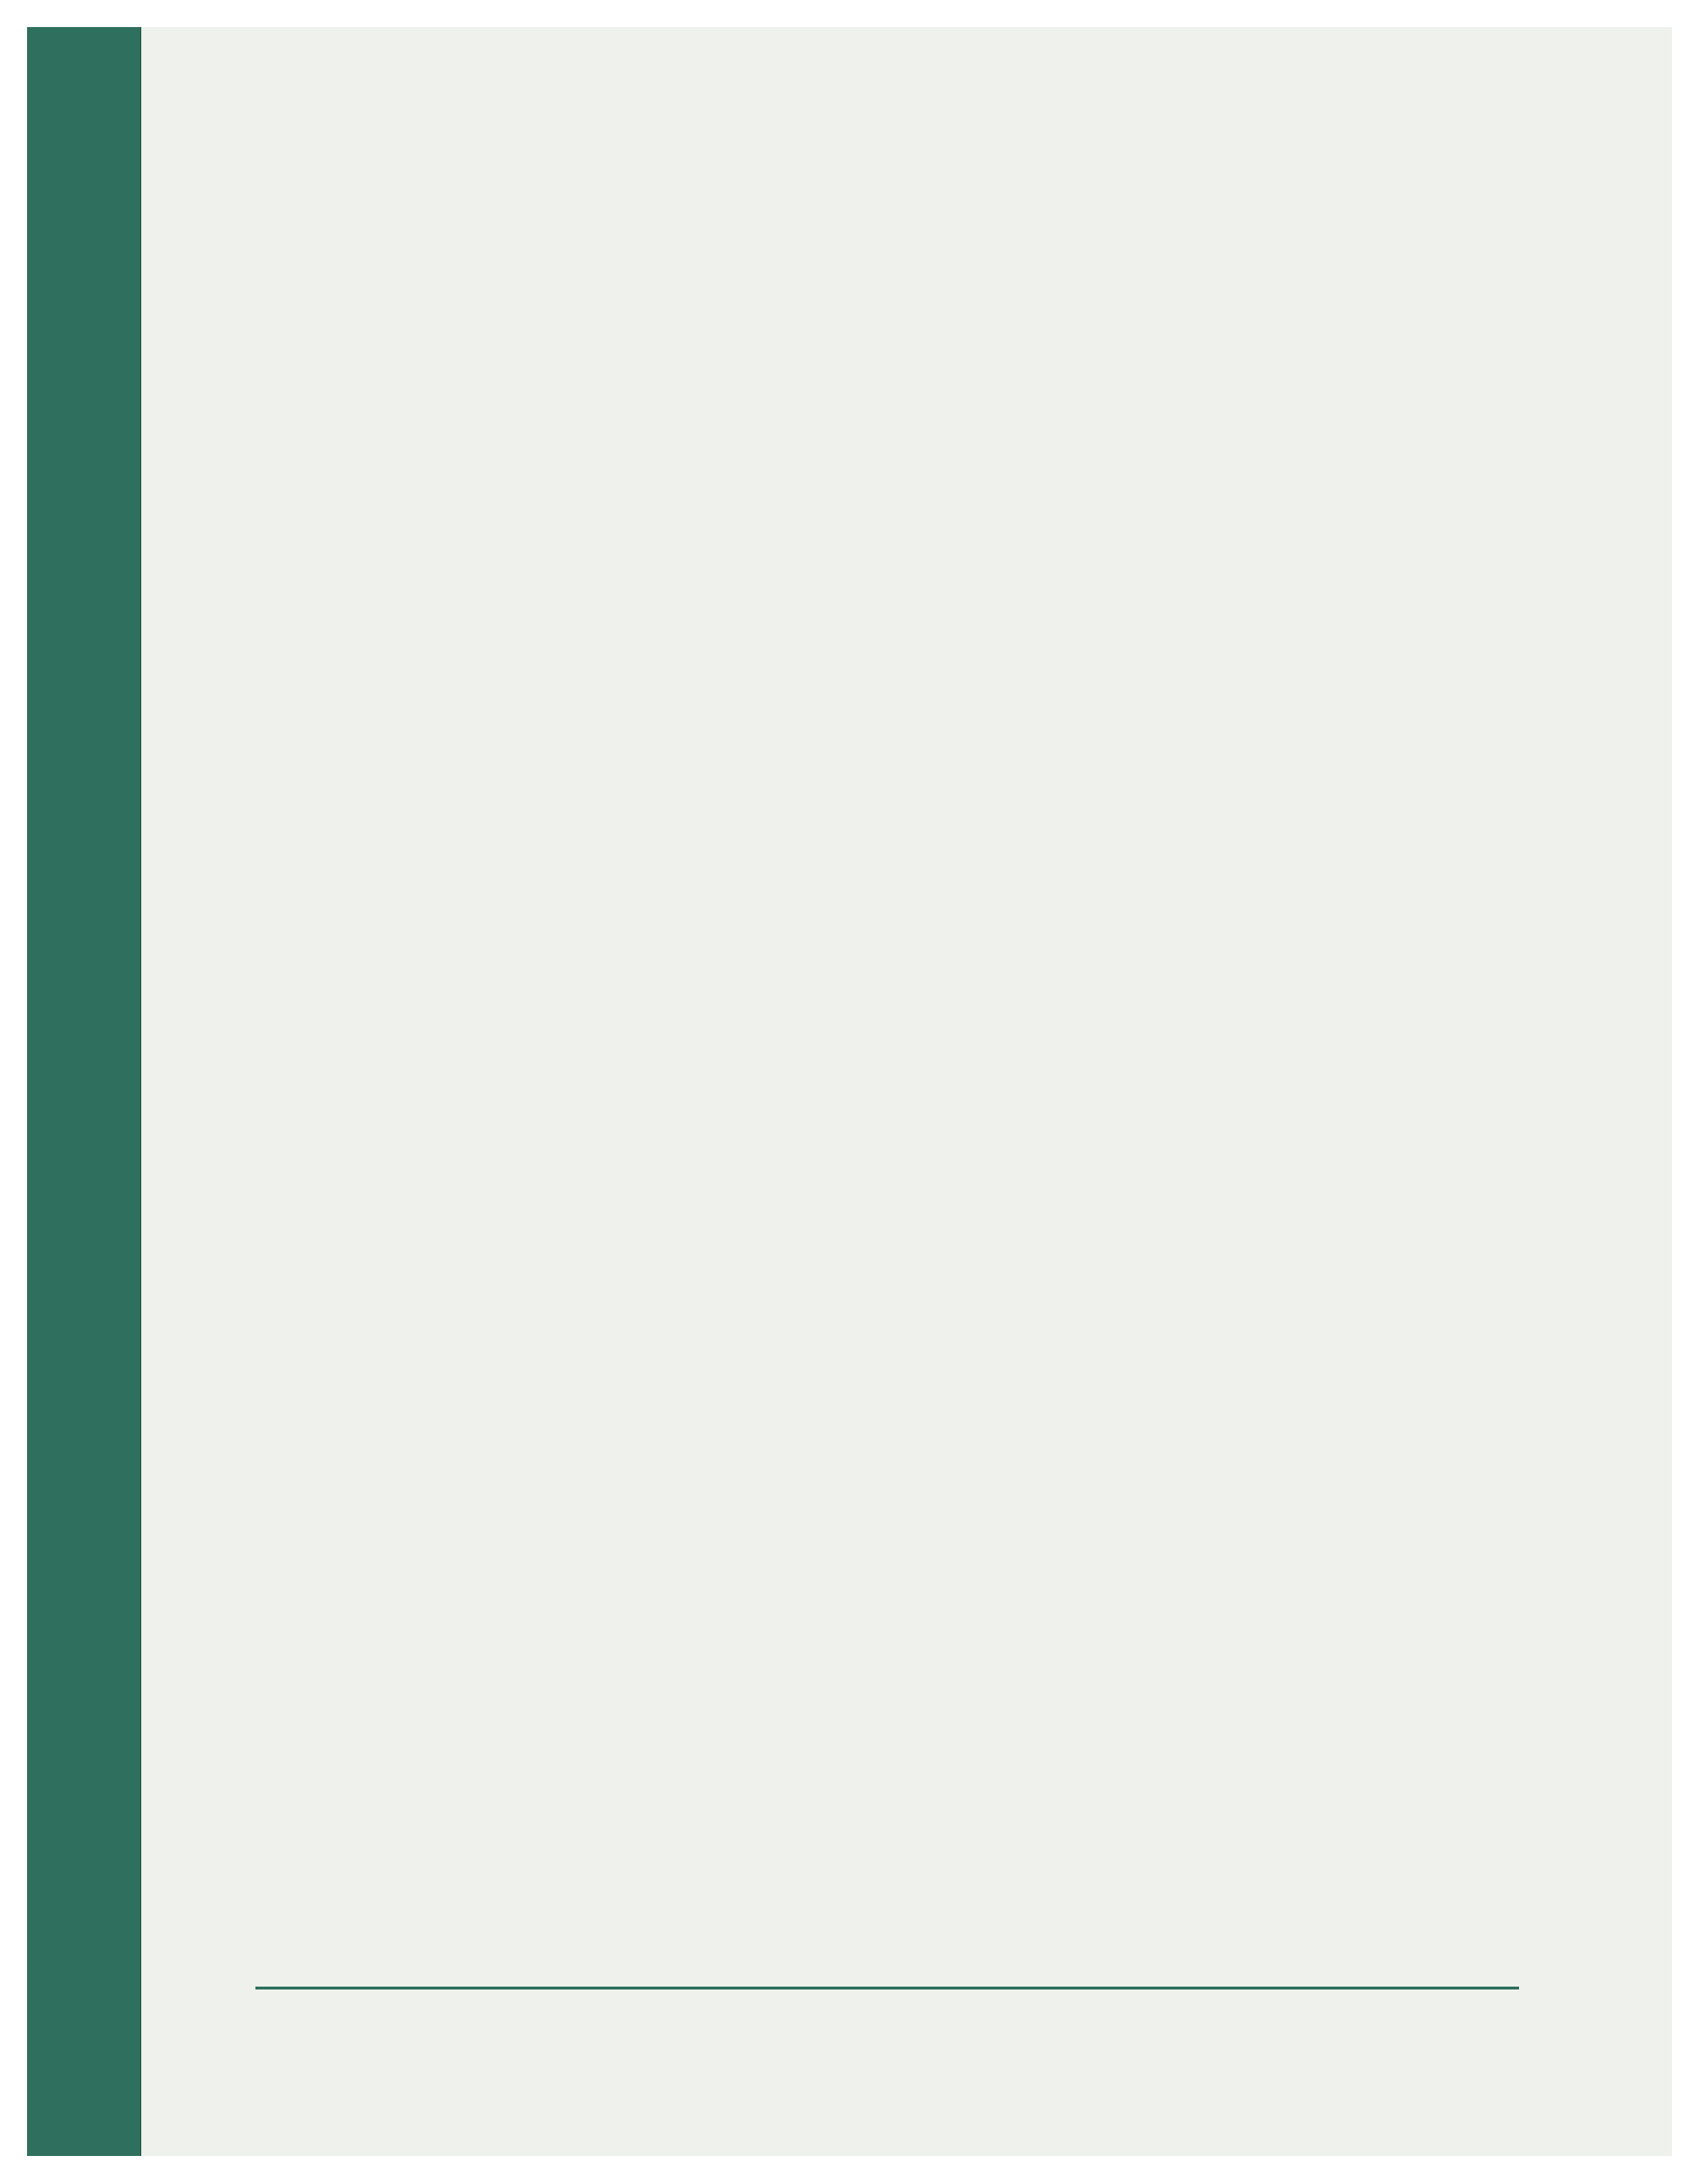
\begin{tikzpicture}
    \fill[paper](0,0) rectangle (\paperwidth,\paperheight);
    \fill[celadon](0,0) rectangle (15mm,\paperheight);
    \draw[celadondk,line width=.3pt](15mm,0)--(15mm,\paperheight);
    \draw[celadon,line width=1pt](30mm,22mm)--(\dimexpr\paperwidth-20mm\relax,22mm);
  \end{tikzpicture}}}}

\begin{document}
\frontmatter
\pagestyle{empty}

% ===================== 표지 =====================
\coverbg
\thispagestyle{empty}
\null\vspace*{34mm}
\begin{center}
  {\sffamily\normalsize\color{celadondk}\addfontfeature{LetterSpace=8} 장-뇌축 설계 모노그래프}\\[3mm]
  {\sffamily\small\color{muted}\addfontfeature{LetterSpace=18} GUT–BRAIN AXIS MONOGRAPH}\\[24mm]
  {\sffamily\bfseries\color{ink}\fontsize{86}{92}\selectfont 힘뇌장}\\[8mm]
  {\sffamily\LARGE\color{celadondk}\addfontfeature{LetterSpace=26} HIMNOEJANG}\\[18mm]
  \begin{tikzpicture}\node[fill=seal,rounded corners=2pt,inner sep=0pt,minimum size=16mm,text=white]{\sffamily\bfseries\LARGE 序};\end{tikzpicture}\\[14mm]
  {\large\color{ink} 전통과 현대를 잇는 장-뇌 설계 — 열두 원료, 하나의 계(系)}
\end{center}
\vfill
\begin{center}
  \textcolor{celadon}{\rule{46mm}{1pt}}\\[5mm]
  {\sffamily\normalsize 기획·감수 \textbf{최성화} \quad 서울대학교 생명과학부}\\[2.5mm]
  {\sffamily\small\color{muted} 작성 Claude (Anthropic) · 4개 전용 스킬}\\[8mm]
  {\sffamily\footnotesize\color{celadondk}\addfontfeature{LetterSpace=4} 보(補) · 연결(連結) · 평정(平靜) · 기능성 보조}
\end{center}
\vspace*{6mm}
\clearpage
\pagestyle{plain}


%% ===== 서문 =====

\chapter*{서문 — 힘뇌장이란 무엇인가}\addcontentsline{toc}{chapter}{서문 — 힘뇌장이란 무엇인가}\markboth{서문 — 힘뇌장이란 무엇인가}{}

\begin{authnote}\textbf{원고 성격.} 이 서문은 본론(제1\textasciitilde{}15장)에 앞서 \textbf{힘뇌장이 무엇이며, 왜·누구를 위해 만들어졌는지}를 먼저 밝히는 글이다. 개별 원료의 학술 인용은 두지 않으며(전권의 근거와 4단계 검증 방법론은 제1장에서 상술한다), 이 책이 쓰인 방식 — 기획·감수와 AI 작성의 역할 분담 — 도 투명하게 적는다.\end{authnote}
\section{왜 이 책을 쓰는가}
발표를 앞둔 강의실 복도에서, 시험지를 받아 든 고사장에서, 마감이 코앞인 사무실에서 — 우리는 종종 "머리가 안 돌아간다"고 말한다. 정작 집중이 가장 필요한 순간에 손끝이 차가워지고 생각이 하얘지는 이 경험은, 뇌만의 문제가 아니다. 스트레스는 장(腸)을 조이고, 장은 다시 뇌에 신호를 보낸다. 지난 십수 년의 신경과학이 밝혀낸 이 양방향의 대화, 곧 \textbf{장-뇌축(gut–brain axis)} 이 이 책의 출발점이다.

나는 오랫동안 이 장-뇌의 대화를 연구하고 가르쳐 오면서 한 가지 물음을 품게 되었다. 조선의 선조들이 스트레스로 속이 무너질 때 비위(脾胃)를 다스려 마음을 다스렸던 그 오랜 지혜를, 현대 과학의 규율로 다시 검증하고 계승할 수는 없을까. 힘뇌장은 그 물음에 대한 하나의 대답이다.

\section{힘뇌장이란 무엇인가}
힘뇌장(HIMNOEJANG)은 \textbf{장에서부터 뇌를 돌보는 것} 을 설계 원리로 삼은 \textbf{일반식품 포뮬러} 다. 열두 가지 원료를 세 개의 축 위에 배치했다 — 소화·흡수의 토대를 세우는 \textbf{보(補)의 축}(사군자탕: 인삼·백출·복령·감초), 장과 뇌를 잇고 신경을 보호하는 \textbf{연결(連結)의 축}(노루궁뎅이버섯·원지), 각성과 이완의 균형을 회복하는 \textbf{평정(平靜)의 축}(L-테아닌·L-티로신·L-글루타민). 여기에 항염·프리바이오틱·완서방출 에너지를 맡는 기능성 보조 원료(커큐민·FOS·팔라티노스)가 더해져, 포뮬러 전체의 장-뇌 환경을 조성한다.

이름 그대로다 — \textbf{'힘'을 주어 '뇌'와 '장'을 함께 돌본다.} 힘뇌장은 의약품이 아니며, 어떤 질병을 치료하거나 예방한다고 말하지 않는다. 다만 하나의 강한 표적을 때리기보다, 장-뇌라는 하나의 계(系)를 여러 지점에서 부드럽게 조율하려는 식품이다.

\section{설계 철학}
힘뇌장의 설계에는 세 가지 태도가 흐른다.

\textbf{첫째, 계(系)의 관점.} 뇌 건강을 고립된 장기의 문제가 아니라 장·면역·대사·정신을 아우르는 네트워크의 문제로 본다. 그래서 하나의 성분이 아니라 여러 원료의 조율, 곧 포뮬러를 택했다.

\textbf{둘째, 전통과 현대의 연속성.} 사군자탕·개심산 같은 전통 복합처방의 지혜를 버리지도, 맹신하지도 않는다. 원료마다 현대 문헌으로 검증하여, 전통이 과학과 공명하는 지점을 잇는다.

\textbf{셋째, 겸손과 정직.} 근거가 확실한 것과 아직 유망한 수준인 것을 등급으로 구분하고, 효과가 없었던 연구(무효 결과)와 한계까지 그대로 적는다. 근거의 언어는 "관련성이 보고되었다"이지 "낫는다"가 아니다.

\section{누구를 위한 것인가}
이 책과 힘뇌장은 특히 \textbf{시험과 마감, 발표와 경쟁 앞에서 최상의 집중을 요구받는 사람들} 을 마음에 두고 만들어졌다 — 수험생과 학생, 고강도 인지 노동을 하는 직장인, 스트레스 속에서도 평정을 잃지 않아야 하는 이들. 나아가 나이 듦 속에서 또렷함을 지키고 싶은 분들, 장과 마음의 균형이 흔들려 회복이 필요한 분들에게도.

이들이 힘뇌장이라는 식품으로 조금이나마 \textbf{도움을 받았으면 하는 바람} 으로 이 자료를 설계했다. 다만 분명히 해 둔다. 힘뇌장은 일반식품이며, 여기 담긴 근거의 상당 부분은 인체 대규모 확증 이전의 연관성(association) 수준이다. 이 책은 무엇도 보장하지 않는다 — 다만 각 원료가 어떤 근거 위에 서 있는지를 투명하게 보여줄 뿐이다. 건강에 관한 결정은 늘 전문가와 상의하시기를 권한다.

\section{이 책은 어떻게 쓰였는가 — 기획·감수와 AI 작성}
이 방대한 자료의 저자됨을 정직하게 밝히는 것이 이 서문의 중요한 목적이다. 이 책은 \textbf{최성화 교수가 기획·설계·감수} 하고, \textbf{Claude(Anthropic의 대규모 언어모델)를 기반으로 구축한 네 개의 전용 스킬이 작성} 하였다. 표현하자면, \textbf{기획·감수 최성화 / 작성 Claude} 다.

작성은 다음 네 스킬의 협업으로 이루어졌다.

\begin{enumerate}[leftmargin=6mm,itemsep=1pt,topsep=2pt]
  \item \textbf{chapter-drafter} — 15섹션 표준 템플릿에 따라 각 장의 초고를 작성.
  \item \textbf{reference-validator} — 모든 학술 인용을 CrossRef·PubMed로 4단계 검증(DOI 존재 → 제목 완전 일치 → 저자·연도 교차 → PMID 대조). 통과한 인용에만 검증 태그를 부여하고, 존재하지 않는 논문을 지어내는 '환각(hallucination)'을 원천 차단했다.
  \item \textbf{historical-verifier} — 조선 사료 인용의 원전 정확성을 국가 DB와 대조하는 절차(소설·드라마는 배제). 다만 확정 인용은 최소화하고 논쟁의 여지 없는 배경 사실만 서술했다.
  \item \textbf{chapter-editor} — 식품 표시광고 규제 준수·학술 용어 통일·저자 톤 유지·근거 수준 표현을 최종 점검.
\end{enumerate}
그 결과 이 책의 \textbf{826편에 이르는 인용은 예외 없이 실측·검증} 을 거쳤다. 존재하지 않는 논문, 지어낸 저자, 맞지 않는 DOI는 이 책에 없다. 이것이 독자가 이 책을 신뢰해도 좋은 근거다.

동시에 \textbf{한계} 도 분명히 밝힌다. 본문은 AI가 작성한 초고이며, 저자(최성화 교수)의 최종 감수·승인이 전제되어야 완성된다. AI는 검증의 규율에도 불구하고 해석의 오류를 범할 수 있으므로, 이 책은 '확정된 결론'이 아니라 \textbf{'검증된 근거 위에 선 설계 논증'} 으로 읽혀야 한다. 또한 개별 원료 각각의 근거가 곧 포뮬러 전체의 근거는 아니며, 힘뇌장 자체에 대한 대규모 인체 시험은 앞으로의 과제다. \textbf{신뢰와 한계 — 이 둘을 함께 느끼며 읽어 주시기를} 부탁드린다.

\section{맺음}
이 책은 하나의 제품 설명서가 아니라, 뇌 건강을 계로 바라보고 전통을 과학으로 잇는 하나의 태도에 관한 기록이다. 첫걸음은 사백 년 전, 전란의 한복판에서 심신을 다스려야 했던 한 장수의 이야기에서 시작한다. 이제, 그 여정을 함께 시작한다.

\textbf{기획·감수} 최성화 (서울대학교 생명과학부)

\textbf{작성} Claude (Anthropic) · chapter-drafter · reference-validator · historical-verifier · chapter-editor

2026년


\clearpage
\tableofcontents
\clearpage

\mainmatter
\pagestyle{fancy}


%%%%% CH 1 %%%%%

\chapter{총론 — 왜 이 책인가}

\section{프롤로그 — 어느 봄날의 실험실}
매년 봄이 오면 나는 같은 얼굴들을 본다. 서울대학교 생명과학부의 대학원생들, 그리고 진로를 고민하는 학부생들. 그들은 대개 유능하고, 성실하며, 무엇보다 지쳐 있다. 논문 마감과 실험 실패, 진로에 대한 불안이 겹치는 계절이면, 젊은 뇌들은 카페인과 밤샘으로 스스로를 몰아붙인다. 나는 30년 가까이 이 풍경을 지켜보았고, 한 가지 질문을 놓지 못했다. \textbf{왜 우리는 이토록 열심히 살면서도, 정작 뇌를 돌보는 법은 배우지 못했는가?}

이 질문은 사적인 것이 아니다. 그것은 오늘날 한국 사회 전체의 질문이다. 우리는 세계에서 가장 빠르게 성장한 나라를 만들었지만, 그 대가로 만성적인 긴장과 피로, 불면과 소진(burnout)을 일상의 배경음으로 삼게 되었다. 뇌는 쉬는 법을 잊었고, 몸은 늘 경계 상태다. 병원에 갈 만큼 아프지는 않지만, 온전히 건강하지도 않은 — 이 광범위한 회색지대에 수많은 현대인이 머물러 있다.

이 책은 그 회색지대를 향한 하나의 응답이다. 그러나 나는 만병통치의 비약(祕藥)을 말하려는 것이 아니다. 오히려 정반대다. 이 책은 \textbf{엄격하게 검증된 과학적 근거의 언어로, 한국인의 오랜 심신(心身) 돌봄의 지혜를 재해석하려는 시도}다. 그 중심에는 힘뇌장(HIMNOEJANG)이라는 하나의 기능성 포뮬러가 있지만, 이 책의 진짜 주제는 제품이 아니라 \textbf{철학} — 즉, 장(腸)과 뇌(腦)를 하나의 계(系)로 바라보는 관점, 그리고 전통과 현대 과학을 잇는 설계의 원리다.

이 첫 장에서 나는 네 가지를 이야기하려 한다. 첫째, 우리가 마주한 문제(현대인의 뇌 피로와 만성 스트레스)의 실체. 둘째, 그 문제를 새롭게 이해하게 해준 과학적 패러다임의 전환(장-뇌축). 셋째, 왜 나는 다시 '보약(補藥)'의 전통으로 눈을 돌렸는가. 넷째, 이 책이 스스로에게 부과한 근거의 규율 — 무엇을 주장하고, 무엇을 주장하지 않을 것인가. 그리고 마지막으로, 앞으로 열네 개의 장이 어떻게 전개될지를 안내한다.

시작은, 언제나 그렇듯, 지쳐 있던 한 젊은 얼굴이다.

\section{문제 제기 — 현대인의 뇌는 왜 지치는가}
\subsection{소진(Burnout)이라는 시대의 증후군}
번아웃은 더 이상 소수의 문제가 아니다. 세계보건기구가 이를 직업 관련 현상으로 분류한 이래, 소진은 현대 노동사회의 광범위한 증후군으로 자리 잡았다. 의료·간호처럼 고부담 직군을 대상으로 한 대규모 체계적 문헌고찰들은 소진의 유병률이 직군과 측정도구에 따라 크게 달라지되, 결코 무시할 수 없는 수준임을 반복적으로 보여준다. 의사를 대상으로 한 대규모 체계적 문헌고찰[1], 정신건강 간호사[2]·중환자실 간호사[3]·완화의료 간호사[7]·소화기내과 의사[6]·치과의사[4], 그리고 중국 의사 집단[5]에 대한 메타분석은 공통적으로 높은 소진 부담과 그 위험요인(과중한 업무·자율성 결여·정서적 소모)을 지목한다.

이 통계들이 말하는 바는 분명하다. 소진은 개인의 나약함이 아니라 \textbf{구조적·생물학적 현상}이라는 것이다. 그리고 그 생물학의 중심에 만성 스트레스가 있다.

\subsection{만성 스트레스와 뇌 — 전전두엽에서 해마까지}
급성 스트레스는 적응적이다. 위협 앞에서 우리를 각성시키고 집중하게 한다. 문제는 그것이 \textbf{만성화}될 때다. 만성 스트레스는 뇌의 고차 인지를 담당하는 전전두엽(prefrontal cortex) 네트워크를 약화시킨다. Arnsten의 고전적 정리[8]에 따르면, 지속적 스트레스는 전전두엽의 시냅스 연결을 분자 수준에서 손상시켜 주의·작업기억·자기조절 능력을 저하시키고, 대신 편도체 중심의 습관적·반사적 회로에 통제권을 넘긴다. 우리가 지쳤을 때 사소한 일에 예민해지고, 계획적 사고 대신 충동에 휘둘리는 이유가 여기에 있다.

만성 스트레스의 표적은 전전두엽에 그치지 않는다. 시상하부-뇌하수체-부신(HPA) 축의 만성적 활성화는 코르티솔의 지속적 상승을 낳고, 이는 해마(hippocampus)의 신경가소성과 신경발생을 저해하며 신경염증을 촉진한다[9]. 청소년기의 스트레스는 흥분-억제(E/I) 균형과 인지 임계기 가소성을 교란하며[11], 심리적 스트레스와 우울의 접점에는 중추-말초를 잇는 신경면역(neuroimmune) 동역학이 자리한다[10].

\subsection{알로스타틱 부하와 코르티솔 — 축적되는 마모}
이러한 만성적 마모를 개념화한 것이 \textbf{알로스타틱 부하(allostatic load)} — 스트레스에 대한 반복적 적응이 누적되며 신체·뇌에 남기는 '마모의 총합'이다. 알로스타틱 부하와 뇌 구조·기능의 연관을 정리한 체계적 문헌고찰[13]은, 만성 스트레스가 측정 가능한 뇌 변화로 이어짐을 보여준다. McEwen은 이 부하가 고정된 손상이 아니라 회복탄력성(resilience)·후성유전·뇌 가소성을 통해 조절 가능한 과정임을 강조했다[12] — 이는 개입의 여지가 있다는 희망의 근거이기도 하다.

코르티솔은 이 과정의 핵심 지표다. 일주기 코르티솔 기울기의 이상은 다양한 정신·신체 건강 결과와 연관되며[14], 코르티솔 조절 이상은 청소년·청년기 우울의 발생과도 관련된다[15]. 만성 불면 환자에서 관찰되는 HPA 축 과활성[16]은 스트레스-수면-각성의 악순환을 보여준다. 다행히 스트레스 관리 개입이 코르티솔 수준을 실제로 변화시킬 수 있다는 메타분석 근거[17]는, 이 축이 조절 가능한 표적임을 시사한다.

\subsection{문제의 요약 — 회색지대의 생물학}
요약하면, 현대인의 '뇌 피로'는 막연한 은유가 아니라 구체적 생물학이다. 만성 스트레스 → HPA 축 과활성 → 코르티솔 이상 → 전전두엽·해마 손상과 신경염증 → 인지·정서 기능 저하로 이어지는 이 연쇄는, 질병으로 진단되기 이전의 광범위한 기능 저하 상태 — 내가 앞서 '회색지대'라 부른 영역 — 를 만든다. 바로 이 회색지대야말로 힘뇌장이 겨냥하는 지점이다. 그리고 이 영역을 새롭게 이해하는 열쇠가, 지난 20년간 신경과학을 뒤흔든 하나의 패러다임 전환에서 나왔다.

\section{패러다임 전환 — 장-뇌축의 부상}
\subsection{"머리로만 생각한다"는 오해}
오랫동안 우리는 뇌를 고립된 사령탑으로 여겼다. 정신은 두개골 안에서 완결되며, 소화관은 그저 영양을 흡수하는 관(管)일 뿐이라고. 그러나 지난 20년의 연구는 이 그림을 근본적으로 바꾸었다. 오늘날 우리는 안다 — 장과 뇌는 신경·면역·내분비·대사의 여러 경로로 끊임없이 대화하는 \textbf{하나의 통합된 계}이며, 그 대화의 상당 부분을 장내미생물총(gut microbiota)이 매개한다는 것을.

이 \textbf{장-뇌축(gut-brain axis, 腸-腦軸)}, 더 정확히는 \textbf{미생물총-장-뇌축(microbiota-gut-brain axis)} 개념은 이제 소화기·신경·정신의학을 가로지르는 통합 프레임워크가 되었다[19][21]. 장은 "제2의 뇌"라 불릴 만큼 방대한 장신경계(enteric nervous system)를 갖고, 신경전달물질과 그 전구체를 생산하며, 면역계의 최대 접점이자 미생물 대사의 무대다. 장의 상태는 곧 뇌의 상태에 영향을 미친다.

\subsection{네 갈래의 대화 경로}
장-뇌축의 소통은 크게 네 경로로 정리된다. 이 틀은 이후 여러 종합 리뷰에서 반복적으로 확인·정교화되었다[22][23][24].

\begin{enumerate}[leftmargin=6mm,itemsep=1pt,topsep=2pt]
  \item \textbf{신경 경로 — 미주신경(vagus nerve).} 장과 뇌를 직접 잇는 미주신경은 장내 신호를 중추로 전달하는 고속도로다. 미주신경은 미생물총-장-뇌 소통의 핵심 인터페이스이며[27], 인지 통제[28]와 신경정신 기능[29]에 관여한다.
  \item \textbf{면역 경로.} 장은 인체 면역의 최대 기관이다. 만성 스트레스는 장-면역 상호작용을 교란하고, 이 신호는 신경염증을 통해 뇌로 전달된다[35].
  \item \textbf{내분비·HPA 경로.} 장내미생물총은 HPA 축과 양방향으로 작용하며 스트레스 반응성을 조절한다[22][34].
  \item \textbf{대사산물 경로.} 미생물이 만드는 대사산물, 특히 \textbf{단쇄지방산(short-chain fatty acids, SCFA)} 은 장벽·면역·신경을 매개로 뇌 기능에 영향을 미친다. SCFA의 미생물총-장-뇌 소통에서의 역할은 대규모 리뷰로 정리되었고[25], 신경퇴행 맥락에서도 검토되었다[26].
\end{enumerate}
\subsection{식이·미생물·뇌 — 개입 가능한 축}
이 패러다임이 특별히 중요한 이유는, 장-뇌축이 \textbf{개입 가능한(modifiable)} 축이라는 데 있다. 유전자와 달리 우리는 먹는 것을 바꿀 수 있고, 식이는 장내미생물총을 통해 뇌에 도달한다. "식이-미생물총-장-뇌축"을 정리한 리뷰[30]와, 좋은 정신건강의 씨앗으로서 식이의 역할을 조망한 대규모 리뷰[31]는, 영양이 곧 뇌 건강의 지렛대가 될 수 있음을 보여준다. 장과 뇌 사이의 장벽(gut·brain barriers)이 소통의 관문으로 작동한다는 최신 정리[20]는 이 축의 구조적 기반을 제시한다.

임상 근거도 축적되고 있다. 주요우울장애 환자에서 장내미생물총의 조성 변화가 메타분석으로 보고되었고[32][33], 미생물총-장-뇌축은 다양한 신경정신 질환의 병태생리와 연결된다[36][37]. 물론 이 근거들은 대부분 연관성(association) 수준이며, 인과의 방향과 크기는 여전히 활발히 연구 중이다. 그러나 방향성은 분명하다 — \textbf{뇌를 돌보려면 장을 함께 보아야 한다.}

\subsection{이 책의 이론적 토대}
장-뇌축은 힘뇌장 설계 철학의 이론적 토대 그 자체다. 이 패러다임의 형성 과정 — 무균(germ-free) 마우스 실험에서 시작해 Cryan 등(2019)의 종합적 리뷰[18]에 이르는 과학사 — 는 제3장에서 상세히 다룬다. 여기서 기억할 것은 하나다: 힘뇌장의 여덟 원료는 '뇌에 좋은 것'을 무작위로 모은 것이 아니라, \textbf{장-뇌축이라는 하나의 계를 여러 노드에서 조율한다는 설계 원리} 위에 배치되었다는 점이다.

\section{왜 다시 '보약'인가 — 전통과 현대의 만남}
\subsection{폄하되었던 지혜}
장-뇌축의 언어로 무장한 현대 과학이 뒤늦게 도달한 결론 — "장을 다스려 마음을 다스린다" — 는, 사실 동아시아 전통의학이 수백 년간 견지해 온 관점이다. 한의학은 비위(脾胃)를 후천지본(後天之本)으로 삼아 소화·흡수의 토대가 곧 정신의 토대라 보았고, "심주신명(心主神明)"과 "비주사(脾主思)"의 언어로 소화와 사고를 연결했다. 나는 이것을 신비주의로 낭만화할 생각이 없다. 그러나 그것을 미신으로 폄하하는 것 역시 과학적 태도가 아니다.

전통 본초에 대한 현대적 재조명은 이미 상당한 근거를 축적했다. 정신질환에 대한 약초 치료를 10년 단위로 정리한 리뷰[38], 불안·우울·불면에 대한 약초 근거[39][40], 우울의 신경가소성 가설에서 전통 한약재의 역할[42], 알츠하이머병에 대한 전통 한의학의 체계적 문헌고찰[43], 인지장애에 대한 파이토테라피의 신경혈관·교세포(neurovascular glial unit) 표적[41], 뇌졸중 재활에서 서양의학과 전통의학의 통합적 접근[44] 등은, 전통 본초가 현대 임상연구의 대상으로 진지하게 다뤄지고 있음을 보여준다.

\subsection{적응원(Adaptogen)과 자연의 항스트레스 물질}
특히 주목할 것은 '적응원(adaptogen)' 개념이다. 스트레스에 대한 신체의 저항력을 비특이적으로 높인다고 알려진 이 식물군은, 역사적 전통과 현대적 전망을 함께 갖는다[45]. 개별 성분 수준에서도 근거가 쌓이고 있다 — 아쉬와간다의 불안·불면에 대한 체계적 문헌고찰·메타분석[46], 사프란의 신경·정신 질환 근거[47], 레몬밤(멜리사)의 우울·불안 임상 근거[48], 라벤더의 불안 메타분석[49], 백작약 유래 알비플로린(albiflorin)의 신경·정신 질환 근거[53] 등이 그 예다. 식물 유래 향인지(nootropic) 성분과 인간 인지의 관계[50], 정신건강·뇌 기능에 대한 식물 유래 뉴트라수티컬의 기전과 잠재력[51]을 정리한 리뷰들은, 전통 지식이 현대 성분과학으로 번역될 수 있음을 보여준다.

물론 이 근거들에는 일관되게 따라붙는 단서가 있다 — 표본이 작고, 제형과 용량이 이질적이며, 방법론적 질이 고르지 않다는 것. 불안·강박에 대한 중국 약초의 체계적 문헌고찰[52]을 비롯한 다수 연구가 "유망하나 확정적이지 않다"는 신중한 결론으로 수렴한다. 이 신중함은 약점이 아니라, 본 책이 견지하는 태도의 출발점이다(§7).

\subsection{'K-보약'의 재구성}
한국에는 고유의 보약(補藥) 전통이 있다. 그것은 단순히 '몸에 좋은 것을 먹는' 습관이 아니라, 심신을 하나로 보고 근본(本)을 북돋아 균형을 회복시킨다는 정교한 설계 사상이었다. 사군자탕(四君子湯)이 기(氣)를 세우고 비위를 보하는 골격이라면, 여기에 안신(安神)·개규(開竅)의 원료를 더해 정신을 다스리는 것이 전통 처방의 논리다.

내가 이 책에서 시도하는 것은 이 전통을 \textbf{현대 장-뇌축 과학의 언어로 재구성}하는 일이다. 그것은 복고(復古)가 아니라 번역(飜譯)이다. 조상들이 경험적으로 알았던 것을, 우리는 이제 수용체와 미생물과 대사산물의 언어로 다시 쓸 수 있다. 힘뇌장은 그 번역의 구체적 결과물이며, K-웰니스(K-Wellness)라는 더 큰 문화적 서사의 한 실천이다.

\section{힘뇌장이라는 답 — 설계 철학의 개요}
\subsection{세 개의 축}
힘뇌장은 여덟 개의 원료로 구성되지만, 그 설계는 세 개의 축(軸)으로 이해할 때 가장 명료하다.

\vspace{2pt}\noindent{\footnotesize\begin{tabularx}{\linewidth}{@{}*{4}{>{\raggedright\arraybackslash}X}@{}}
\toprule
\textbf{축} & \textbf{역할} & \textbf{해당 원료} & \textbf{장-뇌축 접점} \\
\midrule
\textbf{보(補)의 축} & 기(氣)를 세우고 소화·흡수의 토대를 다짐 & 인삼·백출·복령·감초 (사군자탕) & 비위·장벽·흡수 \\
\textbf{연결(連結)의 축} & 장과 뇌를 잇고 신경영양을 지원 & 노루궁뎅이버섯·법제 원지 & 신경영양(NGF)·신경보호 \\
\textbf{평정(平靜)의 축} & 각성-이완의 균형을 회복 & L-테아닌 (+ L-티로신·L-글루타민 등 보조) & GABA/글루탐산·α파·HPA \\
\bottomrule
\end{tabularx}}\vspace{3pt}

이 세 축은 서로 겹치지 않으면서 하나의 계를 완성한다. 보의 축이 토대를, 연결의 축이 다리를, 평정의 축이 균형을 담당한다. 여기에 커큐민(항염)·FOS(프리바이오틱스)·팔라티노스(완서방출 에너지) 등 기능성 보조 원료가 더해져 포뮬러 전체의 장-뇌 환경을 조성한다.

\subsection{왜 '단일 성분'이 아니라 '포뮬러'인가}
현대 영양과학의 한 흐름은 단일 성분의 극적 효과를 좇는다. 그러나 나는 이 접근이 뇌-장이라는 복잡계에는 부적합하다고 본다. 장-뇌축은 다중 경로·다중 노드의 네트워크이며, 이런 계는 하나의 강한 개입보다 \textbf{여러 지점의 부드러운 조율}에 더 잘 반응할 가능성이 높다. 정신질환에 대한 뉴트라수티컬·파이토수티컬 임상 지침을 제시한 WFSBP·CANMAT 전문가 태스크포스의 종합[55]은, 복합적·다표적 접근이 정신건강 영역에서 진지하게 고려되고 있음을 보여준다. 발효식품이 미생물총-장-뇌축을 통해 정신건강을 조절할 잠재력을 정리한 리뷰[56], 지역사회 고령자에서 프로바이오틱스 보충이 인지·기분과 장내미생물총 변화와 관련됨을 보고한 국내 다기관 RCT[57]는, 복합적 식이 개입이 인체에서 측정 가능한 변화와 관련됨을 시사한다.

힘뇌장의 설계 사상은 이 관점 위에 있다 — \textbf{하나의 표적을 강하게 때리기보다, 하나의 계를 여러 노드에서 조율한다.} 각 원료의 구체적 근거와 배합 정당성은 제4장 이후에서 원료별로 상세히 논증한다.

\section{이 책의 방법론 — 검증의 규율}
\subsection{왜 방법론을 앞세우는가}
건강·영양 분야만큼 잘못된 정보가 범람하는 영역도 드물다. 블로그와 상품 페이지, 검증되지 않은 '카더라'가 근거의 외양을 두르고 유통된다. 더욱이 생성형 AI의 시대에는 존재하지 않는 논문을 그럴듯하게 지어내는 이른바 '환각(hallucination)'의 위험까지 더해졌다. 그래서 나는 이 책의 내용을 말하기 전에, 이 책이 \textbf{어떻게 쓰였는지}를 먼저 밝히고자 한다. 방법론의 투명성은 신뢰의 전제다.

\subsection{참고문헌 4단계 검증 — Anti-Hallucination}
본 책의 모든 학술 인용은 예외 없이 다음 4단계 검증을 통과한다.

\begin{enumerate}[leftmargin=6mm,itemsep=1pt,topsep=2pt]
  \item \textbf{DOI 존재 확인} — 모든 인용의 DOI를 CrossRef에서 실제 조회한다.
  \item \textbf{제목 완전 일치} — DOI가 가리키는 실제 논문 제목과 인용 제목의 일치를 확인한다(환각 차단의 핵심 신호).
  \item \textbf{저자·저널·연도 교차 확인} — 메타데이터의 정합성을 검증한다.
  \item \textbf{PubMed PMID 교차 확인} — 의학·생물학 문헌은 PubMed에서 PMID로 재확인한다.
\end{enumerate}
이 4단계를 통과한 인용에만 \texttt{[DOI-VERIFIED ✓]} 태그를 부여하며, 실패한 인용은 삭제하거나 대체한다. 인용 가능한 소스는 Tier 1–3 학술지(Nature·Science·Cell·Lancet·NEJM 계열 및 확립된 peer-review 저널)로 한정하고, 개인 블로그·상품 페이지·대중매체·검증 없는 AI 응답 등은 원천 배제한다. 실제로 본 방법론을 적용한 제10장(L-테아닌)에서는 82편의 인용 전체가 검증을 통과했다.

\subsection{조선 사료의 원전 검증}
역사 서술 — 특히 제2장의 조선시대·이순신 관련 내용 — 에는 별도의 사료 검증 프로토콜을 적용한다. 난중일기·조선왕조실록·동의보감 등의 인용은 국사편찬위원회·규장각·한국한의학연구원 등 국가 DB의 원본과 대조하며, 소설·드라마 등 허구적 각색은 인용에서 절대 배제한다. 확인 불가능한 사료는 확정 인용하지 않고 명시적으로 표시한다.

\subsection{근거 수준의 등급화(GRADE)}
각 원료의 근거는 GRADE 방법론에 따라 영역별로 등급화한다. 등급은 '효능의 크기'가 아니라 '근거의 신뢰도'를 나타내며, 이를 통해 독자는 어떤 주장이 얼마나 확실한 근거 위에 서 있는지를 투명하게 판단할 수 있다. 유망한 근거와 확립된 근거를 구별하는 이 규율이야말로, 이 책이 상업적 과장과 구별되는 지점이다.

\section{근거의 태도 — 무엇을 주장하고, 무엇을 주장하지 않는가}
\subsection{겸손이라는 과학적 미덕}
나는 이 책에서 힘뇌장이 무엇을 '치료'하거나 '예방'한다고 말하지 않을 것이다. 그것은 규제(식품의약품안전처 표시광고 규정)의 문제일 뿐 아니라, 무엇보다 \textbf{과학적 정직성}의 문제다. 힘뇌장은 일반식품이며, 의약품이 아니다. 이 책이 다루는 근거의 상당 부분은 연관성(association)과 가능성의 수준에 있고, 인체 대규모 확증 시험은 아직 충분하지 않다.

실제로, 이 분야의 최신 종합들은 한결같이 신중하다. 정신·인지 장애에 대한 정신생물학(psychobiotics)의 무작위배정 임상시험을 정리한 체계적 문헌고찰[58], 우울에 대한 정신생물학의 체계적 문헌고찰[59], 프로바이오틱스에서 정신생물학으로의 개념적 전환을 조망한 리뷰[60], 노화기 인지에 대한 영양보충제의 임상 근거를 정리한 서술적 리뷰[61], 노년기 인지장애에 대한 영양 개입의 체계적 문헌고찰[54], 프로바이오틱스의 우울에 대한 메타분석[62], 프리·프로바이오틱스의 우울·불안에 대한 대조시험 메타분석[63] 등은 모두 "유익한 신호가 있으나 이질성과 방법론적 한계로 확정적 결론은 이르다"는 취지로 수렴한다. WFSBP·CANMAT 지침[55] 역시 뉴트라수티컬을 표준치료의 대체가 아닌 보조·통합의 맥락에 신중히 위치시킨다.

\subsection{이 책이 주장하는 것}
그렇다면 이 책은 무엇을 주장하는가? 세 가지다.

\begin{enumerate}[leftmargin=6mm,itemsep=1pt,topsep=2pt]
  \item \textbf{설계의 합리성.} 힘뇌장의 여덟 원료가 장-뇌축이라는 일관된 원리 위에 근거를 갖고 배치되었다는 것. 이는 각 원료의 검증된 문헌으로 논증 가능한 주장이다.
  \item \textbf{근거의 투명성.} 각 원료가 어떤 영역에서 얼마나 확실한 근거를 갖는지를, 과장 없이 등급과 함께 제시한다는 것.
  \item \textbf{전통-현대의 연속성.} 한국인의 심신 돌봄 전통이 현대 장-뇌축 과학과 공명하며, 그 번역이 문화적으로도 의미 있다는 것.
\end{enumerate}
\subsection{이 책이 주장하지 않는 것}
반대로 이 책은 다음을 주장하지 않는다 — 힘뇌장이 특정 질병을 치료·예방한다는 것, 개인차를 넘어 모두에게 동일하게 작용한다는 것, 의학적 치료를 대체할 수 있다는 것. 이 경계를 분명히 하는 것이야말로, 독자에 대한 최소한의 예의이자 과학자로서의 책무다. 근거의 언어는 "관련성이 보고되었다", "지원 가능성이 시사된다"이지, "낫는다"가 아니다.

\section{이 책의 구조 — 열다섯 장의 여정}
이 책은 다섯 부(部), 열다섯 장(章)으로 짜여 있다.

\textbf{제1부 · 서장(Prologue)} 은 토대를 놓는다. 제1장(총론)은 지금 이 글이며, 왜 이 책이 필요한지를 논한다. 제2장은 조선시대와 이순신 장군의 사례를 통해 한국형 심신의학의 역사적 뿌리를 추적한다 — 이 장은 사료 원전 검증을 가장 엄격히 적용받는다. 제3장은 무균 마우스 실험에서 Cryan 등(2019)에 이르는 장-뇌축 과학의 재발견사를 정리한다.

\textbf{제2부 · 사군자탕 4원료(Foundation)} 는 보(補)의 축을 다룬다 — 인삼(제4장)·백출(제5장)·복령(제6장)·감초(제7장). 소화·흡수의 토대이자 장-뇌축의 말초 기반을 이루는 원료들이다.

\textbf{제3부 · 장-뇌 특화(Gut \& Brain)} 는 연결과 평정의 축을 다룬다 — 노루궁뎅이버섯(제8장)·법제 원지(제9장), 그리고 L-테아닌(제10장). 신경영양과 각성-이완 균형을 담당하는 핵심 원료들이다.

\textbf{제4부 · 기능성 보조(Cognition \& Resilience)} 는 인지와 회복탄력성을 지원하는 원료를 다룬다 — L-티로신(제11장)·L-글루타민(제12장)·커큐민(제13장)·FOS와 팔라티노스(제14장).

\textbf{제5부 · 종장(Epilogue)} 인 제15장은 여덟 원료의 통합과 시너지, 그리고 미래를 조망한다.

각 원료 장은 동일한 15섹션 표준 템플릿(프롤로그·역사·설계근거·전통의학·현대약리·장-뇌축·동물실험·인체임상·안전성·힘뇌장역할·시너지·한국인의지혜·근거수준·미래·요약)을 따른다. 이 반복 구조는 독자가 원료 간 근거를 공정하게 비교할 수 있게 한다.

마지막으로, 이 책이 궁극적으로 겨냥하는 것은 하나의 제품이 아니라 하나의 태도다 — 뇌 건강을 고립된 장기의 문제가 아니라 장·면역·대사·정신을 아우르는 계(系)의 문제로 보고, 전통의 지혜를 현대 과학의 규율로 검증하며 계승하는 태도. 전 세계적으로 회복탄력성과 뇌 건강을 인구 수준에서 조망하는 최신 연구[64]가 보여주듯, 이는 한국만의 관심사가 아니라 인류 공통의 과제다. 스트레스에 대한 회복탄력성이 운동[65]을 비롯한 여러 개입으로 조절 가능하다는 근거[66]는, 우리가 뇌 건강의 수동적 관찰자가 아니라 능동적 설계자가 될 수 있음을 말해준다.

이제, 그 여정을 시작한다. 첫걸음은 사백 년 전, 전란의 한복판에서 심신을 다스려야 했던 한 장수의 이야기다.

\section*{참고문헌}\addcontentsline{toc}{section}{참고문헌}
\refstart
\reff{1}{Rotenstein LS, Torre M, Ramos MA, et al. Prevalence of Burnout Among Physicians: A Systematic Review. JAMA. 2018;320(11):1131-1150. doi:10.1001/jama.2018.12777. PMID:30326495.}
\reff{2}{López-López IM, Gómez-Urquiza JL, Cañadas GR, et al. Prevalence of burnout in mental health nurses and related factors: a systematic review and meta-analysis. International Journal of Mental Health Nursing. 2019;28(5):1032-1041. doi:10.1111/inm.12606. PMID:31132216.}
\reff{3}{Ramírez-Elvira S, Romero-Béjar JL, Suleiman-Martos N, et al. Prevalence, Risk Factors and Burnout Levels in Intensive Care Unit Nurses: A Systematic Review and Meta-Analysis. International Journal of Environmental Research and Public Health. 2021;18(21):11432. doi:10.3390/ijerph182111432. PMID:34769948.}
\reff{4}{Long H, Li Q, Zhong X, et al. The prevalence of professional burnout among dentists: a systematic review and meta-analysis. Psychology, Health \& Medicine. 2023;28(7):1767-1782. doi:10.1080/13548506.2023.2208364. PMID:37138501.}
\reff{5}{Sun YT, Wu W, Guo ZH, Liu YC, Yao YT. Burnout among doctors in China: a systematic review and meta-analysis. BMC Public Health. 2025;25(1):3787. doi:10.1186/s12889-025-25034-8. PMID:41194187.}
\reff{6}{Ong J, Swift C, Bath M, et al. The prevalence of burnout, risk factors, and job-related stressors in gastroenterologists: A systematic review. Journal of Gastroenterology and Hepatology. 2021;36(9):2338-2348. doi:10.1111/jgh.15488. PMID:33704827.}
\reff{7}{Gómez-Urquiza JL, Albendín-García L, Velando-Soriano A, et al. Burnout in Palliative Care Nurses, Prevalence and Risk Factors: A Systematic Review with Meta-Analysis. International Journal of Environmental Research and Public Health. 2020;17(20):7672. doi:10.3390/ijerph17207672. PMID:33096682.}
\reff{8}{Arnsten AF. Stress weakens prefrontal networks: molecular insults to higher cognition. Nature Neuroscience. 2015;18(10):1376-1385. doi:10.1038/nn.4087. PMID:26404712.}
\reff{9}{Lei AA, Phang VWX, Lee YZ, et al. Chronic Stress-Associated Depressive Disorders: The Impact of HPA Axis Dysregulation and Neuroinflammation on the Hippocampus-A Mini Review. International Journal of Molecular Sciences. 2025;26(7):2940. doi:10.3390/ijms26072940. PMID:40243556.}
\reff{10}{Feng X, Jia M, Cai M, et al. Central-peripheral neuroimmune dynamics in psychological stress and depression: insights from current research. Molecular Psychiatry. 2025;30(10):4881-4898. doi:10.1038/s41380-025-03085-y. PMID:40610703.}
\reff{11}{Perica MI, Luna B. Impact of stress on excitatory and inhibitory markers of adolescent cognitive critical period plasticity. Neuroscience and Biobehavioral Reviews. 2023;153:105378. doi:10.1016/j.neubiorev.2023.105378. PMID:37643681.}
\reff{12}{McEwen BS. In pursuit of resilience: stress, epigenetics, and brain plasticity. Annals of the New York Academy of Sciences. 2016;1373(1):56-64. doi:10.1111/nyas.13020. PMID:26919273.}
\reff{13}{Lenart-Bugla M, Szcześniak D, Bugla B, et al. The association between allostatic load and brain: A systematic review. Psychoneuroendocrinology. 2022;145:105917. doi:10.1016/j.psyneuen.2022.105917. PMID:36113380.}
\reff{14}{Adam EK, Quinn ME, Tavernier R, et al. Diurnal cortisol slopes and mental and physical health outcomes: A systematic review and meta-analysis. Psychoneuroendocrinology. 2017;83:25-41. doi:10.1016/j.psyneuen.2017.05.018. PMID:28578301.}
\reff{15}{Zajkowska Z, Gullett N, Walsh A, et al. Cortisol and development of depression in adolescence and young adulthood - a systematic review and meta-analysis. Psychoneuroendocrinology. 2022;136:105625. doi:10.1016/j.psyneuen.2021.105625. PMID:34920399.}
\reff{16}{Dressle RJ, Feige B, Spiegelhalder K, et al. HPA axis activity in patients with chronic insomnia: A systematic review and meta-analysis of case-control studies. Sleep Medicine Reviews. 2022;62:101588. doi:10.1016/j.smrv.2022.101588. PMID:35091194.}
\reff{17}{Rogerson O, Wilding S, Prudenzi A, O'Connor DB. Effectiveness of stress management interventions to change cortisol levels: a systematic review and meta-analysis. Psychoneuroendocrinology. 2024;159:106415. doi:10.1016/j.psyneuen.2023.106415. PMID:37879237.}
\reff{18}{Cryan JF, O'Riordan KJ, Cowan CSM, et al. The Microbiota-Gut-Brain Axis. Physiological Reviews. 2019;99(4):1877-2013. doi:10.1152/physrev.00018.2018. PMID:31460832.}
\reff{19}{Margolis KG, Cryan JF, Mayer EA. The Microbiota-Gut-Brain Axis: From Motility to Mood. Gastroenterology. 2021;160(5):1486-1501. doi:10.1053/j.gastro.2020.10.066. PMID:33493503.}
\reff{20}{Aburto MR, Cryan JF. Gastrointestinal and brain barriers: unlocking gates of communication across the microbiota-gut-brain axis. Nature Reviews Gastroenterology \& Hepatology. 2024;21(4):222-247. doi:10.1038/s41575-023-00890-0. PMID:38355758.}
\reff{21}{He Y, Wang K, Su N, et al. Microbiota-gut-brain axis in health and neurological disease: Interactions between gut microbiota and the nervous system. Journal of Cellular and Molecular Medicine. 2024;28(18):e70099. doi:10.1111/jcmm.70099. PMID:39300699.}
\reff{22}{Verma A, Inslicht SS, Bhargava A. Gut-Brain Axis: Role of Microbiome, Metabolomics, Hormones, and Stress in Mental Health Disorders. Cells. 2024;13(17):1436. doi:10.3390/cells13171436. PMID:39273008.}
\reff{23}{Faysal M, Zehravi M, Sutradhar B, et al. The Microbiota-Gut-Brain Connection: A New Horizon in Neurological and Neuropsychiatric Disorders. CNS Neuroscience \& Therapeutics. 2025;31(9):e70593. doi:10.1111/cns.70593. PMID:40908772.}
\reff{24}{Khan MT, Zohair M, Khan A, et al. From Gut to Brain: The roles of intestinal microbiota, immune system, and hormones in intestinal physiology and gut-brain-axis. Molecular and Cellular Endocrinology. 2025;607:112599. doi:10.1016/j.mce.2025.112599. PMID:40482955.}
\reff{25}{Dalile B, Van Oudenhove L, Vervliet B, Verbeke K. The role of short-chain fatty acids in microbiota-gut-brain communication. Nature Reviews Gastroenterology \& Hepatology. 2019;16(8):461-478. doi:10.1038/s41575-019-0157-3. PMID:31123355.}
\reff{26}{Majumdar A, Siva Venkatesh IP, Basu A. Short-Chain Fatty Acids in the Microbiota-Gut-Brain Axis: Role in Neurodegenerative Disorders and Viral Infections. ACS Chemical Neuroscience. 2023;14(6):1045-1062. doi:10.1021/acschemneuro.2c00803. PMID:36868874.}
\reff{27}{Bonaz B, Bazin T, Pellissier S. The Vagus Nerve at the Interface of the Microbiota-Gut-Brain Axis. Frontiers in Neuroscience. 2018;12:49. doi:10.3389/fnins.2018.00049. PMID:29467611.}
\reff{28}{Décarie-Spain L, Hayes AMR, Lauer LT, Kanoski SE. The gut-brain axis and cognitive control: A role for the vagus nerve. Seminars in Cell \& Developmental Biology. 2024;156:201-209. doi:10.1016/j.semcdb.2023.02.004. PMID:36803834.}
\reff{29}{Faraji N, Payami B, Ebadpour N, Gorji A. Vagus nerve stimulation and gut microbiota interactions: A novel therapeutic avenue for neuropsychiatric disorders. Neuroscience and Biobehavioral Reviews. 2025;169:105990. doi:10.1016/j.neubiorev.2024.105990. PMID:39716559.}
\reff{30}{Schneider E, O'Riordan KJ, Clarke G, Cryan JF. Feeding gut microbes to nourish the brain: unravelling the diet-microbiota-gut-brain axis. Nature Metabolism. 2024;6(8):1454-1478. doi:10.1038/s42255-024-01108-6. PMID:39174768.}
\reff{31}{Berding K, Vlckova K, Marx W, et al. Diet and the Microbiota-Gut-Brain Axis: Sowing the Seeds of Good Mental Health. Advances in Nutrition. 2021;12(4):1239-1285. doi:10.1093/advances/nmaa181. PMID:33693453.}
\reff{32}{Sanada K, Nakajima S, Kurokawa S, et al. Gut microbiota and major depressive disorder: A systematic review and meta-analysis. Journal of Affective Disorders. 2020;266:1-13. doi:10.1016/j.jad.2020.01.102. PMID:32056863.}
\reff{33}{Gao M, Wang J, Liu P, et al. Gut microbiota composition in depressive disorder: a systematic review, meta-analysis, and meta-regression. Translational Psychiatry. 2023;13(1):379. doi:10.1038/s41398-023-02670-5. PMID:38065935.}
\reff{34}{Moloney RD, Johnson AC, O'Mahony SM, et al. Stress and the Microbiota-Gut-Brain Axis in Visceral Pain: Relevance to Irritable Bowel Syndrome. CNS Neuroscience \& Therapeutics. 2016;22(2):102-117. doi:10.1111/cns.12490. PMID:26662472.}
\reff{35}{Beurel E. Stress in the microbiome-immune crosstalk. Gut Microbes. 2024;16(1):2327409. doi:10.1080/19490976.2024.2327409. PMID:38488630.}
\reff{36}{Socała K, Doboszewska U, Szopa A, et al. The role of microbiota-gut-brain axis in neuropsychiatric and neurological disorders. Pharmacological Research. 2021;172:105840. doi:10.1016/j.phrs.2021.105840. PMID:34450312.}
\reff{37}{Góralczyk-Bińkowska A, Szmajda-Krygier D, Kozłowska E. The Microbiota-Gut-Brain Axis in Psychiatric Disorders. International Journal of Molecular Sciences. 2022;23(19):11245. doi:10.3390/ijms231911245. PMID:36232548.}
\reff{38}{Sarris J. Herbal medicines in the treatment of psychiatric disorders: 10-year updated review. Phytotherapy Research. 2018;32(7):1147-1162. doi:10.1002/ptr.6055. PMID:29575228.}
\reff{39}{Liu L, Liu C, Wang Y, et al. Herbal Medicine for Anxiety, Depression and Insomnia. Current Neuropharmacology. 2015;13(4):481-493. doi:10.2174/1570159x1304150831122734. PMID:26412068.}
\reff{40}{Yeung KS, Hernandez M, Mao JJ, Haviland I, Gubili J. Herbal medicine for depression and anxiety: A systematic review with assessment of potential psycho-oncologic relevance. Phytotherapy Research. 2018;32(5):865-891. doi:10.1002/ptr.6033. PMID:29464801.}
\reff{41}{Chen L, Zhen Y, Wang X, Wang J, Zhu G. Neurovascular glial unit: A target of phytotherapy for cognitive impairments. Phytomedicine. 2023;119:155009. doi:10.1016/j.phymed.2023.155009. PMID:37573807.}
\reff{42}{Zeng J, Wang Z, Zhang X, et al. Exploring the neuroplasticity hypothesis in depression: The role of traditional Chinese herbal medicine. Phytomedicine. 2025;143:156927. doi:10.1016/j.phymed.2025.156927. PMID:40466510.}
\reff{43}{Chen Y, Zhang D, Chen T, et al. Traditional Chinese Medicine for Alzheimer's Disease: A Systematic Review and Meta-Analysis. The American Journal of Chinese Medicine. 2025;53(1):1-15. doi:10.1142/S0192415X25500016. PMID:40000385.}
\reff{44}{Zhong LL, Zheng Y, Lau AY, et al. Would integrated Western and traditional Chinese medicine have more benefits for stroke rehabilitation? A systematic review and meta-analysis. Stroke and Vascular Neurology. 2022;7(1):77-85. doi:10.1136/svn-2020-000781. PMID:34446530.}
\reff{45}{Todorova V, Ivanov K, Delattre C, et al. Plant Adaptogens-History and Future Perspectives. Nutrients. 2021;13(8):2861. doi:10.3390/nu13082861. PMID:34445021.}
\reff{46}{Fatima K, Malik J, Muskan F, et al. Safety and efficacy of Withania somnifera for anxiety and insomnia: Systematic review and meta-analysis. Human Psychopharmacology. 2024;39(6):e2911. doi:10.1002/hup.2911. PMID:39083548.}
\reff{47}{Han S, Cao Y, Wu X, et al. New horizons for the study of saffron (Crocus sativus L.) and its active ingredients in the management of neurological and psychiatric disorders: A systematic review of clinical evidence and mechanisms. Phytotherapy Research. 2024;38(5):2276-2302. doi:10.1002/ptr.8110. PMID:38424688.}
\reff{48}{Ghazizadeh J, Sadigh-Eteghad S, Marx W, et al. The effects of lemon balm (Melissa officinalis L.) on depression and anxiety in clinical trials: A systematic review and meta-analysis. Phytotherapy Research. 2021;35(12):6690-6705. doi:10.1002/ptr.7252. PMID:34449930.}
\reff{49}{Donelli D, Antonelli M, Bellinazzi C, Gensini GF, Firenzuoli F. Effects of lavender on anxiety: A systematic review and meta-analysis. Phytomedicine. 2019;65:153099. doi:10.1016/j.phymed.2019.153099. PMID:31655395.}
\reff{50}{Lorca C, Mulet M, Arévalo-Caro C, et al. Plant-derived nootropics and human cognition: A systematic review. Critical Reviews in Food Science and Nutrition. 2023;63(22):5521-5545. doi:10.1080/10408398.2021.2021137. PMID:34978226.}
\reff{51}{Borrego-Ruiz A, Borrego JJ. Plant-Derived Nutraceuticals in Mental Health and Brain Function: Mechanisms of Action and Therapeutic Potential. International Journal of Molecular Sciences. 2025;26(18):8849. doi:10.3390/ijms26188849. PMID:41009418.}
\reff{52}{Birling Y, Yu WY, Hoenders RH, Fahey PP. Chinese herbal medicine for anxiety disorders and obsessive-compulsive disorder: A systematic review with meta-analysis. Journal of Psychiatric Research. 2025;191:356-362. doi:10.1016/j.jpsychires.2025.09.045. PMID:41045767.}
\reff{53}{Sun S, Hamezah HS, Jin C, Han R, Tong X. Albiflorin on Neuropsychiatric and Neurodegenerative Disorders: A Systematic Review. CNS Neuroscience \& Therapeutics. 2025;31(7):e70535. doi:10.1111/cns.70535. PMID:40708436.}
\reff{54}{Solfrizzi V, Agosti P, Lozupone M, et al. Nutritional interventions and cognitive-related outcomes in patients with late-life cognitive disorders: A systematic review. Neuroscience and Biobehavioral Reviews. 2018;95:480-498. doi:10.1016/j.neubiorev.2018.10.022. PMID:30395922.}
\reff{55}{Sarris J, Ravindran A, Yatham LN, et al. Clinician guidelines for the treatment of psychiatric disorders with nutraceuticals and phytoceuticals: The World Federation of Societies of Biological Psychiatry (WFSBP) and Canadian Network for Mood and Anxiety Treatments (CANMAT) Taskforce. The World Journal of Biological Psychiatry. 2022;23(6):424-455. doi:10.1080/15622975.2021.2013041. PMID:35311615.}
\reff{56}{Balasubramanian R, Schneider E, Gunnigle E, Cotter PD, Cryan JF. Fermented foods: Harnessing their potential to modulate the microbiota-gut-brain axis for mental health. Neuroscience and Biobehavioral Reviews. 2024;158:105562. doi:10.1016/j.neubiorev.2024.105562. PMID:38278378.}
\reff{57}{Kim CS, Cha L, Sim M, et al. Probiotic Supplementation Improves Cognitive Function and Mood with Changes in Gut Microbiota in Community-Dwelling Older Adults: A Randomized, Double-Blind, Placebo-Controlled, Multicenter Trial. The Journals of Gerontology. Series A, Biological Sciences and Medical Sciences. 2021;76(1):32-40. doi:10.1093/gerona/glaa090. PMID:32300799.}
\reff{58}{Mosquera FEC, Lizcano Martinez S, Liscano Y. Effectiveness of Psychobiotics in the Treatment of Psychiatric and Cognitive Disorders: A Systematic Review of Randomized Clinical Trials. Nutrients. 2024;16(9):1352. doi:10.3390/nu16091352. PMID:38732599.}
\reff{59}{Śliwka A, Polak-Berecka M, Zdybel K, Zelek-Molik A, Waśko A. Psychobiotics in Depression: Sources, Metabolites, and Treatment-A Systematic Review. Nutrients. 2025;17(13):2139. doi:10.3390/nu17132139. PMID:40647242.}
\reff{60}{Zagórska A, Marcinkowska M, Jamrozik M, Wiśniowska B, Paśko P. From probiotics to psychobiotics - the gut-brain axis in psychiatric disorders. Beneficial Microbes. 2020;11(8):717-732. doi:10.3920/BM2020.0063. PMID:33191776.}
\reff{61}{Fekete M, Lehoczki A, Tarantini S, et al. Improving Cognitive Function with Nutritional Supplements in Aging: A Comprehensive Narrative Review of Clinical Studies Investigating the Effects of Vitamins, Minerals, Antioxidants, and Other Dietary Supplements. Nutrients. 2023;15(24):5116. doi:10.3390/nu15245116. PMID:38140375.}
\reff{62}{Huang R, Wang K, Hu J. Effect of Probiotics on Depression: A Systematic Review and Meta-Analysis of Randomized Controlled Trials. Nutrients. 2016;8(8):483. doi:10.3390/nu8080483. PMID:27509521.}
\reff{63}{Liu RT, Walsh RFL, Sheehan AE. Prebiotics and probiotics for depression and anxiety: A systematic review and meta-analysis of controlled clinical trials. Neuroscience and Biobehavioral Reviews. 2019;102:13-23. doi:10.1016/j.neubiorev.2019.03.023. PMID:31004628.}
\reff{64}{Udeh-Momoh CT, Migeot J, Blackmon K, et al. Resilience and brain health in global populations. Nature Medicine. 2025;31(8):2518-2531. doi:10.1038/s41591-025-03846-w. PMID:40731089.}
\reff{65}{Nowacka-Chmielewska M, Grabowska K, Grabowski M, et al. Running from Stress: Neurobiological Mechanisms of Exercise-Induced Stress Resilience. International Journal of Molecular Sciences. 2022;23(21):13348. doi:10.3390/ijms232113348. PMID:36362131.}
\reff{66}{Dudek KA, Dion-Albert L, Kaufmann FN, et al. Neurobiology of resilience in depression: immune and vascular insights from human and animal studies. The European Journal of Neuroscience. 2021;53(1):183-221. doi:10.1111/ejn.14547. PMID:31421056.}
\refend

%%%%% CH 2 %%%%%

\chapter{조선시대 — 스트레스성 복통에서 사군자탕까지}

\section{프롤로그 — 전란 한복판, 병든 장수}
기록에 따르면, 한 장수가 있었다. 사백여 년 전, 나라의 존망이 그의 함대에 달려 있던 시절, 그는 밤마다 붓을 들어 하루를 적었다. 전황과 날씨, 부하들의 생사, 그리고 자기 몸의 상태를. 승리의 기록 사이사이에는 병(病)의 기록이 있었다 — 잠들지 못한 밤, 식은땀, 그리고 무엇보다 자주, 뒤틀리는 배[腹]의 통증.

이순신(李舜臣, 1545–1598). 임진왜란(1592)과 정유재란(1597)의 바다를 지킨 이 인물을, 나는 이 책의 두 번째 장에서 하나의 창(窓)으로 삼으려 한다. 그를 영웅으로 찬미하려는 것이 아니다. 나의 관심은 훨씬 인간적인 데 있다 — \textbf{극한의 스트레스 속에서 한 인간의 몸은 어떻게 반응하며, 그 시대의 의학은 그것을 어떻게 이해하고 다스렸는가?}

여기서 나는 한 가지를 분명히 해둔다. 이순신의 개별 병증에 대한 서술은 난중일기(亂中日記)를 비롯한 사료의 영역이며, 그 구체적 일자와 구절의 확정 인용은 엄격한 원전 검증(국사편찬위원회·국립현충사 등)을 요한다. 본 장은 이를 소설이나 드라마의 각색으로 채우지 않으며, 검증되지 않은 구절을 지어내지 않는다. 다만 \textbf{전란의 지휘관이 만성적 스트레스와 그로 인한 신체 증상 — 특히 소화기 증상 — 에 시달렸다는 것}은 인간 생리의 보편적 사실이자, 오늘날 스트레스 의학이 명료하게 설명하는 현상이다. 이 보편의 창을 통해, 나는 조선의 심신의학으로, 그리고 궁극적으로 하나의 처방으로 걸어 들어가려 한다.

그 처방의 이름은, 이 장의 끝에서 밝혀질 것이다.

\section{스트레스성 복통 — 장-뇌축의 조선판}
\subsection{전란이라는 극한 스트레스}
전쟁은 인간이 겪을 수 있는 가장 극단적인 만성 스트레스다. 현대 군진의학(軍陣醫學)은 전투 스트레스가 정신뿐 아니라 신체 전반에 광범위한 부담을 남긴다는 것을 반복적으로 확인해 왔다. 전쟁의 건강 영향에 대한 정리[1], 제1차 세계대전의 '전쟁 신경증(psychoneuroses)'에 대한 의학사적 분석[2], 그리고 현대의 전투 작전 스트레스 관리[3]는, 전장의 인간이 겪는 심신 부담이 시대를 관통하는 현상임을 보여준다. 군 인력의 심리적 회복탄력성(resilience)이 정신건강·기능과 종단적으로 연관된다는 메타분석[4]은, 지휘관의 자기 관리가 곧 전투력의 문제였음을 시사한다.

주목할 것은, 이 부담이 순수하게 '정신적'이지 않다는 점이다. 전투 관련 외상후 스트레스는 신체 증상 — 근골격 통증, 턱관절 장애, 그리고 소화기 증상 — 으로 표출된다[6]. 심신의학적 개입이 참전 군인의 외상후 스트레스 완화와 관련된다는 체계적 문헌고찰[5]은, 몸과 마음이 분리될 수 없음을 다시 확인한다. 사백 년 전 조선의 바다에서도, 지휘관의 몸은 이 보편 법칙에서 예외가 아니었을 것이다.

\subsection{스트레스는 어떻게 배를 공격하는가}
현대 의학의 언어로, '스트레스성 복통'은 더 이상 모호한 표현이 아니다. 그것은 \textbf{장-뇌축(gut-brain axis)의 교란}이라는 구체적 병태생리를 가진다. 오늘날 국제 분류는 이를 \textbf{장-뇌 상호작용 장애(disorders of gut-brain interaction, DGBI)} — 과거 '기능성 위장관 장애'로 불리던 범주 — 로 명명한다. 복통을 동반하는 DGBI의 위험요인을 정리한 대규모 체계적 문헌고찰[7]과, 이들 장애가 서로 광범위하게 중첩됨을 보인 메타분석[8]은, 이 문제가 얼마나 흔하고 복합적인지를 보여준다.

그 중심 기전이 장-뇌축이다. 스트레스는 시상하부-뇌하수체-부신(HPA) 축과 자율신경을 통해 장의 운동성·감각·장벽·미생물총을 교란하고, 역으로 장의 신호는 뇌의 정서·통증 처리에 영향을 미친다. 스트레스와 장-뇌축이 내장통(visceral pain)과 과민성대장증후군(IBS)에서 어떻게 작동하는지를 정리한 리뷰[9], 기능성·만성염증성 위장질환에서 스트레스-뇌-장 축의 역할을 조망한 학제적 리뷰[10], 염증성 장질환에서 뇌-장 축과 스트레스의 관계[11]는, "마음이 배를 아프게 한다"는 오랜 직관을 분자·회로 수준에서 입증한다. 스트레스가 장-뇌축을 겨냥한다는 사실은 이제 기초과학의 상식이며[12], 뇌-장의 상호작용은 양방향으로 기분과 예후에까지 영향을 미친다[13]. 청소년 IBS에서 심박변이도(자율신경)와 신체화의 연관[14]은, 이 축이 이미 생애 초기부터 작동함을 보여준다.

\subsection{시대를 관통하는 하나의 문제}
요컨대 '스트레스성 복통'은 21세기의 신조어가 아니라, 인간이라는 종이 스트레스에 반응하는 보편적 방식이다. 사백 년 전 전란의 지휘관이 겪었을 소화기 고통과, 오늘날 시험을 앞둔 서울대 학생의 뒤틀리는 배는, 동일한 장-뇌축 회로의 산물이다. 다른 것은 그것을 이해하고 다스리는 \textbf{의학의 언어}뿐이다. 그렇다면 조선의 의학은 이 문제를 어떻게 이해했는가?

\section{조선의 진단 — 기울(氣鬱), 비위허약, 그리고 심신일여}
\subsection{동의보감의 세계관 — 정(精)·기(氣)·신(神)}
조선 의학의 정점은 허준(許浚)이 편찬하여 1610년에 완성하고 1613년에 간행한 『동의보감(東醫寶鑑)』이다. 이 책의 의학사적 가치는 국제적으로도 인정되며[15], 오늘날 유네스코 세계기록유산에 등재되어 있다. 동의보감의 가장 큰 특징은 인체를 \textbf{정(精)·기(氣)·신(神)} 의 삼위(三位)로 파악하는 통합적 관점이다 — 정은 생명의 물질적 토대, 기는 그 기능적 동력, 신은 정신·의식이다. 결정적으로, 이 셋은 분리되지 않는다. 몸의 상태가 곧 마음의 상태이고, 마음의 동요가 곧 몸의 병이 된다. 이것이 \textbf{심신일여(心身一如)} 의 사상이다.

허준의 임상은 단순한 경험의 나열이 아니라, 증상의 패턴을 읽어 원인을 변별하는 정교한 \textbf{변증(辨證, syndrome differentiation)} 의 체계였다[16]. 이 관점에서 '스트레스성 복통'은 단일 질병이 아니라, 기(氣)의 흐름이 막히고(氣鬱) 소화의 중심인 비위(脾胃)가 허약해진(脾胃虛弱) 상태로 해석된다.

\subsection{전통 의학의 체질·심신 통합 관점}
한국 전통의학(Traditional Korean Medicine)은 인체를 개별 증상의 집합이 아니라 체질과 균형의 관점에서 파악해 왔다[17]. 이러한 통합적·미시사적 관점[18]은 서양의학의 환원주의와 대비되며, 오늘날에도 정신·정서 장애의 진료에서 활용된다. 실제로 한국에서 정신 장애를 가진 소아·청소년의 상당수가 서양의학과 전통의학을 병용한다는 전국 규모 연구[19]와, '심장 신경증(cardiac neurosis, 심계·정충)'에 대한 한의학 임상진료지침 개발을 위한 메타분석[20]은, 심신을 하나로 보는 전통이 현대 의료체계 안에서도 살아 있음을 보여준다.

\subsection{"기가 막힌다"는 말의 생리학}
한국어에는 스트레스의 신체화를 담은 표현이 유난히 많다 — "기가 막힌다", "속이 탄다", "가슴이 답답하다", "체했다". 이것들은 단순한 은유가 아니라, 조선 의학이 심신의 연결을 포착한 임상 언어의 잔재다. 기울(氣鬱)은 곧 스트레스로 인한 자율신경·장-뇌축의 교란이고, 비위허약은 곧 그로 인한 소화 기능의 저하다. 조선의 의사는 장-뇌축이라는 용어를 몰랐지만, 그 현상을 정확히 관찰하고 명명했다. 그리고 그 정점에, 억압된 스트레스가 병이 되는 한국 특유의 증후군이 있다 — 화병(火病)이다.

\section{화병(火病) — 억압된 스트레스가 몸이 될 때}
\subsection{한국형 스트레스 증후군}
화병(火病)은 억압된 분노와 스트레스가 오래 쌓여 신체 증상 — 가슴의 답답함, 치밀어 오르는 열감, 소화 장애, 불면 — 으로 터져 나오는 증후군이다. 이는 한국 문화에 깊이 뿌리내린 개념으로, 미국정신의학회의 진단 체계에서 문화관련증후군(culture-bound syndrome)으로 언급될 만큼 학술적으로도 인정받았다. 화병 환자의 경험을 질적으로 분석한 체계적 문헌고찰[21]은, 억압된 분노가 어떻게 만성적 신체 질환으로 전환되는지를 당사자의 언어로 보여준다.

\subsection{억압된 분노의 신경생물학}
화병의 핵심 기전인 '분노의 억압'은 현대 신경과학·심신의학의 언어로 번역될 수 있다. 분노가 뇌에서 어떻게 구성되는지에 대한 신경과학적 분석[26]은 정서와 자율신경의 긴밀한 결합을 보여주고, 분노의 폭발이 급성 심혈관 사건의 방아쇠가 된다는 체계적 문헌고찰·메타분석[25]은 억압되거나 폭발하는 정서가 실제 신체 질환으로 이어짐을 입증한다. 화병이 중년 한국 여성에서 수면의 질·자살 사고와 연관된다는 연구[24]는, 이 증후군의 심각성을 보여준다.

\subsection{화병을 다스리는 법 — 심신 통합 치료}
주목할 것은, 화병의 관리가 본질적으로 \textbf{심신 통합적}이라는 점이다. 화병에 대한 심신의학적 개입의 체계적 문헌고찰[22]과 심리치료의 체계적 문헌고찰[23]은, 이 한국형 증후군이 약물 단독이 아니라 정서·신체를 함께 다루는 접근으로 관리되어 왔음을 보여준다. 이는 조선 의학이 견지한 심신일여의 원칙과 정확히 일치한다. 화병이라는 렌즈를 통해 보면, 스트레스성 복통은 고립된 소화기 문제가 아니라 \textbf{억압된 심신이 장(腸)을 통해 말하는 언어}다. 조선의 의사들은 바로 이 언어를 읽고, 그에 답하는 처방을 냈다.

\section{조선의 처방전 — 비위(脾胃)를 다스리는 방제들}
스트레스로 기가 막히고 비위가 상한 복통을, 조선과 동아시아의 의학은 어떻게 다스렸는가? 놀랍게도, 이 전통 처방들의 상당수가 오늘날 무작위배정 임상시험과 메타분석의 대상이 되어 그 효능·안전성이 검토되고 있다. 여기서 근거의 태도를 분명히 해둔다 — 아래 서술은 전통 처방을 현대 임상연구가 평가한 결과의 보고이며, 근거의 질에는 이질성과 한계가 있다.

\subsection{육군자탕(六君子湯) 계열 — 기능성소화불량의 대표 처방}
기능성소화불량(functional dyspepsia, FD)은 스트레스성 상복부 불편감의 현대적 진단명이다. 이를 겨냥한 전통 처방 중 가장 활발히 연구된 것이 \textbf{육군자탕(六君子湯, 일본 한방명 릿쿤시토·Rikkunshito)} 이다. 육군자탕의 FD 효능에 대한 체계적 문헌고찰·메타분석[28], 상부 위장관 증상에 대한 메타분석[29], 그리고 그 작용을 정리한 약리 리뷰[30]는, 이 처방이 위 배출(gastric emptying)과 위 운동성을 개선하는 방향으로 작용함을 보고한다. 특히 육군자탕이 식욕 호르몬 \textbf{그렐린(ghrelin)} 신호를 강화하여 식욕부진·악액질을 완화한다는 기전 연구[31]는, 전통 처방이 명확한 분자 표적을 가질 수 있음을 보여준다. 여기에 향부자·사인을 더한 \textbf{향사육군자탕(香砂六君子湯, Xiangsha liujunzi)} 의 FD 메타분석[32], 육군자탕 계열의 보조 치료 활용에 대한 메타분석[33]이 이 계열의 근거를 넓힌다.

\subsection{소간해울(疏肝解鬱) 계열 — 기울을 풀다}
스트레스로 막힌 기(氣)를 푸는 '소간해울'의 처방들도 현대 연구의 대상이다. 시호소간산(柴胡疏肝散, Siho-sogan-san)의 FD 효능·안전성 체계적 문헌고찰[34], 소요산(逍遙散, Xiaoyao-san)의 FD 메타분석[35]과 그 계열 처방의 다양한 적응증 연구[36][37]는, 간기울결(肝氣鬱結)이라는 전통 진단이 오늘날 스트레스 관련 소화기·정서 장애와 맞닿아 있음을 시사한다. 사역산 계열의 사심산(四心散, Sinisan)이 스트레스 유발 장 기능이상과 우울 유사 행동을 장벽 강화와 중추 세로토닌 조절을 통해 완화한다는 동물 연구[39], 치자시탕(梔子豉湯, Zhi Zi Chi)이 장-뇌축을 조절하여 불안·우울을 완화한다는 연구[40]는, 이들 처방의 장-뇌축 작용을 구체적으로 보여준다. 쓴맛으로 심하(心下)를 여는 '신개고설(辛開苦泄)' 법의 FD 메타분석[38] 또한 이 흐름에 있다.

\subsection{처방을 넘어 — 침·뜸과 미주신경}
전통 치료는 탕약에 그치지 않았다. 침(鍼)과 뜸(灸)이 IBS에 미치는 효과의 우산형 체계적 문헌고찰[44], 침·뜸의 장내미생물총 조절에 대한 메타분석[45], 경혈 자극의 IBS 효과 메타분석[46], 그리고 IBS에 대한 약초 치료의 종합 리뷰[42]와 침 치료 메타분석[43]은, 전통 치료가 장-뇌축의 여러 노드를 겨냥했음을 보여준다. 특히 흥미로운 것은 \textbf{경피적 이주(耳珠) 미주신경 자극(tVNS)} 이 FD에 미치는 효과의 메타분석[41]이다 — 미주신경은 §2에서 본 장-뇌축의 핵심 통로이며, 전통의 귀 자극이 이 현대적 표적과 만난다.

\subsection{처방들의 공통점 — 하나의 뿌리를 향하여}
이 처방들을 나란히 놓으면 한 가지가 드러난다. 육군자탕도, 향사육군자탕도, 삼령백출산도, 심지어 소간해울의 여러 방제도 — 그 \textbf{핵심 골격을 공유}한다. 기능성소화불량에 대한 약초 처방들의 네트워크 메타분석[27]은 다양한 처방의 상대적 효과를 비교하는데, 그 처방들의 계보를 거슬러 올라가면 하나의 기본방(基本方)에 이른다. 인삼·백출·복령·감초. 네 가지 약재로 이루어진, 모든 비위 처방의 어머니. 사군자탕이다.

\section{모든 처방의 뿌리 — 사군자탕(四君子湯)}
\subsection{네 군자(君子)의 방제}
\textbf{사군자탕(四君子湯)} 은 인삼(人蔘)·백출(白朮)·복령(茯苓)·감초(甘草)의 네 약재로 구성된, 보기건비(補氣健脾 — 기를 보하고 비위를 튼튼히 함)의 기본방이다. 송대(宋代)의 『태평혜민화제국방(太平惠民和劑局方)』에 수록된 이래, 사군자탕은 동아시아 비위 처방의 초석이 되었다. 네 약재가 각기 온화하고 치우침 없이 조화롭다 하여 '네 군자(四君子)'라는 이름을 얻었다.

결정적인 것은, 앞 절에서 본 수많은 처방이 사실 \textbf{사군자탕의 확장·변주}라는 점이다. 사군자탕에 진피·반하를 더하면 육군자탕이 되고, 여기에 향부자·사인을 더하면 향사육군자탕이 된다. 사군자탕에 산약·의이인 등을 더하면 삼령백출산이 된다. 즉 §5에서 검토한 기능성소화불량의 주요 처방들은 모두 사군자탕이라는 뿌리에서 뻗어 나온 가지들이다. 스트레스성 복통의 치료라는 긴 여정은, 결국 이 네 약재로 수렴한다.

\subsection{사군자탕 자체의 임상 근거}
그렇다면 뿌리인 사군자탕 자체는 어떤 근거를 갖는가? 사군자탕(Si-Jun-Zi-Tang) 기반 치료의 \textbf{기능성(비궤양성) 소화불량}에 대한 무작위배정 임상시험 메타분석[47]은, 이 기본방이 파생 처방 못지않게 FD 증상 개선과 관련됨을 보고한다. 사군자탕의 위장질환에 대한 작용을 종합한 리뷰[48], 전통적 용도·화학 조성·약리·임상 응용을 정리한 최신 종설[49], 그리고 그 화학 성분을 규명한 분석 연구[50]는, 사군자탕이 현대 약리학의 엄밀한 조명을 견디는 처방임을 보여준다. 변형 사군자탕이 만성 위축성 위염에 미치는 효과의 메타분석[51]은 그 임상 스펙트럼을 넓힌다.

사군자탕은 파생 처방들의 배후에 있는 '숨은 공통분모'가 아니라, 그 자체로 완결된 치료 원리다 — 병든 것을 직접 공격하기보다, 소화·흡수의 토대(비위)를 회복시켜 몸이 스스로 균형을 되찾게 하는 보(補)의 철학. 이 철학이 오늘날 장-뇌축 과학과 만나는 지점에서, 사군자탕은 놀라운 현대적 얼굴을 드러낸다.

\section{사군자탕의 현대 약리 — 장-뇌축에서 다시 읽다}
\subsection{비위허약 = 장벽·미생물총의 붕괴}
전통의 '비위허약(脾胃虛弱)'을 현대 실험실은 어떻게 재현하는가? 놀랍게도, 비장기허(spleen deficiency) 동물 모델은 장 장벽의 손상, 장내미생물총의 교란, 단쇄지방산(SCFA) 대사의 이상으로 나타난다. 사군자탕이 비장기허 증후군의 장 손상을 개선하는 기전과 그 배합(配合)의 합리성을 규명한 연구[52]는, 네 약재의 조합이 우연이 아니라 정교한 설계임을 보여준다. 사군자탕의 올리고당·소분자 성분이 \textbf{장내미생물총-담즙산 축}을 조절하여 비장기허를 완화한다는 최신 연구[53]는, 이 처방의 작용이 정확히 장-뇌축의 대사산물 경로에 있음을 입증한다.

\subsection{네 약재의 분업과 협업}
사군자탕의 힘은 네 약재의 분업과 협업에 있다. 인삼을 포함한 사군자탕이 장내 항상성 — 미생물총 조절과 장벽 무결성 — 을 조율하여 궤양성대장염을 완화한다는 연구[54]가 전체의 시너지를 보여준다면, 개별 약재 연구들은 각자의 역할을 드러낸다. \textbf{백출과 복령}이 비장기허를 미생물총-장-대사물 축의 조절을 통해 차별적·상보적으로 개선한다는 연구[55], \textbf{복령} 다당류가 장내미생물총과 장 점막 장벽을 조절하여 항생제 관련 설사를 완화한다는 연구[56], \textbf{백출} 다당류가 장-뇌축을 통해 우울 유사 행동을 완화한다는 연구[57]는, 각 약재가 장-뇌축의 서로 다른 노드를 겨냥함을 보여준다.

\textbf{인삼}의 역할은 특히 풍부하게 연구되었다. 야생삼의 총 진세노사이드가 비장기허 모델에서 분변 세균 연관 SCFA와 장벽 무결성을 조절하여 면역을 개선한다는 연구[58], 진세노사이드의 약동학이 장내미생물총에 의해 매개된다는 연구[59]는, 인삼의 작용이 장내미생물총과 불가분임을 보여준다. \textbf{감초}는 조화(調和)의 약재로서, 간 기능에 대한 무작위배정 임상시험 메타분석[60]에서 그 활성과 안전성의 프로파일이 검토되었다.

\subsection{사군자탕 = 장-뇌축 조율 처방}
종합하면, 사군자탕은 전통의 언어로는 '보기건비'이지만 현대의 언어로는 \textbf{장 장벽·장내미생물총·SCFA 대사·장-뇌 소통을 통합적으로 조율하는 처방}이다. 스트레스성 복통이라는 장-뇌축의 교란을, 사군자탕은 장의 토대를 복원함으로써 근본에서 다스린다. 이것은 조선의 의사가 심신일여의 직관으로 도달했던 결론을, 21세기의 미생물학과 신경위장관학이 뒤늦게 추인하는 장면이다.

\section{인삼과 회복 — 전란기 심신 회복의 전통}
사군자탕의 네 군자 가운데 으뜸(君藥)은 인삼이다. 한반도는 예로부터 고려인삼(Panax ginseng)의 종주지였고, 인삼은 전란과 기근의 시대에 기력을 회복시키는 최고의 보약으로 귀하게 쓰였다. 오늘날 인삼은 세계에서 가장 활발히 연구되는 약용식물의 하나이며, 그 근거는 소화기를 넘어 인지·정서로 확장된다. 인삼이 인지 기능에 미치는 영향에 대한 체계적 문헌고찰·메타분석[61]은, 이 전통 보약이 뇌 건강과도 연관될 가능성을 시사한다 — 이는 제4장(인삼)에서 본격적으로 다룰 주제다.

전란의 지휘관에게 인삼이 있었다면, 그것은 단지 기력의 보충이 아니라 심신 전체의 회복을 겨냥한 것이었을 터다. 장(腸)을 통해 기력을 세우고, 기력을 통해 정신을 지탱하는 것 — 이 장-뇌축의 회복 전략이야말로, 사군자탕이 인삼을 군약으로 삼은 이유이자, 힘뇌장이 사군자탕을 그 토대로 삼은 이유다.

\section{결론 — 사군자탕, 그리고 힘뇌장의 역사적 뿌리}
이 장의 여정을 요약하자. 우리는 전란의 지휘관이 겪었을 \textbf{스트레스성 복통}에서 출발했다. 그것이 오늘날 장-뇌축 장애로 이해되는 보편적 현상임을 보았고, 조선 의학이 이를 \textbf{기울·비위허약·화병}의 언어로 정확히 포착했음을 확인했다. 그 치료를 위해 동아시아 의학이 발전시킨 수많은 비위 처방 — 육군자탕·향사육군자탕·소요산·시호소간산 — 을 검토했고, 그 모든 가지가 하나의 뿌리, \textbf{사군자탕(四君子湯)} 으로 수렴함을 보았다. 그리고 그 사군자탕이 현대 약리학의 조명 아래 \textbf{장 장벽·미생물총·SCFA·장-뇌축을 조율하는 처방}으로 재해석됨을 확인했다.

이제 힘뇌장의 설계로 돌아온다. 힘뇌장은 왜 인삼·백출·복령·감초 — 사군자탕 4원료 — 를 그 \textbf{보(補)의 축}으로 삼는가? 이 장이 그 답이다. 스트레스가 장을 공격하고 장이 뇌를 흔드는 현대인의 심신 부담 앞에서, 가장 먼저 회복시켜야 할 것은 소화·흡수의 토대, 곧 비위이기 때문이다. 사군자탕은 사백 년 전 전란의 의학이 도달한 결론이자, 오늘날 장-뇌축 과학이 재확인하는 원리다. 힘뇌장은 이 검증된 뿌리 위에, 연결(노루궁뎅이·원지)과 평정(L-테아닌)의 축을 쌓아 올린다.

역사는 반복되지 않지만, 인간의 몸과 그 몸을 다스리는 지혜는 이어진다. 사백 년 전 병든 장수의 뒤틀리는 배에서 시작된 이야기는, 이렇게 오늘의 한 처방으로 이어진다.

\section*{참고문헌}\addcontentsline{toc}{section}{참고문헌}
\refstart
\reff{1}{Levy BS, Sidel VW. Adverse health consequences of the Iraq War. Lancet. 2013;381(9870):949-958. doi:10.1016/S0140-6736(13)60254-8. PMID:23499043.}
\reff{2}{Tatu L, Bogousslavsky J. World War I psychoneuroses: hysteria goes to war. Frontiers of Neurology and Neuroscience. 2014;35:157-168. doi:10.1159/000360060. PMID:25273498.}
\reff{3}{Smith-Forbes E, Najera C, Hawkins D. Combat operational stress control in Iraq and Afghanistan: Army occupational therapy. Military Medicine. 2014;179(3):279-284. doi:10.7205/MILMED-D-13-00452. PMID:24594462.}
\reff{4}{van der Meulen E, van der Velden PG, van Aert RCM, van Veldhoven MJPM. Longitudinal associations of psychological resilience with mental health and functioning among military personnel: A meta-analysis of prospective studies. Social Science \& Medicine. 2020;255:112814. doi:10.1016/j.socscimed.2020.112814. PMID:32388075.}
\reff{5}{Cushing RE, Braun KL. Mind-Body Therapy for Military Veterans with Post-Traumatic Stress Disorder: A Systematic Review. Journal of Alternative and Complementary Medicine. 2018;24(2):106-114. doi:10.1089/acm.2017.0176. PMID:28880607.}
\reff{6}{Minervini G, Franco R, Marrapodi MM, Fiorillo L, Cervino G, Cicciù M. Post-traumatic stress, prevalence of temporomandibular disorders in war veterans: Systematic review with meta-analysis. Journal of Oral Rehabilitation. 2023;50(10):1101-1109. doi:10.1111/joor.13535. PMID:37300526.}
\reff{7}{Zia JK, Lenhart A, Yang PL, et al. Risk Factors for Abdominal Pain-Related Disorders of Gut-Brain Interaction in Adults and Children: A Systematic Review. Gastroenterology. 2022;163(4):995-1023.e3. doi:10.1053/j.gastro.2022.06.028. PMID:35716771.}
\reff{8}{Fairlie T, Shah A, Talley NJ, et al. Overlap of disorders of gut-brain interaction: a systematic review and meta-analysis. The Lancet Gastroenterology \& Hepatology. 2023;8(7):646-659. doi:10.1016/S2468-1253(23)00102-4. PMID:37211024.}
\reff{9}{Moloney RD, Johnson AC, O'Mahony SM, Dinan TG, Greenwood-Van Meerveld B, Cryan JF. Stress and the Microbiota-Gut-Brain Axis in Visceral Pain: Relevance to Irritable Bowel Syndrome. CNS Neuroscience \& Therapeutics. 2016;22(2):102-117. doi:10.1111/cns.12490. PMID:26662472.}
\reff{10}{Labanski A, Langhorst J, Engler H, Elsenbruch S. Stress and the brain-gut axis in functional and chronic-inflammatory gastrointestinal diseases: A transdisciplinary challenge. Psychoneuroendocrinology. 2020;111:104501. doi:10.1016/j.psyneuen.2019.104501. PMID:31715444.}
\reff{11}{Bernstein CN. The Brain-Gut Axis and Stress in Inflammatory Bowel Disease. Gastroenterology Clinics of North America. 2017;46(4):839-846. doi:10.1016/j.gtc.2017.08.006. PMID:29173525.}
\reff{12}{Foley JF. Stressing the gut-brain axis. Science Signaling. 2023;16(783):eadi4514. doi:10.1126/scisignal.adi4514. PMID:37130165.}
\reff{13}{Fairbrass KM, Lovatt J, Barberio B, Yuan Y, Gracie DJ, Ford AC. Bidirectional brain-gut axis effects influence mood and prognosis in IBD: a systematic review and meta-analysis. Gut. 2022;71(9):1773-1780. doi:10.1136/gutjnl-2021-325985. PMID:34725197.}
\reff{14}{Semen M, Lychkovska O, Kaminskyy D, Yavorskyi O, Semen KO, Yelisyeyeva O. Heart Rate Variability and Somatization in Adolescents With Irritable Bowel Syndrome. Journal of Neurogastroenterology and Motility. 2023;29(2):208-217. doi:10.5056/jnm22019. PMID:37019865.}
\reff{15}{Song BK, Won JH, Kim S. Historical Medical Value of Donguibogam. Journal of Pharmacopuncture. 2016;19(1):16-20. doi:10.3831/KPI.2016.19.002. PMID:27280045.}
\reff{16}{Oh C. Joseon physician Heo Joon's Smallpox Medicine and 'Syndrome differentiation'. Ui Sahak. 2021;30(1):35-68. doi:10.13081/kjmh.2021.30.35. PMID:34010848.}
\reff{17}{Kang YM, Komakech R, Karigar CS, Saqib A. Traditional Indian medicine (TIM) and traditional Korean medicine (TKM): a constitutional-based concept and comparison. Integrative Medicine Research. 2017;6(2):105-113. doi:10.1016/j.imr.2016.12.003. PMID:28664134.}
\reff{18}{Yu X, Wang Y. Microhistory and Chinese Medical History: A Review. Ui Sahak. 2015;24(2):355-387. doi:10.13081/kjmh.2015.24.355. PMID:26394991.}
\reff{19}{Kim SJ, Kim B, Lee YS, Bahn GH. Utilization of Western and Traditional Korean Medicine for Children and Adolescents with Mental Disorders: a Nationwide Population-based Study from 2010 to 2012. Journal of Korean Medical Science. 2016;31(5):770-776. doi:10.3346/jkms.2016.31.5.770. PMID:27134500.}
\reff{20}{Park HY, Lee HW, Song GJ, et al. Systematic review and meta-analysis of cardiac neurosis for development of clinical practice guidelines of Korean medicine. Frontiers in Psychiatry. 2024;15:1302245. doi:10.3389/fpsyt.2024.1302245. PMID:38410677.}
\reff{21}{Suh HW, Lee KB, Chung SY, Park M, Jang BH, Kim JW. How Suppressed Anger Can Become an Illness: A Qualitative Systematic Review of the Experiences and Perspectives of Hwabyung Patients in Korea. Frontiers in Psychiatry. 2021;12:637029. doi:10.3389/fpsyt.2021.637029. PMID:34122172.}
\reff{22}{Kwon CY, Lee B. Effectiveness of mind-body medicine for Hwa-Byung (a Korean cultural diagnosis of suppressed anger): A systematic review of interventional studies. Complementary Therapies in Medicine. 2024;80:103016. doi:10.1016/j.ctim.2024.103016. PMID:38185401.}
\reff{23}{Kwon CY, Lee B. Effectiveness of psychotherapy for Hwa-Byung: A systematic review of interventional studies. Medicine. 2025;104(6):e41315. doi:10.1097/MD.0000000000041315. PMID:39928831.}
\reff{24}{Jeong GC, An JS, Shin SH. Mediating Effect of Quality of Sleep Moderated by Meaning in Life on the Relationship between Hwabyung and Suicidal Ideation in Middle-Aged Korean Women. Behavioral Sciences. 2023;13(6):509. doi:10.3390/bs13060509. PMID:37366761.}
\reff{25}{Mostofsky E, Penner EA, Mittleman MA. Outbursts of anger as a trigger of acute cardiovascular events: a systematic review and meta-analysis. European Heart Journal. 2014;35(21):1404-1410. doi:10.1093/eurheartj/ehu033. PMID:24591550.}
\reff{26}{Gilam G, Hendler T. Deconstructing Anger in the Human Brain. Current Topics in Behavioral Neurosciences. 2017;30:257-273. doi:10.1007/7854\_2015\_408. PMID:26695163.}
\reff{27}{Ho L, Zhong CC, Wong CH, et al. Herbal medicine for functional dyspepsia: Network meta-analysis of placebo-controlled randomised trials. Journal of Ethnopharmacology. 2022;283:114665. doi:10.1016/j.jep.2021.114665. PMID:34592339.}
\reff{28}{Ko SJ, Park J, Kim MJ, Kim J, Park JW. Effects of the herbal medicine Rikkunshito, for functional dyspepsia: A systematic review and meta-analysis. Journal of Gastroenterology and Hepatology. 2021;36(1):64-74. doi:10.1111/jgh.15208. PMID:32767596.}
\reff{29}{Hoshino N, Nishizaki D, Hida K, Obama K, Sakai Y. Rikkunshito for upper gastrointestinal symptoms: A systematic review and meta-analysis. Complementary Therapies in Medicine. 2019;42:255-263. doi:10.1016/j.ctim.2018.11.025. PMID:30670250.}
\reff{30}{Inokuchi K, Masaoka T, Kanai T. Rikkunshito as a Therapeutic Agent for Functional Dyspepsia and its Prokinetic and Non-Prokinetic Effects. Frontiers in Pharmacology. 2021;12:640576. doi:10.3389/fphar.2021.640576. PMID:34168558.}
\reff{31}{Fujitsuka N, Uezono Y. Rikkunshito, a ghrelin potentiator, ameliorates anorexia-cachexia syndrome. Frontiers in Pharmacology. 2014;5:271. doi:10.3389/fphar.2014.00271. PMID:25540621.}
\reff{32}{Wang L, Ding X, Yao X, et al. Efficacy and safety of Xiangsha liujunzi decoction for functional dyspepsia: a systematic review and meta-analysis. Frontiers in Pharmacology. 2024;15:1356899. doi:10.3389/fphar.2024.1356899. PMID:38933675.}
\reff{33}{Kang SW, Ha S, Kim KI, Jung HJ, Lee BJ. Therapeutic potential of modified Yukgunja-tang (Liujunzi Decoction, Rikkunshito) as an adjuvant treatment for lung cancer: a systematic review and meta-analysis. Frontiers in Pharmacology. 2025;16:1657423. doi:10.3389/fphar.2025.1657423. PMID:41104332.}
\reff{34}{Ha NY, Jeong H, Lee H, Ko SJ, Park JW, Kim J. Safety and effectiveness of traditional herbal medicine Siho-sogan-san in functional dyspepsia: A systematic review and meta-analysis. Journal of Ethnopharmacology. 2023;313:116518. doi:10.1016/j.jep.2023.116518. PMID:37127143.}
\reff{35}{Ha NY, Lee H, Jeong H, Ko SJ, Park JW, Kim J. Safety and efficacy of Xiaoyao-san for the treatment of functional dyspepsia: a systematic review and meta-analysis of randomized controlled trials. Frontiers in Pharmacology. 2023;14:1114222. doi:10.3389/fphar.2023.1114222. PMID:37124216.}
\reff{36}{Liu N, Yang J, Ma W, et al. Xiaoyao Powder in the treatment of non-alcoholic fatty liver disease: A systematic review and meta-analysis. Journal of Ethnopharmacology. 2022;288:114999. doi:10.1016/j.jep.2022.114999. PMID:35051605.}
\reff{37}{Ma W, Zhang X, Zhao R, et al. Effectiveness and potential mechanism of Jiawei-Xiaoyao-San for hyperthyroidism: a systematic review. Frontiers in Endocrinology. 2023;14:1241962. doi:10.3389/fendo.2023.1241962. PMID:37780612.}
\reff{38}{Yuan T, Li P, Jia B. A meta-analysis of Xin kai bitter method in the treatment of functional dyspepsia. Annals of Palliative Medicine. 2020;9(3):993-1003. doi:10.21037/apm-20-860. PMID:32434358.}
\reff{39}{Zeng H, Jiang Y, Yin Q, et al. Sinisan Alleviates Stress-Induced Intestinal Dysfunction and Depressive-like Behaviors in Mice with Irritable Bowel Syndrome by Enhancing the Intestinal Barrier and Modulating Central 5-Hydroxytryptamine. International Journal of Molecular Sciences. 2024;25(19):10262. doi:10.3390/ijms251910262. PMID:39408592.}
\reff{40}{Tian X, Wang G, Teng F, et al. Zhi Zi Chi decoction (Gardeniae fructus and semen Sojae Praeparatum) attenuates anxious depression via modulating microbiota-gut-brain axis in corticosterone combined with chronic restraint stress-induced mice. CNS Neuroscience \& Therapeutics. 2024;30(4):e14519. doi:10.1111/cns.14519. PMID:37905694.}
\reff{41}{Lee B, Kwon CY, Jeong YK, et al. Transcutaneous auricular vagus nerve stimulation for functional dyspepsia: A systematic review and meta-analysis. Complementary Therapies in Medicine. 2025;94:103243. doi:10.1016/j.ctim.2025.103243. PMID:40967422.}
\reff{42}{Rahimi R, Abdollahi M. Herbal medicines for the management of irritable bowel syndrome: a comprehensive review. World Journal of Gastroenterology. 2012;18(7):589-600. doi:10.3748/wjg.v18.i7.589. PMID:22363129.}
\reff{43}{Chao GQ, Zhang S. Effectiveness of acupuncture to treat irritable bowel syndrome: a meta-analysis. World Journal of Gastroenterology. 2014;20(7):1871-1877. doi:10.3748/wjg.v20.i7.1871. PMID:24587665.}
\reff{44}{Ma YY, Hao Z, Chen ZY, et al. Acupuncture and moxibustion for irritable bowel syndrome: An umbrella systematic review. Journal of Integrative Medicine. 2024;22(1):22-31. doi:10.1016/j.joim.2023.12.001. PMID:38199885.}
\reff{45}{Bae SJ, Jang Y, Kim Y, et al. Gut Microbiota Regulation by Acupuncture and Moxibustion: A Systematic Review and Meta-Analysis. The American Journal of Chinese Medicine. 2024;52(5):1245-1273. doi:10.1142/S0192415X24500502. PMID:39192678.}
\reff{46}{Wang Q, Zhao L, Liu J, et al. Meta analysis of clinical efficacy of acupoint application in the treatment of irritable bowel syndrome. African Health Sciences. 2024;24(4):351-361. doi:10.4314/ahs.v24i4.44. PMID:40190543.}
\reff{47}{Wang Y, Liu B, Fu X, Tong T, Yu Z. Efficacy and safety of Si-Jun-Zi-Tang-based therapies for functional (non-ulcer) dyspepsia: a meta-analysis of randomized controlled trials. BMC Complementary Medicine and Therapies. 2021;21(1):11. doi:10.1186/s12906-020-03176-z. PMID:33407405.}
\reff{48}{Yang L, Fang Z, Zhu J, et al. The potential of Sijunzi decoction in the fight against gastrointestinal disorders: a review. Frontiers in Pharmacology. 2025;16:1464498. doi:10.3389/fphar.2025.1464498. PMID:40103588.}
\reff{49}{Li Y, Sun C, Guan X. Research Progress on Traditional Uses, Chemical Composition, Pharmacological Actions, and Clinical Applications of Ginseng-Containing Sijunzi Decoction. The American Journal of Chinese Medicine. 2025;53(6):1685-1710. doi:10.1142/S0192415X25500636. PMID:40744713.}
\reff{50}{Guan Z, Wang M, Cai Y, Yang H, Zhao M, Zhao C. Rapid characterization of the chemical constituents of Sijunzi decoction by UHPLC coupled with Fourier transform ion cyclotron resonance mass spectrometry. Journal of Chromatography B. 2018;1086:11-22. doi:10.1016/j.jchromb.2018.04.009. PMID:29654982.}
\reff{51}{Huang X, Shao S. Meta-analysis of modified Sijunzi decoction for the treatment of chronic atrophic gastritis. Medicine. 2024;103(17):e37648. doi:10.1097/MD.0000000000037648. PMID:38669406.}
\reff{52}{Ma P, Peng C, Peng Y, Fan L, Chen X, Li X. A mechanism of Sijunzi decoction on improving intestinal injury with spleen deficiency syndrome and the rationality of its compatibility. Journal of Ethnopharmacology. 2023;306:116088. doi:10.1016/j.jep.2022.116088. PMID:36649851.}
\reff{53}{Chen X, Pu Z, Ma P, Liu Y, Li X. Oligosaccharides and small molecule components of Sijunzi decoction modulate the gut microbiota-bile acid axis to synergistically alleviate spleen deficiency syndrome. Journal of Ethnopharmacology. 2026;360:121141. doi:10.1016/j.jep.2025.121141. PMID:41482090.}
\reff{54}{Wu Y, Zheng Y, Wang X, et al. Ginseng-Containing Sijunzi Decoction Ameliorates Ulcerative Colitis by Orchestrating Gut Homeostasis in Microbial Modulation and Intestinal Barrier Integrity. The American Journal of Chinese Medicine. 2023;51(3):677-699. doi:10.1142/S0192415X23500325. PMID:36883990.}
\reff{55}{Xu Y, Yang W, Yang Z, et al. Differential and complementary effects of Baizhu and Fuling on spleen deficiency syndrome by regulating microbiota-gut-metabolite axis. Phytomedicine. 2026;150:157690. doi:10.1016/j.phymed.2025.157690. PMID:41435605.}
\reff{56}{Xu H, Wang S, Jiang Y, et al. Poria cocos Polysaccharide Ameliorated Antibiotic-Associated Diarrhea in Mice via Regulating the Homeostasis of the Gut Microbiota and Intestinal Mucosal Barrier. International Journal of Molecular Sciences. 2023;24(2):1423. doi:10.3390/ijms24021423. PMID:36674937.}
\reff{57}{Liang Z, Yuan Y, Liang JC, et al. Atractylodes macrocephala Koidz. Polysaccharide Alleviates Chemotherapy-Induced Depression-Like Behaviors Through the Gut-Brain Axis. International Journal of Molecular Sciences. 2025;26(20):10189. doi:10.3390/ijms262010189. PMID:41155481.}
\reff{58}{Bai R, Ma L, Li F, et al. Total ginsenosides from wild ginseng improve immune regulation in a rat model of spleen qi deficiency by modulating fecal-bacteria-associated short-chain fatty acids and intestinal barrier integrity. Journal of Chromatography B. 2025;1256:124554. doi:10.1016/j.jchromb.2025.124554. PMID:40081219.}
\reff{59}{Kim DH. Gut microbiota-mediated pharmacokinetics of ginseng saponins. Journal of Ginseng Research. 2018;42(3):255-263. doi:10.1016/j.jgr.2017.04.011. PMID:29983606.}
\reff{60}{Giangrandi I, Dinu M, Napoletano A, et al. Licorice and liver function in patients with primary liver disease: A systematic review and meta-analysis of RCTs. Phytotherapy Research. 2024;38(9):4614-4627. doi:10.1002/ptr.8288. PMID:39079711.}
\reff{61}{Zeng M, Zhang K, Yang J, et al. Effects of Ginseng on Cognitive Function: A Systematic Review and Meta-Analysis. Phytotherapy Research. 2024;38(12):6023-6034. doi:10.1002/ptr.8359. PMID:39474788.}
\refend

%%%%% CH 3 %%%%%

\chapter{장-뇌축의 재발견 — 무균 마우스에서 Cryan 2019까지}

\section{프롤로그 — 무균의 마우스라는 질문}
하나의 사고실험에서 시작하자. 만약 한 포유동물이 태어나서 죽을 때까지 단 한 마리의 미생물도 몸에 지니지 않는다면, 그 동물의 뇌는 정상일까?

20세기 후반, 과학자들은 실제로 이 질문을 실험으로 던질 수 있게 되었다. 무균(germ-free) 사육 기술 — 무균 제왕절개로 태어나 멸균된 격리기 안에서, 어떤 미생물도 접촉하지 않고 자라는 동물을 기르는 기술 — 이 그것이다. 이 '미생물 없는 동물'은 하나의 살아 있는 대조군이었다. 만약 미생물이 뇌·행동과 무관하다면, 무균 동물의 뇌는 정상 동물과 다르지 않아야 한다.

결과는 과학의 지형을 바꾸었다. 무균 동물은 정상 동물과 \textbf{달랐다} — 스트레스 반응이 과장되어 있었고, 불안·사회성 행동이 변형되어 있었으며, 뇌의 신경화학과 혈액뇌장벽, 심지어 미세아교세포(microglia)의 성숙까지 교란되어 있었다. 미생물의 부재는 곧 뇌의 이상으로 나타났다. 이 발견은 하나의 결론을 강제했다: \textbf{장내미생물은 뇌 발달과 기능에 인과적으로 관여한다.}

이 장은 그 발견이 어떻게 이루어졌고, 어떻게 하나의 통합 이론으로 종합되었는지의 역사다. 장신경계라는 "제2의 뇌"에 대한 오래된 관찰에서 출발하여, 무균 마우스의 혁명을 지나, 네 갈래의 소통 경로와 정신생물학(psychobiotics)의 탄생을 거쳐, 2019년 Cryan 등의 기념비적 종합에 이르는 여정이다. 그리고 이 여정의 끝에서, 왜 힘뇌장이 '장을 통해 뇌를 조율한다'는 원리 위에 설계되었는지가 분명해질 것이다.

\section{전사(前史) — "제2의 뇌"와 오래된 직관}
\subsection{장신경계 — 배 속의 뇌}
장이 뇌와 대화한다는 생각은 완전히 새로운 것이 아니다. 소화관은 그 자체로 방대한 신경망 — \textbf{장신경계(enteric nervous system, ENS)} — 를 갖는다. 약 5억 개의 뉴런으로 이루어진 이 망은 뇌의 직접 명령 없이도 소화 운동을 조율할 수 있어 "제2의 뇌"라 불려 왔다. 장신경계는 평생에 걸쳐 변화하며, 그 노화는 소화 기능뿐 아니라 전신 건강과 연결된다[1]. 이 장신경계야말로 장과 뇌를 잇는 물리적 기반의 출발점이다.

\subsection{미주신경 — 두 뇌를 잇는 케이블}
장과 뇌를 직접 연결하는 해부학적 케이블이 \textbf{미주신경(vagus nerve)} 이다. 미주신경은 뇌간에서 뻗어 나와 심장·폐·소화관에 이르며, 그 섬유의 대부분(약 80\%)은 장에서 뇌로 올라가는 구심성(afferent) 섬유다 — 즉 장은 뇌에게 끊임없이 '보고'하고 있다. 미주신경이 식욕 조절·기분·장 염증의 접점에 위치한다는 사실[2]은 일찍부터 알려졌고, 오늘날 미주신경은 "오래되었지만 새로운" 뇌-신체 소통의 핵심 배우로 재조명되고 있다[3]. 이 오래된 해부학적 사실 위에, 20세기 후반의 미생물학이 결정적 층위를 더했다.

\section{무균 마우스 혁명 — 미생물이 뇌를 바꾼다는 증거}
\subsection{인과의 문턱을 넘다}
과학에서 '연관(correlation)'과 '인과(causation)'는 다르다. 특정 미생물이 특정 뇌 상태와 함께 관찰된다고 해서, 그 미생물이 그 상태를 '일으킨다'고 말할 수는 없다. 이 인과의 문턱을 넘게 해준 것이 무균 동물과 미생물 이식 실험이었다.

결정적 전환점은 2011년에 왔다. Bravo 등은 특정 유산균(\textit{Lactobacillus rhamnosus})을 먹인 마우스에서 정서 행동이 변하고 뇌의 GABA 수용체 발현이 달라지며, 이 효과가 \textbf{미주신경을 절단하면 사라진다}는 것을 보였다[4]. 이는 하나의 세균이 장에서 뇌로, 미주신경이라는 특정 경로를 통해, 행동을 바꾼다는 것을 인과적으로 입증한 이정표였다. "장내미생물이 뇌에 영향을 미친다"는 명제가 마침내 실험적 인과의 지위를 얻은 것이다.

\subsection{이식이 질병을 옮긴다}
인과를 증명하는 또 다른 강력한 방법은 이식(transplantation)이다. 만약 병든 개체의 미생물총을 무균 동물에게 옮겼을 때 그 질병의 표현형이 함께 옮겨진다면, 미생물총이 그 표현형의 원인 중 하나임이 강하게 시사된다. 실제로 크론병 환자의 미생물총을 무균 마우스에 이식하면 대장염이 유발된다는 연구[5]는, 미생물총이 질병 표현형을 '전달'할 수 있음을 보여준다. 이러한 무균-이식 패러다임은 이후 우울·자폐·파킨슨병 등 다양한 뇌 관련 표현형으로 확장되었다(§7·§9).

\subsection{미생물총은 획일적이지 않다}
무균 동물 연구는 또한 미생물총의 정착이 개체마다 다르다는 것을 드러냈다. 동일한 프로바이오틱스를 투여해도 장 점막의 정착 저항성은 숙주와 미생물총의 고유한 특성에 따라 개인화되어 있다[6]. 즉 '미생물이 뇌를 바꾼다'는 명제는 '누구에게나 같은 방식으로'가 아니라 '개체의 맥락에 따라'라는 단서를 처음부터 안고 있었다. 미생물총-뉴런 신호전달의 이해는 이 복잡성을 푸는 과제로 남았다[7]. 이 개인차의 문제는 §10 및 이후 원료 장들에서 정밀영양의 과제로 다시 등장한다.

\section{네 경로의 해부 — 장은 어떻게 뇌에 말하는가}
무균·이식 실험이 '미생물이 뇌에 영향을 미친다'는 사실을 확립했다면, 다음 질문은 '어떻게'였다. 지난 15년의 연구는 그 소통 경로를 크게 네 갈래로 해부해 냈다.

\subsection{신경 경로 — 미주신경 고속도로}
첫째는 신경 경로, 특히 미주신경이다. 미주신경은 미생물총-장-뇌축의 핵심 인터페이스로서[8], 인지 통제[9]와 신경정신 기능[10]에 관여한다. §3에서 본 Bravo의 실험이 보여주듯, 미주신경 절단은 여러 미생물 유래 뇌 효과를 차단한다 — 이는 이 경로의 인과적 중심성을 보여주는 강력한 증거다.

\subsection{면역 경로 — 장은 최대의 면역기관}
둘째는 면역 경로다. 장은 인체 면역세포의 대부분이 모인 최대의 면역기관이며, 장내미생물총은 이 면역계를 훈련시키고 그 신호는 전신 염증과 신경염증을 통해 뇌에 도달한다. 장-면역-뇌 축(gut-immune-brain axis)은 최근 통합적 치료 표적으로 부상했고[11][12], 선천면역이 그 중심에 있다[13]. 신경염증은 미생물총-장-뇌축과 우울을 잇는 '악순환'의 고리로 작동한다[14].

\subsection{내분비 경로 — HPA 축과 호르몬}
셋째는 내분비 경로다. 장내미생물총은 시상하부-뇌하수체-부신(HPA) 축과 양방향으로 작용하여 스트레스 호르몬 반응을 조절한다. 무균 동물의 과장된 스트레스 반응(§1)이 바로 이 경로의 교란을 보여준다. 장에서 뇌로의 호르몬 신호는 소화관 생리와 장-뇌축을 잇는 핵심 축이며[15], 대사·정서 장애가 공유하는 생물학적 기반의 일부를 이룬다[16].

\subsection{대사산물 경로 — 미생물이 만드는 화학 언어}
넷째, 그리고 아마도 가장 풍부하게 연구된 것이 대사산물 경로다. 장내미생물은 숙주가 만들 수 없는 수많은 대사산물을 생산하며, 이들이 혈류와 신경·면역을 매개로 뇌에 작용한다. 그 대표가 \textbf{단쇄지방산(short-chain fatty acids, SCFA)} — 아세트산·프로피온산·부티르산 — 이다. SCFA는 미생물총-장-뇌 소통의 핵심 신호분자로서[17][18], 혈액뇌장벽(BBB)의 무결성을 보호하고[19][21], 미세아교세포의 성숙·기능을 조절하며[20], 허혈 등 손상 조건에서 신경교세포 기능에 영향을 미친다[22]. 대사산물 경로는 "우리가 먹는 것이 미생물을 통해 뇌에 도달한다"는 명제의 분자적 근거이며, 힘뇌장 같은 식이 개입이 뇌에 작용할 수 있는 통로다.

\section{화학의 언어 — 트립토판·세로토닌·GABA}
네 경로 가운데 대사산물 경로의 정수는, 장내미생물이 신경전달물질과 그 전구체의 대사에 깊이 관여한다는 사실이다. 이 '화학의 언어'가 장-뇌 소통의 가장 정교한 층위다.

\subsection{트립토판이라는 갈림길}
필수 아미노산 트립토판(tryptophan)은 세 갈래 길로 대사된다 — 세로토닌(5-HT) 경로, 키뉴레닌(kynurenine) 경로, 그리고 미생물 직접 대사 경로. 결정적으로, 장내미생물총이 이 갈림길의 방향을 조절한다[24]. 트립토판·세로토닌 대사는 기분·인지와 직결되며 장-뇌축이 그 무대다[23]. 미생물 유래 트립토판 대사산물은 장과 전신의 항상성을 유지하고[29], 장 면역을 조율하며[30], 장-뇌 항상성의 핵심 매개자로 작동한다[28]. 흥미롭게도 인체 세로토닌의 약 95\%가 장에서 만들어지며, 세로토닌의 역할은 소화·기분·인지를 아우르도록 끊임없이 재정의되어 왔다[25].

\subsection{키뉴레닌 — 염증과 정신을 잇다}
트립토판이 키뉴레닌 경로로 흐르면, 그 산물들은 신경활성·신경독성을 띤다. 키뉴레닌은 운동·염증·정신건강을 잇는 대사의 교차로이며[26], 우울에서 세로토닌·키뉴레닌 경로의 균형 이상이 반복 보고된다[27]. 이는 §4.2의 면역 경로와 §5의 화학 경로가 트립토판 대사에서 만난다는 것을 보여준다 — 염증이 트립토판을 키뉴레닌 쪽으로 밀어내어 세로토닌을 고갈시키고 신경독성 대사산물을 늘리는 것이다.

\subsection{미생물이 만드는 신경전달물질 — GABA}
장내미생물은 신경전달물질 전구체를 조절할 뿐 아니라, 신경전달물질 자체를 만든다. 특정 세균은 억제성 신경전달물질 \textbf{GABA}를 생산하며, 미생물 유래 GABA는 장·뇌 장벽의 무결성과 GABA성 신호에 영향을 미친다[32]. §3에서 본 Bravo의 실험에서 유산균이 뇌 GABA 수용체를 바꾼 것[4]은, 바로 이 GABA성 소통의 초기 증거였다. 미주신경과 세로토닌의 상호작용[31]은 신경 경로와 화학 경로가 어떻게 얽히는지를 보여준다.

\section{정신생물학(Psychobiotics)의 탄생}
\subsection{하나의 개념이 이름을 얻다}
미생물이 뇌·행동에 영향을 미친다는 증거가 쌓이자, 하나의 도발적 개념이 등장했다 — 특정 세균을 섭취함으로써 정신건강에 유익을 줄 수 있지 않을까? 2013년경 제안된 \textbf{정신생물학(psychobiotics)} 개념은, 이후 "세균-장-뇌 신호를 조작한다"는 틀로 정교화되었다[33]. 이는 프로바이오틱스(probiotics)를 정신건강의 관점에서 재정의한 것으로, 프로바이오틱스에서 정신생물학으로의 개념적 전환[34]은 정신의학에 새로운 지평을 열었다.

\subsection{정신생물학의 확장}
정신생물학 개념은 빠르게 확장되었다. SCFA를 생산하는 프로바이오틱스가 새로운 정신생물학 자원으로 제안되었고[35], 정신생물학이 면역계를 매개로 작동한다는 관점[36], 그리고 정신생물학이 뇌·행동에 미치는 영향을 정리한 체계적 문헌고찰[37]이 이어졌다. 오늘날 정신생물학은 우울·불안을 포함한 정신건강 전반에 대한 잠재적 개입으로 활발히 탐구된다[38]. 다만 여기서 근거의 태도를 분명히 해둔다 — 정신생물학은 유망한 개념이되, 그 임상 효과의 크기와 일관성은 아직 확립 과정에 있다(§7).

\section{인체로 — 임상 근거의 축적}
동물 실험의 인과적 명료함은 인체에서 그대로 재현되지 않는다. 인간은 유전·식이·환경이 제각각이고, 윤리적·방법론적 제약도 크다. 그럼에도 지난 10년간 인체 근거는 꾸준히 축적되었다.

\subsection{우울의 마이크로바이옴}
가장 활발히 연구된 것이 우울이다. 주요우울장애·양극성장애·조현병 환자의 장내미생물총 조성을 정리한 대규모 체계적 문헌고찰[39]은 특정 세균군의 일관된 변화 경향을 보고했고, 우울에서의 장내 이상균총(dysbiosis)과 그 기전을 정리한 리뷰들[40][41]이 이를 뒷받침했다. 장내미생물총과 그 대사산물은 이제 우울의 진단·치료 표적으로까지 논의되며[50], 우울의 발생·진행에서 미생물총의 역할[51], 염증·미생물총과 우울·불안의 관계[52], 염증성 우울의 비약물적 개입[53]이 이 흐름을 이룬다. 다만 이 근거의 대부분은 관찰연구이며, 인과의 방향(미생물총 변화가 우울의 원인인지 결과인지)은 여전히 규명 중이다.

\subsection{개입 시험 — 프로바이오틱스와 FMT}
개입 시험은 인과를 검증하는 열쇠다. 프로바이오틱스가 우울에 미치는 효과의 메타분석[44], 프리·프로바이오틱스의 우울·불안에 대한 대조시험 메타분석[45], 정신생물학의 무작위배정 임상시험 체계적 문헌고찰[46][47]은 유익한 신호를 보고하되 이질성을 함께 지적한다. 개별 시험 수준에서, 유산균 \textit{Lactobacillus plantarum} 299v가 주요우울증 환자에서 키뉴레닌 농도를 낮추고 인지 기능을 개선했다는 이중맹검 RCT[43]는 §5의 트립토판 기전이 인체에서 작동할 가능성을 시사한다. 조현병에서 유산균·비피더스균의 효과 메타분석[48]도 보고되었다.

더 극적인 개입이 \textbf{분변 미생물총 이식(fecal microbiota transplantation, FMT)} 이다. 정신질환 증상에 대한 FMT의 효과를 정리한 체계적 문헌고찰[42]과 소화기 질환에서의 FMT 최신 동향[49]은, 미생물총을 통째로 교체하는 이 접근의 가능성과 한계를 함께 보여준다. 인체 장내미생물총을 우울의 진단·치료에 활용하려는 시도[50]는 이 분야의 최전선이다.

\section{Cryan 2019 — 종합의 이정표}
\subsection{하나의 리뷰가 분야를 정의하다}
2019년, 흩어져 있던 이 모든 조각이 하나의 기념비적 종합으로 묶였다. Cryan, Dinan을 비롯한 대규모 연구진이 \textit{Physiological Reviews}에 발표한 137페이지 분량의 리뷰 \textit{The Microbiota-Gut-Brain Axis}[54]가 그것이다. 이 리뷰는 장-뇌축 연구의 사실상 '표준 교과서'가 되었으며, 미생물총이 뇌·행동과 소통하는 경로 — 본 장의 §4에서 정리한 신경·면역·내분비·대사산물 경로 — 를 체계적으로 종합하고, 무균 동물·이식·정신생물학의 증거를 하나의 통합 프레임워크로 엮었다.

Cryan 2019의 의의는 단순한 요약을 넘어선다. 그것은 장-뇌축을 하나의 \textbf{생리학적 계(系)} 로 공식화함으로써, 이후 모든 연구가 참조할 좌표계를 제공했다. 힘뇌장의 설계 철학이 "장-뇌축을 기반으로 한다"고 말할 때, 그 '장-뇌축'의 표준 정의가 바로 이 리뷰다.

\subsection{종합에서 치료로}
Cryan 2019와 나란히, 같은 연구 흐름은 이 종합을 치료의 언어로 번역하기 시작했다. 장-뇌축의 새로운 치료적 기회를 정리한 종설[55]과, "운동성에서 기분까지(from motility to mood)" 장-뇌축의 임상적 스펙트럼을 조망한 리뷰[56]는, 기초과학의 종합이 어떻게 임상·영양의 응용으로 이어지는지를 보여준다. 장-뇌축은 이제 이해의 대상을 넘어 개입의 대상이 되었다.

\section{그 이후 — 2019년 이후의 지형}
Cryan 2019는 종착점이 아니라 새로운 출발점이었다. 이후의 연구는 몇 가지 방향으로 깊어졌다.

\subsection{장벽과 미세아교세포 — 뇌 안으로}
첫째, 장과 뇌 사이의 '장벽'과 뇌 내 면역세포에 대한 이해가 깊어졌다. 소화관과 뇌의 장벽(gut·brain barriers)이 소통의 관문으로 작동한다는 종합[57]은 이 축의 구조적 기반을 정교화했다. 특히 뇌의 상주 면역세포인 \textbf{미세아교세포(microglia)} 가 미생물총-장-뇌축의 핵심 매개자로 부상했다 — 미세아교세포는 미생물 신호(특히 SCFA)에 따라 성숙·기능이 조절되며[59], 이는 신경발달[76][77]과 신경질환을 잇는 고리다. 최근 유산균이 미세아교세포의 퍼옥시솜 기능을 조절하여 뇌허혈 후 인지 회복을 돕는다는 연구[79]는 이 기전의 구체적 사례다.

\subsection{식이-미생물-뇌 — 개입의 지렛대}
둘째, "무엇을 먹는가"가 장-뇌축을 통해 뇌에 작용한다는 식이-미생물-뇌 축(diet-microbiota-gut-brain axis)이 정교화되었다[58]. 발효식품이 이 축을 통해 정신건강을 조절할 잠재력[60], 항산화물질이 이 축을 매개로 신경퇴행에 작용할 가능성[80]이 탐구되었다. 이는 힘뇌장 같은 식이 기반 개입의 직접적 이론 근거다.

\subsection{생애 초기와 질환으로}
셋째, 장-뇌축의 작용이 생애 초기와 다양한 질환으로 확장되었다. 제왕절개로 태어난 신생아에게 모체 질 미생물총을 전달한 무작위배정 시험이 신경발달·마이크로바이옴에 미친 영향[61]은 생애 초기 미생물총의 중요성을 보여준다. 신경발달장애[75]와 자폐스펙트럼장애에서 장-뇌축의 역할[65][72][73][74], 자폐 아동의 미생물총을 마우스에 이식한 연구[78], 미생물총 전달 치료의 자폐 증상 개선 개방표지 연구[64]가 이어졌다. 신경퇴행에서도 — 알츠하이머병[66][67][68], 파킨슨병[63][69][70] — 장-뇌축이 병태생리의 한 축으로 자리 잡았고, 기계학습 기반 메타분석이 파킨슨병 연관 미생물총 변화를 규명했으며[62], FMT가 신경퇴행 모델에서 보호 효과를 보인다는 근거[71]가 쌓였다. 우울·양극성장애[51]를 비롯한 정신질환 전반으로 이 프레임워크는 계속 확장되고 있다.

\section{힘뇌장으로의 함의 · 요약}
\subsection{과학사가 남긴 세 가지 교훈}
무균 마우스에서 Cryan 2019에 이르는 이 과학사는, 힘뇌장 설계에 세 가지 결정적 교훈을 남긴다.

\textbf{첫째, 장은 뇌를 조율하는 진짜 표적이다.} 미생물이 뇌·행동에 인과적으로 관여한다는 것은 이제 논쟁의 대상이 아니라 기초과학의 상식이다. 따라서 뇌 건강을 겨냥하는 포뮬러가 장(腸)을 함께 겨냥하는 것은 유행이 아니라 필연이다.

\textbf{둘째, 소통은 다경로다.} 장-뇌축은 신경·면역·내분비·대사산물의 네 경로로 작동하는 다중 네트워크다[54]. 이런 계는 단일 성분의 강한 개입보다 여러 노드의 부드러운 조율에 더 잘 반응할 가능성이 높다 — 이것이 힘뇌장이 단일 성분이 아니라 다원료 포뮬러인 이유다.

\textbf{셋째, 식이는 가장 접근 가능한 지렛대다.} 식이-미생물-뇌 축[58]은 우리가 먹는 것이 뇌에 도달하는 통로다. 힘뇌장의 원료들 — 사군자탕의 보(補), 노루궁뎅이·원지의 연결, L-테아닌의 평정 — 은 모두 이 통로를 통해 장-뇌축의 서로 다른 노드에 작용하도록 배치되었다.

\subsection{핵심 요약}
\begin{enumerate}[leftmargin=6mm,itemsep=1pt,topsep=2pt]
  \item 무균 마우스는 '미생물 없는 뇌'가 비정상임을 보여, 미생물의 인과적 역할을 확립했다.
  \item Bravo 2011은 한 세균이 미주신경을 통해 행동을 바꾼다는 것을 인과적으로 입증했다.
  \item 장-뇌 소통은 신경(미주)·면역·내분비(HPA)·대사산물(SCFA) 네 경로로 작동한다.
  \item 트립토판·세로토닌·키뉴레닌·GABA의 화학 언어가 그 정수이며, 장내미생물이 이를 조율한다.
  \item 정신생물학은 이 과학을 정신건강 개입으로 번역하려는 개념이다(유망하나 확립 중).
  \item 인체 근거(우울 마이크로바이옴·프로바이오틱스·FMT)는 축적되되 이질성과 인과의 과제를 안는다.
  \item Cryan 2019는 이 모든 조각을 하나의 생리학적 계로 종합한 이정표다.
  \item 이후 미세아교세포·장벽·식이-미생물-뇌·생애초기·신경질환으로 프레임워크가 확장되었다.
  \item 힘뇌장은 이 과학사가 확립한 '장을 통한 뇌 조율' 원리 위에 설계되었다.
  \item 결론: \textbf{장-뇌축은 힘뇌장의 이론적 토대이며, 이 책의 나머지는 그 위에서 여덟 원료를 논증한다.}
\end{enumerate}
이로써 서장(Prologue)이 닫힌다. 다음 장부터는, 이 토대 위에 놓인 첫 번째 기둥 — 사군자탕의 군약, 인삼(人蔘) — 으로 들어간다.

\section*{참고문헌}\addcontentsline{toc}{section}{참고문헌}
\refstart
\reff{1}{Nguyen TT, Baumann P, Tüscher O, Schick S, Endres K. The Aging Enteric Nervous System. International Journal of Molecular Sciences. 2023;24(11):9471. doi:10.3390/ijms24119471. PMID:37298421.}
\reff{2}{Browning KN, Verheijden S, Boeckxstaens GE. The Vagus Nerve in Appetite Regulation, Mood, and Intestinal Inflammation. Gastroenterology. 2017;152(4):730-744. doi:10.1053/j.gastro.2016.10.046. PMID:27988382.}
\reff{3}{Ma L, Wang HB, Hashimoto K. The vagus nerve: An old but new player in brain-body communication. Brain, Behavior, and Immunity. 2025;124:28-39. doi:10.1016/j.bbi.2024.11.023. PMID:39566667.}
\reff{4}{Bravo JA, Forsythe P, Chew MV, et al. Ingestion of Lactobacillus strain regulates emotional behavior and central GABA receptor expression in a mouse via the vagus nerve. Proceedings of the National Academy of Sciences. 2011;108(38):16050-16055. doi:10.1073/pnas.1102999108. PMID:21876150.}
\reff{5}{Sheikh IA, Bianchi-Smak J, Laubitz D, et al. Transplant of microbiota from Crohn's disease patients to germ-free mice results in colitis. Gut Microbes. 2024;16(1):2333483. doi:10.1080/19490976.2024.2333483. PMID:38532703.}
\reff{6}{Zmora N, Zilberman-Schapira G, Suez J, et al. Personalized Gut Mucosal Colonization Resistance to Empiric Probiotics Is Associated with Unique Host and Microbiome Features. Cell. 2018;174(6):1388-1405.e21. doi:10.1016/j.cell.2018.08.041. PMID:30193112.}
\reff{7}{Jameson KG, Olson CA, Kazmi SA, Hsiao EY. Toward Understanding Microbiome-Neuronal Signaling. Molecular Cell. 2020;78(4):577-583. doi:10.1016/j.molcel.2020.03.006. PMID:32275853.}
\reff{8}{Bonaz B, Bazin T, Pellissier S. The Vagus Nerve at the Interface of the Microbiota-Gut-Brain Axis. Frontiers in Neuroscience. 2018;12:49. doi:10.3389/fnins.2018.00049. PMID:29467611.}
\reff{9}{Décarie-Spain L, Hayes AMR, Lauer LT, Kanoski SE. The gut-brain axis and cognitive control: A role for the vagus nerve. Seminars in Cell \& Developmental Biology. 2024;156:201-209. doi:10.1016/j.semcdb.2023.02.004. PMID:36803834.}
\reff{10}{Faraji N, Payami B, Ebadpour N, Gorji A. Vagus nerve stimulation and gut microbiota interactions: A novel therapeutic avenue for neuropsychiatric disorders. Neuroscience and Biobehavioral Reviews. 2025;169:105990. doi:10.1016/j.neubiorev.2024.105990. PMID:39716559.}
\reff{11}{O'Riordan KJ, Moloney GM, Keane L, Clarke G, Cryan JF. The gut microbiota-immune-brain axis: Therapeutic implications. Cell Reports Medicine. 2025;6(3):101982. doi:10.1016/j.xcrm.2025.101982. PMID:40054458.}
\reff{12}{Park JC, Chang L, Kwon HK, Im SH. Beyond the gut: decoding the gut-immune-brain axis in health and disease. Cellular \& Molecular Immunology. 2025;22(11):1287-1312. doi:10.1038/s41423-025-01333-3. PMID:40804450.}
\reff{13}{Yuan C, He Y, Xie K, Feng L, Gao S, Cai L. Review of microbiota gut brain axis and innate immunity in inflammatory and infective diseases. Frontiers in Cellular and Infection Microbiology. 2023;13:1282431. doi:10.3389/fcimb.2023.1282431. PMID:37868345.}
\reff{14}{Reyes-Martínez S, Segura-Real L, Gómez-García AP, et al. Neuroinflammation, Microbiota-Gut-Brain Axis, and Depression: The Vicious Circle. Journal of Integrative Neuroscience. 2023;22(3):65. doi:10.31083/j.jin2203065. PMID:37258450.}
\reff{15}{Khan MT, Zohair M, Khan A, Kashif A, Mumtaz S, Muskan F. From Gut to Brain: The roles of intestinal microbiota, immune system, and hormones in intestinal physiology and gut-brain-axis. Molecular and Cellular Endocrinology. 2025;607:112599. doi:10.1016/j.mce.2025.112599. PMID:40482955.}
\reff{16}{Milaneschi Y, Simmons WK, van Rossum EFC, Penninx BW. Depression and obesity: evidence of shared biological mechanisms. Molecular Psychiatry. 2019;24(1):18-33. doi:10.1038/s41380-018-0017-5. PMID:29453413.}
\reff{17}{Dalile B, Van Oudenhove L, Vervliet B, Verbeke K. The role of short-chain fatty acids in microbiota-gut-brain communication. Nature Reviews Gastroenterology \& Hepatology. 2019;16(8):461-478. doi:10.1038/s41575-019-0157-3. PMID:31123355.}
\reff{18}{O'Riordan KJ, Collins MK, Moloney GM, et al. Short chain fatty acids: Microbial metabolites for gut-brain axis signalling. Molecular and Cellular Endocrinology. 2022;546:111572. doi:10.1016/j.mce.2022.111572. PMID:35066114.}
\reff{19}{Fock E, Parnova R. Mechanisms of Blood-Brain Barrier Protection by Microbiota-Derived Short-Chain Fatty Acids. Cells. 2023;12(4):657. doi:10.3390/cells12040657. PMID:36831324.}
\reff{20}{Cao Q, Shen M, Li R, et al. Elucidating the specific mechanisms of the gut-brain axis: the short-chain fatty acids-microglia pathway. Journal of Neuroinflammation. 2025;22(1):133. doi:10.1186/s12974-025-03454-y. PMID:40400035.}
\reff{21}{Parker A, Fonseca S, Carding SR. Gut microbes and metabolites as modulators of blood-brain barrier integrity and brain health. Gut Microbes. 2020;11(2):135-157. doi:10.1080/19490976.2019.1638722. PMID:31368397.}
\reff{22}{Mathias K, Machado RS, Stork S, et al. Short-chain fatty acid on blood-brain barrier and glial function in ischemic stroke. Life Sciences. 2024;354:122979. doi:10.1016/j.lfs.2024.122979. PMID:39147315.}
\reff{23}{Jenkins TA, Nguyen JC, Polglaze KE, Bertrand PP. Influence of Tryptophan and Serotonin on Mood and Cognition with a Possible Role of the Gut-Brain Axis. Nutrients. 2016;8(1):56. doi:10.3390/nu8010056. PMID:26805875.}
\reff{24}{Agus A, Planchais J, Sokol H. Gut Microbiota Regulation of Tryptophan Metabolism in Health and Disease. Cell Host \& Microbe. 2018;23(6):716-724. doi:10.1016/j.chom.2018.05.003. PMID:29902437.}
\reff{25}{Jones LA, Sun EW, Martin AM, Keating DJ. The ever-changing roles of serotonin. The International Journal of Biochemistry \& Cell Biology. 2020;125:105776. doi:10.1016/j.biocel.2020.105776. PMID:32479926.}
\reff{26}{Cervenka I, Agudelo LZ, Ruas JL. Kynurenines: Tryptophan's metabolites in exercise, inflammation, and mental health. Science. 2017;357(6349):eaaf9794. doi:10.1126/science.aaf9794. PMID:28751584.}
\reff{27}{Correia AS, Vale N. Tryptophan Metabolism in Depression: A Narrative Review with a Focus on Serotonin and Kynurenine Pathways. International Journal of Molecular Sciences. 2022;23(15):8493. doi:10.3390/ijms23158493. PMID:35955633.}
\reff{28}{Roth W, Zadeh K, Vekariya R, Ge Y, Mohamadzadeh M. Tryptophan Metabolism and Gut-Brain Homeostasis. International Journal of Molecular Sciences. 2021;22(6):2973. doi:10.3390/ijms22062973. PMID:33804088.}
\reff{29}{Su X, Gao Y, Yang R. Gut Microbiota-Derived Tryptophan Metabolites Maintain Gut and Systemic Homeostasis. Cells. 2022;11(15):2296. doi:10.3390/cells11152296. PMID:35892593.}
\reff{30}{Gao J, Xu K, Liu H, et al. Impact of the Gut Microbiota on Intestinal Immunity Mediated by Tryptophan Metabolism. Frontiers in Cellular and Infection Microbiology. 2018;8:13. doi:10.3389/fcimb.2018.00013. PMID:29468141.}
\reff{31}{Hwang YK, Oh JS. Interaction of the Vagus Nerve and Serotonin in the Gut-Brain Axis. International Journal of Molecular Sciences. 2025;26(3):1160. doi:10.3390/ijms26031160. PMID:39940928.}
\reff{32}{Conn KA, Borsom EM, Cope EK. Implications of microbe-derived ɣ-aminobutyric acid (GABA) in gut and brain barrier integrity and GABAergic signaling in Alzheimer's disease. Gut Microbes. 2024;16(1):2371950. doi:10.1080/19490976.2024.2371950. PMID:39008552.}
\reff{33}{Sarkar A, Lehto SM, Harty S, Dinan TG, Cryan JF, Burnet PWJ. Psychobiotics and the Manipulation of Bacteria-Gut-Brain Signals. Trends in Neurosciences. 2016;39(11):763-781. doi:10.1016/j.tins.2016.09.002. PMID:27793434.}
\reff{34}{Zagórska A, Marcinkowska M, Jamrozik M, Wiśniowska B, Paśko P. From probiotics to psychobiotics - the gut-brain axis in psychiatric disorders. Beneficial Microbes. 2020;11(8):717-732. doi:10.3920/BM2020.0063. PMID:33191776.}
\reff{35}{Cheng Y, Liu J, Ling Z. Short-chain fatty acids-producing probiotics: A novel source of psychobiotics. Critical Reviews in Food Science and Nutrition. 2022;62(28):7929-7959. doi:10.1080/10408398.2021.1920884. PMID:33955288.}
\reff{36}{Magalhães-Guedes KT. Psychobiotic Therapy: Method to Reinforce the Immune System. Clinical Psychopharmacology and Neuroscience. 2022;20(1):17-25. doi:10.9758/cpn.2022.20.1.17. PMID:35078945.}
\reff{37}{Barrio C, Arias-Sánchez S, Martín-Monzón I. The gut microbiota-brain axis, psychobiotics and its influence on brain and behaviour: A systematic review. Psychoneuroendocrinology. 2022;137:105640. doi:10.1016/j.psyneuen.2021.105640. PMID:34942539.}
\reff{38}{Cocean AM, Vodnar DC. Exploring the gut-brain Axis: Potential therapeutic impact of Psychobiotics on mental health. Progress in Neuro-Psychopharmacology \& Biological Psychiatry. 2024;134:111073. doi:10.1016/j.pnpbp.2024.111073. PMID:38914414.}
\reff{39}{McGuinness AJ, Davis JA, Dawson SL, et al. A systematic review of gut microbiota composition in observational studies of major depressive disorder, bipolar disorder and schizophrenia. Molecular Psychiatry. 2022;27(4):1920-1935. doi:10.1038/s41380-022-01456-3. PMID:35194166.}
\reff{40}{Sonali S, Ray B, Ahmed Tousif H, et al. Mechanistic Insights into the Link between Gut Dysbiosis and Major Depression: An Extensive Review. Cells. 2022;11(8):1362. doi:10.3390/cells11081362. PMID:35456041.}
\reff{41}{Liu L, Wang H, Chen X, Zhang Y, Zhang H, Xie P. Gut microbiota and its metabolites in depression: from pathogenesis to treatment. EBioMedicine. 2023;90:104527. doi:10.1016/j.ebiom.2023.104527. PMID:36963238.}
\reff{42}{Chinna Meyyappan A, Forth E, Wallace CJK, Milev R. Effect of fecal microbiota transplant on symptoms of psychiatric disorders: a systematic review. BMC Psychiatry. 2020;20(1):299. doi:10.1186/s12888-020-02654-5. PMID:32539741.}
\reff{43}{Rudzki L, Ostrowska L, Pawlak D, et al. Probiotic Lactobacillus Plantarum 299v decreases kynurenine concentration and improves cognitive functions in patients with major depression: A double-blind, randomized, placebo controlled study. Psychoneuroendocrinology. 2019;100:213-222. doi:10.1016/j.psyneuen.2018.10.010. PMID:30388595.}
\reff{44}{Huang R, Wang K, Hu J. Effect of Probiotics on Depression: A Systematic Review and Meta-Analysis of Randomized Controlled Trials. Nutrients. 2016;8(8):483. doi:10.3390/nu8080483. PMID:27509521.}
\reff{45}{Liu RT, Walsh RFL, Sheehan AE. Prebiotics and probiotics for depression and anxiety: A systematic review and meta-analysis of controlled clinical trials. Neuroscience and Biobehavioral Reviews. 2019;102:13-23. doi:10.1016/j.neubiorev.2019.03.023. PMID:31004628.}
\reff{46}{Mosquera FEC, Lizcano Martinez S, Liscano Y. Effectiveness of Psychobiotics in the Treatment of Psychiatric and Cognitive Disorders: A Systematic Review of Randomized Clinical Trials. Nutrients. 2024;16(9):1352. doi:10.3390/nu16091352. PMID:38732599.}
\reff{47}{Śliwka A, Polak-Berecka M, Zdybel K, Zelek-Molik A, Waśko A. Psychobiotics in Depression: Sources, Metabolites, and Treatment-A Systematic Review. Nutrients. 2025;17(13):2139. doi:10.3390/nu17132139. PMID:40647242.}
\reff{48}{Yang M, Cui X, Kong D, et al. The efficacy of Lactobacillus and Bifidobacterium in patients with schizophrenia: a meta-analysis. European Archives of Psychiatry and Clinical Neuroscience. 2025;275(5):1437-1451. doi:10.1007/s00406-024-01935-4. PMID:39551901.}
\reff{49}{Waller KMJ, Leong RW, Paramsothy S. An update on fecal microbiota transplantation for the treatment of gastrointestinal diseases. Journal of Gastroenterology and Hepatology. 2022;37(2):246-255. doi:10.1111/jgh.15731. PMID:34735024.}
\reff{50}{Averina OV, Poluektova EU, Zorkina YA, Kovtun AS, Danilenko VN. Human Gut Microbiota for Diagnosis and Treatment of Depression. International Journal of Molecular Sciences. 2024;25(11):5782. doi:10.3390/ijms25115782. PMID:38891970.}
\reff{51}{Knuesel T, Mohajeri MH. The Role of the Gut Microbiota in the Development and Progression of Major Depressive and Bipolar Disorder. Nutrients. 2021;14(1):37. doi:10.3390/nu14010037. PMID:35010912.}
\reff{52}{Peirce JM, Alviña K. The role of inflammation and the gut microbiome in depression and anxiety. Journal of Neuroscience Research. 2019;97(10):1223-1241. doi:10.1002/jnr.24476. PMID:31144383.}
\reff{53}{Suneson K, Lindahl J, Chamli Hårsmar S, Söderberg G, Lindqvist D. Inflammatory Depression-Mechanisms and Non-Pharmacological Interventions. International Journal of Molecular Sciences. 2021;22(4):1640. doi:10.3390/ijms22041640. PMID:33561973.}
\reff{54}{Cryan JF, O'Riordan KJ, Cowan CSM, et al. The Microbiota-Gut-Brain Axis. Physiological Reviews. 2019;99(4):1877-2013. doi:10.1152/physrev.00018.2018. PMID:31460832.}
\reff{55}{Long-Smith C, O'Riordan KJ, Clarke G, Stanton C, Dinan TG, Cryan JF. Microbiota-Gut-Brain Axis: New Therapeutic Opportunities. Annual Review of Pharmacology and Toxicology. 2020;60:477-502. doi:10.1146/annurev-pharmtox-010919-023628. PMID:31506009.}
\reff{56}{Margolis KG, Cryan JF, Mayer EA. The Microbiota-Gut-Brain Axis: From Motility to Mood. Gastroenterology. 2021;160(5):1486-1501. doi:10.1053/j.gastro.2020.10.066. PMID:33493503.}
\reff{57}{Aburto MR, Cryan JF. Gastrointestinal and brain barriers: unlocking gates of communication across the microbiota-gut-brain axis. Nature Reviews Gastroenterology \& Hepatology. 2024;21(4):222-247. doi:10.1038/s41575-023-00890-0. PMID:38355758.}
\reff{58}{Schneider E, O'Riordan KJ, Clarke G, Cryan JF. Feeding gut microbes to nourish the brain: unravelling the diet-microbiota-gut-brain axis. Nature Metabolism. 2024;6(8):1454-1478. doi:10.1038/s42255-024-01108-6. PMID:39174768.}
\reff{59}{Keane L, Clarke G, Cryan JF. A role for microglia in mediating the microbiota-gut-brain axis. Nature Reviews Immunology. 2025;25(11):847-861. doi:10.1038/s41577-025-01188-9. PMID:40506470.}
\reff{60}{Balasubramanian R, Schneider E, Gunnigle E, Cotter PD, Cryan JF. Fermented foods: Harnessing their potential to modulate the microbiota-gut-brain axis for mental health. Neuroscience and Biobehavioral Reviews. 2024;158:105562. doi:10.1016/j.neubiorev.2024.105562. PMID:38278378.}
\reff{61}{Zhou L, Qiu W, Wang J, et al. Effects of vaginal microbiota transfer on the neurodevelopment and microbiome of cesarean-born infants: A blinded randomized controlled trial. Cell Host \& Microbe. 2023;31(7):1232-1247.e5. doi:10.1016/j.chom.2023.05.022. PMID:37327780.}
\reff{62}{Romano S, Wirbel J, Ansorge R, et al. Machine learning-based meta-analysis reveals gut microbiome alterations associated with Parkinson's disease. Nature Communications. 2025;16(1):4227. doi:10.1038/s41467-025-56829-3. PMID:40335465.}
\reff{63}{Tan AH, Lim SY, Lang AE. The microbiome-gut-brain axis in Parkinson disease - from basic research to the clinic. Nature Reviews Neurology. 2022;18(8):476-495. doi:10.1038/s41582-022-00681-2. PMID:35750883.}
\reff{64}{Kang DW, Adams JB, Gregory AC, et al. Microbiota Transfer Therapy alters gut ecosystem and improves gastrointestinal and autism symptoms: an open-label study. Microbiome. 2017;5(1):10. doi:10.1186/s40168-016-0225-7. PMID:28122648.}
\reff{65}{Taniya MA, Chung HJ, Al Mamun A, et al. Role of Gut Microbiome in Autism Spectrum Disorder and Its Therapeutic Regulation. Frontiers in Cellular and Infection Microbiology. 2022;12:915701. doi:10.3389/fcimb.2022.915701. PMID:35937689.}
\reff{66}{Doifode T, Giridharan VV, Generoso JS, et al. The impact of the microbiota-gut-brain axis on Alzheimer's disease pathophysiology. Pharmacological Research. 2021;164:105314. doi:10.1016/j.phrs.2020.105314. PMID:33246175.}
\reff{67}{Kesika P, Suganthy N, Sivamaruthi BS, Chaiyasut C. Role of gut-brain axis, gut microbial composition, and probiotic intervention in Alzheimer's disease. Life Sciences. 2021;264:118627. doi:10.1016/j.lfs.2020.118627. PMID:33169684.}
\reff{68}{Naomi R, Embong H, Othman F, Ghazi HF, Maruthey N, Bahari H. Probiotics for Alzheimer's Disease: A Systematic Review. Nutrients. 2021;14(1):20. doi:10.3390/nu14010020. PMID:35010895.}
\reff{69}{Klann EM, Dissanayake U, Gurrala A, et al. The Gut-Brain Axis and Its Relation to Parkinson's Disease: A Review. Frontiers in Aging Neuroscience. 2021;13:782082. doi:10.3389/fnagi.2021.782082. PMID:35069178.}
\reff{70}{Zhao Z, Ning J, Bao XQ, et al. Fecal microbiota transplantation protects rotenone-induced Parkinson's disease mice via suppressing inflammation mediated by the lipopolysaccharide-TLR4 signaling pathway through the microbiota-gut-brain axis. Microbiome. 2021;9(1):226. doi:10.1186/s40168-021-01107-9. PMID:34784980.}
\reff{71}{Matheson JT, Holsinger RMD. The Role of Fecal Microbiota Transplantation in the Treatment of Neurodegenerative Diseases: A Review. International Journal of Molecular Sciences. 2023;24(2):1001. doi:10.3390/ijms24021001. PMID:36674517.}
\reff{72}{Hughes HK, Rose D, Ashwood P. The Gut Microbiota and Dysbiosis in Autism Spectrum Disorders. Current Neurology and Neuroscience Reports. 2018;18(11):81. doi:10.1007/s11910-018-0887-6. PMID:30251184.}
\reff{73}{Iglesias-Vázquez L, Van Ginkel Riba G, Arija V, Canals J. Composition of Gut Microbiota in Children with Autism Spectrum Disorder: A Systematic Review and Meta-Analysis. Nutrients. 2020;12(3):792. doi:10.3390/nu12030792. PMID:32192218.}
\reff{74}{Srikantha P, Mohajeri MH. The Possible Role of the Microbiota-Gut-Brain-Axis in Autism Spectrum Disorder. International Journal of Molecular Sciences. 2019;20(9):2115. doi:10.3390/ijms20092115. PMID:31035684.}
\reff{75}{Wang Q, Yang Q, Liu X. The microbiota-gut-brain axis and neurodevelopmental disorders. Protein \& Cell. 2023;14(10):762-775. doi:10.1093/procel/pwad026. PMID:37166201.}
\reff{76}{Lukens JR, Eyo UB. Microglia and Neurodevelopmental Disorders. Annual Review of Neuroscience. 2022;45:425-445. doi:10.1146/annurev-neuro-110920-023056. PMID:35436413.}
\reff{77}{Thion MS, Ginhoux F, Garel S. Microglia and early brain development: An intimate journey. Science. 2018;362(6411):185-189. doi:10.1126/science.aat0474. PMID:30309946.}
\reff{78}{Prince N, Peralta Marzal LN, Roussin L, et al. Mouse strain-specific responses along the gut-brain axis upon fecal microbiota transplantation from children with autism. Gut Microbes. 2025;17(1):2447822. doi:10.1080/19490976.2024.2447822. PMID:39773319.}
\reff{79}{Huang Y, Zhang X, Yu C, et al. Lactobacillus acidophilus promotes cognitive function recovery via regulating microglial peroxisomal function in cerebral ischemia. Cell Host \& Microbe. 2025;33(9):1484-1501.e12. doi:10.1016/j.chom.2025.07.018. PMID:40812303.}
\reff{80}{Kurhaluk N, Kamiński P, Bilski R, Kołodziejska R, Woźniak A, Tkaczenko H. Role of Antioxidants in Modulating the Microbiota-Gut-Brain Axis and Their Impact on Neurodegenerative Diseases. International Journal of Molecular Sciences. 2025;26(8):3658. doi:10.3390/ijms26083658. PMID:40332186.}
\refend

%%%%% CH 4 %%%%%

\chapter{인삼 (人蔘, Panax ginseng)}

\section{내러티브 프롤로그 — 뿌리 하나의 무게}
제2장에서 우리는 전란의 지휘관이 겪었을 스트레스성 복통에서 출발해, 그 치유의 여정이 사군자탕(四君子湯)으로 수렴함을 보았다. 그 네 군자(君子) 가운데 으뜸, 군약(君藥)이 인삼이다. 사백 년 전, 기력이 다한 사람에게 조선의 의원이 가장 먼저 떠올린 약이 바로 이 뿌리였다.

인삼(人蔘)은 한반도가 세계에 내놓은 가장 오래된 '브랜드'다. 사람[人]을 닮은 뿌리[蔘]라 하여 붙은 이름 그대로, 인삼은 수천 년간 동아시아에서 "기력을 크게 보하는(大補元氣)" 최고의 보약으로 귀히 여겨졌다. 오늘날 관악캠퍼스의 지친 대학원생이 시험 기간에 홍삼 스틱을 뜯는 장면과, 사백 년 전 병든 이가 인삼 한 뿌리를 달여 마시던 장면은, 같은 직관 위에 있다 — \textbf{근본의 기운을 세우면 몸도 마음도 회복된다}는 직관이다.

이 장은 그 직관을 현대 과학의 언어로 검증한다. 인삼의 활성성분인 진세노사이드(ginsenoside)가 세포와 분자 수준에서 무엇을 하는지, 그것이 장내미생물을 거쳐 어떻게 뇌에 도달하는지, 그리고 인체 임상시험이 실제로 무엇을 보여주었는지를 추적한다. 그 끝에서, 왜 힘뇌장이 인삼을 '보의 축'의 군약으로 삼았는지가 분명해질 것이다.

\section{역사적 배경 — 대보원기(大補元氣)의 뿌리}
인삼의 약용 역사는 이천 년을 거슬러 오른다. 동아시아 본초학의 고전들은 인삼을 상품(上品) 약재로 분류하여, 오래 복용해도 해가 없고 기력을 북돋우는 대표 보약으로 기록했다. 한반도에서 인삼은 삼국시대 이래 귀한 교역품이자 약재였고, 고려인삼(高麗人蔘)은 그 품질로 국제적 명성을 얻었다. 조선의 『동의보감』 역시 인삼을 비위(脾胃)를 보하고 원기(元氣)를 세우는 핵심 약재로 다루었다.

\begin{authnote}\textbf{원전 검증 주석.} 본 절의 동의보감·본초강목 등 전통 문헌에 대한 서술은 배경 맥락으로 제시한 것이며, 특정 편명·페이지의 확정 인용은 하지 않는다. 조선 원전의 확정 인용이 필요할 경우 historical-verifier 검증을 거쳐 보강한다.\end{authnote}
인삼이 속한 '적응원(adaptogen)' 개념은 20세기 들어 정식화되었다. 적응원이란 스트레스에 대한 신체의 비특이적 저항력을 높이는 물질을 말하며, 인삼은 그 역사적·과학적 원형으로 꼽힌다[1]. 식물 적응원의 역사와 전망을 정리한 리뷰[2]는 인삼을 이 계열의 대표로 위치시킨다. 즉 전통이 "대보원기"라 부른 작용은, 현대의 언어로는 "스트레스 적응 능력의 증진"으로 번역된다. 이 전통-현대의 연속성이 본 장 전체를 관통한다.

\section{힘뇌장 포함 이유 — 설계 근거(Design Rationale)}
힘뇌장에서 인삼의 자리는 명확하다 — \textbf{보(補)의 축의 군약(君藥)}. 그 논거는 세 가지다.

\textbf{첫째, 인삼은 사군자탕의 중심이며, 사군자탕은 힘뇌장 보의 축의 뿌리다.} 제2장에서 논증했듯, 스트레스성 복통에서 출발한 비위 치료의 계보는 사군자탕으로 수렴하고, 사군자탕의 군약이 인삼이다. 따라서 인삼을 보의 축의 중심에 두는 것은 힘뇌장 설계의 역사적·이론적 필연이다.

\textbf{둘째, 인삼은 스트레스-HPA 축을 직접 겨냥한다.} 인삼이 스트레스 관련 우울·불안과 시상하부-뇌하수체-부신(HPA) 축을 조절한다는 근거[3]는, 인삼이 단지 '기력 보충제'가 아니라 스트레스 생리의 핵심 축에 작용하는 원료임을 보여준다. 이는 힘뇌장이 겨냥하는 만성 스트레스 상태(제1장)와 정확히 맞닿는다.

\textbf{셋째, 인삼은 장-뇌축을 경유해 뇌에 작용한다.} 인삼이 장내미생물총 조절을 매개로 장과 뇌 질환에 작용할 수 있다는 근거[4]는, 인삼이 힘뇌장의 장-뇌축 철학(제3장)을 구현하는 원료임을 보여준다. 인삼의 작용은 소화·흡수의 토대(비위)에서 시작해 뇌의 평정으로 이어진다.

요컨대 힘뇌장에서 인삼의 존재 이유는 \textbf{"보의 축의 군약으로서, 비위의 토대를 세우고 스트레스-장-뇌축을 조율하는 것"} 이다.

\section{전통의학적 의미 — 기미·귀경과 대보원기}
\subsection{인삼의 성미(性味)와 귀경(歸經)}
한의학 본초 이론에서 인삼은 \textbf{감(甘, 단맛)·미고(微苦, 약간 쓴맛)·미온(微溫, 약간 따뜻함)} 의 기미를 가지며, \textbf{비(脾)·폐(肺)·심(心)} 경으로 귀경하는 것으로 분류된다. 단맛은 보익(補益)하고, 따뜻한 성질은 양기를 북돋우며, 비·폐·심으로의 귀경은 각각 소화·호흡·정신의 근본을 세우는 작용과 연결된다. 인삼의 대표 효능인 \textbf{대보원기(大補元氣)·보비익폐(補脾益肺)·생진(生津)·안신익지(安神益智)} 는 이 기미·귀경에서 도출된다.

\subsection{"안신익지(安神益智)" — 정신을 편안히 하고 지혜를 더하다}
특히 주목할 것은 인삼의 \textbf{안신익지(安神益智)} — 정신을 안정시키고 지력을 돕는다는 — 효능이다. 이는 인삼이 단순한 신체 강장제를 넘어 정신·인지 영역에 작용한다는 전통의 통찰이다. 현대 약리학의 언어로 옮기면, 이는 인삼의 항스트레스·인지 지원·신경보호 작용에 대응한다(§5·§8). 인삼의 적응원 효과가 면역[5]과 심혈관[6] 조절을 아우른다는 현대 근거는, 전통이 "원기를 크게 보한다"고 본 전신적(systemic) 작용을 뒷받침한다.

\subsection{비위(脾胃)를 매개로 한 장-뇌 연결}
인삼의 비경(脾經) 귀경은 힘뇌장 설계의 핵심 접점이다. 사군자탕이 비위를 보하여 후천지본(後天之本)을 세우듯, 인삼은 소화·흡수의 토대에 작용한다. 후술하듯 인삼은 장 장벽·장내미생물총·면역을 조절하여(§6) 말초에서 중추로 작용하며, 이는 "비위가 튼튼해야 정신이 맑다"는 전통 관점을 기전적으로 뒷받침한다.

\begin{authnote}\textbf{근거 수준 표현 주석.} 위의 전통-현대 대응은 유비이자 해석이며, 확정적 효능 주장으로 확대하지 않는다.\end{authnote}
\section{현대 약리 기전 — 진세노사이드의 분자약리}
인삼의 약리는 그 활성성분인 \textbf{진세노사이드(ginsenoside)} — 담마란(dammarane)형 트리테르페노이드 사포닌 — 에서 출발한다. 인삼에는 수십 종의 진세노사이드가 존재하며(Rb1·Rg1·Rg3·Rd·Rf·Ro 및 희귀 진세노사이드 등), 각기 다른 표적에 작용한다. 본 절의 인용은 Tier 1–3 및 확립된 peer-review 저널에 한한다.

\subsection{흡수·대사 — 프로드러그로서의 진세노사이드}
진세노사이드의 약리를 이해하는 열쇠는 그 대사에 있다. 경구 섭취된 다수의 진세노사이드는 그 자체로 흡수되기보다, 장내미생물에 의해 더 작고 활성 높은 대사산물로 전환된 뒤 흡수된다. 그 대표가 \textbf{컴파운드 K(compound K)} 로, 진세노사이드의 장내 대사 최종산물이자 실질적 활성체로 여겨진다[8]. 컴파운드 K는 신경보호·인지 지원 작용과 관련되며[9], 진세노사이드의 생체내 대사·약동학·약리활성을 종합한 연구[7]는 인삼 작용의 상당 부분이 이 '프로드러그-대사' 구조에 있음을 보여준다. 이 대사가 §6의 장-뇌축 논의로 직결된다.

\subsection{신경영양·신경보호 신호전달}
진세노사이드는 신경영양·신경보호 경로를 활성화한다. 진세노사이드가 Akt/CREB/\textbf{BDNF} 신호전달을 표적으로 신경퇴행 조건에서 신경보호 작용을 보인다는 기전 연구[11]는, 인삼이 신경영양인자 경로에 작용함을 보여준다. 인삼의 항우울 작용 기전을 종합한 리뷰[12]는 단가아민·신경영양·신경염증 경로의 복합적 조절을 제시하며, 진세노사이드 Rg1이 신경보호·항우울 특성을 갖는 담마란형 사포닌으로 정리된다[15]. 인삼은 우울의 식물성 약리치료(phytopharmacotherapy)를 다룬 리뷰[68]와 식물 유래 뉴트라수티컬의 정신건강·뇌기능 작용을 정리한 리뷰[69]에서도 주요 후보로 다뤄진다.

\subsection{항산화·항염증 — 산화 스트레스 완충}
진세노사이드의 또 다른 축은 항산화·항염증이다. 진세노사이드가 산화 스트레스를 조절하는 분자 기전[13], 산화 스트레스 매개 염증을 표적하는 작용[14], 그리고 산화 스트레스 기반 지질대사 조절[19]은, 인삼이 만성 스트레스의 세포적 귀결인 산화 손상을 완충함을 보여준다. 인삼·진세노사이드의 산화 스트레스·심혈관 작용을 정리한 리뷰[18]와 홍삼의 산화 스트레스 관련 만성질환 함의를 정리한 리뷰[66]는 이 항산화 축의 전신적 함의를 제시한다.

\subsection{개별 진세노사이드의 분업}
진세노사이드는 종류에 따라 표적이 다르다. Rb1은 대사·혈관 조절[10], Rg1은 신경보호·항우울[15], Rf는 고유의 약리 스펙트럼[16], 희귀 진세노사이드 Rk1·Rg5는 새로운 활성[17]을 보인다. 이 다양성은 인삼이 단일 표적이 아니라 \textbf{다표적·다성분 조율}로 작용함을 의미하며, 이는 극적 단일 효과 대신 부드러운 전신 조율이라는 적응원 특유의 프로파일을 설명한다. 나아가 진세노사이드 외에도, 인삼의 비(非)사포닌 성분인 진토닌(gintonin)이 리소포스파티드산(LPA) 수용체를 매개로 기억 장애에 작용한다는 근거[67]는, 인삼의 활성이 사포닌에만 국한되지 않음을 보여준다.

\section{장-뇌축(Gut-Brain Axis) 관점 — Cryan 2019 프레임워크 매핑}
\subsection{Cryan 2019 프레임워크와 인삼}
제3장에서 상술한 Cryan 등(2019)의 리뷰 \textit{The Microbiota-Gut-Brain Axis}(\textit{Physiological Reviews} 99(4):1877–2013)[20]는 장내미생물총이 신경·면역·내분비·대사산물 경로로 뇌와 소통함을 체계화했다. 인삼은 이 프레임워크의 \textbf{대사산물 경로와 미생물총-기질 상호작용}에 특히 잘 들어맞는 원료다.

\subsection{인삼과 장내미생물총 — 양방향 관계}
인삼과 장내미생물총의 관계는 양방향이다. 한편으로 장내미생물은 진세노사이드를 컴파운드 K 등 활성 대사산물로 전환하여 인삼의 약효를 '활성화'하고[21], 다른 한편으로 인삼은 장내미생물총의 조성을 조절한다. 인삼-장내미생물 상호작용을 정리한 연구[23], 장내미생물총을 치료 표적으로 삼는 인삼의 작용과 진세노사이드 전환을 종합한 리뷰[22], 그리고 인삼이 장내미생물총 조절을 매개로 만성 질환을 관리하는 기전을 정리한 체계적 문헌고찰[25]은, 인삼이 장-뇌축의 대사·미생물 노드에 깊이 관여함을 보여준다.

\subsection{장 장벽·면역을 통한 중추 작용}
인삼은 장 장벽과 장 면역을 조절함으로써 말초에서 중추로 작용한다. 인삼·진세노사이드가 장 염증과 면역계를 조절한다는 리뷰[24], 사포닌이 대장 염증·염증성 장질환에서 장 염증을 조절한다는 근거[27]는, 인삼의 장 수준 작용을 보여준다. 약용식물의 장내미생물총 조절이 정신건강과 연관된다는 체계적 문헌고찰[26]은 인삼을 이 맥락에 위치시키며, 신경전달물질계·신경퇴행·장-뇌축을 잇는 약초 신경치료제로서 인삼의 통합적 작용[28]이 최근 조명되고 있다.

\subsection{매핑 종합}
\vspace{2pt}\noindent{\footnotesize\begin{tabularx}{\linewidth}{@{}*{3}{>{\raggedright\arraybackslash}X}@{}}
\toprule
\textbf{Cryan 2019 경로} & \textbf{인삼 관련 근거} & \textbf{대표 인용} \\
\midrule
미생물-기질 상호작용 & 장내미생물의 진세노사이드→컴파운드 K 전환 & [21][22] \\
미생물총 조절 & 인삼의 장내미생물총 조성 조절 & [23][25] \\
면역·장벽 & 장 염증·면역 조절 & [24][27] \\
통합(정신건강) & 미생물총-정신건강 · 장-뇌 신경치료 & [26][28] \\
\bottomrule
\end{tabularx}}\vspace{3pt}

인삼은 "장을 통해 뇌를 조율한다"는 힘뇌장 철학을, 진세노사이드-미생물 대사라는 구체적 기전으로 구현한다.

\section{동물실험 — 기전에서 표현형으로}
동물 연구는 인삼의 분자 기전이 실제 행동·인지 표현형으로 이어지는지를 검증한다. 본 절의 인용은 모두 PubMed 등재 연구다.

\subsection{인지·신경보호 모델}
진세노사이드 Rg1이 만성 염증 유발 신경세포 페롭토시스(ferroptosis)와 인지장애를 AIM2-Nrf2 신호전달 조절을 통해 완화한다는 연구[29], 진세노사이드 Ro가 APP/PS1 알츠하이머 모델에서 IBA1/GFAP-MAPK 경로를 매개로 인지장애와 신경염증을 완화한다는 연구[31]는, 진세노사이드가 인지·신경보호 표현형을 개선함을 보여준다. 진세노사이드 Rg1·Rb1 및 희귀 진세노사이드가 파킨슨병·알츠하이머병 모델에서 보이는 작용[34]도 이 흐름에 있다.

\subsection{스트레스·정서·염증 모델}
진세노사이드 Rd가 LPS 유발 신경염증과 우울 유사 행동을 TLR4-PI3K-NF-κB-JMJD3 신호전달 조절을 통해 완화한다는 연구[30]는, 인삼의 항염증-항우울 연결을 보여준다. 고려홍삼 추출물이 알코올 유발 중독 반응·인지장애를 신경염증 완화를 통해 개선한다는 연구[32]는 신경염증이라는 공통 표적을 확인한다. 진세노사이드가 예쁜꼬마선충(\textit{C. elegans})에서 지질대사와 스트레스 반응 신호를 활성화하여 수명을 연장한다는 연구[33]는 인삼 작용의 진화적 보존성을 시사한다.

\subsection{동물 근거의 위상}
이들 동물 근거는 인삼의 항스트레스·인지·신경보호 작용에 일관된 기전적 기반을 제공한다. 다만 동물 근거는 인체 임상의 가설을 제공하는 단계이며, 확정적 인체 효능의 증거로 확대 해석해서는 안 된다.

\section{인체 임상 — RCT와 메타분석 ★검증 최엄격}
인삼은 전통 약재 가운데 가장 방대한 인체 임상 근거를 축적한 원료의 하나다[35]. 근거의 위계상 RCT와 그 메타분석이 최상위이며, 표현은 근거 수준을 넘지 않도록 조절한다.

\subsection{항피로·활력 — 가장 일관된 영역}
인삼의 인체 근거가 가장 일관된 영역이 \textbf{피로·신체 수행} 이다. 인삼 보충이 피로와 신체 수행에 미치는 효과의 메타분석[36], 인삼과 그 성분의 피로에 대한 임상·전임상 체계적 문헌고찰[37], Panax 속 식물의 운동 지구력에 대한 탐색적 메타분석[38], 질환 관련 피로[39]·암 관련 피로[41]에 대한 메타분석, 그리고 인삼·인삼 복합처방의 피로 관리에 대한 체계적 문헌고찰[40]은 대체로 유익한 관련성을 보고한다. 개별 RCT 수준에서, 고려홍삼이 류마티스 질환 환자의 피로를 완화했다는 이중맹검 위약대조 시험[42]이 이를 뒷받침한다.

\subsection{인지·기억}
인지 영역의 근거도 축적되고 있다. 인삼이 인지 기능에 미치는 영향의 체계적 문헌고찰·메타분석[43], MMSE·ADAS-Cog 점수 변화를 지표로 한 메타분석[44], 알츠하이머병에 대한 인삼 RCT 메타분석[45], 인삼의 알츠하이머병 보조 활용[46], 아밀로이드·타우 병리와 인지에 대한 인삼의 조절 가능성[47]이 보고되었다. 개별 RCT로는, 인삼 새싹 추출물이 주관적 기억 저하 성인의 기억을 개선했다는 이중맹검 위약대조 시험[48], 미국삼(\textit{Panax quinquefolius})의 신경인지 효과 리뷰[49], 폴리페놀 복합 허브 추출물(인삼 포함)의 신경인지 RCT[50], 그리고 소아·청소년 ADHD에 대한 인삼·진세노사이드 체계적 문헌고찰[51]이 있다. 알츠하이머병에 대한 천연물의 임상시험을 종합한 리뷰[58] 또한 인삼을 유망 후보로 다룬다.

\subsection{대사·혈관 — 부수적 근거}
인지·피로 외에도, 인삼은 대사·혈관 지표에서 검토되었다. 당뇨·전당뇨에 대한 메타분석[52], 심혈관 바이오마커[53]·혈관 기능[54]·지질 프로파일(GRADE 평가)[55]에 대한 메타분석, 그리고 진세노사이드의 심혈관 작용 기전 종합[70]이 보고되었다. 개별 RCT로는 인삼 베리 사포닌이 전당뇨 환자의 당대사를 개선했다는 교차 RCT[62]가 있다(§8.4). 인삼 보충이 염증 표지자[64]와 산화 스트레스 바이오마커[65]에 미치는 영향에 대한 메타분석은 인삼의 항염증·항산화 작용이 인체 수준에서도 관찰될 가능성을 시사한다. 폐경기 여성 건강[56]·고혈압[57]에 대한 체계적 문헌고찰도 존재한다.

\subsection{임상 근거의 종합적 판단}
임상 근거를 종합하면, 인삼은 \textbf{피로·활력} 영역에서 상대적으로 일관된 관련성을, \textbf{인지·기억} 영역에서 유망하나 이질적인 근거를, \textbf{대사·혈관} 영역에서 부수적 근거를 갖는다. 다수 연구가 제형(홍삼·백삼·새싹·베리)·용량·기간이 이질적이고, 표본이 작거나 복합 제형인 경우가 많다. 따라서 본 장은 인삼의 임상적 유용성을 "치료"가 아니라 \textbf{"관련성이 보고된 지원 가능성"} 의 언어로 서술하며, 확정적 효능 주장을 배제한다. 인삼 베리 사포닌의 전당뇨 교차 RCT[62]는 §8.3에서 인용한 개별 시험의 예다.

\section{안전성 — 상호작용, 내약성, 규제 지위}
\subsection{일반적 안전성과 내약성}
인삼은 오랜 식용·약용 역사를 배경으로 비교적 양호한 안전성 프로파일을 갖는다. 통상 용량에서 심각한 이상반응은 드물며, 흔한 경미 반응으로 불면·두통·소화기 불편 등이 보고된다. 인삼의 간 기능에 대한 이익과 해악을 종합한 메타분석[60]은 통상 용량에서의 안전역을 검토하였다.

\subsection{약물 상호작용 — 주의의 핵심}
인삼 안전성의 핵심은 \textbf{약물 상호작용}이다. 진세노사이드의 약동학에 기반한 인삼의 대사·약물 상호작용을 종합한 리뷰[59]는, 인삼이 일부 약물 대사 효소·수송체에 영향을 미칠 수 있음을 정리한다. 특히 항응고제(와파린 등)·항혈소판제, 혈당강하제, 일부 항우울제와의 병용은 주의가 필요할 수 있으며, 이는 임상적 감독 하에서 개별적으로 판단되어야 한다. 홍삼유(red ginseng oil)의 안전성을 포함한 종합 리뷰[61]도 제형별 안전성 정보를 제공한다.

\subsection{규제 지위와 특수 인구집단}
인삼은 한국에서 오랜 식품·건강기능식품 원료로 사용되어 왔으며, 관련 규제·안전성 정보는 다음 공식 출처에서 확인할 수 있다.

\begin{itemize}[leftmargin=6mm,itemsep=1pt,topsep=2pt]
  \item 한국 식품의약품안전처(MFDS) 식품안전나라: https://www.foodsafetykorea.go.kr/ [PENDING-URL-VERIFY]
  \item 미국 FDA Dietary Supplements: https://www.fda.gov/food/dietary-supplements [PENDING-URL-VERIFY]
  \item 유럽 EFSA: https://www.efsa.europa.eu/ [PENDING-URL-VERIFY]
\end{itemize}
임신·수유부, 자가면역질환자, 항응고·항혈소판 치료자, 조절되지 않는 고혈압 환자 등 특수 인구집단에서는 보수적 접근과 개별 상담이 권장된다.

\begin{authnote}\textbf{주석.} 위 기관 URL은 chapter-editor 및 후속 검증 단계에서 정확한 고시·품목 정보와 함께 확정한다. 힘뇌장은 일반식품이며, 본 장의 안전성 서술은 성분의 일반적 내약성에 관한 것이다.\end{authnote}
\section{힘뇌장에서의 역할 — 보(補)의 축, 군약(君藥)}
힘뇌장의 원료 기능 분류에서 인삼의 위치는 명확하다.

\vspace{2pt}\noindent{\footnotesize\begin{tabularx}{\linewidth}{@{}*{3}{>{\raggedright\arraybackslash}X}@{}}
\toprule
\textbf{분류} & \textbf{정의} & \textbf{인삼의 해당 여부} \\
\midrule
\textbf{Core (핵심축)} & 포뮬러의 표적 상태를 직접 겨냥하는 주작용 원료 & \textbf{해당} — 보(補)의 축의 군약 \\
Supporting (지지) & 핵심축을 흡수·대사·안정성 면에서 보조 & 부분 해당 — 타 원료 흡수·대사 지원 \\
Synergistic (시너지) & 타 원료와 결합해 상승 효과 & 해당 — 백출·복령·감초와 사군자탕 구성 \\
\bottomrule
\end{tabularx}}\vspace{3pt}

\textbf{인삼 = Core (보의 축 군약).} 인삼의 역할은 세 가지로 요약된다.

\begin{enumerate}[leftmargin=6mm,itemsep=1pt,topsep=2pt]
  \item \textbf{기력의 토대(元氣) 세우기} — 스트레스-HPA 축과 피로에 작용하여 포뮬러 전체의 활력 기반을 형성[3][36].
  \item \textbf{장-뇌 매개} — 진세노사이드-미생물 대사와 장 면역 조절을 통해 말초에서 중추로 작용[21][24].
  \item \textbf{인지·신경보호 지원} — BDNF·항산화·항신경염증 경로를 통해 뇌 건강을 지원[11][13].
\end{enumerate}
인삼이 빠지면 사군자탕은 성립하지 않고, 힘뇌장은 보의 축의 중심을 잃는다 — 이것이 인삼을 군약으로 분류하는 이유다.

\section{시너지 — 사군자탕과 여덟 원료 속에서}
\subsection{인삼 × 백출·복령·감초 (사군자탕)}
인삼의 가장 고전적인 시너지는 사군자탕 안에 있다. 인삼(君)이 기를 크게 보하면, 백출(臣)이 비를 튼튼히 하여 습을 말리고, 복령(佐)이 삼습(滲濕)하며, 감초(使)가 여러 약을 조화시킨다. 이 네 약재는 각기 다른 장-뇌축 노드를 겨냥하면서 하나의 계를 완성한다(제2장 §7). 인삼을 포함한 사군자탕이 장 항상성·미생물총·장벽을 통합 조율한다는 근거는 이 고전적 배합의 현대적 정당성을 제공한다.

\subsection{인삼 × 연결·평정의 축}
힘뇌장 내에서 인삼(보)은 노루궁뎅이버섯·원지(연결)와 L-테아닌(평정)의 토대가 된다. 보의 축이 소화·흡수와 기력의 기반을 세우면, 그 위에서 신경영양(노루궁뎅이·원지)과 각성-이완 균형(테아닌)이 작동한다. 인삼의 인지·신경보호 작용[43][47]은 연결의 축과, 항스트레스·HPA 조절[3]은 평정의 축과 기전적으로 상보한다. 위장관 종양면역 등에서 진세노사이드가 보이는 복합 작용[63]은 인삼의 광범위한 조절 스펙트럼을 예시한다.

\subsection{시너지 원리 — "토대와 조율"}
인삼의 시너지 원리는 \textbf{"토대와 조율(foundation \& modulation)"} 이다. 보의 축의 군약으로서 전체 포뮬러의 기력·소화 토대를 세우고, 장-뇌축의 여러 노드를 부드럽게 조율한다. 정량적 최적 배합비는 향후 요인설계 임상의 과제로 남는다.

\section{한국인의 지혜 — 고려인삼의 땅에서}
인삼은 한국인의 정체성과 깊이 얽힌 약재다. 고려인삼(高麗人蔘)은 그 이름 자체가 한반도를 가리키며, 금산·풍기·강화로 이어지는 인삼의 산지는 수백 년간 최고 품질의 인삼을 길러 왔다. 조선은 인삼을 국가적 교역품으로 관리했고, 홍삼(紅蔘) 제법 — 인삼을 쪄서 말려 저장성과 활성을 높이는 정교한 가공 — 은 한국 고유의 기술로 발전했다.

이 "기력을 세워 심신을 회복한다"는 지혜는, 공교롭게도 현대 과학이 인삼에서 발견한 적응원·장-뇌축 작용과 공명한다. 조상들이 경험적으로 알았던 인삼의 힘을, 우리는 이제 진세노사이드와 장내미생물의 언어로 설명할 수 있게 되었다. 힘뇌장이 인삼을 보의 축의 군약으로 삼는 것은, 이 한국적 지혜를 현대 포뮬러로 계승하는 일이다 — K-웰니스(K-Wellness)의 뿌리로서의 인삼.

\section{근거 수준(GRADE) 평가}
GRADE 방법론(https://www.gradeworkinggroup.org/)의 관점에서 인삼 근거를 영역별로 등급화한다. 등급은 효능의 크기가 아니라 근거의 확실성을 나타낸다.

\vspace{2pt}\noindent{\footnotesize\begin{tabularx}{\linewidth}{@{}*{4}{>{\raggedright\arraybackslash}X}@{}}
\toprule
\textbf{영역} & \textbf{근거 유형} & \textbf{확실성 등급} & \textbf{주석} \\
\midrule
피로·신체 수행 & 다수 메타분석[36][37][38][39] & ★★★☆☆ (중등도) & 제형·질환 이질성 \\
인지·기억 & 메타분석[43][44] + RCT[48] & ★★★☆☆ (중등도) & 도구·집단 이질성 \\
스트레스·HPA & 리뷰·기전 중심[3] & ★★☆☆☆ (낮음) & 인체 직접 근거 제한 \\
대사·혈관 & 메타분석[52][53][55] & ★★★☆☆ (중등도) & 부수적 영역 \\
장-뇌축 매개 & 동물·기전 중심[21][25] & ★★☆☆☆ (낮음) & 인체 근거 초기 \\
신경보호(AD·PD) & 동물·세포 + 예비 RCT[45][29] & ★★☆☆☆ (낮음) & 전임상 우세 \\
\bottomrule
\end{tabularx}}\vspace{3pt}

\textbf{종합 판정.} 인삼의 근거는 피로·인지·대사 영역에서 \textbf{중등도(★★★)}, 스트레스·장-뇌축·신경보호 영역에서 \textbf{낮음(★★)} 으로 요약된다. 이는 인삼이 "유망하고 부분적으로 확립된" 원료임을 반영한다. 본 장의 서술은 이 등급을 넘지 않는다.

\section{미래 관점 — 정밀 인삼학을 향하여}
인삼 연구의 다음 10년은 다음 방향으로 나아갈 것으로 전망된다.

\textbf{첫째, 장내미생물 대사형(enterotype) 기반 반응자 층화.} 진세노사이드의 활성은 개인의 장내미생물 조성에 크게 의존한다 — 컴파운드 K를 잘 만드는 사람과 그렇지 않은 사람은 인삼 반응이 다를 수 있다[21][8]. 이는 "누가 인삼에 반응하는가"를 규명하는 정밀영양의 핵심 과제다.

\textbf{둘째, 장-뇌축의 인체 검증.} 인삼의 장-뇌축 작용은 대부분 동물 근거다[25]. 인체에서 장내미생물·대사체·뇌 영상·인지를 동시에 측정하는 다중오믹스 설계가 요구된다.

\textbf{셋째, 표준화와 제형 최적화.} 홍삼·백삼·새싹·베리 등 제형에 따라 진세노사이드 프로파일이 다르다. 표준화된 제형과 진세노사이드 지표성분을 활용한 대규모·장기 RCT가 근거의 질을 끌어올릴 것이다[7][35].

\textbf{넷째, 힘뇌장 조합 최적화.} 인삼-사군자탕-연결/평정 축의 정량적 조합 최적화가, 보의 축 군약으로서 인삼의 배합비를 정밀화할 것이다.

\section{핵심 요약 — 힘뇌장 설계 철학 관점의 존재 이유}
\begin{enumerate}[leftmargin=6mm,itemsep=1pt,topsep=2pt]
  \item 인삼은 사군자탕의 군약(君藥)이자 힘뇌장 '보(補)의 축'의 중심이다.
  \item 그 활성성분 진세노사이드는 장내미생물 대사를 거쳐(컴파운드 K) 활성화되는 프로드러그 구조를 갖는다.
  \item 약리는 BDNF성 신경영양·항산화·항신경염증·HPA 조절로 수렴하며, 다표적 적응원으로 작용한다.
  \item 장-뇌축 관점에서 인삼은 미생물-기질 상호작용과 미생물총·장 면역 조절 노드에 작용한다.
  \item 인체 근거는 피로·인지·대사에서 중등도, 스트레스·장-뇌·신경보호에서 낮음 수준으로 요약된다.
  \item 통상 용량에서 내약성이 양호하되, 약물 상호작용에는 주의가 필요하다.
  \item 힘뇌장에서 인삼의 자리는 \textbf{보의 축의 군약} — 기력·소화의 토대를 세우고 장-뇌축을 조율하는 Core 원료다.
  \item 그 시너지 원리는 "토대와 조율": 전체 포뮬러의 기반을 세우고 장-뇌 노드를 부드럽게 조율한다.
  \item 고려인삼의 땅 한국의 "대보원기"의 지혜를, 진세노사이드와 장내미생물의 언어로 계승한다.
  \item 결론: \textbf{인삼은 힘뇌장이 세우는 심신 회복의 첫 기둥이자, 보의 축을 지탱하는 군약이다.}
\end{enumerate}
이로써 Part II의 첫 원료를 마친다. 다음 장은 사군자탕의 신약(臣藥), 백출(白朮)이다.

\section*{참고문헌}\addcontentsline{toc}{section}{참고문헌}
\refstart
\reff{1}{Sutopo NC, Qomaladewi NP, Lee HW, Lee MS, Kim JH, Cho JY. Comprehensive understanding and underlying molecular mechanisms of the adaptogenic effects of Panax ginseng. Journal of Ginseng Research. 2025;49(4):356-365. doi:10.1016/j.jgr.2025.03.013. PMID:40621085.}
\reff{2}{Todorova V, Ivanov K, Delattre C, Nalbantova V, Karcheva-Bahchevanska D, Ivanova S. Plant Adaptogens-History and Future Perspectives. Nutrients. 2021;13(8):2861. doi:10.3390/nu13082861. PMID:34445021.}
\reff{3}{Lee S, Rhee DK. Effects of ginseng on stress-related depression, anxiety, and the hypothalamic-pituitary-adrenal axis. Journal of Ginseng Research. 2017;41(4):589-594. doi:10.1016/j.jgr.2017.01.010. PMID:29021708.}
\reff{4}{Iqbal H, Kim Y, Jin M, Rhee DK. Ginseng as a therapeutic target to alleviate gut and brain diseases via microbiome regulation. Journal of Ginseng Research. 2025;49(1):12-21. doi:10.1016/j.jgr.2024.04.005. PMID:39872288.}
\reff{5}{Ratan ZA, Youn SH, Kwak YS, et al. Adaptogenic effects of Panax ginseng on modulation of immune functions. Journal of Ginseng Research. 2021;45(1):32-40. doi:10.1016/j.jgr.2020.09.004. PMID:33437154.}
\reff{6}{Irfan M, Kwak YS, Han CK, Hyun SH, Rhee MH. Adaptogenic effects of Panax ginseng on modulation of cardiovascular functions. Journal of Ginseng Research. 2020;44(4):538-543. doi:10.1016/j.jgr.2020.03.001. PMID:32617033.}
\reff{7}{Wang Y, Mou C, Hu Y, He Z, Cho JY, Kim JH. In vivo metabolism, pharmacokinetics, and pharmacological activities of ginsenosides from ginseng. Journal of Ginseng Research. 2025;49(5):479-487. doi:10.1016/j.jgr.2025.05.003. PMID:40843015.}
\reff{8}{Sharma A, Lee HJ. Ginsenoside Compound K: Insights into Recent Studies on Pharmacokinetics and Health-Promoting Activities. Biomolecules. 2020;10(7):1028. doi:10.3390/biom10071028. PMID:32664389.}
\reff{9}{Oh J, Kim JS. Compound K derived from ginseng: neuroprotection and cognitive improvement. Food \& Function. 2016;7(11):4506-4515. doi:10.1039/c6fo01077f. PMID:27801453.}
\reff{10}{Zhou P, Xie W, He S, et al. Ginsenoside Rb1 as an Anti-Diabetic Agent and Its Underlying Mechanism Analysis. Cells. 2019;8(3):204. doi:10.3390/cells8030204. PMID:30823412.}
\reff{11}{Zarneshan SN, Fakhri S, Khan H. Targeting Akt/CREB/BDNF signaling pathway by ginsenosides in neurodegenerative diseases: A mechanistic approach. Pharmacological Research. 2022;177:106099. doi:10.1016/j.phrs.2022.106099. PMID:35092819.}
\reff{12}{Jin Y, Cui R, Zhao L, Fan J, Li B. Mechanisms of Panax ginseng action as an antidepressant. Cell Proliferation. 2019;52(6):e12696. doi:10.1111/cpr.12696. PMID:31599060.}
\reff{13}{He B, Chen D, Zhang X, et al. Oxidative Stress and Ginsenosides: An Update on the Molecular Mechanisms. Oxidative Medicine and Cellular Longevity. 2022;2022:9299574. doi:10.1155/2022/9299574. PMID:35498130.}
\reff{14}{Paik S, Song GY, Jo EK. Ginsenosides for therapeutically targeting inflammation through modulation of oxidative stress. International Immunopharmacology. 2023;121:110461. doi:10.1016/j.intimp.2023.110461. PMID:37331298.}
\reff{15}{Han D, Zhao Z, Mao T, et al. Ginsenoside Rg1: A Neuroprotective Natural Dammarane-Type Triterpenoid Saponin With Anti-Depressive Properties. CNS Neuroscience \& Therapeutics. 2024;30(12):e70150. doi:10.1111/cns.70150. PMID:39639753.}
\reff{16}{Li P, Zhao LC, Sun YS, Li W. Systematic review and pharmacological insights of ginsenoside Rf: Current status and future perspectives. Phytomedicine. 2025;148:157403. doi:10.1016/j.phymed.2025.157403. PMID:41109042.}
\reff{17}{Jia W, Zhang H, Cheng J, et al. Extraction, preparation, pharmacological activities, and potential applications of ginsenosides Rk1 and Rg5. Journal of Ethnopharmacology. 2026;355(Pt B):120678. doi:10.1016/j.jep.2025.120678. PMID:41052692.}
\reff{18}{Hyun SH, Bhilare KD, In G, Park CK, Kim JH. Effects of Panax ginseng and ginsenosides on oxidative stress and cardiovascular diseases: pharmacological and therapeutic roles. Journal of Ginseng Research. 2022;46(1):33-38. doi:10.1016/j.jgr.2021.07.007. PMID:35058725.}
\reff{19}{Jin W, Li C, Yang S, et al. Hypolipidemic effect and molecular mechanism of ginsenosides: a review based on oxidative stress. Frontiers in Pharmacology. 2023;14:1166898. doi:10.3389/fphar.2023.1166898. PMID:37188264.}
\reff{20}{Cryan JF, O'Riordan KJ, Cowan CSM, et al. The Microbiota-Gut-Brain Axis. Physiological Reviews. 2019;99(4):1877-2013. doi:10.1152/physrev.00018.2018. PMID:31460832.}
\reff{21}{Kim DH. Gut microbiota-mediated pharmacokinetics of ginseng saponins. Journal of Ginseng Research. 2018;42(3):255-263. doi:10.1016/j.jgr.2017.04.011. PMID:29983606.}
\reff{22}{Chen Z, Zhang Z, Liu J, et al. Gut Microbiota: Therapeutic Targets of Ginseng Against Multiple Disorders and Ginsenoside Transformation. Frontiers in Cellular and Infection Microbiology. 2022;12:853981. doi:10.3389/fcimb.2022.853981. PMID:35548468.}
\reff{23}{Zhao L, Sui M, Zhang T, Zhang K. The interaction between ginseng and gut microbiota. Frontiers in Nutrition. 2023;10:1301468. doi:10.3389/fnut.2023.1301468. PMID:38045813.}
\reff{24}{Zhao L, Zhang T, Zhang K. Pharmacological effects of ginseng and ginsenosides on intestinal inflammation and the immune system. Frontiers in Immunology. 2024;15:1353614. doi:10.3389/fimmu.2024.1353614. PMID:38698858.}
\reff{25}{Gao M, Wang H, Chen X, Wang W, Liu Y. The potential of medicinal food plant Panax ginseng C. A. Mey. in managing chronic diseases via gut microbiota regulation: a systematic review of mechanisms and evidence. Frontiers in Pharmacology. 2025;16:1650565. doi:10.3389/fphar.2025.1650565. PMID:40949153.}
\reff{26}{Pferschy-Wenzig EM, Pausan MR, Ardjomand-Woelkart K, et al. Medicinal Plants and Their Impact on the Gut Microbiome in Mental Health: A Systematic Review. Nutrients. 2022;14(10):2111. doi:10.3390/nu14102111. PMID:35631252.}
\reff{27}{Dong J, Liang W, Wang T, et al. Saponins regulate intestinal inflammation in colon cancer and IBD. Pharmacological Research. 2019;144:66-72. doi:10.1016/j.phrs.2019.04.010. PMID:30959159.}
\reff{28}{Rahman M, Akter K, Rani A, Park MN, Kim B. Herbal Neurotherapeutics for Cognitive Disorders: Integrative Mechanisms Linking Neurotransmitter Systems, Neurodegeneration, and the Gut-Brain Axis. Nutrients. 2026;18(11):1796. doi:10.3390/nu18111796. PMID:42280440.}
\reff{29}{Kong L, Liu Y, Li J, et al. Ginsenoside Rg1 alleviates chronic inflammation-induced neuronal ferroptosis and cognitive impairments via regulation of AIM2 - Nrf2 signaling pathway. Journal of Ethnopharmacology. 2024;330:118205. doi:10.1016/j.jep.2024.118205. PMID:38641079.}
\reff{30}{Chen H, Piao J, Geng Z, et al. Ginsenoside Rd alleviates LPS-induced neuroinflammation and depressive-like behaviors via regulating TLR4-PI3K-NF-κB-JMJD3 signaling. International Immunopharmacology. 2025;162:115071. doi:10.1016/j.intimp.2025.115071. PMID:40836407.}
\reff{31}{Li T, Chen J, Xie Z, et al. Ginsenoside Ro ameliorates cognitive impairment and neuroinflammation in APP/PS1 mice via the IBA1/GFAP-MAPK signaling pathway. Frontiers in Pharmacology. 2025;16:1528590. doi:10.3389/fphar.2025.1528590. PMID:40066331.}
\reff{32}{Kim HJ, Lee MY, Kim GR, et al. Korean Red Ginseng extract attenuates alcohol-induced addictive responses and cognitive impairments by alleviating neuroinflammation. Journal of Ginseng Research. 2023;47(4):583-592. doi:10.1016/j.jgr.2023.02.003. PMID:37397415.}
\reff{33}{Yu X, Li H, Lin D, et al. Ginsenoside Prolongs the Lifespan of C. elegans via Lipid Metabolism and Activating the Stress Response Signaling Pathway. International Journal of Molecular Sciences. 2021;22(18):9668. doi:10.3390/ijms22189668. PMID:34575832.}
\reff{34}{Jiang M, Chi J, Qiao Y, et al. Ginsenosides Rg1, Rb1 and rare ginsenosides: Promising candidate agents for Parkinson's disease and Alzheimer's disease and network pharmacology analysis. Pharmacological Research. 2025;212:107578. doi:10.1016/j.phrs.2025.107578. PMID:39756554.}
\reff{35}{Fan S, Zhang Z, Su H, et al. Panax ginseng clinical trials: Current status and future perspectives. Biomedicine \& Pharmacotherapy. 2020;132:110832. doi:10.1016/j.biopha.2020.110832. PMID:33059260.}
\reff{36}{Bach HV, Kim J, Myung SK, Cho YA. Efficacy of Ginseng Supplements on Fatigue and Physical Performance: a Meta-analysis. Journal of Korean Medical Science. 2016;31(12):1879-1886. doi:10.3346/jkms.2016.31.12.1879. PMID:27822924.}
\reff{37}{Jin TY, Rong PQ, Liang HY, Zhang PP, Zheng GQ, Lin Y. Clinical and Preclinical Systematic Review of Panax ginseng C. A. Mey and Its Compounds for Fatigue. Frontiers in Pharmacology. 2020;11:1031. doi:10.3389/fphar.2020.01031. PMID:32765262.}
\reff{38}{Ikeuchi S, Minamida M, Nakamura T, Konishi M, Kamioka H. Exploratory Systematic Review and Meta-Analysis of Panax Genus Plant Ingestion Evaluation in Exercise Endurance. Nutrients. 2022;14(6):1185. doi:10.3390/nu14061185. PMID:35334841.}
\reff{39}{Zhu J, Xu X, Zhang X, et al. Efficacy of ginseng supplements on disease-related fatigue: A systematic review and meta-analysis. Medicine. 2022;101(26):e29767. doi:10.1097/MD.0000000000029767. PMID:35776997.}
\reff{40}{Li X, Yang M, Zhang YL, et al. Ginseng and Ginseng Herbal Formulas for Symptomatic Management of Fatigue: A Systematic Review and Meta-Analysis. Journal of Integrative and Complementary Medicine. 2023;29(8):468-482. doi:10.1089/jicm.2022.0532. PMID:36730693.}
\reff{41}{Luo WT, Huang TW. Effects of Ginseng on Cancer-Related Fatigue: A Systematic Review and Meta-analysis of Randomized Controlled Trials. Cancer Nursing. 2023;46(2):120-127. doi:10.1097/NCC.0000000000001068. PMID:35184068.}
\reff{42}{Cho SK, Song YJ, Han JY, Kim HW, Nam E, Sung YK. Effectiveness of Korean Red Ginseng on fatigue in patients with rheumatic diseases: a randomized, double-blind, placebo-controlled study. The Korean Journal of Internal Medicine. 2024;39(4):680-690. doi:10.3904/kjim.2023.350. PMID:38576235.}
\reff{43}{Zeng M, Zhang K, Yang J, et al. Effects of Ginseng on Cognitive Function: A Systematic Review and Meta-Analysis. Phytotherapy Research. 2024;38(12):6023-6034. doi:10.1002/ptr.8359. PMID:39474788.}
\reff{44}{Kim J, Kang M, Lim H. Cognitive Benefits of Ginseng: A Systematic Review and Meta-Analysis of Changes in Mini-Mental State Examination and Alzheimer's Disease Assessment Scale-Cognitive Subscale Scores. Complementary Medicine Research. 2025;32(4):283-295. doi:10.1159/000547543. PMID:40774237.}
\reff{45}{Wang Y, Yang G, Gong J, et al. Ginseng for Alzheimer's Disease: A Systematic Review and Meta-Analysis of Randomized Controlled Trials. Current Topics in Medicinal Chemistry. 2016;16(5):529-536. doi:10.2174/1568026615666150813143753. PMID:26268331.}
\reff{46}{Kim HJ, Jung SW, Kim SY, et al. Panax ginseng as an adjuvant treatment for Alzheimer's disease. Journal of Ginseng Research. 2018;42(4):401-411. doi:10.1016/j.jgr.2017.12.008. PMID:30337800.}
\reff{47}{Hwang J, Keum M, Choe YM, et al. Panax ginseng: A modulator of amyloid, tau pathology, and cognitive function in Alzheimer's disease. Journal of Ginseng Research. 2025;49(4):348-355. doi:10.1016/j.jgr.2025.03.011. PMID:40621081.}
\reff{48}{Baek HI, Ha KC, Park YK, Kim TY, Park SJ. Efficacy and Safety of Panax ginseng Sprout Extract in Subjective Memory Impairment: A Randomized, Double-Blind, Placebo-Controlled Clinical Trial. Nutrients. 2024;16(12):1952. doi:10.3390/nu16121952. PMID:38931306.}
\reff{49}{Bell L, Fança-Berthon P, Cozannet RL, Ferguson D, Scholey A, Williams C. Effects of American ginseng (Panax quinquefolius) extract on human neurocognitive function: a review. Nutritional Neuroscience. 2026;29(2):213-223. doi:10.1080/1028415X.2025.2555921. PMID:41017752.}
\reff{50}{Best T, Miller J, Teo WP. Neurocognitive effects a combined polyphenolic-rich herbal extract in healthy middle-aged adults - a randomised, double-blind, placebo-controlled study. Nutritional Neuroscience. 2024;27(11):1293-1305. doi:10.1080/1028415X.2024.2325227. PMID:38512715.}
\reff{51}{Kim Y, Cho IH, Cho SH. Effect of ginseng and ginsenosides on attention deficit hyperactivity disorder: A systematic review. Journal of Ginseng Research. 2024;48(5):437-448. doi:10.1016/j.jgr.2024.05.006. PMID:39263306.}
\reff{52}{Naseri K, Saadati S, Sadeghi A, et al. The Efficacy of Ginseng (Panax) on Human Prediabetes and Type 2 Diabetes Mellitus: A Systematic Review and Meta-Analysis. Nutrients. 2022;14(12):2401. doi:10.3390/nu14122401. PMID:35745129.}
\reff{53}{Zhang XF, Min RX, Wang Z, Qi Y, Li RN, Fan JM. Effects of Ginseng Consumption on Cardiovascular Health Biomarkers in Adults: A Systematic Review and Meta-Analysis of Randomized Controlled Trials. Phytotherapy Research. 2024;38(12):5873-5900. doi:10.1002/ptr.8339. PMID:39387709.}
\reff{54}{Esmaeili A, Khalili N, Najafi N, Hajizadeh-Sharafabad F. Ginseng supplementation and vascular function: a systematic review and meta-analysis of clinical trials. BMC Complementary Medicine and Therapies. 2025;25(1):259. doi:10.1186/s12906-025-04936-5. PMID:40646515.}
\reff{55}{Arabi SM, Shahraki-Jazinaki M, Abadi MN, et al. The Effect of Ginseng Supplementation on Lipid Profile: GRADE-assessed Systematic Review and Dose-response Meta-analysis of Randomized Controlled Trials. Current Pharmaceutical Design. 2024;30(26):2047-2058. doi:10.2174/0113816128306300240522074056. PMID:38877862.}
\reff{56}{Lee HW, Choi J, Lee Y, Kil KJ, Lee MS. Ginseng for managing menopausal woman's health: A systematic review of double-blind, randomized, placebo-controlled trials. Medicine. 2016;95(38):e4914. doi:10.1097/MD.0000000000004914. PMID:27661038.}
\reff{57}{Lee HW, Lim HJ, Jun JH, Choi J, Lee MS. Ginseng for Treating Hypertension: A Systematic Review and Meta-Analysis of Double Blind, Randomized, Placebo-Controlled Trials. Current Vascular Pharmacology. 2017;15(6):549-556. doi:10.2174/1570161115666170713092701. PMID:28707603.}
\reff{58}{Bayo Jimenez MT, Rivas-García L, Sánchez-González C, et al. Natural Products in Alzheimer's Disease: A Systematic Review of Clinical Trials and Underlying Molecular Mechanisms. International Journal of Molecular Sciences. 2025;26(21):10631. doi:10.3390/ijms262110631. PMID:41226670.}
\reff{59}{Park JD. Metabolism and drug interactions of Korean ginseng based on the pharmacokinetic properties of ginsenosides: Current status and future perspectives. Journal of Ginseng Research. 2024;48(3):253-265. doi:10.1016/j.jgr.2024.02.003. PMID:38707645.}
\reff{60}{Ghavami A, Ziaei R, Foshati S, Hojati Kermani MA, Zare M, Amani R. Benefits and harms of ginseng supplementation on liver function? A systematic review and meta-analysis. Complementary Therapies in Clinical Practice. 2020;39:101173. doi:10.1016/j.ctcp.2020.101173. PMID:32379697.}
\reff{61}{Truong VL, Jeong WS. Red ginseng (Panax ginseng Meyer) oil: A comprehensive review of extraction technologies, chemical composition, health benefits, molecular mechanisms, and safety. Journal of Ginseng Research. 2022;46(2):214-224. doi:10.1016/j.jgr.2021.12.006. PMID:35509821.}
\reff{62}{Gao J, Shi J, Ma X, et al. Effects of ginseng berry saponins from panax ginseng on glucose metabolism of patients with prediabetes: A randomized, double-blinded, placebo-controlled, crossover trial. Phytomedicine. 2024;132:155842. doi:10.1016/j.phymed.2024.155842. PMID:39004031.}
\reff{63}{Feng Y, Ma F, Wu E, et al. Ginsenosides: Allies of gastrointestinal tumor immunotherapy. Frontiers in Pharmacology. 2022;13:922029. doi:10.3389/fphar.2022.922029. PMID:36386161.}
\reff{64}{Mohammadi H, Hadi A, Kord-Varkaneh H, et al. Effects of ginseng supplementation on selected markers of inflammation: A systematic review and meta-analysis. Phytotherapy Research. 2019;33(8):1991-2001. doi:10.1002/ptr.6399. PMID:31161680.}
\reff{65}{Ren Q, Lin J, Wang H, et al. Effects of ginseng consumption on the biomarkers of oxidative stress: A systematic review and meta-analysis. Phytotherapy Research. 2023;37(8):3262-3274. doi:10.1002/ptr.7893. PMID:37216939.}
\reff{66}{Lee YM, Yoon H, Park HM, Song BC, Yeum KJ. Implications of red Panax ginseng in oxidative stress associated chronic diseases. Journal of Ginseng Research. 2017;41(2):113-119. doi:10.1016/j.jgr.2016.03.003. PMID:28413314.}
\reff{67}{Jakaria M, Azam S, Go EA, Uddin MS, Jo SH, Choi DK. Biological evidence of gintonin efficacy in memory disorders. Pharmacological Research. 2021;163:105221. doi:10.1016/j.phrs.2020.105221. PMID:33007419.}
\reff{68}{Dobrek L, Głowacka K. Depression and Its Phytopharmacotherapy-A Narrative Review. International Journal of Molecular Sciences. 2023;24(5):4772. doi:10.3390/ijms24054772. PMID:36902200.}
\reff{69}{Borrego-Ruiz A, Borrego JJ. Plant-Derived Nutraceuticals in Mental Health and Brain Function: Mechanisms of Action and Therapeutic Potential. International Journal of Molecular Sciences. 2025;26(18):8849. doi:10.3390/ijms26188849. PMID:41009418.}
\reff{70}{Sun Y, Liu Y, Chen K. Roles and mechanisms of ginsenoside in cardiovascular diseases: progress and perspectives. Science China Life Sciences. 2016;59(3):292-298. doi:10.1007/s11427-016-5007-8. PMID:26798041.}
\refend

%%%%% CH 5 %%%%%

\chapter{백출 (白朮, Atractylodes macrocephala)}

\section{내러티브 프롤로그 — 습(濕)을 다스리는 조용한 신하}
인삼이 사군자탕의 임금(君)이라면, 백출은 그 곁을 지키는 신하(臣)다. 임금이 기력을 크게 세울 때, 신하는 그 기운이 새지 않도록 토대를 다진다. 조선의 의원이 소화가 약하고 늘 배가 더부룩하며 무른 변에 시달리는 이를 진맥할 때, 그가 인삼 다음으로 떠올린 약이 바로 이 뿌리, 백출이었다.

한의학은 그 상태를 \textbf{비허습곤(脾虛濕困)} — 비(脾)가 허약하여 습(濕)에 갇힌 상태 — 라 불렀다. 소화·흡수의 기능이 떨어지면 몸 안에 처리되지 못한 '습'이 고이고, 그것이 다시 소화를 방해하는 악순환이다. 오늘날의 언어로 옮기면, 이는 장 장벽의 약화, 장내미생물총의 교란, 수분·대사의 이상이 얽힌 상태에 가깝다. 백출은 바로 이 악순환을 끊는 약 — \textbf{건비조습(健脾燥濕), 비를 튼튼히 하고 습을 말리는} 약이었다.

이 장은 그 조용한 신하의 과학을 추적한다. 백출의 활성성분인 아트락틸레놀라이드(atractylenolide)와 다당류가 무엇을 하는지, 그것이 장내미생물과 장 장벽을 어떻게 다스리는지, 그리고 백출을 중심으로 확장한 처방 — 삼령백출산(蔘苓白朮散) — 이 인체에서 무엇을 보여주었는지를 살핀다. 그 끝에서, 왜 힘뇌장이 백출을 보의 축의 신약으로 삼았는지가 드러날 것이다.

\section{역사적 배경 — 건비조습(健脾燥濕)의 전통}
백출은 동아시아 본초학에서 비위(脾胃)를 보하고 습을 다스리는 대표 약재로 이천 년 넘게 쓰여 왔다. 그 전통적 용도·성분·약리를 종합한 리뷰[1][2]와 백출근경(白朮根莖, Atractylodis Macrocephalae Rhizoma)의 전통·화학·약리·독성·품질관리를 정리한 리뷰[3]는, 백출이 건비익기(健脾益氣)·조습이수(燥濕利水)·지한(止汗)·안태(安胎)의 효능으로 광범위하게 활용되어 왔음을 보여준다.

\begin{authnote}\textbf{원전 검증 주석.} 본 절의 동의보감·본초강목 등 전통 문헌 서술은 배경 맥락이며, 특정 편명·페이지 확정 인용은 하지 않는다. 필요 시 historical-verifier 검증으로 보강한다.\end{authnote}
특히 주목할 것은 백출의 \textbf{법제(法製, processing)} 전통이다. 백출은 그대로 쓰기도 하지만, 꿀·밀기울로 볶는(蜜炙·麩炒) 등의 가공을 거치면 화학 조성과 약리 효과가 달라진다. 백출과 밀기울 볶음 백출(honey bran-fried Atractylodes macrocephala)의 가공에 따른 성분·약효 변화를 비교한 연구[4]는, 전통 법제가 경험적 최적화의 정교한 기술이었음을 보여준다. 이 법제 전통은 힘뇌장 원료 표준화의 역사적 선례이기도 하다.

\section{힘뇌장 포함 이유 — 설계 근거(Design Rationale)}
힘뇌장에서 백출의 자리는 \textbf{보(補)의 축에서 인삼을 보좌하는 신약(臣藥)} 이다. 그 논거는 세 가지다.

\textbf{첫째, 백출은 사군자탕의 신약으로서 인삼의 보기(補氣)를 완성한다.} 사군자탕에서 인삼(君)이 기를 크게 보하면, 백출(臣)은 비를 튼튼히 하여 그 기운이 습에 갇히지 않도록 한다. 인삼이 '세우는' 약이라면 백출은 '다지는' 약이다. 이 상보성은 사군자탕 배합의 핵심이며, 힘뇌장 보의 축의 골격이다.

\textbf{둘째, 백출은 장 장벽과 장내미생물총을 직접 조율한다.} 백출과 복령이 비허(脾虛) 증후군을 미생물총-장-대사물 축의 조절을 통해 차별적·상보적으로 개선한다는 연구[5]와, 백출 다당류가 장 질환에서 보이는 기전·치료적 함의를 정리한 리뷰[6]는, 백출이 장-뇌축의 말초 기반(장 장벽·미생물총)에 작용하는 원료임을 보여준다. 이는 힘뇌장의 장-뇌축 철학(제3장)을 소화관 수준에서 구현한다.

\textbf{셋째, 백출의 '조습(燥濕)'은 현대적 '장 항상성 회복'으로 번역된다.} 전통이 "습을 말린다"고 한 작용은, 현대의 언어로는 장 장벽 강화·수분대사 정상화·미생물총 재균형에 대응한다. 이는 힘뇌장이 겨냥하는 "소화·흡수의 토대 회복"과 정확히 맞닿는다.

요컨대 힘뇌장에서 백출의 존재 이유는 \textbf{"인삼의 보기를 건비조습으로 완성하여, 장-뇌축의 말초 토대를 다지는 것"} 이다.

\section{전통의학적 의미 — 기미·귀경과 건비조습}
\subsection{백출의 성미(性味)와 귀경(歸經)}
한의학 본초 이론에서 백출은 \textbf{고감(苦甘, 쓰고 단맛)·온(溫, 따뜻함)} 의 기미를 가지며, \textbf{비(脾)·위(胃)} 경으로 귀경한다. 쓴맛은 조습(燥濕)하고, 단맛은 보익(補益)하며, 따뜻한 성질은 비양(脾陽)을 북돋운다. 비·위경 귀경은 백출의 작용이 소화의 중심에 집중됨을 의미한다. 대표 효능인 \textbf{건비익기(健脾益氣)·조습이수(燥濕利水)·지한(止汗)·안태(安胎)} 는 이 기미·귀경에서 도출된다.

\subsection{"건비(健脾)" — 소화 토대의 회복}
백출의 핵심은 \textbf{건비(健脾)} — 비를 튼튼히 함 — 이다. 비(脾)는 한의학에서 소화·흡수·운화(運化)의 중심이자 후천지본(後天之本)이다. 비가 튼튼해야 음식이 기혈로 전환되고, 그 기혈이 정신을 지탱한다. 백출이 위장관 전반에 미치는 작용을 정리한 범위 문헌고찰(scoping review)[7]은, 이 전통적 건비 작용이 위장 운동·분비·장벽 등 구체적 소화생리로 번역됨을 보여준다.

\subsection{비위(脾胃)를 매개로 한 장-뇌 연결}
백출의 비·위경 귀경은 힘뇌장 장-뇌축 설계의 접점이다. 사군자탕이 비위를 보하여 정신의 토대를 세우듯, 백출은 소화관에 직접 작용하여 말초에서 중추로 이어지는 경로를 다진다. 후술하듯 백출은 장 장벽·장내미생물총·단쇄지방산(SCFA)·세로토닌(5-HT) 대사를 조절하며(§6), 이는 "비위가 튼튼해야 정신이 맑다"는 전통 관점을 기전적으로 뒷받침한다.

\begin{authnote}\textbf{근거 수준 표현 주석.} 위의 전통-현대 대응은 유비이자 해석이며, 확정적 효능 주장으로 확대하지 않는다.\end{authnote}
\section{현대 약리 기전 — 아트락틸레놀라이드와 다당류}
백출의 약리는 두 계열의 활성성분에서 출발한다 — 지용성 \textbf{세스퀴테르펜 락톤(아트락틸레놀라이드 I·II·III)} 과 수용성 \textbf{다당류(polysaccharide)} 다. 본 절의 인용은 확립된 peer-review 저널에 한한다.

\subsection{아트락틸레놀라이드 — 세스퀴테르펜의 다표적 작용}
아트락틸레놀라이드(atractylenolide) I·II·III은 백출의 대표 지표성분이자 활성체다. 이들의 항종양 분자기전·신호경로를 정리한 리뷰[8]와 효능·기전·약동학·안전성을 종합한 리뷰[9]는, 아트락틸레놀라이드가 NF-κB·MAPK 등 염증·증식 경로를 조절함을 보여준다. 소화관 수준에서, 아트락틸레놀라이드-1이 RhoA/ROCK/MLC 경로 매개 장벽 기능이상을 억제하여 궤양성대장염을 완화한다는 연구[10], 궤양성대장염 관련 분자표적과 아트락틸레놀라이드 기반 접근을 정리한 연구[42], 아트락틸레놀라이드 III이 위(胃) 전암병변의 혈관신생을 억제한다는 연구[50]는 소화관 병태에 대한 작용을 보여준다. 정서 영역에서는, 아트락틸레놀라이드 I이 5-HT2A를 매개로 신경전달물질 균형을 조절하여 우울 유사 표현형을 개선하고[11], 아트락틸레놀라이드 III이 우울·불안 유사 행동을 완화한다는 근거[12]가 보고되었다.

\subsection{다당류 — 장 장벽·미생물의 조율자}
백출 다당류(Atractylodes macrocephala polysaccharide)는 수용성 활성 분획으로, 장 장벽과 미생물총을 조율한다. 백출 다당류의 분리·구조·생리활성을 정리한 리뷰[13][14]와 장 질환에 대한 기전·치료 통찰을 종합한 리뷰[6]는, 이 다당류가 장 점막 장벽 강화·면역 조절·미생물총 재균형을 통해 작용함을 보여준다. 백출이 폴리아민 의존적 기전으로 장 상피세포 이동(재생)을 촉진한다는 연구[15]는 장 점막 복구에 대한 직접 작용을 보여준다.

\subsection{장 운동성과 기타 기전}
백출은 장 운동성에도 작용한다. 백출이 카할 간질세포(ICC) 페이스메이커 억제와 cAMP/ATP 감수성 K⁺ 채널 경로를 통해 대장 운동성을 조절한다는 연구[17]는, 백출의 위장 운동 조절 기전을 제시한다. 만성 간질환에서 백출의 기전·치료 잠재력을 정리한 리뷰[16]는 백출 작용의 소화관을 넘는 확장을 보여준다. (참고: 아트락틸레놀라이드 II의 위암세포 억제[44] 등 항종양 근거는 §5.1의 다표적 작용 맥락에 속한다.)

\section{장-뇌축(Gut-Brain Axis) 관점 — Cryan 2019 프레임워크 매핑}
\subsection{Cryan 2019 프레임워크와 백출}
제3장에서 상술한 Cryan 등(2019)의 리뷰 \textit{The Microbiota-Gut-Brain Axis}(\textit{Physiological Reviews} 99(4):1877–2013)[18]는 장-뇌 소통의 네 경로를 체계화했다. 백출은 특히 \textbf{미생물총·대사산물(SCFA)·장벽 경로}에 밀집한 근거를 갖는다 — 백출의 '조습건비'가 곧 장-뇌축의 말초 조율임이 최근 연구에서 구체화되고 있다.

\subsection{비허 변비와 장-미생물-세로토닌 축}
백출의 장-뇌축 근거가 가장 밀집한 영역이 \textbf{비허(脾虛) 변비} 다. 백출 다당류가 장내미생물총 조절을 통해 세로토닌(5-HT) 합성에 영향을 주어 비허 변비를 개선한다는 연구[19], 백출 근경이 장내미생물총과 담즙산 대사를 조절하여 비허 변비를 완화한다는 연구[20], 그리고 백출-무(raphanus) 약대(藥對)가 "장내미생물-SCFA-5-HT 축"을 통해 노인성 변비를 완화한다는 연구[21]는, 백출이 장내미생물총-대사산물-신경전달물질 경로를 정확히 겨냥함을 보여준다. 이는 Cryan 프레임워크의 대사산물 경로에 부합한다.

\subsection{장-뇌축을 통한 인지·정서 조절}
백출의 작용은 장을 넘어 뇌로 이어진다. 백출 다당류가 장-뇌축을 통해 화학요법 유발 우울 유사 행동을 완화한다는 연구[22], 백출 다당류(AMP1-1)가 미생물총-장-뇌축을 통해 인지장애를 개선한다는 연구[23]는, 백출의 말초(장) 작용이 중추 표현형과 연결됨을 보여준다. 백출을 중심으로 한 삼령백출산(蔘苓白朮散)이 장-뇌축을 통해 식이유발비만 마우스의 인지장애를 완화한다는 연구[24]는, 방제 수준에서도 이 축이 작동함을 보여준다. 백출 다당류(PAMK)가 장내미생물총·대사물 회복을 통해 비알코올성 지방간염 및 동반 불안·우울 유사 행동을 개선한다는 연구[28]도 이 흐름에 있다.

\subsection{장 장벽·미생물총의 인체·생태 근거}
백출은 인체 장내미생물총에도 영향을 미친다. 백출 추출물의 인체 장내미생물총에 대한 영향을 평가한 연구[25], 백출 다당류가 장내미생물총 조성을 조절한다는 근거[26], 백출작약탕(白朮芍藥湯)이 장 장벽과 뇌-장 축 균형을 회복하여 설사형 과민성대장증후군(IBS-D)을 완화한다는 연구[27]는, 백출의 장-뇌축 작용이 동물·인체·생태 수준에서 일관됨을 보여준다. 나아가 백출 다당류가 장내미생물총 매개로 궤양성대장염을 완화한다는 구조규명 연구[46][47], 담즙산-장벽 조절을 통해 대장염을 완화한다는 연구[49], 그리고 미생물총·대사물 회복을 통해 약물유발 설사를 완화한다는 연구[48]는, 백출 다당류-미생물총 작용의 재현성을 보여준다.

\subsection{매핑 종합}
\vspace{2pt}\noindent{\footnotesize\begin{tabularx}{\linewidth}{@{}*{3}{>{\raggedright\arraybackslash}X}@{}}
\toprule
\textbf{Cryan 2019 경로} & \textbf{백출 관련 근거} & \textbf{대표 인용} \\
\midrule
미생물 대사산물(SCFA·5-HT) & 장-미생물-5-HT 축 매개 변비 조절 & [19][21] \\
미생물총·담즙산 & 미생물총·담즙산 대사 조절 & [20][26] \\
미생물총-장벽(인지·정서) & 장-뇌축 매개 인지·우울 조절 & [22][23][24] \\
장벽·뇌-장 균형 & 장 장벽·뇌-장 축 회복(IBS-D) & [27] \\
\bottomrule
\end{tabularx}}\vspace{3pt}

백출은 "장을 다스려 뇌를 조율한다"는 힘뇌장 철학을, 다당류-미생물-세로토닌이라는 구체적 기전으로 구현한다.

\section{동물실험 — 기전에서 표현형으로}
동물 연구는 백출의 분자 기전이 실제 행동·소화 표현형으로 이어지는지를 검증한다. 본 절의 인용은 모두 PubMed 등재 연구다.

\subsection{정서·신경염증 모델}
아트락틸레놀라이드 III이 랫트 우울 모델에서 우울·불안 유사 행동을 완화하고[12], 아트락틸레놀라이드 I이 마우스에서 5-HT2A 매개로 우울 유사 표현형을 개선한다[11]는 근거는, 백출 성분의 항우울 작용을 보여준다. 아트락틸레놀라이드 III이 척수손상 랫트에서 미세아교세포/대식세포 극성을 조절하고[29], LPS 유발 BV2 미세아교세포 신경염증을 자가포식 강화로 완화한다[30]는 연구, 그리고 백출 화합물이 다표적 NF-κB 조절로 소아 뇌전증 신경염증을 완화한다[31]는 연구는, 백출의 항신경염증 작용을 보여준다.

\subsection{소화관·장벽 모델}
백출 근경이 임신 마우스에서 장 장벽과 수액대사 조절을 통해 위장 건강과 임신 결과를 개선한다는 연구[32]는 백출의 안태(安胎)·건비 전통을 기전적으로 재해석한다. §6에서 다룬 비허 변비[19][20], 화학요법·인지 모델[22][23]도 동물 근거의 핵심이다.

\subsection{동물 근거의 위상}
이들 동물 근거는 백출의 장벽·미생물·항신경염증·항우울 작용에 일관된 기전적 기반을 제공한다. 다만 동물 근거는 인체 임상의 가설을 제공하는 단계이며, 확정적 인체 효능의 증거로 확대 해석해서는 안 된다.

\section{인체 임상 — 방제 중심의 근거 ★검증 최엄격}
여기서 근거의 태도를 분명히 해둔다. \textbf{백출 단미(單味)의 인체 무작위배정 임상시험은 매우 제한적} 이며, 인체 근거의 대부분은 백출을 핵심 원료로 하는 \textbf{방제(方劑)} 수준에서 존재한다. 이는 백출이 전통적으로 단독이 아니라 배합으로 쓰여 온 사실을 반영한다. 아래 서술은 이 방제 근거를 현대 임상연구가 평가한 결과이며, 백출 단독 효과로 등치할 수 없고 근거의 질에는 이질성이 있다.

\subsection{삼령백출산(蔘苓白朮散) 계열 — 사군자탕의 확장}
백출 중심 방제의 대표가 \textbf{삼령백출산(蔘苓白朮散, Shenling Baizhu San)} — 사군자탕에 백출을 강조하고 산약·의이인 등을 더한 처방 — 이다(제2장 §6 참조). 삼령백출산의 성인 만성 설사에 대한 체계적 문헌고찰·메타분석[33], 만성 위염 임상 근거·기전[34], 궤양성대장염 임상 근거·기전[35], 호흡기 질환 임상 응용[36]은, 이 사군자탕 파생 방제가 비위·소화기 영역에서 근거를 축적했음을 보여준다. 특히 삼령백출산이 비허습조(脾虛濕阻)형 궤양성대장염을 "장내미생물총·갈락토스 대사-골수" 축을 표적으로 조절한다는 연구[45]는 방제의 장-뇌축 작용을 보여준다.

\subsection{백출 함유 방제의 기타 임상 근거}
백출을 핵심으로 하는 다른 방제·처방의 임상 근거도 보고되었다. 건비(健脾) 처방의 아토피피부염에 대한 무작위배정 임상시험 근거[37], 식물성 의약이 대장암 환자의 옥살리플라틴 유발 말초신경독성 예방에 미치는 효과(핵심 약재 기여 분석 포함)의 체계적 문헌고찰[38], 백출 함유 전통의약이 진행성 위암 신보조 화학요법과 병용될 때의 효능·안전성 메타분석[39], 약초 개입이 대장암 환자의 화학요법 유발 위장관 독성에 미치는 효과의 메타분석[40]은, 백출이 여러 방제 맥락에서 임상 평가되어 왔음을 보여준다. 황기(黃芪)-백출을 핵심 약재로 한 암 관련 피로에 대한 데이터마이닝·동물 검증 연구[51]는 백출의 피로 관련 작용을 방제 맥락에서 보여준다. 근연종 관련 근거로, 창출(\textit{A. chinensis}) 다당류의 시험관 발효가 제2형 당뇨 환자의 분변 미생물총·대사물에 미치는 영향을 평가한 연구[41]가 있다(창출 근거임을 명시).

\subsection{임상 근거의 종합적 판단}
임상 근거를 종합하면, 백출의 인체 근거는 \textbf{삼령백출산 등 방제 수준에서 비위·소화기 영역에 집중} 되며, 단미 근거는 전임상이 우세하다. 방제 근거는 백출 단독 효과를 분리하기 어렵고, 연구 간 이질성과 방법론적 한계가 있다. 따라서 본 장은 백출의 임상적 유용성을 "치료"가 아니라 \textbf{"방제 맥락에서 관련성이 보고된 지원 가능성"} 의 언어로 서술하며, 확정적 단미 효능 주장을 배제한다.

\section{안전성 — 내약성과 규제 지위}
\subsection{일반적 안전성과 독성}
백출은 오랜 약용·식용 역사를 배경으로 비교적 양호한 안전성 프로파일을 갖는다. 백출근경의 독성·품질관리를 포함한 종합 리뷰[3]와 전통용도·약리·독성·약동학을 정리한 리뷰[2]는, 통상 용량에서의 안전성과 함께 고용량·장기 사용 시 주의점을 정리한다. 아트락틸레놀라이드 I–III의 약동학·안전성을 종합한 리뷰[9]는 활성성분 수준의 안전역을 검토한다.

\subsection{법제와 안전성·상호작용}
백출의 법제(꿀·밀기울 볶음 등)는 안전성·효능 프로파일에 영향을 미친다[4]. 백출은 주로 방제로 사용되므로, 개별 약물과의 상호작용은 방제 구성·개인 상태에 따라 달라질 수 있으며 임상적 감독 하에 판단되어야 한다. 특히 화학요법 병용 근거[38][39][40]는 종양 진료의 감독 맥락에 한정된다.

\subsection{규제 지위와 특수 인구집단}
백출은 한국에서 오랜 한약재이자 식품 원료로 사용되어 왔다. 관련 규제·안전성 정보는 다음 공식 출처에서 확인할 수 있다.

\begin{itemize}[leftmargin=6mm,itemsep=1pt,topsep=2pt]
  \item 한국 식품의약품안전처(MFDS) 식품안전나라: https://www.foodsafetykorea.go.kr/ [PENDING-URL-VERIFY]
  \item 한국 식품의약품안전처 의약품안전나라(생약·한약규격): https://nedrug.mfds.go.kr/ [PENDING-URL-VERIFY]
\end{itemize}
임신·수유부(전통적으로 안태에 쓰였으나 현대적 확증은 제한적), 소아, 만성질환자 등 특수 인구집단에서는 보수적 접근과 개별 상담이 권장된다.

\begin{authnote}\textbf{주석.} 위 URL·규격 정보는 후속 검증 단계에서 정확한 생약 규격·기준과 함께 확정한다. 힘뇌장은 일반식품이며, 본 절의 안전성 서술은 성분의 일반적 내약성에 관한 것이다.\end{authnote}
\section{힘뇌장에서의 역할 — 보(補)의 축, 신약(臣藥)}
힘뇌장의 원료 기능 분류에서 백출의 위치는 명확하다.

\vspace{2pt}\noindent{\footnotesize\begin{tabularx}{\linewidth}{@{}*{3}{>{\raggedright\arraybackslash}X}@{}}
\toprule
\textbf{분류} & \textbf{정의} & \textbf{백출의 해당 여부} \\
\midrule
Core (핵심축) & 표적 상태를 직접 겨냥하는 주작용 원료 & 부분 해당 — 보의 축 골격 \\
\textbf{Supporting (지지)} & 핵심축(인삼)을 소화·장벽·흡수 면에서 보조 & \textbf{해당} — 건비조습으로 인삼 보좌 \\
\textbf{Synergistic (시너지)} & 타 원료와 결합해 상승 효과 & \textbf{해당} — 사군자탕 신약 \\
\bottomrule
\end{tabularx}}\vspace{3pt}

\textbf{백출 = Supporting/Synergistic (보의 축 신약).} 백출의 역할은 세 가지로 요약된다.

\begin{enumerate}[leftmargin=6mm,itemsep=1pt,topsep=2pt]
  \item \textbf{건비조습(健脾燥濕)} — 인삼의 보기를 완성하여 소화·흡수의 토대를 다짐[5][7].
  \item \textbf{장 장벽·미생물 조율} — 다당류·아트락틸레놀라이드로 장벽·미생물총·SCFA·5-HT를 조절[13][19].
  \item \textbf{장-뇌 매개 지원} — 장-뇌축을 통해 인지·정서 표현형에 간접 작용[22][24].
\end{enumerate}
백출은 인삼 없이 홀로 서지 않지만, 백출 없이는 인삼의 보기가 습에 갇힌다 — 이것이 백출을 보의 축의 신약으로 분류하는 이유다.

\section{시너지 — 사군자탕과 여덟 원료 속에서}
\subsection{백출 × 인삼·복령·감초 (사군자탕)}
백출의 핵심 시너지는 사군자탕 안에 있다. 인삼(君)이 기를 보하고, 백출(臣)이 비를 튼튼히 하며, 복령(佐)이 삼습(滲濕)하고, 감초(使)가 조화시킨다. 특히 \textbf{백출-복령}의 짝은 조습(백출)과 삼습(복령)으로 습을 안팎에서 다스리는 고전적 조합이다. 백출과 복령이 비허 증후군을 미생물총-장-대사물 축의 조절을 통해 차별적·상보적으로 개선한다는 연구[5]는 이 고전 배합의 현대적 정당성을 제공한다. 백출 다당류와 가미사군자탕(加味四君子湯)이 사이클로포스파미드 처리 병아리의 장 건강·면역을 보호한다는 근거[43]는 사군자탕 배합에서 백출의 기여를 예시한다.

\subsection{백출 × 연결·평정의 축}
힘뇌장 내에서 백출(보)은 노루궁뎅이·원지(연결)와 L-테아닌(평정)의 소화·흡수 토대를 제공한다. 백출이 장 장벽·미생물총을 다져 영양 흡수와 장-뇌 신호의 기반을 세우면, 그 위에서 신경영양과 평정의 축이 작동한다. 백출의 장-뇌 인지·정서 작용[23][24]은 이 축들과 기전적으로 상보한다.

\subsection{시너지 원리 — "다지고 잇다"}
백출의 시너지 원리는 \textbf{"다지고 잇다(consolidate \& connect)"} 이다. 보의 축의 신약으로서 소화·장벽의 토대를 다지고, 장-뇌축을 통해 중추와 잇는다. 백출-복령 등 약대(藥對)의 정량적 최적 배합비는 향후 요인설계 연구의 과제로 남는다.

\section{한국인의 지혜 — 비위를 다스리는 전통}
백출은 한국 한의학에서 비위를 다스리는 가장 기본적인 약재의 하나로 오래 쓰여 왔다. 사군자탕·삼령백출산·육군자탕을 비롯한 수많은 비위 처방의 골격에 백출이 있으며, 이는 "소화가 곧 건강의 근본"이라는 동아시아 의학의 핵심 통찰을 담는다. 한국의 전통 식문화가 발효·저장·죽 등 소화에 부담이 적은 조리를 발전시킨 것과, 비위를 근본으로 본 의학 전통은 같은 지혜의 두 얼굴이다.

이 "비위를 다져 심신을 세운다"는 지혜는, 현대 과학이 백출에서 발견한 장 장벽·미생물총·장-뇌축 작용과 공명한다. 조상들이 "습을 말린다"고 표현한 작용을, 우리는 이제 다당류와 장내미생물의 언어로 설명할 수 있게 되었다. 힘뇌장이 백출을 보의 축의 신약으로 삼는 것은, 이 한국적 비위 중심 지혜를 현대 포뮬러로 계승하는 일이다.

\section{근거 수준(GRADE) 평가}
GRADE 방법론(https://www.gradeworkinggroup.org/)의 관점에서 백출 근거를 영역별로 등급화한다. 등급은 효능의 크기가 아니라 근거의 확실성을 나타낸다. \textbf{백출은 단미 인체 근거가 제한적이어서 전반적으로 낮은 등급이며, 방제 근거는 별도로 표기한다.}

\vspace{2pt}\noindent{\footnotesize\begin{tabularx}{\linewidth}{@{}*{4}{>{\raggedright\arraybackslash}X}@{}}
\toprule
\textbf{영역} & \textbf{근거 유형} & \textbf{확실성 등급} & \textbf{주석} \\
\midrule
장 장벽·미생물총 조절 & 다수 동물·기전[6][13][19] & ★★☆☆☆ (낮음) & 인체 직접 근거 제한 \\
장-뇌축(인지·정서) & 동물 중심[22][23][24] & ★☆☆☆☆ (매우 낮음) & 전임상 단계 \\
비위·소화기(방제) & 방제 메타분석[33][35] & ★★☆☆☆ (낮음) & 방제 근거·단미 분리 불가 \\
항신경염증 & 동물·세포[29][30][31] & ★☆☆☆☆ (매우 낮음) & 전임상 \\
항우울(성분) & 동물[11][12] & ★☆☆☆☆ (매우 낮음) & 전임상 \\
\bottomrule
\end{tabularx}}\vspace{3pt}

\textbf{종합 판정.} 백출의 근거는 대부분 \textbf{낮음(★★)\textasciitilde{}매우 낮음(★)} 수준이며, 인체 근거는 방제 맥락에 집중된다. 이는 백출이 "전통적으로 확립되었으나 현대적 단미 확증은 초기 단계"인 원료임을 정직하게 반영한다. 백출의 가치는 단독 효능보다 \textbf{사군자탕 배합 내 역할}에 있으며, 본 장의 서술은 이 등급을 넘지 않는다.

\section{미래 관점 — 백출의 정밀 약리학}
백출 연구의 다음 10년은 다음 방향으로 전망된다.

\textbf{첫째, 단미 인체 근거의 확립.} 현재 백출 근거의 최대 공백은 단미 인체 RCT의 부재다. 표준화된 백출 추출물(아트락틸레놀라이드·다당류 지표성분)을 활용한 위약대조 시험이 요구된다.

\textbf{둘째, 장-뇌축의 인체 검증.} 백출의 장-미생물-5-HT·SCFA 축 작용[19][21]은 대부분 동물 근거다. 인체 다중오믹스 설계가 이 축을 검증할 것이다.

\textbf{셋째, 다당류 구조-활성 관계.} 백출 다당류는 구조가 다양하며 활성이 구조에 의존한다[13][14]. 구조를 정의한 분획의 표준화가 재현성 있는 근거의 전제다.

\textbf{넷째, 백출-복령 등 약대·사군자탕 조합 최적화.} 조습(백출)-삼습(복령)의 정량적 조합[5], 사군자탕 내 백출 배합비의 정밀화가 힘뇌장 보의 축 설계를 고도화할 것이다.

\section{핵심 요약 — 힘뇌장 설계 철학 관점의 존재 이유}
\begin{enumerate}[leftmargin=6mm,itemsep=1pt,topsep=2pt]
  \item 백출은 사군자탕의 신약(臣藥)이자 힘뇌장 '보(補)의 축'에서 인삼을 보좌하는 건비조습의 원료다.
  \item 활성성분은 지용성 아트락틸레놀라이드(I·II·III)와 수용성 다당류의 두 계열이다.
  \item 약리는 장 장벽 강화·미생물총 재균형·항신경염증·항우울로 수렴하며, 다표적으로 작용한다.
  \item 장-뇌축 관점에서 백출은 장-미생물-SCFA·5-HT 축과 장 장벽 노드에 밀집한 근거를 갖는다.
  \item 인체 근거는 삼령백출산 등 방제 수준에 집중되며, 단미 근거는 전임상이 우세하다(정직한 한계).
  \item 통상 용량에서 내약성이 양호하되, 주로 방제로 사용되므로 상호작용은 방제 맥락에서 판단된다.
  \item 힘뇌장에서 백출의 자리는 \textbf{보의 축의 신약} — 인삼의 보기를 건비조습으로 완성하는 Supporting/Synergistic 원료다.
  \item 그 시너지 원리는 "다지고 잇다": 소화·장벽 토대를 다지고 장-뇌축으로 중추와 잇는다.
  \item 비위를 근본으로 본 한국 의학의 지혜를, 다당류와 장내미생물의 언어로 계승한다.
  \item 결론: \textbf{백출은 인삼의 보기를 완성하여 힘뇌장 보의 축을 지탱하는, 조용하지만 필수적인 신하다.}
\end{enumerate}
이로써 Part II의 둘째 원료를 마친다. 다음 장은 사군자탕의 좌약(佐藥), 복령(茯苓)이다.

\section*{참고문헌}\addcontentsline{toc}{section}{참고문헌}
\refstart
\reff{1}{Zhu B, Zhang QL, Hua JW, Cheng WL, Qin LP. The traditional uses, phytochemistry, and pharmacology of Atractylodes macrocephala Koidz.: A review. Journal of Ethnopharmacology. 2018;226:143-167. doi:10.1016/j.jep.2018.08.023. PMID:30130541.}
\reff{2}{Yang L, Yu H, Hou A, et al. A Review of the Ethnopharmacology, Phytochemistry, Pharmacology, Application, Quality Control, Processing, Toxicology, and Pharmacokinetics of the Dried Rhizome of Atractylodes macrocephala. Frontiers in Pharmacology. 2021;12:727154. doi:10.3389/fphar.2021.727154. PMID:34803677.}
\reff{3}{Zhang WJ, Zhao ZY, Chang LK, et al. Atractylodis Rhizoma: A review of its traditional uses, phytochemistry, pharmacology, toxicology and quality control. Journal of Ethnopharmacology. 2021;266:113415. doi:10.1016/j.jep.2020.113415. PMID:32987126.}
\reff{4}{Hao Y, Zhang X, Lin X, et al. The traditional Chinese medicine processing change chemical composition and pharmacological effectiveness: Taking Atractylodes macrocephala Koidz. and honey bran-fried Atractylodes macrocephala Koidz. as examples. Phytomedicine. 2024;130:155739. doi:10.1016/j.phymed.2024.155739. PMID:38797027.}
\reff{5}{Xu Y, Yang W, Yang Z, et al. Differential and complementary effects of Baizhu and Fuling on spleen deficiency syndrome by regulating microbiota-gut-metabolite axis. Phytomedicine. 2026;150:157690. doi:10.1016/j.phymed.2025.157690. PMID:41435605.}
\reff{6}{Li M, Ng CYJ, Chen H, Lam WC, Zhong L. Polysaccharides from Atractylodes macrocephala: A Review of Mechanistic and Therapeutic Insights into Intestinal Disorders. Nutrients. 2025;17(23):3722. doi:10.3390/nu17233722. PMID:41374013.}
\reff{7}{Park C, Kim M, Park JW, Kim J, Bu Y, Ko SJ. Effect of Bojanggunbi-tang and its primary constituent herbs on the gastrointestinal tract: a scoping review. Frontiers in Pharmacology. 2025;16:1543194. doi:10.3389/fphar.2025.1543194. PMID:40144663.}
\reff{8}{Jiang Y, Guo K, Wang P, Zhu Y, Huang J, Ruan S. The antitumor properties of atractylenolides: Molecular mechanisms and signaling pathways. Biomedicine \& Pharmacotherapy. 2022;155:113699. doi:10.1016/j.biopha.2022.113699. PMID:36116253.}
\reff{9}{Zhang L, Lu J, Zhang M, et al. Anticancer Potential of Atractylenolides I-III: Efficacy, Mechanisms, Pharmacokinetics, and Safety. Molecules. 2026;31(2):246. doi:10.3390/molecules31020246. PMID:41599296.}
\reff{10}{Gao Z, Yu X, Su W, et al. Atractylenolide-1 Alleviates Ulcerative Colitis via Restraining RhoA/ROCK/MLC Pathway-Mediated Intestinal Barrier Dysfunction. Journal of Agricultural and Food Chemistry. 2025;73(21):12690-12701. doi:10.1021/acs.jafc.4c11976. PMID:40364748.}
\reff{11}{Pei H, Du R, He Z, Bi J, Zhai L, Shen H. Atractylenolide I improves behaviors in mice with depression-like phenotype by modulating neurotransmitter balance via 5-HT2A. Phytotherapy Research. 2024;38(1):231-240. doi:10.1002/ptr.8045. PMID:37857401.}
\reff{12}{Zhou Y, Huang S, Wu F, et al. Atractylenolide III reduces depressive- and anxiogenic-like behaviors in rat depression models. Neuroscience Letters. 2021;759:136050. doi:10.1016/j.neulet.2021.136050. PMID:34126179.}
\reff{13}{Li X, Rao Z, Xie Z, Qi H, Zeng N. Isolation, structure and bioactivity of polysaccharides from Atractylodes macrocephala: A review. Journal of Ethnopharmacology. 2022;296:115506. doi:10.1016/j.jep.2022.115506. PMID:35760256.}
\reff{14}{Liu C, Wang S, Xiang Z, et al. The chemistry and efficacy benefits of polysaccharides from Atractylodes macrocephala Koidz. Frontiers in Pharmacology. 2022;13:952061. doi:10.3389/fphar.2022.952061. PMID:36091757.}
\reff{15}{Song HP, Li RL, Zhou C, Cai X, Huang HY. Atractylodes macrocephala Koidz stimulates intestinal epithelial cell migration through a polyamine dependent mechanism. Journal of Ethnopharmacology. 2015;159:23-35. doi:10.1016/j.jep.2014.10.059. PMID:25446597.}
\reff{16}{Feng J, Wang X, Ji L, et al. The mechanisms and therapeutic potential of Atractylodes macrocephala Koidz in chronic liver disease management. Journal of Ethnopharmacology. 2026;356:120760. doi:10.1016/j.jep.2025.120760. PMID:41110732.}
\reff{17}{Sung TS, Ko SJ, Choi WG, Park JW, Kim BJ. Atractylodes macrocephala Koidzumi modulates human colonic motility via ICCs pacemaker suppression and cAMP/ATP-sensitive K⁺ channel pathways. International Journal of Medical Sciences. 2025;22(13):3412-3421. doi:10.7150/ijms.116169. PMID:40765567.}
\reff{18}{Cryan JF, O'Riordan KJ, Cowan CSM, et al. The Microbiota-Gut-Brain Axis. Physiological Reviews. 2019;99(4):1877-2013. doi:10.1152/physrev.00018.2018. PMID:31460832.}
\reff{19}{Chen L, Chang X, Wu C, Luo G, Zhang P, Tian W. Polysaccharide extracted from Atractylodes macrocephala improves the spleen deficiency constipation in mice by regulating the gut microbiota to affect the 5-HT synthesis. Neurogastroenterology and Motility. 2024;36(10):e14875. doi:10.1111/nmo.14875. PMID:39077771.}
\reff{20}{Yang P, Qin LL, Yu M, Zou ZM. Rhizome of Atractylodes macrocephala alleviates spleen-deficiency constipation in rats by modulating gut microbiota and bile acid metabolism. Journal of Ethnopharmacology. 2025;348:119884. doi:10.1016/j.jep.2025.119884. PMID:40288662.}
\reff{21}{Gao F, Su J, Li J, et al. Study on the effects of the atractylodes macrocephala koidz-raphanus sativus l herb pair in alleviating senile constipation via the gut microbiota-SCFAs-5-HT axis. Phytomedicine. 2025;145:156977. doi:10.1016/j.phymed.2025.156977. PMID:40554896.}
\reff{22}{Liang Z, Yuan Y, Liang JC, et al. Atractylodes macrocephala Koidz. Polysaccharide Alleviates Chemotherapy-Induced Depression-Like Behaviors Through the Gut-Brain Axis. International Journal of Molecular Sciences. 2025;26(20):10189. doi:10.3390/ijms262010189. PMID:41155481.}
\reff{23}{Yan Q, Yang F, Li Q, et al. Atractylodes macrocephala polysaccharide AMP1-1 ameliorates weightless-induced cognitive dysfunction via the microbiota-gut-brain axis. International Journal of Biological Macromolecules. 2026;358:151754. doi:10.1016/j.ijbiomac.2026.151754. PMID:41932472.}
\reff{24}{Pan Z, Guo J, Wang H, et al. Shenling Baizhu Powder attenuates cognitive impairment via the gut-brain axis in diet-induced obese mice. Phytomedicine. 2026;150:157654. doi:10.1016/j.phymed.2025.157654. PMID:41385953.}
\reff{25}{Lemons JMS, Narrowe AB, Liu L, et al. Impact of Baizhu, Daqingye, and Hehuanhua extracts on the human gut microbiome. Frontiers in Cellular and Infection Microbiology. 2023;13:1298392. doi:10.3389/fcimb.2023.1298392. PMID:38145049.}
\reff{26}{Ping Y, Li C, Wang L, Zhao H. Effects of Atractylodes Macrocephala Rhizoma polysaccharide on intestinal microbiota composition in rats with mammary gland hyperplasia. Frontiers in Endocrinology. 2022;13:1102605. doi:10.3389/fendo.2022.1102605. PMID:36760814.}
\reff{27}{Wei Y, Fan Y, Huang S, Lv J, Zhang Y, Hao Z. Baizhu shaoyao decoction restores the intestinal barrier and brain-gut axis balance to alleviate diarrhea-predominant irritable bowel syndrome via FoxO1/FoxO3a. Phytomedicine. 2024;122:155163. doi:10.1016/j.phymed.2023.155163. PMID:37924689.}
\reff{28}{Yang J, Ou W, Lin G, et al. PAMK Ameliorates Non-Alcoholic Steatohepatitis and Associated Anxiety/Depression-like Behaviors Through Restoring Gut Microbiota and Metabolites in Mice. Nutrients. 2024;16(22):3837. doi:10.3390/nu16223837. PMID:39599623.}
\reff{29}{Xue MT, Sheng WJ, Song X, et al. Atractylenolide III ameliorates spinal cord injury in rats by modulating microglial/macrophage polarization. CNS Neuroscience \& Therapeutics. 2022;28(7):1059-1071. doi:10.1111/cns.13839. PMID:35403332.}
\reff{30}{Zhou X, Chen X, Cheng X, et al. Paeoniflorin, ferulic acid, and atractylenolide III improved LPS-induced neuroinflammation of BV2 microglia cells by enhancing autophagy. Journal of Pharmacological Sciences. 2023;152(2):151-161. doi:10.1016/j.jphs.2023.04.007. PMID:37169480.}
\reff{31}{Cai A, Liu R, Li Z, et al. Atractylodes macrocephala compounds attenuate pediatric epilepsy neuroinflammation through multitarget regulation of the NF-κB pathway. Scientific Reports. 2025;15(1):35535. doi:10.1038/s41598-025-19492-8. PMID:41073487.}
\reff{32}{Chenxing W, Jie S, Yajuan T, et al. The rhizomes of Atractylodes macrocephala Koidz improve gastrointestinal health and pregnancy outcomes in pregnant mice via modulating intestinal barrier and water-fluid metabolism. Journal of Ethnopharmacology. 2024;326:117971. doi:10.1016/j.jep.2024.117971. PMID:38403003.}
\reff{33}{Wang H, Hou YN, Yang M, et al. Herbal Formula Shenling Baizhu San for Chronic Diarrhea in Adults: A Systematic Review and Meta-analysis. Integrative Cancer Therapies. 2022;21:15347354221081214. doi:10.1177/15347354221081214. PMID:35635135.}
\reff{34}{Jin W, Zhong J, Song Y, et al. Chinese herbal formula shen-ling-bai-zhu-san to treat chronic gastritis: Clinical evidence and potential mechanisms. World Journal of Gastroenterology. 2022;28(33):4890-4908. doi:10.3748/wjg.v28.i33.4890. PMID:36156925.}
\reff{35}{Chen J, Shen B, Jiang Z. Traditional Chinese medicine prescription Shenling BaiZhu powder to treat ulcerative colitis: Clinical evidence and potential mechanisms. Frontiers in Pharmacology. 2022;13:978558. doi:10.3389/fphar.2022.978558. PMID:36160392.}
\reff{36}{Gao Z, Wang T, Fu L, et al. Clinical application, potential pharmacological targets and quality marker prediction of a TCM formulation used (Shenling Baizhu San) in the treatment of respiratory diseases. Frontiers in Pharmacology. 2025;16:1575903. doi:10.3389/fphar.2025.1575903. PMID:40510424.}
\reff{37}{Li H, Sun X, He J, Tan C, Dai T. Efficacy and safety of Chinese herbal medicine Jianpi formulas for atopic dermatitis: Evidence from 11 randomized controlled trials. Journal of Cosmetic Dermatology. 2022;21(3):1065-1074. doi:10.1111/jocd.14165. PMID:33877745.}
\reff{38}{Han J, Lai H, Li W, et al. Efficacy and safety of traditional plant-based medicines for preventing chronic oxaliplatin-induced peripheral neurotoxicity in patients with colorectal cancer: A systematic review and meta-analysis with core herb contribution. Journal of Ethnopharmacology. 2024;326:117735. doi:10.1016/j.jep.2024.117735. PMID:38211824.}
\reff{39}{Niu X, Gu H, Li J, et al. Efficacy and safety of Atractylodes macrocephala-containing traditional Chinese medicine combined with neoadjuvant chemotherapy in the treatment of advanced gastric cancer: a systematic evaluation and meta-analysis. Frontiers in Oncology. 2024;14:1431381. doi:10.3389/fonc.2024.1431381. PMID:39479020.}
\reff{40}{Chen Y, Cheng CS, Tan HY, Tam CW, Wang N, Feng Y. Efficacy of Herbal Medicines Intervention for Colorectal Cancer Patients With Chemotherapy-Induced Gastrointestinal Toxicity - a Systematic Review and Meta-Analysis. Frontiers in Oncology. 2021;11:629132. doi:10.3389/fonc.2021.629132. PMID:33869014.}
\reff{41}{Zhang X, Ma Q, Jia L, et al. Effects of in vitro fermentation of Atractylodes chinensis (DC.) Koidz. polysaccharide on fecal microbiota and metabolites in patients with type 2 diabetes mellitus. International Journal of Biological Macromolecules. 2023;253(Pt 3):126860. doi:10.1016/j.ijbiomac.2023.126860. PMID:37716665.}
\reff{42}{Qian H, Ye Z, Hu Y, et al. Molecular targets associated with ulcerative colitis and the benefits of atractylenolides-based therapy. Frontiers in Pharmacology. 2024;15:1398294. doi:10.3389/fphar.2024.1398294. PMID:38860174.}
\reff{43}{Lu B, Pan S, He J, et al. Protective effects of polysaccharide of Atractylodes macrocephala Koidz and Jiawei Si-jun-zi Decoction on gut health and immune function in cyclophosphamide-treated chicks. Poultry Science. 2025;104(7):105160. doi:10.1016/j.psj.2025.105160. PMID:40267565.}
\reff{44}{Tian S, Yu H. Atractylenolide II Inhibits Proliferation, Motility and Induces Apoptosis in Human Gastric Carcinoma Cell Lines HGC-27 and AGS. Molecules. 2017;22(11):1886. doi:10.3390/molecules22111886. PMID:29099789.}
\reff{45}{Li Y, Zhu Z, He S, et al. Shenling Baizhu Decoction treats ulcerative colitis of spleen-deficiency and dampness obstruction types by targeting 'gut microbiota and galactose metabolism-bone marrow' axis. Journal of Ethnopharmacology. 2024;335:118599. doi:10.1016/j.jep.2024.118599. PMID:39043352.}
\reff{46}{Meng Q, Mao M, Shentu C, et al. Structural characterization of Atractylodes macrocephala polysaccharide 1 and its gut microbiota-mediated alleviation of ulcerative colitis. Carbohydrate Polymers. 2026;377:124863. doi:10.1016/j.carbpol.2025.124863. PMID:41617265.}
\reff{47}{Wu J, Xu Q, Yang Y, et al. A novel fructan from Atractylodes macrocephala ameliorates ulcerative colitis through gut microbiota-mediated PI3K/Akt signaling. Carbohydrate Polymers. 2026;375:124764. doi:10.1016/j.carbpol.2025.124764. PMID:41475736.}
\reff{48}{Ran P, Jiang F, Pan L, et al. Polysaccharide from Atractylodes macrocephala Koidz. alleviates pyrotinib-induced diarrhea through regulating cAMP/LKB1/AMPK/CFTR pathway and restoring gut microbiota and metabolites. International Journal of Biological Macromolecules. 2025;308(Pt 3):142512. doi:10.1016/j.ijbiomac.2025.142512. PMID:40157659.}
\reff{49}{Li R, Li X, Tong Q, et al. Atractylodes macrocephala polysaccharide alleviates DSS-induced colitis through coordinated regulation of lipid metabolism, the bile acid-cAMP-JNK axis, and intestinal barrier function. Journal of Ethnopharmacology. 2026;358:120971. doi:10.1016/j.jep.2025.120971. PMID:41317806.}
\reff{50}{Gao Y, Wang J, Zhao M, et al. Atractylenolide III Attenuates Angiogenesis in Gastric Precancerous Lesions Through the Downregulation of Delta-Like Ligand 4. Frontiers in Pharmacology. 2022;13:797805. doi:10.3389/fphar.2022.797805. PMID:35846998.}
\reff{51}{Zhang C, Guo W, Yao X, et al. Database mining and animal experiment-based validation of the efficacy and mechanism of Radix Astragali (Huangqi) and Rhizoma Atractylodis Macrocephalae (Baizhu) as core drugs of Traditional Chinese medicine in cancer-related fatigue. Journal of Ethnopharmacology. 2022;285:114892. doi:10.1016/j.jep.2021.114892. PMID:34883219.}
\refend

%%%%% CH 6 %%%%%

\chapter{복령 (茯苓, Poria cocos)}

\section{내러티브 프롤로그 — 소나무 뿌리에 깃든 고요}
깊은 산 소나무를 베어낸 자리, 그 뿌리를 감싸고 땅속에서 조용히 자라는 흰 덩어리가 있다. 복령(茯苓). 소나무의 정기가 뭉쳐 이루어졌다 하여 예로부터 신령한 약으로 여겨진 이 버섯의 균핵은, 겉보기에는 그저 흙빛 덩어리지만 그 안에 두 가지 상반된 힘을 품고 있다 — \textbf{물을 다스리는 힘(利水)} 과 \textbf{마음을 가라앉히는 힘(安神)} 이다.

인삼이 임금(君)이고 백출이 신하(臣)라면, 복령은 그 곁에서 실무를 돕는 좌관(佐官)이다. 백출이 습을 '말린다(燥)'면 복령은 습을 '스며 내보낸다(滲)'. 안팎에서 습을 다스리는 이 짝은 사군자탕 배합의 정교함을 보여준다. 그런데 복령에는 백출에 없는 한 가지가 더 있다 — \textbf{안신(安神), 정신을 편안히 하는} 작용이다. 불면과 불안에 시달리는 이에게, 조선의 의원은 복령(특히 소나무 뿌리를 감싼 부분인 복신·茯神)을 즐겨 썼다.

바로 이 안신 작용이, 복령을 힘뇌장 설계에서 특별하게 만든다. 복령은 소화의 토대를 다지는 \textbf{보(補)의 축} 에 속하면서도, 마음을 가라앉히는 \textbf{평정(平靜)의 축} 을 향해 손을 뻗는다 — 두 축을 잇는 경첩이다. 이 장은 그 이중의 힘을 과학으로 추적한다. 복령의 다당류와 트리테르펜이 무엇을 하는지, 그것이 장내미생물과 장-뇌축을 어떻게 다스려 물과 마음을 함께 조율하는지를 살핀다.

\section{역사적 배경 — 이수(利水)와 안신(安神)의 버섯}
복령은 동아시아 본초학에서 이천 년 넘게 쓰여 온 대표 약재이자 식약공용(食藥共用) 소재다. 복령(\textit{Wolfiporia cocos})의 전통적 용도·화학성분·약리활성을 종합한 리뷰[1]와 파이토케미컬·약리를 정리한 리뷰[2], 그리고 이 고대 균류 한약재를 다차원적으로 조망한 최신 리뷰[3]는, 복령이 \textbf{이수삼습(利水滲濕)·건비(健脾)·영심안신(寧心安神)} 의 세 축으로 광범위하게 활용되어 왔음을 보여준다.

\begin{authnote}\textbf{원전 검증 주석.} 본 절의 동의보감·본초강목 등 전통 문헌 서술은 배경 맥락이며, 특정 편명·페이지 확정 인용은 하지 않는다. 필요 시 historical-verifier 검증으로 보강한다.\end{authnote}
복령의 세 축 가운데 \textbf{안신(安神)} 은 이 원료를 특별하게 만든다. 전통은 복령이 심(心)을 편안히 하여 불면·불안·건망을 다스린다고 보았고, 특히 소나무 뿌리를 감싼 부분인 \textbf{복신(茯神)} 을 안신의 요약(要藥)으로 삼았다. 이 전통적 안신 작용은, 후술하듯 복령의 항불안·수면·인지 관련 현대 근거(§6·§8)와 공명한다. 물(利水)과 마음(安神)을 함께 다스린다는 이 이중성이, 복령을 보의 축과 평정의 축을 잇는 원료로 만든다.

\section{힘뇌장 포함 이유 — 설계 근거(Design Rationale)}
힘뇌장에서 복령의 자리는 \textbf{보(補)의 축의 좌약(佐藥)이자, 평정(平靜)의 축을 향한 경첩} 이다. 그 논거는 세 가지다.

\textbf{첫째, 복령은 사군자탕의 좌약으로서 삼습(滲濕)으로 백출의 조습을 완성한다.} 백출이 습을 말리고 복령이 습을 스며 내보내는 조습-삼습의 짝은 사군자탕 배합의 핵심이다. 백출과 복령이 비허(脾虛) 증후군을 미생물총-장-대사물 축의 조절을 통해 \textbf{차별적·상보적} 으로 개선한다는 연구[4]는, 이 고전 배합의 현대적 정당성을 실증한다.

\textbf{둘째, 복령은 장내미생물총을 조율하는 프리바이오틱 다당류의 보고다.} 복령 다당류가 장내미생물총을 조절하여 건강 이익을 낸다는 리뷰[5]는, 복령이 장-뇌축의 말초 기반(미생물총)에 작용하는 원료임을 보여준다. 이는 힘뇌장의 장-뇌축 철학(제3장)을 소화관 수준에서 구현한다.

\textbf{셋째, 복령의 안신(安神)은 보의 축을 평정의 축으로 잇는다.} 복령은 소화를 다지는 데 그치지 않고, 후술하듯 장-뇌축을 통해 불안·수면·인지에 작용한다(§6·§7). 이는 복령이 힘뇌장 안에서 인삼·백출(보)과 L-테아닌(평정) 사이를 잇는 \textbf{경첩} 역할을 함을 의미한다. 물을 다스려 몸을 가볍게 하고, 마음을 가라앉혀 정신을 맑게 하는 — 이 이중 작용이 복령의 설계상 존재 이유다.

요컨대 힘뇌장에서 복령의 존재 이유는 \textbf{"삼습으로 보의 축을 완성하고, 안신으로 평정의 축을 여는 것"} 이다.

\section{전통의학적 의미 — 기미·귀경과 이수·안신}
\subsection{복령의 성미(性味)와 귀경(歸經)}
한의학 본초 이론에서 복령은 \textbf{감담(甘淡, 달고 담박함)·평(平, 평이함)} 의 기미를 가지며, \textbf{심(心)·폐(肺)·비(脾)·신(腎)} 경으로 귀경한다. 담박한 맛은 삼습이수(滲濕利水)하고, 단맛은 보비(補脾)하며, 평한 성질은 치우침 없이 오래 쓸 수 있게 한다. 특히 \textbf{심(心)경 귀경} 이 복령의 안신 작용의 이론적 근거다 — 심주신명(心主神明)의 관점에서, 심을 편안히 함이 곧 정신을 안정시킴이다. 대표 효능인 \textbf{이수삼습(利水滲濕)·건비(健脾)·영심안신(寧心安神)} 은 이 기미·귀경에서 도출된다.

\subsection{"영심안신(寧心安神)" — 마음을 고요히}
복령의 심경 귀경과 안신 효능은 이 원료의 정신·정서 작용을 지목한다. 전통은 복령을 불면·심계·건망·불안의 처방에 즐겨 배합했으며, 이는 단순한 이뇨제를 넘어 심신(心身)에 작용하는 약재라는 인식을 담는다. 현대 약리학의 언어로 옮기면, 이는 복령의 항불안·수면 조절·항신경염증·인지 지원 작용(§5·§6·§7)에 대응한다.

\subsection{비위·수액대사를 매개로 한 장-뇌 연결}
복령의 비(脾)·신(腎)경 귀경과 이수 작용은 수액대사(水液代謝)의 조절을 의미한다. 전통이 "습(濕)을 다스린다"고 한 작용은, 현대의 언어로는 장 장벽·수분항상성·장내미생물총의 조절에 대응한다. 후술하듯 복령은 장 장벽을 강화하고 장내미생물총·단쇄지방산(SCFA)을 조절하며(§6), 이것이 심(心)의 안신으로 이어진다 — "비위를 다스려 마음을 편안히 한다"는 전통 관점의 기전적 재해석이다.

\begin{authnote}\textbf{근거 수준 표현 주석.} 위의 전통-현대 대응은 유비이자 해석이며, 확정적 효능 주장으로 확대하지 않는다.\end{authnote}
\section{현대 약리 기전 — 다당류와 트리테르펜}
복령의 약리는 두 계열의 활성성분에서 출발한다 — 수용성/알칼리가용성 \textbf{다당류(polysaccharide, 파키만 등)} 와 지용성 \textbf{라노스탄형 트리테르펜(triterpene, 포리코산·파키믹산 등)} 이다. 본 절의 인용은 확립된 peer-review 저널에 한한다.

\subsection{다당류 — 구조와 프리바이오틱 활성}
복령 다당류는 추출법·용해도에 따라 구조와 활성이 크게 달라진다. 복령 다당류의 추출법·구조규명·약리활성·약물전달 응용을 종합한 리뷰[6], 수용성과 알칼리가용성 다당류의 차이를 정리한 리뷰[7], 식용 균류 다당류로서의 화학구조·생리활성을 갱신한 리뷰[8]는, 이 다당류가 면역조절·항종양·장 장벽·미생물총 조절의 다면적 활성을 가짐을 보여준다. 복령 다당류가 항종양 약물로 사용되는 분자적 근거를 정리한 연구[9]는 그 약리적 깊이를 예시한다.

\subsection{트리테르펜 — 포리코산·파키믹산의 표적 작용}
복령의 지용성 트리테르펜은 신장·신경 등에서 표적 작용을 보인다. 포리코산 A(poricoic acid A)가 AMPK를 활성화하여 신장 섬유화를 완화한다는 연구[10], 신규 포리코산이 산화환원 신호와 방향족탄화수소수용체(AhR)를 조절하여 신장 섬유화를 완화한다는 연구[11]는 트리테르펜의 신장 보호 작용을 보여준다. 신경 영역에서는, 파키믹산(pachymic acid)이 철(iron) 유발 산화 스트레스·세포사멸에 대해 신경보호 작용을 보인다는 연구[12], 파키만(pachyman)이 페롭토시스를 유도한다는 연구[13]가 트리테르펜·다당류의 세포 수준 표적을 제시한다. \textit{Wolfiporia cocos}의 생리활성·화학성분·약리기전을 종합한 최신 리뷰[14]는 이 다표적 작용을 통합한다.

\subsection{다표적 조율자로서의 복령}
요컨대 복령의 약리는 다당류(면역·장·미생물)와 트리테르펜(신장·신경·항산화)의 두 계열이 맞물린 \textbf{다표적 조율} 이다. 이 다양성이 복령의 이수(利水)-건비(健脾)-안신(安神) 세 축을 분자 수준에서 뒷받침하며, 특히 다당류의 장·미생물 작용이 §6의 장-뇌축 논의로 직결된다.

\section{장-뇌축(Gut-Brain Axis) 관점 — Cryan 2019 프레임워크 매핑}
\subsection{Cryan 2019 프레임워크와 복령}
제3장에서 상술한 Cryan 등(2019)의 리뷰 \textit{The Microbiota-Gut-Brain Axis}(\textit{Physiological Reviews} 99(4):1877–2013)[15]는 장-뇌 소통의 네 경로를 체계화했다. 복령은 특히 \textbf{미생물총·대사산물(SCFA)·장벽 경로} 에 밀집한 근거를 가지며, 그 작용이 장을 넘어 불안·수면·인지의 중추 표현형으로 이어진다는 점에서 안신 전통과 정확히 맞닿는다.

\subsection{장 장벽·미생물총의 조율}
복령 다당류의 장-미생물 근거는 풍부하다. 복령 다당류가 장 장벽 기능을 개선하고 장 항상성을 유지한다는 연구[16], 항생제 관련 설사에서 장내미생물총 항상성과 점막 장벽을 회복한다는 연구[17], 프리바이오틱 잠재력을 평가한 연구[18][19], 황산화(sulfated) 수식 다당류의 프리바이오틱 효과[20], 그리고 궤양성대장염에서 NF-κB 경로·장내미생물총을 조절한다는 연구[21][22]는, 복령 다당류가 장 장벽·미생물총을 일관되게 조율함을 보여준다. 대장암·알코올성 간질환·대장염 모델에서도 장내미생물총-담즙산·트립토판-AhR 축을 매개로 작용함이 보고되었으며[23][24][25], 트리테르펜인 포리코산 A가 고염식 유발 신장 섬유화를 장내미생물총·SCFA 대사 조절을 통해 완화한다는 연구[44]는 다당류뿐 아니라 트리테르펜도 장-미생물 축에 작용함을 보여준다.

\subsection{장-뇌축을 통한 안신 — 불안·수면·인지}
복령의 안신 작용은 장-뇌축을 통해 구현된다. 복령 수용성 다당류가 수면박탈로 유발된 불안 유사 행동을 장내 이상균총·대사이상·TNF-α/NF-κB 조절을 통해 완화한다는 연구[26], 복령 수(水)추출물이 16S·대사체·TNF-α/NF-κB 분석에서 불안 유사 행동을 조절한다는 연구[27]는, 복령의 항불안 작용이 장-미생물-염증 축을 경유함을 보여준다. 나아가 복령 다당류가 장내미생물총을 재구성하여 SCFA를 조절하고 신경염증 관련 인지장애(알츠하이머병 모델)를 완화한다는 연구[28]는, 복령의 안신이 인지 영역으로 확장됨을 보여준다. 복령이 뇌-장 펩타이드·면역·위장 점막 복구를 통해 기능성소화불량을 개선한다는 연구[29]는 뇌-장 펩타이드 수준의 접점을 제시한다. 장내미생물총과 불면의 관계를 멘델무작위화·네트워크약리학으로 분석하며 복령 등 전통 한약의 개입 가능성을 예측한 연구[45]는 안신의 장-뇌축 가설을 인체 유전 근거 수준에서 뒷받침한다.

\subsection{매핑 종합}
\vspace{2pt}\noindent{\footnotesize\begin{tabularx}{\linewidth}{@{}*{3}{>{\raggedright\arraybackslash}X}@{}}
\toprule
\textbf{Cryan 2019 경로} & \textbf{복령 관련 근거} & \textbf{대표 인용} \\
\midrule
미생물총·장벽 & 장 장벽·미생물총 항상성 조절 & [16][17] \\
미생물 대사산물(SCFA·담즙산·AhR) & SCFA·담즙산·트립토판-AhR 축 조절 & [23][24][25][28] \\
미생물총-염증(안신) & 장-미생물-TNF-α/NF-κB 매개 항불안 & [26][27] \\
미생물총-신경염증(인지) & SCFA 매개 신경염증·인지 조절 & [28] \\
뇌-장 펩타이드 & 뇌-장 펩타이드·점막 복구 & [29] \\
\bottomrule
\end{tabularx}}\vspace{3pt}

복령은 "장을 다스려 마음을 편안히 한다"는 안신 전통을, 다당류-미생물-SCFA-염증이라는 구체적 장-뇌축 기전으로 구현한다.

\section{동물실험 — 기전에서 표현형으로}
동물 연구는 복령의 분자 기전이 실제 정서·소화 표현형으로 이어지는지를 검증한다. 본 절의 인용은 모두 PubMed 등재 연구다.

\subsection{항불안·인지 모델 (안신)}
복령 수용성 다당류가 수면박탈 마우스에서 불안 유사 행동을 장내미생물·대사·염증 조절을 통해 완화하고[26], 복령 수추출물이 불안 유사 행동을 조절한다[27]는 연구는 복령의 항불안 작용을 행동 수준에서 보여준다. 복령 다당류가 알츠하이머병 모델에서 장-미생물-SCFA 축을 통해 신경염증·인지장애를 완화한다는 연구[28]는 인지 영역의 기전-표현형 연결을 제공한다.

\subsection{소화관·장벽·장기 보호 모델}
복령과 그 성분이 시스플라틴 유발 장 손상을 보호한다는 연구[30], 복령이 기능성소화불량을 뇌-장 펩타이드·면역·점막 복구를 통해 개선한다는 연구[29]는 소화관 작용을 보여준다. 장기 보호 영역에서, 복령 다당류가 패혈증 유발 심장 손상[31]·신장 손상[32], 패혈성 신손상[42], 조영제 유발 신손상[43] 등에서 염증·산화 경로를 조절한다는 근거는 복령의 이수(利水)·항염증 전통을 기전적으로 재해석한다.

\subsection{동물 근거의 위상}
이들 동물 근거는 복령의 항불안·인지·장벽·항염증 작용에 일관된 기전적 기반을 제공한다. 다만 동물 근거는 인체 임상의 가설을 제공하는 단계이며, 확정적 인체 효능의 증거로 확대 해석해서는 안 된다.

\section{인체 임상 — 수면·면역과 방제 근거 ★검증 최엄격}
여기서 근거의 태도를 분명히 해둔다. 복령 \textbf{단미(單味)의 인체 무작위배정 임상시험은 제한적} 이며, 인체 근거는 복령을 포함한 \textbf{복합 제형·방제(方劑)} 수준에 주로 존재한다. 다만 복령은 백출과 달리 \textbf{수면·면역 영역에서 복령 함유 복합제의 RCT} 가 일부 보고되어, 안신 전통에 부합하는 인체 신호를 제공한다.

\subsection{수면·면역 — 복령 함유 복합제 RCT}
안신 전통과 직접 맞닿는 인체 근거로, 복령·산조인(\textit{Ziziphus spinosa})·GABA 복합제가 수면의 질과 피부 건강을 개선했다는 무작위 이중맹검 위약대조 임상시험[33]이 있다. 면역 영역에서는, 알로에·복령·로즈마리 추출물 함유 뉴트라수티컬이 NKT·γδT 세포 활성 표지를 증가시켰다는 무작위 위약대조 교차시험[34]이 복령의 면역조절 작용에 대한 인체 신호를 제공한다. 이들은 복령 단독이 아닌 복합제 근거이나, 안신·면역이라는 전통 효능에 부합하는 방향을 보여준다.

\subsection{대사·신장 — 복령 함유 방제의 메타분석}
복령을 포함한 방제의 대사·신장 영역 근거도 축적되었다. 복령(Fuling) 함유 약초 처방이 제2형 당뇨에 미치는 이익을 정리한 체계적 문헌고찰·메타분석[35], 당뇨병성 신병증에 대한 전통 한약 탕제 보조요법의 메타분석[36], 대장암 환자의 옥살리플라틴 유발 말초신경독성 예방에서 핵심 약재 기여를 분석한 메타분석[37]은, 복령이 여러 방제 맥락에서 임상 평가되어 왔음을 보여준다. 전임상 수준에서도 복령 함유 이수 방제 — 오령산(五苓散, Wuling San)[46]과 복령택사방(茯苓澤瀉方, Fuling-Zexie)[47] — 이 신장 기능이상·요산성 신병증을 완화한다는 근거가 복령의 이수 전통을 뒷받침한다.

\subsection{장-뇌축 방제 — 인지·정서}
복령을 포함한 고전 방제의 장-뇌축 근거도 주목된다. 영계출감탕(苓桂朮甘湯, Lingguizhugan)이 SCFA 매개 미생물총-장-뇌축을 통해 알츠하이머 유사 마우스의 인지장애를 완화한다는 연구[38], 개심산(開心散, Kaixin San)이 수면박탈 마우스의 해마 신경세포 페롭토시스를 억제한다는 연구[39]와 그 성분·약동학·임상 응용을 종합한 리뷰[40], 기승환(Qisheng Wan)이 염증 억제·장내미생물 조절로 알츠하이머 랫트의 인지장애를 완화한다는 연구[41]는, 복령이 장-뇌축을 겨냥하는 방제의 핵심 구성으로 기능함을 보여준다. 특히 개심산은 복령·원지·석창포·인삼으로 구성되어, 제9장(원지)과 직접 이어지는 장-뇌축 처방이다.

\subsection{임상 근거의 종합적 판단}
임상 근거를 종합하면, 복령의 인체 근거는 \textbf{수면·면역(복합제 RCT)과 대사·신장·인지(방제 메타분석)} 에 분포하며, 단미 근거는 전임상이 우세하다. 방제·복합제 근거는 복령 단독 효과를 분리하기 어렵고 이질성이 있다. 따라서 본 장은 복령의 임상적 유용성을 "치료"가 아니라 \textbf{"복합제·방제 맥락에서 관련성이 보고된 지원 가능성"} 의 언어로 서술하며, 확정적 단미 효능 주장을 배제한다.

\section{안전성 — 내약성과 규제 지위}
\subsection{일반적 안전성}
복령은 오랜 식약공용 역사를 배경으로 매우 양호한 안전성 프로파일을 갖는 대표적 식약공용 소재다. 전통용도·성분·약리를 종합한 리뷰[1][2][3]는 통상 용량에서의 높은 안전성을 정리한다. 복령은 죽·차·떡 등 식품으로도 널리 쓰여 왔으며, 이는 그 안전역의 방증이다.

\subsection{상호작용과 특수 인구집단}
복령은 이수(利水) 작용을 가지므로, 이론적으로 이뇨제와의 병용 시 수분·전해질 균형에 대한 주의가 필요할 수 있으며, 주로 복합 제형으로 사용되므로 상호작용은 방제 구성·개인 상태에 따라 판단되어야 한다. 신장 관련 근거[10][32]는 대부분 보호 방향이나, 신장질환자의 사용은 임상적 감독 하에 개별적으로 판단되어야 한다.

\subsection{규제 지위}
복령은 한국에서 오랜 식품·한약재로 사용되어 왔으며, 식약공용 한약(생약) 규격 품목이다. 관련 규제·안전성 정보는 다음 공식 출처에서 확인할 수 있다.

\begin{itemize}[leftmargin=6mm,itemsep=1pt,topsep=2pt]
  \item 한국 식품의약품안전처(MFDS) 식품안전나라: https://www.foodsafetykorea.go.kr/ [PENDING-URL-VERIFY]
  \item 한국 식품의약품안전처 의약품안전나라(생약·한약규격): https://nedrug.mfds.go.kr/ [PENDING-URL-VERIFY]
\end{itemize}
\begin{authnote}\textbf{주석.} 위 URL·규격 정보는 후속 검증 단계에서 정확한 생약 규격·기준과 함께 확정한다. 힘뇌장은 일반식품이며, 본 절의 안전성 서술은 성분의 일반적 내약성에 관한 것이다.\end{authnote}
\section{힘뇌장에서의 역할 — 보(補)와 평정(平靜)을 잇는 경첩}
힘뇌장의 원료 기능 분류에서 복령의 위치는 독특하다 — 보의 축에 속하면서 평정의 축을 향한다.

\vspace{2pt}\noindent{\footnotesize\begin{tabularx}{\linewidth}{@{}*{3}{>{\raggedright\arraybackslash}X}@{}}
\toprule
\textbf{분류} & \textbf{정의} & \textbf{복령의 해당 여부} \\
\midrule
Core (핵심축) & 표적 상태를 직접 겨냥하는 주작용 원료 & 부분 해당 — 보의 축 \\
\textbf{Supporting (지지)} & 핵심축을 소화·장벽·미생물 면에서 보조 & \textbf{해당} — 삼습·프리바이오틱 \\
\textbf{Synergistic (시너지)} & 타 원료·타 축과 결합해 상승 효과 & \textbf{해당} — 사군자탕 좌약 + 평정 축 경첩 \\
\bottomrule
\end{tabularx}}\vspace{3pt}

\textbf{복령 = Supporting/Synergistic (보-평정 경첩).} 복령의 역할은 세 가지로 요약된다.

\begin{enumerate}[leftmargin=6mm,itemsep=1pt,topsep=2pt]
  \item \textbf{삼습건비(滲濕健脾)} — 백출의 조습을 삼습으로 완성하여 소화·수액 토대를 다짐[4].
  \item \textbf{프리바이오틱 장 조율} — 다당류로 장 장벽·미생물총·SCFA를 조율[5][16].
  \item \textbf{안신(安神) — 평정 축 경첩} — 장-뇌축을 통해 불안·수면·인지를 지원하여 L-테아닌의 평정 축과 잇는다[26][28].
\end{enumerate}
복령은 보의 축의 좌약이면서, 그 안신 작용으로 평정의 축을 예비한다 — 이것이 복령을 두 축을 잇는 경첩으로 분류하는 이유다.

\section{시너지 — 사군자탕과 여덟 원료 속에서}
\subsection{복령 × 백출 (조습-삼습) · 사군자탕}
복령의 가장 고전적인 시너지는 \textbf{백출과의 짝} 이다. 백출이 습을 말리고(燥) 복령이 습을 스며 내보내는(滲) 이 조합은 습을 안팎에서 다스리는 정교한 배합이며, 백출-복령이 비허 증후군을 미생물총-장-대사물 축에서 차별적·상보적으로 개선한다는 연구[4]가 이를 실증한다. 사군자탕 안에서 인삼(君)·백출(臣)·복령(佐)·감초(使)의 네 원료는 각기 다른 장-뇌축 노드를 겨냥하며 하나의 계를 완성한다.

\subsection{복령 × 평정·연결의 축}
복령의 안신 작용은 힘뇌장 평정의 축(L-테아닌)과 직접 상보한다. 복령이 장-뇌축을 통해 불안·수면을 조절하면[26][33], 그 위에서 L-테아닌의 α파성 이완이 작동한다 — 복령이 '장에서 마음으로' 평정을 예비하고, 테아닌이 '뇌에서' 평정을 완성한다. 또한 복령·원지·석창포·인삼으로 구성된 개심산(開心散)[40]은 복령이 연결의 축(원지, 제9장)과 결합하는 고전적 사례로, 장-뇌축을 겨냥하는 처방의 핵심에 복령이 있음을 보여준다.

\subsection{시너지 원리 — "잇다"}
복령의 시너지 원리는 \textbf{"잇다(bridge)"} 이다. 보의 축(백출·인삼)과 평정의 축(테아닌), 그리고 연결의 축(원지)을 잇는 경첩으로서, 복령은 힘뇌장의 세 축을 하나의 계로 통합한다. 정량적 최적 배합비는 향후 요인설계 연구의 과제로 남는다.

\section{한국인의 지혜 — 소나무의 나라에서}
소나무는 한국인에게 특별한 나무다. 사철 푸른 절개의 상징이자, 그 뿌리에 복령을 길러내는 약의 어머니다. 한국 한의학은 복령을 사군자탕·귀비탕·산조인탕 등 수많은 안신·건비 처방의 골격에 배합해 왔으며, 복령을 넣은 죽과 떡은 약식동원(藥食同源)의 전통을 담는다. 물을 다스려 몸을 가볍게 하고 마음을 가라앉히는 복령의 이중 작용은, 절제와 고요를 미덕으로 삼은 한국 심신 문화와 공명한다.

조상들이 "심(心)을 편안히 한다"고 표현한 복령의 안신 작용을, 우리는 이제 장내미생물과 SCFA와 신경염증의 언어로 설명할 수 있게 되었다. 힘뇌장이 복령을 보와 평정을 잇는 경첩으로 삼는 것은, 이 소나무의 나라가 오래 알아온 "물과 마음을 함께 다스리는" 지혜를 현대 포뮬러로 계승하는 일이다.

\section{근거 수준(GRADE) 평가}
GRADE 방법론(https://www.gradeworkinggroup.org/)의 관점에서 복령 근거를 영역별로 등급화한다. 등급은 효능의 크기가 아니라 근거의 확실성을 나타낸다. \textbf{복령은 단미 인체 근거가 제한적이나, 수면·면역에서 복합제 RCT가 일부 존재한다.}

\vspace{2pt}\noindent{\footnotesize\begin{tabularx}{\linewidth}{@{}*{4}{>{\raggedright\arraybackslash}X}@{}}
\toprule
\textbf{영역} & \textbf{근거 유형} & \textbf{확실성 등급} & \textbf{주석} \\
\midrule
장 장벽·미생물총 조절 & 다수 동물·기전[6][16][17] & ★★☆☆☆ (낮음) & 인체 직접 근거 제한 \\
안신(불안·수면) & 동물[26][27] + 복합제 RCT[33] & ★★☆☆☆ (낮음) & 복합제·단미 분리 곤란 \\
인지(장-뇌축) & 동물·방제[28][38] & ★☆☆☆☆ (매우 낮음) & 전임상·방제 \\
면역조절 & 동물 + 복합제 RCT[34] & ★★☆☆☆ (낮음) & 복합제 근거 \\
대사·신장(방제) & 방제 메타분석[35][36] & ★★☆☆☆ (낮음) & 방제 근거 \\
\bottomrule
\end{tabularx}}\vspace{3pt}

\textbf{종합 판정.} 복령의 근거는 대부분 \textbf{낮음(★★)\textasciitilde{}매우 낮음(★)} 수준이며, 인체 근거는 복합제·방제 맥락에 집중된다. 다만 안신·면역 영역의 복합제 RCT는 전통 효능에 부합하는 인체 신호를 제공한다. 복령의 가치는 단독 효능보다 \textbf{사군자탕 배합 내 삼습·안신 역할과 보-평정 축 연결}에 있으며, 본 장의 서술은 이 등급을 넘지 않는다.

\section{미래 관점 — 복령의 정밀 균학(菌學)}
복령 연구의 다음 10년은 다음 방향으로 전망된다.

\textbf{첫째, 다당류 구조-활성-표준화.} 복령 다당류는 추출법·용해도에 따라 구조와 활성이 크게 다르다[6][7]. 구조를 정의한 표준 분획의 확립이 재현성 있는 근거의 전제다.

\textbf{둘째, 안신의 장-뇌축 인체 검증.} 복령의 항불안·수면 작용은 대부분 동물·복합제 근거다[26][33]. 표준화된 복령 다당류를 활용한 단미 위약대조 시험과 인체 다중오믹스(미생물총-대사체-수면다원검사)가 안신 작용을 검증할 것이다.

\textbf{셋째, 프리바이오틱 정밀영양.} 복령 다당류의 프리바이오틱 효과[18][20]는 개인의 장내미생물 조성에 의존할 수 있다. 반응자 층화가 정밀영양의 과제다.

\textbf{넷째, 보-평정 경첩의 조합 최적화.} 백출-복령(조습-삼습), 복령-테아닌(장-뇌 평정), 복령-원지(개심산 계열)의 정량적 조합이 힘뇌장 세 축 통합 설계를 고도화할 것이다.

\section{핵심 요약 — 힘뇌장 설계 철학 관점의 존재 이유}
\begin{enumerate}[leftmargin=6mm,itemsep=1pt,topsep=2pt]
  \item 복령은 사군자탕의 좌약(佐藥)이자, 보(補)의 축과 평정(平靜)의 축을 잇는 경첩 원료다(식물 아닌 버섯 균핵).
  \item 활성성분은 프리바이오틱 다당류(파키만 등)와 라노스탄형 트리테르펜(포리코산·파키믹산)의 두 계열이다.
  \item 약리는 장 장벽·미생물총·SCFA 조절(다당류)과 신장·신경 보호(트리테르펜)로 수렴하는 다표적 작용이다.
  \item 장-뇌축 관점에서 복령은 미생물총-SCFA-염증 축을 통해 불안·수면·인지(안신)에 작용한다.
  \item 인체 근거는 수면·면역(복합제 RCT)과 대사·신장·인지(방제 메타분석)에 분포하며, 단미 근거는 전임상 우세.
  \item 식약공용 소재로 안전성이 매우 양호하되, 이수 작용상 이뇨제 병용 등은 개별 주의.
  \item 힘뇌장에서 복령의 자리는 \textbf{보-평정을 잇는 경첩} — 삼습으로 보를 완성하고 안신으로 평정을 여는 Supporting/Synergistic 원료다.
  \item 그 시너지 원리는 "잇다": 보·연결·평정의 세 축을 하나의 계로 통합한다.
  \item 소나무의 나라 한국의 "물과 마음을 함께 다스리는" 지혜를, 다당류와 장내미생물의 언어로 계승한다.
  \item 결론: \textbf{복령은 힘뇌장의 세 축을 잇는 조용한 경첩이자, 안신으로 평정의 문을 여는 버섯이다.}
\end{enumerate}
이로써 Part II의 셋째 원료를 마친다. 다음 장은 사군자탕의 사약(使藥), 감초(甘草)다 — 사군자탕이 완성된다.

\section*{참고문헌}\addcontentsline{toc}{section}{참고문헌}
\refstart
\reff{1}{Li L, Zuo ZT, Wang YZ. The Traditional Usages, Chemical Components and Pharmacological Activities of Wolfiporia cocos: A Review. The American Journal of Chinese Medicine. 2022;50(2):389-440. doi:10.1142/S0192415X22500161. PMID:35300566.}
\reff{2}{Nie A, Chao Y, Zhang X, Jia W, Zhou Z, Zhu C. Phytochemistry and Pharmacological Activities of Wolfiporia cocos (F.A. Wolf) Ryvarden \& Gilb. Frontiers in Pharmacology. 2020;11:505249. doi:10.3389/fphar.2020.505249. PMID:33071776.}
\reff{3}{Lei J, Gong D, Duan L, et al. A multidimensional perspective on Poria cocos, an ancient fungal traditional Chinese medicine. Journal of Ethnopharmacology. 2025;348:119869. doi:10.1016/j.jep.2025.119869. PMID:40280371.}
\reff{4}{Xu Y, Yang W, Yang Z, et al. Differential and complementary effects of Baizhu and Fuling on spleen deficiency syndrome by regulating microbiota-gut-metabolite axis. Phytomedicine. 2026;150:157690. doi:10.1016/j.phymed.2025.157690. PMID:41435605.}
\reff{5}{Lai Y, Lan X, Chen Z, et al. The Role of Wolfiporia cocos (F. A. Wolf) Ryvarden and Gilb. Polysaccharides in Regulating the Gut Microbiota and Its Health Benefits. Molecules. 2025;30(6):1193. doi:10.3390/molecules30061193. PMID:40141970.}
\reff{6}{Xu T, Zhang H, Wang S, et al. A review on the advances in the extraction methods and structure elucidation of Poria cocos polysaccharide and its pharmacological activities and drug carrier applications. International Journal of Biological Macromolecules. 2022;217:536-551. doi:10.1016/j.ijbiomac.2022.07.070. PMID:35843404.}
\reff{7}{Zhao M, Guan Z, Tang N, Cheng Y. The differences between the water- and alkaline-soluble Poria cocos polysaccharide: A review. International Journal of Biological Macromolecules. 2023;235:123925. doi:10.1016/j.ijbiomac.2023.123925. PMID:36871682.}
\reff{8}{Ng CYJ, Lai NPY, Ng WM, Siah KTH, Gan RY, Zhong LLD. Chemical structures, extraction and analysis technologies, and bioactivities of edible fungal polysaccharides from Poria cocos: An updated review. International Journal of Biological Macromolecules. 2024;261(Pt 1):129555. doi:10.1016/j.ijbiomac.2024.129555. PMID:38278384.}
\reff{9}{Li X, He Y, Zeng P, et al. Molecular basis for Poria cocos mushroom polysaccharide used as an antitumour drug in China. Journal of Cellular and Molecular Medicine. 2019;23(1):4-20. doi:10.1111/jcmm.13564. PMID:30444050.}
\reff{10}{Chen DQ, Wang YN, Vaziri ND, Chen L, Hu HH, Zhao YY. Poricoic acid A activates AMPK to attenuate fibroblast activation and abnormal extracellular matrix remodelling in renal fibrosis. Phytomedicine. 2020;72:153232. doi:10.1016/j.phymed.2020.153232. PMID:32460034.}
\reff{11}{Wang M, Hu HH, Chen YY, Chen L, Wu XQ, Zhao YY. Novel poricoic acids attenuate renal fibrosis through regulating redox signalling and aryl hydrocarbon receptor activation. Phytomedicine. 2020;79:153323. doi:10.1016/j.phymed.2020.153323. PMID:32920287.}
\reff{12}{Hu S, Yang B, Li B, et al. RNA-Seq Analysis Reveals Potential Neuroprotective Mechanisms of Pachymic Acid Toward Iron-Induced Oxidative Stress and Cell Death. Cell Transplantation. 2024;33:9636897231218382. doi:10.1177/09636897231218382. PMID:38314688.}
\reff{13}{Li B, Deng Y, Lin X, Wan X, Liu J. Preclinical study of pachyman inducing ferroptosis against ovarian cancer: Biological targets and underlying mechanisms. Food Science \& Nutrition. 2023;11(10):5999-6009. doi:10.1002/fsn3.3534. PMID:37831733.}
\reff{14}{Xiong Q, Li Z, Yang D, et al. Progress in the study of bioactivity, chemical composition and pharmacological mechanism of action in Wolfiporia cocos (F.A. Wolf) Ryvarden \& Gilb. Frontiers in Pharmacology. 2025;16:1521235. doi:10.3389/fphar.2025.1521235. PMID:40098611.}
\reff{15}{Cryan JF, O'Riordan KJ, Cowan CSM, et al. The Microbiota-Gut-Brain Axis. Physiological Reviews. 2019;99(4):1877-2013. doi:10.1152/physrev.00018.2018. PMID:31460832.}
\reff{16}{Duan Y, Huang J, Sun M, et al. Poria cocos polysaccharide improves intestinal barrier function and maintains intestinal homeostasis in mice. International Journal of Biological Macromolecules. 2023;249:125953. doi:10.1016/j.ijbiomac.2023.125953. PMID:37517750.}
\reff{17}{Xu H, Wang S, Jiang Y, et al. Poria cocos Polysaccharide Ameliorated Antibiotic-Associated Diarrhea in Mice via Regulating the Homeostasis of the Gut Microbiota and Intestinal Mucosal Barrier. International Journal of Molecular Sciences. 2023;24(2):1423. doi:10.3390/ijms24021423. PMID:36674937.}
\reff{18}{Zhou X, Li Y, Yang Y, et al. Regulatory effects of Poria cocos polysaccharides on gut microbiota and metabolites: evaluation of prebiotic potential. NPJ Science of Food. 2025;9(1):53. doi:10.1038/s41538-025-00416-9. PMID:40263347.}
\reff{19}{Zhang J, Shu D, Cheng X, et al. Effect of plant polysaccharides (Poria cocos and Astragalus polysaccharides) on immune responses and intestinal microbiota of Dabry's sturgeons. Bioscience of Microbiota, Food and Health. 2023;42(4):243-253. doi:10.12938/bmfh.2022-089. PMID:37791344.}
\reff{20}{Ma L, Zhang Q, Lai Y, et al. The sulfated modification of polysaccharide from Poria cocos and its prebiotic effects on gut microbiota. Journal of the Science of Food and Agriculture. 2025;105(14):7853-7867. doi:10.1002/jsfa.70037. PMID:40637338.}
\reff{21}{Song X, Wang W, Liu L, et al. Poria cocos Attenuated DSS-Induced Ulcerative Colitis via NF-κB Signaling Pathway and Regulating Gut Microbiota. Molecules. 2024;29(9):2154. doi:10.3390/molecules29092154. PMID:38731645.}
\reff{22}{Wan J, Wang F, Xiao Y, et al. Poria cocos polysaccharide alleviates dextran sulphate sodium-induced ulcerative colitis in mice by modulating intestinal inflammatory responses and microbial dysbiosis. International Journal of Biological Macromolecules. 2024;283(Pt 2):137450. doi:10.1016/j.ijbiomac.2024.137450. PMID:39522895.}
\reff{23}{Chen L, Zhao S, Chen Q, et al. Poria cocos polysaccharides ameliorate AOM/DSS-induced colorectal cancer in mice by remodeling intestinal microbiota composition and enhancing intestinal barrier function. International Journal of Biological Macromolecules. 2025;315(Pt 2):144477. doi:10.1016/j.ijbiomac.2025.144477. PMID:40419041.}
\reff{24}{Huang J, Yu L, Zhang C, et al. Water-soluble Poria cocos polysaccharide improves alcoholic liver disease via modulation of gut microbiota-mediated intestinal bile acids-farnesoid X receptor. International Journal of Biological Macromolecules. 2025;330(Pt 4):148202. doi:10.1016/j.ijbiomac.2025.148202. PMID:41075893.}
\reff{25}{Cheng H, Peng F, Gong Y, et al. Poria cocos polysaccharides alleviate colitis via the tryptophan metabolism-AhR-redox axis. Journal of Ethnopharmacology. 2026;368:121802. doi:10.1016/j.jep.2026.121802. PMID:42128077.}
\reff{26}{Zhang DD, Li HJ, Zhang HR, Ye XC. Poria cocos water-soluble polysaccharide modulates anxiety-like behavior induced by sleep deprivation by regulating the gut dysbiosis, metabolic disorders and TNF-α/NF-κB signaling pathway. Food \& Function. 2022;13(12):6648-6664. doi:10.1039/d2fo00811d. PMID:35642970.}
\reff{27}{Zhang D, Li H, Luo X, Liu D, Wei Q, Ye X. Integrated 16S rDNA, metabolomics, and TNF-α/NF-κB signaling pathway analyses to explain the modulatory effect of Poria cocos aqueous extract on anxiety-like behavior. Phytomedicine. 2022;104:154300. doi:10.1016/j.phymed.2022.154300. PMID:35841662.}
\reff{28}{Song M, Zhang S, Gan Y, Ding T, Li Z, Fan X. Poria cocos Polysaccharide Reshapes Gut Microbiota to Regulate Short-Chain Fatty Acids and Alleviate Neuroinflammation-Related Cognitive Impairment in Alzheimer's Disease. Journal of Agricultural and Food Chemistry. 2025;73(17):10316-10330. doi:10.1021/acs.jafc.5c01042. PMID:40254847.}
\reff{29}{Tu Y, Luo X, Liu D, et al. Extracts of Poria cocos improve functional dyspepsia via regulating brain-gut peptides, immunity and repairing of gastrointestinal mucosa. Phytomedicine. 2022;95:153875. doi:10.1016/j.phymed.2021.153875. PMID:34911003.}
\reff{30}{Zou YT, Zhou J, Wu CY, et al. Protective effects of Poria cocos and its components against cisplatin-induced intestinal injury. Journal of Ethnopharmacology. 2021;269:113722. doi:10.1016/j.jep.2020.113722. PMID:33352240.}
\reff{31}{Yang M, Cui B, Hu S, et al. Poria cocos Polysaccharides Attenuate Cardiac Injury by Inhibiting CaMKII-Mediated P38/NF-κB/NLRP3 Signaling Pathway to Reduce Sepsis-Induced Apoptosis and Inflammation. The American Journal of Chinese Medicine. 2025;53(6):1865-1886. doi:10.1142/S0192415X25500697. PMID:40769943.}
\reff{32}{Yu D, Ge K, Chen N, Wang Y, Xu H. Water-soluble polysaccharides derived from Poria cocos protect against LPS-induced renal injury through inhibiting the NF-κB-NOX4 signaling pathway. International Journal of Biological Macromolecules. 2025;321(Pt 4):146626. doi:10.1016/j.ijbiomac.2025.146626. PMID:40774496.}
\reff{33}{Hao Y, Song W, Qu L. Effects of a combination of Poria Cocos, Ziziphus spinose, and gamma-aminobutyric acid (GABA) on sleep quality and skin health: A randomized double-blind placebo-controlled clinical trial. Food Science \& Nutrition. 2024;12(6):3883-3892. doi:10.1002/fsn3.4048. PMID:38873452.}
\reff{34}{Yu L, McGarry S, Cruickshank D, Jensen GS. Rapid increase in immune surveillance and expression of NKT and γδT cell activation markers after consuming a nutraceutical supplement containing Aloe vera gel, extracts of Poria cocos and rosemary. A randomized placebo-controlled cross-over trial. PLoS One. 2023;18(9):e0291254. doi:10.1371/journal.pone.0291254. PMID:37699014.}
\reff{35}{Di YM, Sun L, Lu C, et al. Benefits of herbal formulae containing Poria cocos (Fuling) for type 2 diabetes mellitus: A systematic review and meta-analysis. PLoS One. 2022;17(12):e0278536. doi:10.1371/journal.pone.0278536. PMID:36455062.}
\reff{36}{Zheng S, Xu Y, Zhang Y, et al. Efficacy and safety of traditional Chinese medicine decoction as an adjuvant treatment for diabetic nephropathy: a systematic review and meta-analysis of randomized controlled trials. Frontiers in Pharmacology. 2024;15:1327030. doi:10.3389/fphar.2024.1327030. PMID:38783937.}
\reff{37}{Han J, Lai H, Li W, et al. Efficacy and safety of traditional plant-based medicines for preventing chronic oxaliplatin-induced peripheral neurotoxicity in patients with colorectal cancer: A systematic review and meta-analysis with core herb contribution. Journal of Ethnopharmacology. 2024;326:117735. doi:10.1016/j.jep.2024.117735. PMID:38211824.}
\reff{38}{Du L, Chen J, Yan J, et al. Lingguizhugan decoction ameliorates cognitive impairment in AD-like mice by influencing the microbiome-gut-brain axis mediated by SCFAs. Phytomedicine. 2024;133:155942. doi:10.1016/j.phymed.2024.155942. PMID:39173279.}
\reff{39}{Cao Y, Li M, Gu L, et al. Chinese traditional formula Kaixin San suppressed ferroptosis of hippocampal neurons and cardiomyocytes in mice with paradoxical sleep deprivation. Journal of Ethnopharmacology. 2023;304:116034. doi:10.1016/j.jep.2022.116034. PMID:36529245.}
\reff{40}{Chen L, Jiang L, Shi X, Yang J, Wang R, Li W. Constituents, pharmacological activities, pharmacokinetic studies, clinical applications, and safety profile on the classical prescription Kaixinsan. Frontiers in Pharmacology. 2024;15:1338024. doi:10.3389/fphar.2024.1338024. PMID:38362144.}
\reff{41}{Xiong W, Zhao X, Xu Q, et al. Qisheng Wan formula ameliorates cognitive impairment of Alzheimer's disease rat via inflammation inhibition and intestinal microbiota regulation. Journal of Ethnopharmacology. 2022;282:114598. doi:10.1016/j.jep.2021.114598. PMID:34492320.}
\reff{42}{Zhang Z, Chen C, Zhou J, et al. Carboxymethyl Poria cocos polysaccharides protect against septic kidney injury by regulating the Nrf2-NF-κB signaling pathway. International Journal of Biological Macromolecules. 2025;308(Pt 3):143030. doi:10.1016/j.ijbiomac.2025.143030. PMID:40216133.}
\reff{43}{Yu D, Ge K, Chen N, Gong Y, Xu H, Zhang Z. Poria cocos Polysaccharides Protect Against Contrast-Induced Renal Injury Through Activating CaMKK2/AMPK/PGC-1α Signaling Pathway. Phytotherapy Research. 2026. doi:10.1002/ptr.70409. PMID:42312878.}
\reff{44}{Wang X, Xu Y, Wang Y, et al. Poricoic Acid A Protects Against High-Salt-Diet Induced Renal Fibrosis by Modulating Gut Microbiota and SCFA Metabolism. Plant Foods for Human Nutrition. 2025;80(2):115. doi:10.1007/s11130-025-01356-1. PMID:40299114.}
\reff{45}{Wang X, Zhang J, Song XY, Duan JP, Zhang Y. Gut microbiota and insomnia: Mendelian randomization and network pharmacology to predict potential intervention with traditional Chinese medicine. Archives of Medical Science. 2025;21(5):1821-1835. doi:10.5114/aoms/207509. PMID:41403619.}
\reff{46}{Yang L, Zhang DM, Liu JH, et al. Wuling San protects kidney dysfunction by inhibiting renal TLR4/MyD88 signaling and NLRP3 inflammasome activation in high fructose-induced hyperuricemic mice. Journal of Ethnopharmacology. 2015;169:49-59. doi:10.1016/j.jep.2015.04.011. PMID:25914040.}
\reff{47}{Lu M, Yin J, Xu T, et al. Fuling-Zexie formula attenuates hyperuricemia-induced nephropathy and inhibits JAK2/STAT3 signaling and NLRP3 inflammasome activation in mice. Journal of Ethnopharmacology. 2024;319(Pt 2):117262. doi:10.1016/j.jep.2023.117262. PMID:37788785.}
\refend

%%%%% CH 7 %%%%%

\chapter{감초 (甘草, Glycyrrhiza)}

\section{내러티브 프롤로그 — 모든 약을 아우르는 국로(國老)}
한약 처방전을 펼치면, 열에 아홉은 마지막 줄에 같은 이름이 적혀 있다 — 감초(甘草). 너무 흔해서 무심코 지나치기 쉽지만, 이 흔함이야말로 감초의 위대함이다. 옛 의가(醫家)는 감초를 "국로(國老)" — 나라의 원로대신 — 라 불렀다. 강한 약의 독성을 눅이고, 성질이 다른 약들을 화해시키며, 처방 전체를 하나의 조화로운 팀으로 묶는 조정자. 그것이 감초의 자리다.

사군자탕에서 감초는 사약(使藥)이다. 인삼(君)이 기를 세우고, 백출(臣)이 비를 다지며, 복령(佐)이 습을 내보내고 마음을 가라앉힐 때, 감초(使)는 이 세 약을 조화시키고 비위를 함께 보하며 전체를 완성한다. 감초 없이도 세 약은 각자 일하지만, 감초가 있어야 그들은 비로소 하나의 '탕(湯)'이 된다.

그런데 이 조화의 약에는 그림자도 있다. 감초의 대표 성분인 글리시리진(glycyrrhizin)은 과량·장기 복용 시 혈압을 올리고 혈중 칼륨을 떨어뜨리는 \textbf{가성알도스테론증(pseudoaldosteronism)} 을 일으킬 수 있다. 가장 순한 조화의 약이 가장 주의 깊게 다뤄야 할 안전성 이슈를 안고 있다는 이 역설이야말로, 감초를 과학적으로 정직하게 다뤄야 할 이유다.

이 장은 그 조화와 그림자를 함께 추적한다. 감초의 성분이 무엇을 하는지, 그것이 장내미생물을 거쳐 어떻게 작용하고 어떻게 위험해지는지, 그리고 왜 감초가 사군자탕과 힘뇌장을 완성하는 사약인지를 살핀다.

\section{역사적 배경 — "약방의 감초"의 과학}
감초는 동아시아뿐 아니라 유럽·중동에서도 이천 년 넘게 쓰여 온 세계적 약재다. "필수 약초(essential herbal medicine)"로서 감초의 파이토케미컬과 복합 제제에서의 효과를 정리한 리뷰[1]는, 감초가 단독 약재이면서 동시에 \textbf{수많은 복합 처방의 필수 구성} 이라는 이중적 위상을 보여준다. 실제로 감초는 대다수 한약 처방에 배합되어, "약방의 감초"라는 한국어 관용구가 "어디에나 빠지지 않는 존재"를 뜻하게 되었다.

\begin{authnote}\textbf{원전 검증 주석.} 본 절의 동의보감·본초강목 등 전통 문헌 서술은 배경 맥락이며, 특정 편명·페이지 확정 인용은 하지 않는다. 필요 시 historical-verifier 검증으로 보강한다.\end{authnote}
전통은 감초의 핵심 효능을 \textbf{조화제약(調和諸藥)·보비익기(補脾益氣)·완급지통(緩急止痛)·청열해독(淸熱解毒)} 으로 요약했다. 이 가운데 가장 독특한 것이 \textbf{조화제약} — 여러 약을 조화시킴 — 이다. 이는 감초가 다른 약재의 작용을 통합·완충하는 '메타 약재'임을 지목한다. 감초의 대표 활성성분인 글리시리진산(glycyrrhizic acid)의 분리·정제 기술[2]이 오늘날에도 활발히 연구되는 것은, 이 성분이 감초 작용의 중심이자 안전성 이슈의 중심이기 때문이다.

\section{힘뇌장 포함 이유 — 설계 근거(Design Rationale)}
힘뇌장에서 감초의 자리는 \textbf{보(補)의 축을 조화·완성하는 사약(使藥)} 이다. 그 논거는 세 가지다.

\textbf{첫째, 감초는 사군자탕의 사약으로서 세 약을 조화시켜 배합을 완성한다.} 인삼·백출·복령이 각자의 작용을 낼 때, 감초는 이들을 조화시키고 비위를 함께 보하여 전체를 하나의 탕으로 묶는다. 이 조화 작용은 힘뇌장 보의 축의 '완성자'이며, 감초 없이 사군자탕은 성립하지 않는다.

\textbf{둘째, 감초는 다른 원료의 약동학을 조절하는 '조율자'다.} 감초(Gancao)의 해독 효과가 약물대사효소·수송체 등을 통한 약동학적 기전에 있다는 연구[3]는, 감초가 함께 배합된 약재의 흡수·대사·독성을 실제로 조절함을 보여준다. 이는 전통의 "조화제약"을 현대 약동학의 언어로 번역한 것으로, 힘뇌장 다원료 포뮬러에서 감초가 원료 간 상호작용을 완충하는 근거다.

\textbf{셋째, 감초는 장내미생물을 거쳐 작용하며 장 항상성에 기여한다.} 유럽연합에서 소화기 질환에 전통적으로 쓰인 약용식물의 활성에 장내미생물총이 관여함을 정리한 리뷰[4]는 감초를 포함하며, 감초 성분이 장내미생물 대사를 거쳐 활성화되고 장 항상성에 작용함을 보여준다(§6). 이는 힘뇌장의 장-뇌축 철학(제3장)과 맞닿는다.

요컨대 힘뇌장에서 감초의 존재 이유는 \textbf{"세 원료를 조화시켜 보의 축을 완성하고, 원료 간 약동학을 완충하는 것"} 이다.

\section{전통의학적 의미 — 기미·귀경과 조화제약}
\subsection{감초의 성미(性味)와 귀경(歸經)}
한의학 본초 이론에서 감초는 \textbf{감(甘, 단맛)·평(平, 평이함)} 의 기미를 가지며, \textbf{심(心)·폐(肺)·비(脾)·위(胃)} 경으로 귀경한다(십이경 전반에 통한다고도 본다). 단맛은 보익(補益)하고 완급(緩急)하며, 평한 성질은 치우침 없이 모든 약과 어울리게 한다. 사경(四經) 이상으로 두루 귀경한다는 것은, 감초가 특정 장부에 국한되지 않고 \textbf{처방 전체를 아우르는} 약임을 의미한다.

\subsection{"조화제약(調和諸藥)" — 처방의 지휘자}
감초의 가장 독특한 효능은 조화제약이다. 이는 세 층위로 작동한다 — (1) 성질이 상반된 약들을 화해시키고, (2) 강한 약의 독성·준열(峻烈)함을 완충하며, (3) 여러 약의 맛과 작용을 통합한다. 현대적으로 이는 감초가 함께 쓰인 약재의 약동학·독성을 조절하는 작용[3]에 대응한다. 감초는 처방 안에서 개별 연주자가 아니라 \textbf{지휘자} 다.

\subsection{보비익기(補脾益氣)와 완급(緩急)}
조화 작용과 더불어, 감초는 스스로 비위를 보하고(補脾益氣) 급박한 것을 늦춘다(緩急). 사군자탕에서 감초의 보비 작용은 인삼·백출과 함께 보의 축을 강화하며, 완급 작용은 위장의 경련·통증을 누그러뜨린다. 이 이중 기능 — 조화하며 스스로도 보한다 — 이 감초를 사약이자 보약으로 만든다.

\begin{authnote}\textbf{근거 수준 표현 주석.} 위의 전통-현대 대응은 유비이자 해석이며, 확정적 효능 주장으로 확대하지 않는다.\end{authnote}
\section{현대 약리 기전 — 사포닌과 플라보노이드}
감초의 약리는 두 계열의 성분에서 출발한다 — 트리테르펜 사포닌 \textbf{글리시리진(글리시리진산)} 과 그 장내 대사체 \textbf{글리시레틴산(glycyrrhetinic acid)}, 그리고 다양한 \textbf{플라보노이드(리퀴리틴·이소리퀴리티게닌·리퀴리티게닌·리코칼콘 등)} 다. 본 절의 인용은 확립된 peer-review 저널에 한한다.

\subsection{글리시리진과 글리시레틴산 — 프로드러그 구조}
글리시리진은 그 자체보다 장내미생물에 의해 가수분해된 글리시레틴산으로 흡수·작용하는 프로드러그다(§6). 글리시리진산과 그 유도체가 항염증·항바이러스·대사조절 등 광범위한 활성을 가진다는 근거는 다수 보고되었으며[9], 특히 간 질환에서 글리시리진 제제의 치료적 자원으로서의 가치[10]가 정리되었다. 다만 이 글리시레틴산이 바로 가성알도스테론증의 원인 대사체이기도 하다(§9) — 활성과 독성이 같은 경로에서 나온다.

\subsection{플라보노이드 — 항우울·신경보호의 축}
감초의 정신·신경 작용은 주로 플라보노이드에서 나온다. 리퀴리티게닌·이소리퀴리티게닌의 파이토케미컬·약리 역할을 정리한 리뷰[5], 리퀴리틴의 약리·약동학 리뷰[6]는 이들이 항산화·항염증·신경보호 활성을 가짐을 보여준다. 이소리퀴리티게닌의 항산화·신경보호 기전[7], 감초 총플라보노이드·리퀴리틴의 항우울 효과를 종합한 리뷰[8]는 감초의 항우울 작용을 뒷받침한다. 리코칼콘(licochalcone) 계열도 주목되어, 리코칼콘 A가 알츠하이머병의 다표적 후보[11], 리코칼콘 B가 다양한 치료 잠재력[12]을 보이며, 리코칼콘 계열의 항암·다표적 기전을 종합한 리뷰[50]도 이 성분군의 약리적 다양성을 보여준다.

\subsection{다표적 조율자로서의 감초}
요컨대 감초의 약리는 사포닌(글리시리진/글리시레틴산 — 항염·간·대사·그리고 안전성)과 플라보노이드(항우울·신경보호)의 두 계열이 맞물린 다표적 작용이다. 이 다양성이 감초의 조화·해독·보비·완급 효능을 분자 수준에서 뒷받침하며, 특히 글리시리진의 장내 대사가 §6의 장-뇌축 논의로 직결된다.

\section{장-뇌축(Gut-Brain Axis) 관점 — Cryan 2019 프레임워크 매핑}
\subsection{Cryan 2019 프레임워크와 감초}
제3장에서 상술한 Cryan 등(2019)의 리뷰 \textit{The Microbiota-Gut-Brain Axis}(\textit{Physiological Reviews} 99(4):1877–2013)[13]는 장-뇌 소통의 네 경로를 체계화했다. 감초는 특히 \textbf{미생물-기질 상호작용(글리시리진 대사)과 장 장벽·미생물총 경로} 에 밀집한 근거를 갖는다.

\subsection{글리시리진의 장내 대사 — 미생물이 약을 만든다}
감초의 장-뇌축 근거에서 가장 결정적인 것은, \textbf{글리시리진이 장내미생물에 의해 활성체 글리시레틴산으로 전환} 된다는 사실이다. 인체에서 글리시리진 대사체를 규명하고 감초 유발 가성알도스테론증의 잠재적 바이오마커를 제시한 다기관 연구[14]와, 글리시리진-대사체 농도에 기반한 가성알도스테론증 위험요인을 정리한 리뷰[15]는, 감초의 활성과 독성이 모두 장내미생물 대사에 의존함을 보여준다. 이는 인삼(진세노사이드→컴파운드 K, 제4장)과 동일한 "미생물이 약을 활성화한다"는 원리다. 장내미생물총이 고혈압과 항고혈압 약물 대사에 관여한다는 리뷰[16]는 이 맥락을 넓힌다.

\subsection{장 장벽·염증·장-뇌 정서 조절}
감초 성분은 장 장벽과 장 염증을 조절하며, 이것이 정서로 이어진다. 감초(\textit{G. glabra}) 유래 성분의 장 질환에 대한 항염증 특성을 정리한 리뷰[17], 감초 플라보노이드가 장내미생물총 변화와 점액세포 재생을 통해 위궤양을 완화한다는 연구[18], 글리시레틴산이 장내미생물총·대사물을 조절하여 위점막 손상을 완화한다는 연구[19]는, 감초의 소화관 작용을 보여준다. 특히 \textbf{리퀴리틴 아피오사이드가 장 대사물과 Th17/Treg 균형을 통해 대장 염증과 그에 동반된 우울 유사 증상을 함께 완화} 한다는 연구[20]는, 감초의 장-염증-정서 축을 구체적으로 보여준다 — 장을 다스려 마음을 다스린다는 원리의 감초판이다. 저분자량 감초 다당류가 장내미생물총 조절을 통해 면역을 조절한다는 연구[21], 곽향정기산 내 글리시리진산이 11β-HSD1 매개 코르티코스테론 대사를 통해 장 염증·장벽 손상을 완화한다는 연구[22]가 이를 뒷받침한다.

\subsection{매핑 종합}
\vspace{2pt}\noindent{\footnotesize\begin{tabularx}{\linewidth}{@{}*{3}{>{\raggedright\arraybackslash}X}@{}}
\toprule
\textbf{Cryan 2019 경로} & \textbf{감초 관련 근거} & \textbf{대표 인용} \\
\midrule
미생물-기질(약물 활성화) & 글리시리진→글리시레틴산 장내 대사 & [14][15] \\
미생물총·장벽·염증 & 장 장벽·염증·위궤양 조절 & [17][18][19] \\
미생물-염증-정서 & 리퀴리틴 아피오사이드의 대장염-우울 동시 완화 & [20] \\
미생물총-면역·내분비 & 다당류-면역 · 11β-HSD1 코르티코스테론 & [21][22] \\
\bottomrule
\end{tabularx}}\vspace{3pt}

감초는 "장을 통해 작용하고 조율한다"는 힘뇌장 철학을, 글리시리진 대사와 장-염증-정서 축이라는 구체적 기전으로 구현한다.

\section{동물실험 — 기전에서 표현형으로}
동물 연구는 감초 성분의 분자 기전이 실제 정서·신경 표현형으로 이어지는지를 검증한다. 본 절의 인용은 모두 PubMed 등재 연구다.

\subsection{항불안·항우울 모델}
이소리퀴리티게닌이 반복 니코틴 노출 랫트에서 불안 유사 행동과 운동 감작을 완화한다는 연구[23], 감초 총플라보노이드·리퀴리틴의 항우울 효과[8], 리퀴리틴 아피오사이드가 대장염 동반 우울 유사 증상을 완화한다는 연구[20]는, 감초 플라보노이드의 항불안·항우울 작용을 보여준다. 소요산(逍遙散)과 이소리퀴리티게닌이 우울 연관 염색질 3D 구조·NF-κB p65 상분리를 재구성한다는 연구[24]는 방제 맥락에서의 항우울 기전을 제시한다. 식물 유래 항우울 성분의 기전을 개관한 리뷰[51]와 한약·뉴트라수티컬의 항우울 활성성분을 정리한 리뷰[52]는 감초 플라보노이드를 이 계열의 후보로 위치시킨다.

\subsection{신경보호·항신경염증 모델}
리코칼콘 A가 지질다당(LPS) 유발 신경염증 모델에서 인지 저하를 예방한다는 연구[25], 글리시리진이 괴사성 장염 모델에서 HMGB1/TLR4 경로 억제를 통해 뇌 손상을 완화한다는 연구[26]는, 감초 성분의 신경보호·항신경염증 작용을 보여준다 — 후자는 장(壞死性 腸炎)에서 뇌로 이어지는 장-뇌 손상 축을 겨냥한다는 점에서 주목된다. 다만 리코칼콘 A가 NMDA 유발 신경독성을 완화한다는 연구[27]처럼 신경보호 근거가 있는 한편, 이소리퀴리티게닌이 제브라피시 유생에서 신경발달독성·불안 유사 행동을 유발한다는 연구[28]도 있어, 용량·발달단계에 따른 이중성에 주의해야 한다(§9).

\subsection{동물 근거의 위상}
이들 동물 근거는 감초 플라보노이드의 항불안·항우울·신경보호 작용에 기전적 기반을 제공하되, 성분·용량에 따른 이중성(신경보호 vs 발달독성)을 함께 보여준다. 동물 근거는 인체 임상의 가설을 제공하는 단계이며, 확정적 인체 효능의 증거로 확대 해석해서는 안 된다.

\section{인체 임상 — 간·피부·대사와 방제 근거 ★검증 최엄격}
여기서 근거의 태도를 분명히 해둔다. 감초의 인체 임상 근거는 \textbf{간·피부·대사·면역 영역} 에 주로 분포하며, \textbf{정신·인지 영역의 단미 인체 근거는 제한적} 이다. 인체 근거의 상당 부분은 복합글리시리진(compound glycyrrhizin) 제제나 방제 수준에 있다.

\subsection{간 보호 — 상대적으로 근거가 두터운 영역}
감초의 인체 근거가 가장 두터운 영역이 \textbf{간(肝)} 이다. 원발성 간질환 환자에서 감초와 간기능에 대한 무작위배정 임상시험 메타분석[29], 글리시리진산의 자가면역간염에 대한 효능·안전성 연구[30], COVID-19 동반 간손상에 대한 글리시리진산 제제의 체계적 문헌고찰[31]은, 감초(특히 글리시리진 제제)의 간 보호 관련성을 보고한다. 감초 내 천연물의 간질환 치료 진전을 정리한 리뷰[49]는 이 영역의 성분·기전을 종합한다.

\subsection{피부·면역·대사}
복합글리시리진 제제는 피부·면역 질환에서 널리 연구되었다 — 백반증(vitiligo)[32]·원형탈모(alopecia areata)[33]에 대한 체계적 문헌고찰·메타분석이 그 예다. 대사 영역에서는, 감초 섭취 후 대사 변화를 정리한 메타분석[34]이 보고되었다(혈압·칼륨 변화 포함 — §9와 직결). 이들은 대체로 유익한 관련성과 함께 안전성 신호(특히 혈압)를 함께 보고한다.

\subsection{소화기·구강}
감초의 소화기·구강 근거로, 국소 감초의 아프타성 구내염에 대한 체계적 문헌고찰[35], 폴리페놀 화합물의 헬리코박터 파일로리 제균에 대한 메타분석[36]이 있다. 이들은 감초의 완급·해독·점막 보호 전통에 부합한다.

\subsection{임상 근거의 종합적 판단}
임상 근거를 종합하면, 감초의 인체 근거는 \textbf{간·피부·면역·대사} 에 집중되며, \textbf{정신·인지 영역의 단미 근거는 제한적} 이고 전임상·방제가 우세하다. 복합글리시리진·방제 근거는 감초 단독 효과를 분리하기 어렵고, 무엇보다 \textbf{혈압·칼륨 안전성 신호를 동반} 한다(§9). 따라서 본 장은 감초의 임상적 유용성을 "치료"가 아니라 \textbf{"관련성이 보고된 지원 가능성"} 의 언어로 서술하며, 안전성 경계(§9)를 최우선으로 명시한다.

\section{안전성 — 가성알도스테론증, 이 장의 핵심}
감초는 사군자탕 4원료 가운데 \textbf{안전성이 가장 중요한 원료} 다. 가장 순한 조화의 약이 가장 주의 깊은 관리를 요한다.

\subsection{가성알도스테론증(Pseudoaldosteronism)}
감초의 핵심 안전성 이슈는 \textbf{가성알도스테론증} 이다. 글리시리진의 대사체 글리시레틴산이 신장의 11β-하이드록시스테로이드 탈수소효소 2형(11β-HSD2)을 억제하여, 코르티솔이 무기질코르티코이드 수용체를 과잉 자극하게 만든다. 그 결과 \textbf{고혈압·저칼륨혈증·부종·대사성 알칼리증} 이 나타난다. 무기질코르티코이드 과잉을 모방하는 증후군을 정리한 리뷰[37]는 감초를 그 대표 원인으로 다룬다. 일관된 감초 섭취와 고혈압·저칼륨혈증의 연관을 정량화한 체계적 문헌고찰·메타분석[38]과 감초 성분 섭취의 혈압 영향 메타분석[39]은, 이 위험이 용량·기간 의존적임을 보여준다. 감초 독성을 종합한 서술적 리뷰[40]는 임상 전 스펙트럼을 정리한다.

\subsection{위험요인과 개인차 — 장내미생물의 역할}
주목할 것은, 가성알도스테론증의 위험이 개인마다 다르며 그 개인차에 \textbf{장내미생물} 이 관여한다는 점이다. 글리시리진-대사체 농도에 기반한 임상 위험요인을 정리한 리뷰[15]와 인체 대사체·바이오마커 연구[14]는, 장내미생물의 글리시리진 대사 능력·신장 기능·병용 약물 등이 위험을 좌우함을 보여준다. 즉 §6의 장내 대사가 §9의 안전성으로 직결된다 — 같은 미생물 대사가 약효와 위험을 함께 만든다.

\subsection{약물 상호작용과 특수 인구집단}
감초는 다른 약물의 약동학에 영향을 미칠 수 있다. 글리시리진·글리시레틴산의 잠재적 약물 상호작용을 정리한 리뷰[41]는 이를 체계화한다. 특히 이뇨제·강심제(디곡신)·코르티코스테로이드·항고혈압제와의 병용은 저칼륨혈증·전해질 이상을 악화시킬 수 있어 주의가 필요하다. 자가면역 피부질환을 악화시킬 수 있는 면역자극 허브보충제를 정리한 범위 문헌고찰[42]은 감초를 포함하여 자가면역질환자의 주의를 환기하며, 고령 염증성 장질환자의 약물-허브 상호작용 우려를 정리한 리뷰[53]는 감초를 포함한 병용 위험을 지적한다. 임신·수유부, 고혈압·심부전·신장질환·저칼륨혈증 위험자, 코르티코스테로이드·이뇨제 복용자는 감초의 사용에 특별한 주의가 필요하다.

\subsection{힘뇌장에서의 함의 — 용량 관리의 원칙}
힘뇌장은 감초를 사약(使藥)으로 소량 배합하는 것을 원칙으로 하며, 이는 전통적 배합 비율과 현대 안전성 근거 양쪽에 부합한다. 감초의 안전성은 "쓰지 않음"이 아니라 "적정 용량으로 관리함"의 문제이며, 본 장은 이 원칙을 명시한다.

\begin{itemize}[leftmargin=6mm,itemsep=1pt,topsep=2pt]
  \item 한국 식품의약품안전처(MFDS) 식품안전나라: https://www.foodsafetykorea.go.kr/ [PENDING-URL-VERIFY]
  \item 한국 식품의약품안전처 의약품안전나라(생약·한약규격): https://nedrug.mfds.go.kr/ [PENDING-URL-VERIFY]
  \item 유럽 EFSA(글리시리진산 관련 의견): https://www.efsa.europa.eu/ [PENDING-URL-VERIFY]
\end{itemize}
\begin{authnote}\textbf{주석.} 위 URL·규격 정보와 글리시리진 일일섭취 권장 상한은 후속 검증 단계에서 정확한 기준과 함께 확정한다. 힘뇌장은 일반식품이며, 본 절의 안전성 서술은 성분의 일반적 위험에 관한 것이다.\end{authnote}
\section{힘뇌장에서의 역할 — 보(補)의 축을 완성하는 사약(使藥)}
힘뇌장의 원료 기능 분류에서 감초의 위치는 명확하다.

\vspace{2pt}\noindent{\footnotesize\begin{tabularx}{\linewidth}{@{}*{3}{>{\raggedright\arraybackslash}X}@{}}
\toprule
\textbf{분류} & \textbf{정의} & \textbf{감초의 해당 여부} \\
\midrule
Core (핵심축) & 표적 상태를 직접 겨냥하는 주작용 원료 & 부분 해당 — 보비익기 \\
\textbf{Supporting (지지)} & 핵심축의 흡수·대사·독성을 조절·완충 & \textbf{해당} — 조화·해독·약동학 완충 \\
\textbf{Synergistic (시너지)} & 타 원료와 결합해 배합을 완성 & \textbf{해당} — 사군자탕 사약 \\
\bottomrule
\end{tabularx}}\vspace{3pt}

\textbf{감초 = Supporting/Synergistic (조화·완성의 사약).} 감초의 역할은 세 가지로 요약된다.

\begin{enumerate}[leftmargin=6mm,itemsep=1pt,topsep=2pt]
  \item \textbf{조화제약(調和諸藥)} — 인삼·백출·복령을 조화시켜 보의 축을 하나의 탕으로 완성[1].
  \item \textbf{약동학 완충} — 원료 간 흡수·대사·독성을 조절하여 상호작용을 안정화[3][41].
  \item \textbf{보비·완급 지원} — 스스로 비위를 보하고 급박함을 늦춰 보의 축을 강화.
\end{enumerate}
감초는 스포트라이트를 받지 않지만, 감초 없이 사군자탕은 조화를 잃는다 — 이것이 감초를 배합을 완성하는 사약으로 분류하는 이유다. 단, 그 배합은 안전성(§9)을 전제로 한 적정 용량이어야 한다.

\section{시너지 — 조화와 해독의 약재}
\subsection{감초 × 사군자탕 (조화)}
감초의 핵심 시너지는 사군자탕 배합의 완성에 있다. 감초는 인삼·백출·복령을 조화시키는 동시에 보비익기로 보의 축을 강화한다. 감초가 함께 쓰인 약재의 독성을 완충하는 작용은 잘 연구되어 있다 — 예컨대 뇌공등(雷公藤, Tripterygium)과 감초의 배합이 독성을 감소시킨다는 체계적 문헌고찰[43], 감초의 해독이 약물대사효소·수송체를 통해 이뤄진다는 약동학 연구[3]가 이를 실증한다. 감초를 포함한 복합 제제의 광범위한 활용[1]은 이 조화·해독 작용의 임상적 편재성을 보여준다.

\subsection{감초 × 원료 간 상호작용 완충}
감초의 시너지는 약동학적 조율에서 두드러진다. 허브-약물 상호작용과 약동학에 대한 갱신 리뷰[44], 허브 상호작용의 안전성 측면을 정리한 리뷰[45]는 감초를 상호작용의 핵심 사례로 다룬다. 긍정적 시너지도 보고된다 — 감초 총플라보노이드와 장내 유래 \textit{Lactobacillus plantarum} 이 Nrf2 경로를 상승적으로 활성화하여 간 손상을 완화한다는 연구[46], 베르베린과 이소리퀴리티게닌의 조합이 지방 염증·인슐린 저항을 상승적으로 개선한다는 연구[47], 글리시리진이 병용 약물의 독성을 낮춘다는 연구[48], 글리시리진산이 지방유래 중간엽줄기세포와 상승적으로 파킨슨병 모델을 완화한다는 연구[54]는, 감초가 조합에서 완충과 상승을 함께 낼 수 있음을 보여준다.

\subsection{시너지 원리 — "조화하고 완충하다"}
감초의 시너지 원리는 \textbf{"조화하고 완충하다(harmonize \& buffer)"} 이다. 사약으로서 보의 축을 조화·완성하고, 원료 간 약동학을 완충하여 포뮬러 전체를 안정화한다. 단, 그 자신의 안전성(§9) 때문에 감초의 배합량은 정밀하게 관리되어야 하며, 이 정량적 최적화는 향후 과제로 남는다.

\section{한국인의 지혜 — 약방의 감초}
"약방의 감초"라는 한국어 관용구는, 어디에나 빠지지 않고 조화를 이루는 존재를 뜻한다. 이 표현 자체가 감초의 본질 — 조화의 약 — 을 담은 언어적 화석이다. 한국 한의학은 사군자탕·소시호탕·작약감초탕 등 헤아릴 수 없는 처방에 감초를 배합해 왔으며, 감초는 한국인의 일상 언어에까지 스며든 유일한 약재다.

이 "여럿을 조화시키는" 지혜는, 현대 약리학이 감초에서 발견한 약동학적 조율·해독 작용과 공명한다. 조상들이 "여러 약을 조화시킨다"고 표현한 작용을, 우리는 이제 약물대사효소·수송체·장내미생물의 언어로 설명할 수 있게 되었다. 동시에, "가장 순한 약이 가장 주의를 요한다"는 감초의 역설은, 전통 지혜를 현대 안전성 과학으로 검증해야 할 이유를 상징한다. 힘뇌장이 감초를 조화의 사약으로, 그러나 정밀한 용량으로 삼는 것은, 이 조화의 지혜와 안전성의 규율을 함께 계승하는 일이다.

\section{근거 수준(GRADE) 평가}
GRADE 방법론(https://www.gradeworkinggroup.org/)의 관점에서 감초 근거를 영역별로 등급화한다. 등급은 효능의 크기가 아니라 근거의 확실성을 나타낸다.

\vspace{2pt}\noindent{\footnotesize\begin{tabularx}{\linewidth}{@{}*{4}{>{\raggedright\arraybackslash}X}@{}}
\toprule
\textbf{영역} & \textbf{근거 유형} & \textbf{확실성 등급} & \textbf{주석} \\
\midrule
간 보호(글리시리진 제제) & RCT 메타분석[29][31] & ★★★☆☆ (중등도) & 상대적으로 두터움 \\
\textbf{가성알도스테론증 위험} & 메타분석[38][39] + 기전[37] & \textbf{★★★★☆ (중등–높음)} & 위해 근거는 확실 \\
피부·면역(복합글리시리진) & RCT 메타분석[32][33] & ★★☆☆☆ (낮음) & 복합제·이질성 \\
조화·약동학 완충(使藥) & 기전·PK 연구[3][41] & ★★☆☆☆ (낮음) & 개념·기전 중심 \\
항우울·신경보호 & 동물·성분[8][20] & ★☆☆☆☆ (매우 낮음) & 전임상 \\
\bottomrule
\end{tabularx}}\vspace{3pt}

\textbf{종합 판정.} 감초 근거의 특이점은, \textbf{효능 근거는 대체로 낮음\textasciitilde{}중등도이나 안전성(위해) 근거는 상대적으로 확실} 하다는 것이다(가성알도스테론증). 감초의 가치는 단독 효능보다 \textbf{사군자탕 배합 내 조화·완성 역할}에 있으며, 그 사용은 안전성 관리를 전제로 한다. 본 장의 서술은 이 등급과 안전성 경계를 넘지 않는다.

\section{미래 관점 — 감초의 정밀 배합학}
감초 연구의 다음 10년은 다음 방향으로 전망된다.

\textbf{첫째, 가성알도스테론증의 정밀 위험 층화.} 장내미생물의 글리시리진 대사 능력·11β-HSD2 유전형·병용 약물에 기반한 개인별 위험 예측[14][15]이, 감초의 안전한 사용을 정밀화할 것이다.

\textbf{둘째, 조화·약동학의 정량화.} 감초의 "조화제약"을 약동학 모델·시스템 약리학으로 정량화하면[3], 다원료 포뮬러에서 감초의 최적 배합량을 계산할 수 있다.

\textbf{셋째, 저(低)글리시리진 감초·분획.} 안전성 위험을 낮추면서 플라보노이드의 이점을 살린 표준화 분획(예: 저글리시리진·고플라보노이드)이 힘뇌장 같은 일반식품 원료로 유망하다.

\textbf{넷째, 장-염증-정서 축의 인체 검증.} 리퀴리틴 아피오사이드의 대장염-우울 동시 완화[20] 같은 장-뇌축 작용의 인체 다중오믹스 검증이 감초의 정신건강 관련성을 규명할 것이다.

\section{핵심 요약 — 힘뇌장 설계 철학 관점의 존재 이유}
\begin{enumerate}[leftmargin=6mm,itemsep=1pt,topsep=2pt]
  \item 감초는 사군자탕의 사약(使藥)이자 "국로(國老)" — 여러 약을 조화시키고 배합을 완성하는 조정자다.
  \item 활성성분은 사포닌(글리시리진→장내 대사체 글리시레틴산)과 플라보노이드(리퀴리틴·이소리퀴리티게닌·리코칼콘)의 두 계열이다.
  \item 약리는 항염·간보호·대사조절(사포닌)과 항우울·신경보호(플라보노이드)로 수렴하는 다표적 작용이다.
  \item 장-뇌축 관점에서 감초는 글리시리진의 장내 대사와 장-염증-정서 축에 작용한다 — 같은 미생물 대사가 약효와 위험을 함께 만든다.
  \item 인체 근거는 간·피부·면역·대사에 집중되며, 정신·인지 단미 근거는 제한적이다.
  \item \textbf{감초는 4원료 중 안전성이 가장 중요} — 과량·장기 복용 시 가성알도스테론증(고혈압·저칼륨혈증) 위험이 확실하다.
  \item 힘뇌장에서 감초의 자리는 \textbf{보의 축을 조화·완성하는 사약} — 조화·약동학 완충의 Supporting/Synergistic 원료이되, 적정 용량이 전제다.
  \item 그 시너지 원리는 "조화하고 완충하다": 배합을 완성하고 원료 간 상호작용을 안정화한다.
  \item "약방의 감초"의 지혜를 약동학·장내미생물의 언어로 계승하되, 안전성의 규율을 함께 지킨다.
  \item 결론: \textbf{감초는 사군자탕을 완성하는 조화의 사약이자, 전통 지혜와 안전성 과학이 함께 관리해야 할 국로다.}
\end{enumerate}
이로써 \textbf{사군자탕 4원료(인삼·백출·복령·감초)} 가 완성된다 — 힘뇌장 보(補)의 축이 온전해졌다. 다음 부(Part III)는 장-뇌 특화 원료, 노루궁뎅이버섯으로 향한다.

\section*{참고문헌}\addcontentsline{toc}{section}{참고문헌}
\refstart
\reff{1}{Jiang M, Zhao S, Yang S, et al. An "essential herbal medicine"-licorice: A review of phytochemicals and its effects in combination preparations. Journal of Ethnopharmacology. 2020;249:112439. doi:10.1016/j.jep.2019.112439. PMID:31811935.}
\reff{2}{Zhao M, Wang Q, Yang Y, Sun L, Gu XS, Lai CJ. Isolating and Purification Technologies for Glycyrrhizic Acid. Journal of Separation Science. 2025;48(5):e70165. doi:10.1002/jssc.70165. PMID:40344483.}
\reff{3}{Li N, Zhou T, Wu F, et al. Pharmacokinetic mechanisms underlying the detoxification effect of Glycyrrhizae Radix et Rhizoma (Gancao): drug metabolizing enzymes, transporters, and beyond. Expert Opinion on Drug Metabolism \& Toxicology. 2019;15(2):167-177. doi:10.1080/17425255.2019.1563595. PMID:30582378.}
\reff{4}{Thumann TA, Pferschy-Wenzig EM, Moissl-Eichinger C, Bauer R. The role of gut microbiota for the activity of medicinal plants traditionally used in the European Union for gastrointestinal disorders. Journal of Ethnopharmacology. 2019;245:112153. doi:10.1016/j.jep.2019.112153. PMID:31408679.}
\reff{5}{Ramalingam M, Kim H, Lee Y, Lee YI. Phytochemical and Pharmacological Role of Liquiritigenin and Isoliquiritigenin From Radix Glycyrrhizae in Human Health and Disease Models. Frontiers in Aging Neuroscience. 2018;10:348. doi:10.3389/fnagi.2018.00348. PMID:30443212.}
\reff{6}{Qin J, Chen J, Peng F, et al. Pharmacological activities and pharmacokinetics of liquiritin: A review. Journal of Ethnopharmacology. 2022;293:115257. doi:10.1016/j.jep.2022.115257. PMID:35395381.}
\reff{7}{Shi D, Yang J, Jiang Y, Wen L, Wang Z, Yang B. The antioxidant activity and neuroprotective mechanism of isoliquiritigenin. Free Radical Biology \& Medicine. 2020;152:207-215. doi:10.1016/j.freeradbiomed.2020.03.016. PMID:32220625.}
\reff{8}{Wang R, Chen Y, Wang Z, et al. Antidepressant effect of licorice total flavonoids and liquiritin: A review. Heliyon. 2023;9(11):e22251. doi:10.1016/j.heliyon.2023.e22251. PMID:38074876.}
\reff{9}{Tan D, Tseng HHL, Zhong Z, Wang S, Vong CT, Wang Y. Glycyrrhizic Acid and Its Derivatives: Promising Candidates for the Management of Type 2 Diabetes Mellitus and Its Complications. International Journal of Molecular Sciences. 2022;23(19):10988. doi:10.3390/ijms231910988. PMID:36232291.}
\reff{10}{Mou Y, Liao W, Li Y, et al. Glycyrrhizin and the Related Preparations: An Inspiring Resource for the Treatment of Liver Diseases. The American Journal of Chinese Medicine. 2024;52(2):315-354. doi:10.1142/S0192415X24500149. PMID:38553799.}
\reff{11}{Olloquequi J, Ettcheto M, Cano A, et al. Licochalcone A: A Potential Multitarget Drug for Alzheimer's Disease Treatment. International Journal of Molecular Sciences. 2023;24(18):14177. doi:10.3390/ijms241814177. PMID:37762479.}
\reff{12}{Shaikh S, Lee EJ, Ahmad K, Choi I. Therapeutic potential and action mechanisms of licochalcone B: a mini review. Frontiers in Molecular Biosciences. 2024;11:1440132. doi:10.3389/fmolb.2024.1440132. PMID:39021879.}
\reff{13}{Cryan JF, O'Riordan KJ, Cowan CSM, et al. The Microbiota-Gut-Brain Axis. Physiological Reviews. 2019;99(4):1877-2013. doi:10.1152/physrev.00018.2018. PMID:31460832.}
\reff{14}{Takahashi K, Yoshino T, Maki Y, et al. Identification of glycyrrhizin metabolites in humans and of a potential biomarker of liquorice-induced pseudoaldosteronism: a multi-centre cross-sectional study. Archives of Toxicology. 2019;93(11):3111-3119. doi:10.1007/s00204-019-02588-2. PMID:31605160.}
\reff{15}{Yoshino T, Shimada S, Homma M, Makino T, Mimura M, Watanabe K. Clinical Risk Factors of Licorice-Induced Pseudoaldosteronism Based on Glycyrrhizin-Metabolite Concentrations: A Narrative Review. Frontiers in Nutrition. 2021;8:719197. doi:10.3389/fnut.2021.719197. PMID:34604277.}
\reff{16}{Mishima E, Abe T. Role of the microbiota in hypertension and antihypertensive drug metabolism. Hypertension Research. 2022;45(2):246-253. doi:10.1038/s41440-021-00804-0. PMID:34887530.}
\reff{17}{Leite CDS, Bonafé GA, Carvalho Santos J, Martinez CAR, Ortega MM, Ribeiro ML. The Anti-Inflammatory Properties of Licorice (Glycyrrhiza glabra)-Derived Compounds in Intestinal Disorders. International Journal of Molecular Sciences. 2022;23(8):4121. doi:10.3390/ijms23084121. PMID:35456938.}
\reff{18}{Wu Y, Guo Y, Huang T, et al. Licorice flavonoid alleviates gastric ulcers by producing changes in gut microbiota and promoting mucus cell regeneration. Biomedicine \& Pharmacotherapy. 2023;169:115868. doi:10.1016/j.biopha.2023.115868. PMID:37952360.}
\reff{19}{Jiang ZM, Fang ZY, Yang X, et al. Glycyrrhetinic acid ameliorates gastric mucosal injury by modulating gut microbiota and its metabolites via Thbs1/PI3K-Akt/p53 pathway. Phytomedicine. 2025;142:156745. doi:10.1016/j.phymed.2025.156745. PMID:40305972.}
\reff{20}{Xia X, Zhang Y, Zhu L, et al. Liquiritin apioside alleviates colonic inflammation and accompanying depression-like symptoms in colitis by gut metabolites and the balance of Th17/Treg. Phytomedicine. 2023;120:155039. doi:10.1016/j.phymed.2023.155039. PMID:37672855.}
\reff{21}{Song W, Wang Y, Li G, et al. Modulating the gut microbiota is involved in the effect of low-molecular-weight Glycyrrhiza polysaccharide on immune function. Gut Microbes. 2023;15(2):2276814. doi:10.1080/19490976.2023.2276814. PMID:37948152.}
\reff{22}{Wang Y, Sun C, Cao Y, et al. Glycyrrhizic acid and patchouli alcohol in Huoxiang Zhengqi attenuate intestinal inflammation and barrier injury via regulating endogenous corticosterone metabolism mediated by 11β-HSD1. Journal of Ethnopharmacology. 2025;338(Pt 1):119025. doi:10.1016/j.jep.2024.119025. PMID:39489360.}
\reff{23}{Wang Y, Kim SC, Wu T, et al. Isoliquiritigenin Attenuates Anxiety-Like Behavior and Locomotor Sensitization in Rats after Repeated Exposure to Nicotine. Evidence-Based Complementary and Alternative Medicine. 2020;2020:9692321. doi:10.1155/2020/9692321. PMID:32256666.}
\reff{24}{Fan L, Mo X, Dai R, et al. Xiaoyaosan and isoliquiritigenin remodel depression-associated chromatin 3D structure and phase separation of NF-κB p65. Pharmacological Research. 2026;225:108111. doi:10.1016/j.phrs.2026.108111. PMID:41581535.}
\reff{25}{Carrasco M, Guzman L, Olloquequi J, et al. Licochalcone A prevents cognitive decline in a lipopolysaccharide-induced neuroinflammation mice model. Molecular Medicine. 2025;31(1):54. doi:10.1186/s10020-025-01106-8. PMID:39930360.}
\reff{26}{Sun Q, Li L, Li J, et al. Glycyrrhizin alleviates brain injury in necrotizing enterocolitis model mice by suppressing HMGB1/TLR4 pathway. International Immunopharmacology. 2025;150:114294. doi:10.1016/j.intimp.2025.114294. PMID:39970710.}
\reff{27}{Kim JS, Kim MH, Kim MJ, Kim HJ. Licochalcone A attenuates NMDA-induced neurotoxicity. Animal Cells and Systems. 2024;28(1):392-400. doi:10.1080/19768354.2024.2389823. PMID:39139398.}
\reff{28}{Wang L, Mou L, Guan S, et al. Isoliquiritigenin induces neurodevelopmental-toxicity and anxiety-like behavior in zebrafish larvae. Comparative Biochemistry and Physiology. Toxicology \& Pharmacology. 2023;266:109555. doi:10.1016/j.cbpc.2023.109555. PMID:36717046.}
\reff{29}{Giangrandi I, Dinu M, Napoletano A, et al. Licorice and liver function in patients with primary liver disease: A systematic review and meta-analysis of RCTs. Phytotherapy Research. 2024;38(9):4614-4627. doi:10.1002/ptr.8288. PMID:39079711.}
\reff{30}{Bi X, Yang L, Lin Y, et al. Efficacy and Safety of Glycyrrhizic Acid in Treatment of Autoimmune Hepatitis. The American Journal of Chinese Medicine. 2023;51(2):391-405. doi:10.1142/S0192415X23500209. PMID:36655685.}
\reff{31}{Liu X, Tian X, Ma Z, et al. Efficacy and safety of glycyrrhizic acid preparation treating comorbid liver injury in COVID-19: A systematic review. Frontiers in Pharmacology. 2022;13:1003697. doi:10.3389/fphar.2022.1003697. PMID:36408213.}
\reff{32}{Li M, Xiang L, Li Y. Efficacy and safety of compound glycyrrhizin in the patients with vitiligo: a systematic review and meta-analysis. Expert Review of Clinical Pharmacology. 2023;16(6):601-611. doi:10.1080/17512433.2023.2213887. PMID:37218470.}
\reff{33}{Guo C, Gu X, Li J, et al. Efficacy and safety of compound glycyrrhizin combined with topical minoxidil for alopecia areata: a systematic review and meta-analysis of randomized controlled trials. The Journal of Dermatological Treatment. 2024;35(1):2381766. doi:10.1080/09546634.2024.2381766. PMID:39230160.}
\reff{34}{Luís Â, Domingues F, Pereira L. Metabolic changes after licorice consumption: A systematic review with meta-analysis and trial sequential analysis of clinical trials. Phytomedicine. 2018;39:17-24. doi:10.1016/j.phymed.2017.12.010. PMID:29433679.}
\reff{35}{Dorsareh F, Vahid-Dastjerdi G, Bouyahya A, et al. Topical Licorice for Aphthous: A Systematic Review of Clinical Trials. Iranian Journal of Medical Sciences. 2023;48(5):437-447. doi:10.30476/IJMS.2022.94467.2576. PMID:37786470.}
\reff{36}{Wang Q, Yao C, Li Y, et al. Effect of polyphenol compounds on Helicobacter pylori eradication: a systematic review with meta-analysis. BMJ Open. 2023;13(1):e062932. doi:10.1136/bmjopen-2022-062932. PMID:36604137.}
\reff{37}{Sabbadin C, Armanini D. Syndromes that Mimic an Excess of Mineralocorticoids. High Blood Pressure \& Cardiovascular Prevention. 2016;23(3):231-235. doi:10.1007/s40292-016-0160-5. PMID:27251484.}
\reff{38}{Penninkilampi R, Eslick EM, Eslick GD. The association between consistent licorice ingestion, hypertension and hypokalaemia: a systematic review and meta-analysis. Journal of Human Hypertension. 2017;31(11):699-707. doi:10.1038/jhh.2017.45. PMID:28660884.}
\reff{39}{Wu T, Yang J, Xia J, Sun G. Effects of Licorice Functional Components Intakes on Blood Pressure: A Systematic Review with Meta-Analysis and NETWORK Toxicology. Nutrients. 2024;16(21):3768. doi:10.3390/nu16213768. PMID:39519602.}
\reff{40}{Ceccuzzi G, Rapino A, Perna B, et al. Liquorice Toxicity: A Comprehensive Narrative Review. Nutrients. 2023;15(18):3866. doi:10.3390/nu15183866. PMID:37764649.}
\reff{41}{Feng X, Ding L, Qiu F. Potential drug interactions associated with glycyrrhizin and glycyrrhetinic acid. Drug Metabolism Reviews. 2015;47(2):229-238. doi:10.3109/03602532.2015.1029634. PMID:25825801.}
\reff{42}{Weiner JD, Hill A, Shen C, On A, Werth VP. Identifying immunostimulatory herbal supplements that may flare autoimmune skin diseases: a systematic scoping review. Lupus Science \& Medicine. 2025;12(2):e001803. doi:10.1136/lupus-2025-001803. PMID:41475897.}
\reff{43}{Li HZ, Liu B, Shu HY, et al. Toxicity-reducing effect of compatibility of Tripterygium and licorice in animals: systematic review. Zhongguo Zhong Yao Za Zhi. 2019;44(16):3512-3519. doi:10.19540/j.cnki.cjcmm.20181214.002. PMID:31602916.}
\reff{44}{Cheng W, Xia K, Wu S, Li Y. Herb-Drug Interactions and Their Impact on Pharmacokinetics: An Update. Current Drug Metabolism. 2023;24(1):28-69. doi:10.2174/1389200224666230116113240. PMID:36650621.}
\reff{45}{Hazra S, Singh PA. Safety Aspects of Herb Interactions: Current Understanding and Future Prospects. Current Drug Metabolism. 2024;25(1):28-53. doi:10.2174/0113892002289753240305062601. PMID:38482621.}
\reff{46}{Qu Q, Ma Y, Gao X, et al. Licorice Total Flavonoids and Its Gut-Enriched Lactobacillus plantarum Synergistically Activate the Nrf2 Pathway to Alleviate Liver Injury. Journal of Agricultural and Food Chemistry. 2025;73(31):19714-19727. doi:10.1021/acs.jafc.5c05382. PMID:40600841.}
\reff{47}{Zhang XY, Yu L, Wang K, et al. The combination of berberine and isoliquiritigenin synergistically improved adipose inflammation and obesity-induced insulin resistance. Phytotherapy Research. 2024;38(8):3839-3855. doi:10.1002/ptr.8233. PMID:38729776.}
\reff{48}{Wang H, Luo J, Luo K, et al. Glycyrrhizin alleviates the toxicity of hydroxychloroquine in treating oral lichen planus by occupying heat shock protein 90 alpha. Phytomedicine. 2024;135:156059. doi:10.1016/j.phymed.2024.156059. PMID:39550918.}
\reff{49}{Li X, Sun R, Liu R. Natural products in licorice for the therapy of liver diseases: Progress and future opportunities. Pharmacological Research. 2019;144:210-226. doi:10.1016/j.phrs.2019.04.025. PMID:31022523.}
\reff{50}{Deng N, Qiao M, Li Y, et al. Anticancer effects of licochalcones: A review of the mechanisms. Frontiers in Pharmacology. 2023;14:1074506. doi:10.3389/fphar.2023.1074506. PMID:36755942.}
\reff{51}{Farahani MS, Bahramsoltani R, Farzaei MH, Abdollahi M, Rahimi R. Plant-derived natural medicines for the management of depression: an overview of mechanisms of action. Reviews in the Neurosciences. 2015;26(3):305-321. doi:10.1515/revneuro-2014-0058. PMID:25719303.}
\reff{52}{Wang YS, Shen CY, Jiang JG. Antidepressant active ingredients from herbs and nutraceuticals used in TCM: pharmacological mechanisms and prospects for drug discovery. Pharmacological Research. 2019;150:104520. doi:10.1016/j.phrs.2019.104520. PMID:31706012.}
\reff{53}{Rahman H, Kim M, Leung G, Green JA, Katz S. Drug-Herb Interactions in the Elderly Patient with IBD: a Growing Concern. Current Treatment Options in Gastroenterology. 2017;15(4):618-636. doi:10.1007/s11938-017-0154-y. PMID:28918484.}
\reff{54}{Yu X, Fang Y, Zhang J, et al. Glycyrrhizic acid combined with human adipose-derived MSCs synergistically alleviates the MPP+/MPTP-induced parkinson's disease by inducing autophagy through PI3K/AKT/HIF-1α pathway. Stem Cell Research \& Therapy. 2025;16(1):500. doi:10.1186/s13287-025-04626-6. PMID:40999534.}
\refend

%%%%% CH 8 %%%%%

\chapter{노루궁뎅이버섯 (Hericium erinaceus)}

\section{내러티브 프롤로그 — 사자 갈기를 닮은 뇌의 버섯}
깊은 숲 죽은 나무에 매달린, 하얀 고드름 같은 술이 늘어진 버섯. 서양에서는 그 모습을 사자의 갈기에 빗대어 "라이온스 메인(lion's mane)", 일본에서는 산에 사는 승려의 옷에 빗대어 "야마부시타케(山伏茸)", 그리고 한국에서는 노루의 엉덩이 털을 닮았다 하여 노루궁뎅이버섯이라 부른다. 이름은 제각각이지만, 이 버섯이 최근 20년간 신경과학의 주목을 받은 이유는 하나다 — \textbf{뇌의 신경을 자라게 하는 힘.}

지금까지 힘뇌장의 여정은 '보(補)의 축'을 세우는 데 집중했다. 인삼·백출·복령·감초의 사군자탕으로 소화·흡수의 토대를 다지고 마음을 가라앉혔다. 그러나 토대만으로는 부족하다. 그 토대 위에서 뇌의 신경망이 자라고 이어져야 비로소 '뇌 건강'이 완성된다. 여기서 새로운 축이 시작된다 — \textbf{연결(連結)의 축}, 장에서 뇌로, 신경에서 신경으로 잇는 축이다. 노루궁뎅이버섯은 그 첫 원료다.

이 버섯의 특별함은 신경성장인자(nerve growth factor, NGF)를 유도한다는 데 있다. NGF는 신경세포의 생존·성장·재생을 이끄는 핵심 신경영양인자이며, 노루궁뎅이버섯의 고유 성분 헤리세논(hericenone)과 에리나신(erinacine)이 이 NGF의 합성을 촉진한다. 그리고 결정적으로, 이 작용은 실험실을 넘어 \textbf{인체 임상시험} 에서도 인지·기분과의 관련성이 보고되어 왔다. 이 장은 그 '뇌를 자라게 하는 버섯'의 과학을, 그 근거와 한계를 함께 추적한다.

\section{역사적 배경 — 위장의 약에서 뇌의 버섯으로}
노루궁뎅이버섯은 동아시아에서 오래 식용·약용되어 온 버섯이다. 전통적으로는 주로 \textbf{비위(脾胃)} 를 보하고 소화기를 다스리는 약재로 쓰였으며 — 위염·위궤양·소화불량에 활용되었다 — 오늘날에도 기능성 식품 소재로 널리 이용된다. 노루궁뎅이버섯속(\textit{Hericium} spp.)의 화학조성과 생리기능을 종합한 개관[1], 상위 균류의 생리활성 화합물에 대한 화학 연구[2], 그리고 영양 프로파일·생리활성·기능성 식품 응용을 정리한 리뷰[3]는, 이 버섯이 전통적 소화기 약재에서 현대적 뇌 건강 소재로 재조명되는 과정을 보여준다.

\begin{authnote}\textbf{원전 검증 주석.} 본 절의 전통 문헌 서술은 배경 맥락이며, 특정 편명·페이지 확정 인용은 하지 않는다. 필요 시 historical-verifier 검증으로 보강한다.\end{authnote}
이 버섯의 과학사적 전환점은 그 고유 성분의 발견이었다. 자실체(子實體)에서 헤리세논, 균사체(菌絲體)에서 에리나신이라는 신경활성 성분이 규명되면서, 노루궁뎅이버섯은 "위장의 버섯"에서 "뇌의 버섯"으로 재정의되었다[2]. 흥미롭게도 전통이 다스린 '비위'와 현대가 주목하는 '뇌'는, 후술하듯 장-뇌축을 통해 하나로 이어진다(§6) — 전통과 현대가 이 버섯에서 만난다.

\section{힘뇌장 포함 이유 — 설계 근거(Design Rationale)}
힘뇌장에서 노루궁뎅이버섯의 자리는 \textbf{연결(連結)의 축의 대표 원료} 다. 그 논거는 세 가지다.

\textbf{첫째, 노루궁뎅이버섯은 보의 축이 세운 토대 위에 신경영양의 다리를 놓는다.} 사군자탕이 소화·흡수의 토대(보)를 다졌다면, 노루궁뎅이버섯은 그 위에서 신경성장인자(NGF)를 유도하여 뇌의 신경망을 지원한다. 노루궁뎅이버섯의 신경영양·신경보호 작용을 종합한 리뷰[4]는 이 원료가 신경영양인자 경로에 작용함을 보여준다. 이는 '토대'에서 '연결'로 나아가는 힘뇌장 설계의 필연적 다음 단계다.

\textbf{둘째, 노루궁뎅이버섯은 장-뇌축을 통해 작용한다.} 파이토케미컬·균류 생리활성물질이 신경자극·신경영양·신경보호의 시너지를 이루는 "뇌 건강 삼각(brain health triad)"을 논한 리뷰[5]는 노루궁뎅이버섯을 그 핵심에 둔다. 후술하듯 이 버섯의 다당류는 장내미생물총을 조절하고, 그 대사가 뇌의 신경영양으로 이어진다(§6) — 힘뇌장의 장-뇌축 철학(제3장)을 신경영양 수준에서 구현한다.

\textbf{셋째, 노루궁뎅이버섯은 인체 근거가 상대적으로 두터운 원료다.} 사군자탕 원료들이 주로 전임상·방제 근거에 의존한 데 비해, 노루궁뎅이버섯은 인지·기분에 대한 인체 무작위배정 임상시험(RCT)을 다수 축적했다(§8). 이는 "근거가 있으면서도 안전한" 원료라는 힘뇌장 원료 선정 기준에 부합한다.

요컨대 힘뇌장에서 노루궁뎅이버섯의 존재 이유는 \textbf{"보의 토대 위에 NGF의 신경영양 다리를 놓아, 장에서 뇌로 연결의 축을 여는 것"} 이다.

\section{전통의학적 의미 — 비위에서 신경으로}
\subsection{전통적 성미와 효능}
전통 본초에서 노루궁뎅이버섯은 대체로 \textbf{감(甘, 단맛)·평(平, 평이함)} 의 기미를 가지며, \textbf{비(脾)·위(胃)} 경으로 귀경하는 것으로 이해된다. 단맛은 보익하고, 평한 성질은 오래 써도 무난하며, 비·위경 귀경은 이 버섯의 전통적 소화기 작용을 지목한다. 전통 효능은 \textbf{건비양위(健脾養胃)·부정(扶正)} — 비위를 튼튼히 하고 정기를 북돋움 — 으로 요약된다.

\subsection{"비위를 다스려 정신을 기른다"의 재해석}
주목할 것은, 전통이 이 버섯을 '비위의 약'으로 보았으나 그 작용이 정신·인지로까지 이어진다는 현대적 발견이다. 노루궁뎅이버섯의 신경보호·항산화·항염증 잠재력을 정리한 리뷰[6]는, 전통적 '건비양위'가 오늘날 장-뇌축을 매개로 한 신경영양·신경보호로 번역됨을 보여준다. 즉 "비위를 다스려 정기를 기른다"는 전통 관점은, 장 건강이 뇌 건강으로 이어진다는 현대 장-뇌축 개념(제3장)의 버섯판 선취(先取)다.

\subsection{장-뇌 연결의 전통적 뿌리}
노루궁뎅이버섯의 비·위경 귀경은 힘뇌장 장-뇌축 설계의 접점이다. 이 버섯은 소화관에 직접 작용(장벽·미생물총)하면서 동시에 뇌의 신경영양을 지원한다 — 말초(장)와 중추(뇌)를 잇는 이중 작용이 곧 '연결의 축'이다. 전통이 소화기 약으로 쓴 이 버섯이 현대에 뇌 건강 소재가 된 것은 우연이 아니라, 장과 뇌가 하나의 계라는 사실의 반영이다.

\begin{authnote}\textbf{근거 수준 표현 주석.} 위의 전통-현대 대응은 유비이자 해석이며, 확정적 효능 주장으로 확대하지 않는다.\end{authnote}
\section{현대 약리 기전 — NGF를 유도하는 두 성분}
노루궁뎅이버섯의 약리는 두 계열의 성분에서 출발한다 — 지용성 \textbf{테르페노이드(자실체의 헤리세논, 균사체의 에리나신)} 와 수용성 \textbf{다당류(β-글루칸 등)} 다. 본 절의 인용은 확립된 peer-review 저널에 한한다.

\subsection{NGF 유도 — 이 버섯의 시그니처}
노루궁뎅이버섯을 특별하게 만드는 것은 \textbf{신경성장인자(NGF) 합성 유도} 다. 이 버섯의 화학 성분이 TrkA/Erk1/2 경로를 통해 신경세포 생존과 신경돌기 성장을 촉진한다는 연구[7]는 그 분자 기전을 보여준다. 균사체 유래 사이아테인(cyathane)형 디테르펜인 \textbf{에리나신 A(erinacine A)} 와 그 유연체는 혈액뇌장벽을 통과할 수 있는 것으로 알려진 NGF 유도 물질로, 그 분자 다양성과 신경보호·항암 기전이 정리되었으며[8], 최근 화학·생물활성·생합성 경로[9][10]와 전임상 신경보호 근거가 체계적으로 종합되었다[11]. 나아가 노루궁뎅이버섯 생리활성물질이 신경영양인자를 넘어 비(非)암호화 RNA 네트워크를 매개하는 "신경영양-후성유전 축"으로 작용할 가능성[12]까지 제기되고 있다.

\subsection{다당류 — 장·면역·항산화의 축}
노루궁뎅이버섯의 수용성 다당류(β-글루칸 등)는 장·면역·항산화에 작용한다. 이 버섯 다당류의 구조·생리활성·산업적 응용을 정리한 리뷰[13], 추출·정제·구조·생물활성의 최근 발전을 종합한 리뷰[14], 그리고 추출·구조규명·생물활성을 정리한 최신 리뷰[15]는, 이 다당류가 면역조절·항산화·장 장벽·미생물총 조절의 다면적 활성을 가짐을 보여준다. 이 다당류의 장·미생물 작용이 §6의 장-뇌축 논의로 직결된다.

\subsection{두 성분의 분업}
요컨대 노루궁뎅이버섯의 약리는 테르페노이드(NGF 유도·신경영양·신경보호)와 다당류(장·면역·항산화)의 두 계열이 맞물린 다표적 작용이다. 테르페노이드가 '뇌'를 직접 겨냥한다면, 다당류는 '장'을 통해 간접적으로 뇌에 작용한다 — 이 이중 경로가 노루궁뎅이버섯을 연결의 축의 이상적 원료로 만든다.

\section{장-뇌축(Gut-Brain Axis) 관점 — Cryan 2019 프레임워크 매핑}
\subsection{Cryan 2019 프레임워크와 노루궁뎅이버섯}
제3장에서 상술한 Cryan 등(2019)의 리뷰 \textit{The Microbiota-Gut-Brain Axis}(\textit{Physiological Reviews} 99(4):1877–2013)[16]는 장-뇌 소통의 네 경로를 체계화했다. 노루궁뎅이버섯은 특히 \textbf{미생물총·대사산물·장벽 경로(다당류)와 신경영양 경로(테르페노이드)} 에 걸쳐 작용하는, 장-뇌축의 이상적 매개 원료다.

\subsection{다당류-장내미생물총-대사산물}
노루궁뎅이버섯 다당류의 장-미생물 근거는 풍부하다. 이 버섯 다당류가 위·장 소화를 모사한 조건에서 프리바이오틱 활성을 보이고[17], 장내미생물총을 조절하여 면역을 조절하며[18], 위장관·장내미생물·미생물 대사산물에 미치는 영향이 구조-기능 상관과 함께 정리되었다[19]. 다당류가 장 면역학을 매개로 면역조절 효과를 낸다는 연구[20]는 장 수준의 작용을 보여주고, β-글루칸이 풍부한 식용 버섯이 노화 장내미생물총을 조절한다는 연구[21], 고분자량 다당류의 소화·발효 과정 추적[22], 복합 균류 다당류의 프리바이오틱 효과[23]가 이를 뒷받침한다. 나아가 이 버섯 다당류가 산화 스트레스·염증 신호와 장내미생물총 조절을 통해 대장염을 완화하고[62], 저분자량 다당류가 NLRP3 인플라마솜 억제와 미생물총 조절로 대장염을 완화하며[63], 다당류가 뒷다리 매달기(tail suspension) 랫트의 위장 기능 이상을 개선하고[64], β-글루칸이 알코올 유발 위장 손상에서 미토콘드리아 기능·미생물총을 회복하며[65], 추출물이 미생물총·대사물 조절을 통해 위(胃)보호 작용을 낸다는 연구[66]는, 이 버섯의 장 장벽·미생물총 작용의 재현성과 전통적 소화기 효능의 기전을 함께 보여준다.

\subsection{장에서 뇌로 — 신경영양·정서로의 연결}
노루궁뎅이버섯의 결정적 특징은, 장 작용이 뇌의 신경영양·정서로 이어진다는 점이다. 노루궁뎅이버섯을 생물전환(biotransformation)한 소재가 인체 유래 조건(ex vivo)에서 장-뇌축을 조절하여 CREB/BDNF 신호와 미생물총 매개 시너지를 통해 기분 관련 결과를 개선한다는 연구[24]는, 이 버섯의 장-뇌 신경영양 축을 인체 근접 수준에서 보여준다. 버섯 바이오매스의 소화 분획과 장내미생물 대사산물이 미세아교세포·예쁜꼬마선충 신경퇴행 모델에서 신경보호를 보인다는 연구[25]는 미생물 대사산물 경로를 구체화한다.

\subsection{매핑 종합}
\vspace{2pt}\noindent{\footnotesize\begin{tabularx}{\linewidth}{@{}*{3}{>{\raggedright\arraybackslash}X}@{}}
\toprule
\textbf{Cryan 2019 경로} & \textbf{노루궁뎅이버섯 관련 근거} & \textbf{대표 인용} \\
\midrule
미생물총·대사산물(프리바이오틱) & 다당류-미생물총-SCFA/대사산물 조절 & [17][19][21] \\
미생물총·장벽·면역 & 장 면역·장벽 조절 & [18][20] \\
신경영양(장→뇌) & 생물전환 소재의 CREB/BDNF·미생물 시너지 & [24] \\
미생물 대사산물-신경보호 & 소화분획·대사산물의 미세아교세포 신경보호 & [25] \\
\bottomrule
\end{tabularx}}\vspace{3pt}

노루궁뎅이버섯은 "장을 통해 뇌를 기른다"는 힘뇌장 연결의 축 철학을, 다당류-미생물과 테르페노이드-NGF의 이중 기전으로 구현한다.

\section{동물실험 — 기전에서 표현형으로}
동물 연구는 노루궁뎅이버섯의 분자 기전이 실제 인지·정서 표현형으로 이어지는지를 검증한다. 본 절의 인용은 모두 PubMed 등재 연구다.

\subsection{인지·알츠하이머 모델}
에리나신 A가 풍부한 균사체가 APPswe/PS1dE9 알츠하이머 마우스의 병리를 완화하고[26], 사이아틴 디테르펜·세스터터펜 성분이 APP/PS1 모델의 알츠하이머 병리를 개선하며[27], 노화가속(SAMP8) 마우스에서 연령 관련 인지 저하를 지연시킨다[28]는 연구는, 이 버섯의 인지 보호 작용을 보여준다. 노화 취약(frail) 마우스에서 인식 기억을 개선하고 해마·소뇌 신경발생을 유도한다는 연구[29], 스코폴라민 유발 알츠하이머 유사 증상을 완화한다는 연구[30], 에리나신이 대사 스트레스 하 미세아교세포 조절을 통해 알츠하이머 병리에 시너지를 낸다는 연구[31]가 이를 넓힌다. 알츠하이머병 관리를 위한 신경보호 약초를 정리한 리뷰[60]와 알츠하이머병에서 이 버섯("원숭이 머리 버섯")의 기억 증진 근거를 종합한 리뷰[61]는 이 영역을 조망한다.

\subsection{항우울·항불안 모델}
에리나신 A가 풍부한 균사체가 BDNF/PI3K/Akt/GSK-3β 신호 조절을 통해 항우울 유사 효과를 낸다는 연구[32], 이 버섯 추출물이 성체 해마 신경발생 촉진을 통해 불안·우울 행동을 완화한다는 연구[33], 에리나신 S가 희소돌기아교세포를 보호하고 큐프리존 노출 설치류의 기분 이상을 완화한다는 연구[34]는, 노루궁뎅이버섯의 항우울·항불안 작용을 신경영양·신경보호 기전과 함께 보여준다.

\subsection{신경보호·항신경염증 모델}
에리나신 A가 MPTP 파킨슨 모델의 신경독성을 완화하고[35], 로테논 파킨슨 모델에서 신경염증·산화 스트레스를 조절하며[36], 허혈성 뇌손상에서 글루탐산 수송체 하향조절을 억제하고[37], 지질다당(LPS) 유발 신경교세포 활성화를 억제하여 도파민 신경세포를 보호한다[38]는 연구, 에리나신 C가 BV2 미세아교세포에서 NF-κB 하향·Nrf2/HO-1 활성을 통해 항염증 작용을 낸다[39]는 연구는, 이 버섯의 광범위한 신경보호·항신경염증 작용을 보여준다.

\subsection{동물 근거의 위상}
이들 동물 근거는 노루궁뎅이버섯의 인지·항우울·신경보호 작용에 일관되고 두터운 기전적 기반을 제공한다. 다만 동물 근거는 인체 임상의 가설을 제공하는 단계이며, 인체 근거(§8)와 함께 해석되어야 한다.

\section{인체 임상 — RCT 근거의 두터움 ★검증 최엄격}
노루궁뎅이버섯은 힘뇌장 원료 가운데 \textbf{단미 인체 RCT 근거가 상대적으로 두터운} 원료다. 다만 결과는 일관되지 않으며, 무효(null) 결과도 존재한다 — 본 절은 이를 정직하게 함께 서술한다.

\subsection{인지·기억 RCT}
인지 영역에서 여러 RCT가 보고되었다. 노루궁뎅이버섯의 경구 섭취가 인지 기능을 개선했다는 임상시험[40], 에리나신 A가 풍부한 균사체의 초기 알츠하이머병 예방에 대한 이중맹검 위약대조 파일럿 연구[41], 표준화 추출물의 건강한 젊은 성인 인지·기분에 대한 급성 효과를 본 이중맹검 RCT[42], 노르딕 라이온스메인 추출물의 급성 인지 수행 효과[43]는 유익한 관련성을 보고했다. 반면, 4주 보충이 대사 유연성·인지에 영향을 주지 않았다는 무효 결과[44]도 있어, 효과가 제형·용량·기간·대상에 따라 달라짐을 보여준다. 알츠하이머병에 대한 영양 지원의 효과를 정리한 체계적 문헌고찰[45]과 인지 노화에 대한 에르고티오네인 풍부 추출물 연구[46]가 이 영역을 넓힌다.

\subsection{기분·수면·스트레스 RCT}
정서 영역의 인체 근거도 축적되었다. 과체중·비만 환자에서 노루궁뎅이버섯이 기분·수면 장애를 개선하고 순환 pro-BDNF·BDNF가 잠재적 바이오마커일 가능성을 제시한 임상 연구[47], 젊은 성인에서 인지·스트레스·기분에 대한 급성·만성 효과를 본 이중맹검 파일럿 연구[48]는, 이 버섯의 기분·스트레스 관련성을 보고했다. 신경건강한 노화를 촉진하는 신경보호 대사물 연구[49]가 이를 뒷받침한다. 우울장애에 대한 이 버섯의 치료적 잠재력을 정리한 리뷰[56], 식용 버섯을 주요우울장애 식이 개입 후보로 조망한 리뷰[58], 식용·약용 균류를 천연 항우울 후보로 정리한 리뷰[59]는 기분 영역의 근거를 종합하되 확립 과정에 있음을 지적한다.

\subsection{종합 근거와 리뷰}
노루궁뎅이버섯의 이익·부작용·용도를 정리한 체계적 문헌고찰[50], 버섯이 생애 전반에 걸쳐 기분·신경인지 건강에 미치는 영향을 정리한 리뷰[51], 식이성분의 '정신적 에너지'에 대한 무작위 시험 범위 문헌고찰[52]은, 인체 근거를 종합하되 이질성과 근거 수준의 한계를 함께 지적한다.

\subsection{임상 근거의 종합적 판단}
임상 근거를 종합하면, 노루궁뎅이버섯은 \textbf{인지·기분} 영역에서 힘뇌장 원료 중 상대적으로 두터운 RCT 근거를 가지나, 결과가 일관되지 않고(무효 결과 포함) 표본이 작으며 제형·용량이 이질적이다. 따라서 본 장은 이 버섯의 임상적 유용성을 "치료"가 아니라 \textbf{"관련성이 보고된 지원 가능성"} 의 언어로 서술하며, 무효 결과를 포함한 근거의 양면을 정직하게 제시한다.

\section{안전성 — 양호한 내약성과 규제 지위}
\subsection{일반적 안전성}
노루궁뎅이버섯은 오랜 식용 역사를 배경으로 \textbf{매우 양호한 안전성 프로파일} 을 갖는 식약공용 소재다. 이익·부작용·용도를 정리한 체계적 문헌고찰[50]은 통상 용량에서 심각한 이상반응이 드물며, 드물게 경미한 소화기 불편·피부 반응이 보고됨을 정리한다. 4주 보충 연구[44]에서도 안전성 문제는 보고되지 않았다. 신경보호·항염증 소재로서의 안전성을 정리한 리뷰[6]도 양호한 내약성을 확인한다.

\subsection{주의 사항}
버섯 알레르기가 있는 사람은 주의가 필요하며, 드물게 노루궁뎅이버섯 관련 피부·호흡기 과민반응이 보고된 바 있다. 표준화되지 않은 제품의 품질 편차(자실체 vs 균사체, 에리나신·헤리세논 함량)에 유의해야 한다. 임신·수유부, 자가면역질환자에 대한 대규모 안전성 자료는 아직 제한적이므로 보수적 접근이 권장된다.

\subsection{규제 지위}
노루궁뎅이버섯은 한국에서 식품 원료로 사용되며, 관련 규제·안전성 정보는 다음 공식 출처에서 확인할 수 있다.

\begin{itemize}[leftmargin=6mm,itemsep=1pt,topsep=2pt]
  \item 한국 식품의약품안전처(MFDS) 식품안전나라: https://www.foodsafetykorea.go.kr/ [PENDING-URL-VERIFY]
  \item 미국 FDA Dietary Supplements: https://www.fda.gov/food/dietary-supplements [PENDING-URL-VERIFY]
\end{itemize}
\begin{authnote}\textbf{주석.} 위 URL·규격 정보는 후속 검증 단계에서 정확한 기준과 함께 확정한다. 힘뇌장은 일반식품이며, 본 절의 안전성 서술은 성분의 일반적 내약성에 관한 것이다.\end{authnote}
\section{힘뇌장에서의 역할 — 연결(連結)의 축}
힘뇌장의 원료 기능 분류에서 노루궁뎅이버섯의 위치는 명확하다 — 새로운 축을 여는 핵심 원료다.

\vspace{2pt}\noindent{\footnotesize\begin{tabularx}{\linewidth}{@{}*{3}{>{\raggedright\arraybackslash}X}@{}}
\toprule
\textbf{분류} & \textbf{정의} & \textbf{노루궁뎅이버섯의 해당 여부} \\
\midrule
\textbf{Core (핵심축)} & 표적 상태를 직접 겨냥하는 주작용 원료 & \textbf{해당} — 연결(連結)의 축 핵심 \\
Supporting (지지) & 핵심축을 흡수·대사 면에서 보조 & 부분 해당 — 장 작용 \\
Synergistic (시너지) & 타 원료와 결합해 상승 효과 & 해당 — 보·평정 축과 상보 \\
\bottomrule
\end{tabularx}}\vspace{3pt}

\textbf{노루궁뎅이버섯 = Core (연결의 축).} 그 역할은 세 가지로 요약된다.

\begin{enumerate}[leftmargin=6mm,itemsep=1pt,topsep=2pt]
  \item \textbf{NGF 신경영양 다리} — 보의 축이 세운 토대 위에 신경성장인자를 유도하여 뇌 신경망을 지원[4][7].
  \item \textbf{장-뇌 이중 매개} — 다당류(장)와 테르페노이드(뇌)의 이중 경로로 장에서 뇌로 연결[19][24].
  \item \textbf{인체 근거의 기둥} — 인지·기분 RCT 근거로 힘뇌장 연결 축의 실증적 토대 제공[40][47].
\end{enumerate}
노루궁뎅이버섯이 없다면 힘뇌장은 보의 토대를 뇌의 신경영양으로 잇는 다리를 잃는다 — 이것이 이 버섯을 연결의 축 Core로 분류하는 이유다.

\section{시너지 — 보·연결·평정을 잇는 신경영양의 축}
\subsection{노루궁뎅이버섯 × 보의 축 (사군자탕)}
노루궁뎅이버섯의 신경영양 작용은 보의 축(사군자탕)이 세운 토대 위에서 발휘된다. 소화·흡수의 기반이 튼튼해야 이 버섯의 다당류·테르페노이드가 효과적으로 흡수·대사되어 뇌에 도달한다. 즉 보의 축은 연결의 축의 전제이며, 노루궁뎅이버섯은 그 토대를 신경영양으로 완성한다.

\subsection{노루궁뎅이버섯 × 원지·테아닌 (연결·평정)}
힘뇌장 내에서 노루궁뎅이버섯(NGF·신경영양)은 원지(신경보호·인지, 제9장)와 L-테아닌(평정, 제10장)과 상보한다. "뇌 건강 삼각(brain health triad)"으로서 파이토케미컬·균류 생리활성물질의 신경자극·신경영양·신경보호 시너지를 논한 리뷰[5]와, 뇌 건강·회복탄력성을 위한 천연분자를 정리한 리뷰[53]는 이 다축 조합의 이론적 타당성을 뒷받침한다. 노루궁뎅이버섯과 은행잎 추출물의 조합이 스코폴라민 유발 기억 손상을 완화한다는 연구[54], 노루궁뎅이버섯을 포함한 복합 보충제가 만성 스트레스 유발 신경염증과 정서·탐색 행동을 개선한다는 연구[55], 황금(黃芩)·노루궁뎅이버섯·홍경천의 잠재적 항우울 효과를 함께 논한 리뷰[57]는, 조합 시너지의 구체적 사례와 이론적 근거를 제공한다.

\subsection{시너지 원리 — "잇고 기르다"}
노루궁뎅이버섯의 시너지 원리는 \textbf{"잇고 기르다(bridge \& nurture)"} 이다. 보의 토대와 평정의 균형 사이에서, 신경영양이라는 다리를 놓아 뇌의 신경망을 기른다. 정량적 최적 배합비는 향후 요인설계 연구의 과제로 남는다.

\section{한국인의 지혜 — 노루궁뎅이의 버섯}
노루궁뎅이버섯이라는 이름 자체가 한국인의 관찰 지혜를 담는다 — 숲에서 이 버섯을 보고 노루의 엉덩이 털을 떠올린 상상력. 한국은 예로부터 다양한 약용버섯을 식약(食藥)으로 활용해 온 버섯 문화의 나라이며, 노루궁뎅이버섯 역시 식용·약용으로 오래 이용되어 왔다. 오늘날 한국은 이 버섯의 재배·기능성 연구에서 활발한 기여를 이어가고 있다.

전통이 소화기 약으로 쓴 이 버섯을, 현대 과학은 뇌 건강 소재로 재발견했다. "비위를 다스려 정기를 기른다"는 오랜 직관이, 장-뇌축과 NGF의 언어로 번역된 것이다. 힘뇌장이 노루궁뎅이버섯을 연결의 축으로 삼는 것은, 이 버섯 문화의 지혜와 현대 신경과학을 잇는 일 — 장에서 뇌로, 전통에서 과학으로 잇는 다리다.

\section{근거 수준(GRADE) 평가}
GRADE 방법론(https://www.gradeworkinggroup.org/)의 관점에서 노루궁뎅이버섯 근거를 영역별로 등급화한다. 등급은 효능의 크기가 아니라 근거의 확실성을 나타낸다.

\vspace{2pt}\noindent{\footnotesize\begin{tabularx}{\linewidth}{@{}*{4}{>{\raggedright\arraybackslash}X}@{}}
\toprule
\textbf{영역} & \textbf{근거 유형} & \textbf{확실성 등급} & \textbf{주석} \\
\midrule
인지·기억 & 다수 RCT[40][41][42] + 무효[44] & ★★★☆☆ (중등도) & 결과 이질적·무효 포함 \\
기분·수면 & RCT[47][48] + 동물[32][33] & ★★☆☆☆ (낮음–중등도) & 표본 작음 \\
NGF·신경영양(기전) & 다수 전임상[7][8][11] & ★★★☆☆ (중등도) & 기전 근거 두터움 \\
신경보호(AD·PD) & 동물[26][35] & ★★☆☆☆ (낮음) & 전임상 우세 \\
장-뇌축·장 건강 & 동물·기전[19][24] & ★★☆☆☆ (낮음) & 인체 근거 초기 \\
\bottomrule
\end{tabularx}}\vspace{3pt}

\textbf{종합 판정.} 노루궁뎅이버섯의 근거는 인지·NGF 기전에서 \textbf{중등도(★★★)}, 기분·신경보호·장-뇌축에서 \textbf{낮음(★★)} 으로 요약된다. 이는 힘뇌장 원료 중 상대적으로 두터운 근거이나, 결과의 이질성(무효 결과 포함)을 정직하게 반영한다. 본 장의 서술은 이 등급을 넘지 않는다.

\section{미래 관점 — 뇌를 기르는 버섯의 정밀화}
노루궁뎅이버섯 연구의 다음 10년은 다음 방향으로 전망된다.

\textbf{첫째, 표준화와 대규모 RCT.} 현재 근거의 한계는 제형(자실체 vs 균사체)·에리나신/헤리세논 함량의 이질성과 작은 표본이다[50]. 지표성분을 표준화한 제형으로 대규모·장기 RCT가 요구된다.

\textbf{둘째, 장-뇌 신경영양 축의 인체 검증.} 생물전환 소재의 CREB/BDNF·미생물 시너지[24] 같은 장-뇌 신경영양 기전을, 인체 다중오믹스(미생물총-대사체-BDNF-인지)로 검증할 것이다.

\textbf{셋째, 반응자 층화 바이오마커.} 순환 pro-BDNF/BDNF[47]가 반응 예측 바이오마커가 될 가능성이 있으며, 장내미생물 조성에 따른 반응 층화가 정밀영양의 과제다.

\textbf{넷째, 뇌 건강 삼각의 조합 최적화.} 노루궁뎅이버섯-원지-테아닌의 신경자극-신경영양-신경보호 시너지[5]를 정량화하여, 힘뇌장 연결·평정 축의 배합을 정밀화할 것이다.

\section{핵심 요약 — 힘뇌장 설계 철학 관점의 존재 이유}
\begin{enumerate}[leftmargin=6mm,itemsep=1pt,topsep=2pt]
  \item 노루궁뎅이버섯은 힘뇌장 연결(連結)의 축을 여는 대표 원료로, 보의 토대를 뇌의 신경영양으로 잇는다(식물 아닌 버섯).
  \item 활성성분은 NGF를 유도하는 테르페노이드(헤리세논·에리나신)와 장·면역·항산화의 다당류(β-글루칸)의 두 계열이다.
  \item 약리는 NGF·BDNF 신경영양, 신경보호·항신경염증, 장 장벽·미생물총 조절로 수렴한다.
  \item 장-뇌축 관점에서 다당류(장)와 테르페노이드(뇌)의 이중 경로로 장에서 뇌로 연결한다.
  \item 인체 근거는 인지·기분 RCT로 힘뇌장 원료 중 상대적으로 두텁되, 결과가 이질적이고 무효 결과도 있다(정직한 양면).
  \item 식약공용 소재로 안전성이 매우 양호하되, 버섯 알레르기·제형 편차에 주의한다.
  \item 힘뇌장에서 노루궁뎅이버섯의 자리는 \textbf{연결의 축 Core} — NGF 신경영양 다리를 놓는 원료다.
  \item 그 시너지 원리는 "잇고 기르다": 보의 토대와 평정의 균형 사이에서 신경망을 기른다.
  \item 노루의 엉덩이를 상상한 한국 버섯 문화의 지혜를, 장-뇌축과 NGF의 언어로 계승한다.
  \item 결론: \textbf{노루궁뎅이버섯은 힘뇌장이 장에서 뇌로 놓는 신경영양의 다리, 연결의 축을 여는 뇌의 버섯이다.}
\end{enumerate}
이로써 Part III의 첫 원료를 마친다. 다음 장은 연결의 축을 잇는 또 하나의 원료, 법제 원지(遠志)다.

\section*{참고문헌}\addcontentsline{toc}{section}{참고문헌}
\refstart
\reff{1}{Kostanda E, Musa S, Pereman I. Unveiling the Chemical Composition and Biofunctionality of Hericium spp. Fungi: A Comprehensive Overview. International Journal of Molecular Sciences. 2024;25(11):5949. doi:10.3390/ijms25115949. PMID:38892137.}
\reff{2}{Kawagishi H. Chemical studies on bioactive compounds related to higher fungi. Bioscience, Biotechnology, and Biochemistry. 2021;85(1):1-7. doi:10.1093/bbb/zbaa072. PMID:33577664.}
\reff{3}{Raja-Razali RB, Zahia-Azizan NA, Yee CS, et al. Lion's Mane Mushroom: Nutritional Profile, Bioactive Compounds, Functional Properties, and Applications in Functional Food Systems. Journal of Food Science. 2026;91(4):e71026. doi:10.1111/1750-3841.71026. PMID:41906431.}
\reff{4}{Szućko-Kociuba I, Trzeciak-Ryczek A, Kupnicka P, Chlubek D. Neurotrophic and Neuroprotective Effects of Hericium erinaceus. International Journal of Molecular Sciences. 2023;24(21):15960. doi:10.3390/ijms242115960. PMID:37958943.}
\reff{5}{Cipriano GL, Raffaele I, Floramo A, et al. Phytochemical and Fungal Bioactive Compounds in the "Brain Health Triad": A Narrative Review on Neurostimulating, Neurotrophic, and Neuroprotective Synergy. International Journal of Molecular Sciences. 2026;27(8):3607. doi:10.3390/ijms27083607. PMID:42074246.}
\reff{6}{Contato AG, Conte-Junior CA. Lion's Mane Mushroom (Hericium erinaceus): A Neuroprotective Fungus with Antioxidant, Anti-Inflammatory, and Antimicrobial Potential-A Narrative Review. Nutrients. 2025;17(8):1307. doi:10.3390/nu17081307. PMID:40284172.}
\reff{7}{Zhang CC, Cao CY, Kubo M, et al. Chemical Constituents from Hericium erinaceus Promote Neuronal Survival and Potentiate Neurite Outgrowth via the TrkA/Erk1/2 Pathway. International Journal of Molecular Sciences. 2017;18(8):1659. doi:10.3390/ijms18081659. PMID:28758954.}
\reff{8}{Bailly C, Gao JM. Erinacine A and related cyathane diterpenoids: Molecular diversity and mechanisms underlying their neuroprotection and anticancer activities. Pharmacological Research. 2020;159:104953. doi:10.1016/j.phrs.2020.104953. PMID:32485283.}
\reff{9}{Amen Y, Othman A, Shimizu K. Chemistry and bioactivities of erinacines from Hericium fungi. Journal of Natural Medicines. 2026;80(3):493-512. doi:10.1007/s11418-026-02005-w. PMID:41801298.}
\reff{10}{Wang J, Liu H, Wang C, Liu C. Recent Advances in Erinacine A: Preparation, Biological Activities, and Biosynthetic Pathway. Molecules. 2026;31(2):219. doi:10.3390/molecules31020219. PMID:41599268.}
\reff{11}{Spangenberg ET, Moneypenny A, Bozzo GG, Perreault ML. Unveiling the role of erinacines in the neuroprotective effects of Hericium erinaceus: a systematic review in preclinical models. Frontiers in Pharmacology. 2025;16:1582081. doi:10.3389/fphar.2025.1582081. PMID:40626304.}
\reff{12}{Cipriano GL, Raffaele I, Floramo A, et al. Beyond Neurotrophins: A Proposed Neurotrophic-Epigenetic Axis Mediated by Non-Coding RNA Networks for Hericium erinaceus Bioactives-A Hypothesis-Driven Review. International Journal of Molecular Sciences. 2026;27(3):1269. doi:10.3390/ijms27031269. PMID:41683696.}
\reff{13}{He X, Wang X, Fang J, et al. Structures, biological activities, and industrial applications of the polysaccharides from Hericium erinaceus (Lion's Mane) mushroom: A review. International Journal of Biological Macromolecules. 2017;97:228-237. doi:10.1016/j.ijbiomac.2017.01.040. PMID:28087447.}
\reff{14}{Wang XY, Zhang DD, Yin JY, Nie SP, Xie MY. Recent developments in Hericium erinaceus polysaccharides: extraction, purification, structural characteristics and biological activities. Critical Reviews in Food Science and Nutrition. 2019;59(sup1):S96-S115. doi:10.1080/10408398.2018.1521370. PMID:30421988.}
\reff{15}{Sun N, Li C, Liang W, et al. Extraction, Structural Characterization and Biological Activities of Polysaccharides Derived From Hericium erinaceus. Food Science \& Nutrition. 2025;13(12):e71275. doi:10.1002/fsn3.71275. PMID:41306342.}
\reff{16}{Cryan JF, O'Riordan KJ, Cowan CSM, et al. The Microbiota-Gut-Brain Axis. Physiological Reviews. 2019;99(4):1877-2013. doi:10.1152/physrev.00018.2018. PMID:31460832.}
\reff{17}{Yang Y, Zhao C, Diao M, et al. The Prebiotic Activity of Simulated Gastric and Intestinal Digesta of Polysaccharides from the Hericium erinaceus. Molecules. 2018;23(12):3158. doi:10.3390/molecules23123158. PMID:30513668.}
\reff{18}{Yang Y, Ye H, Zhao C, et al. Value added immunoregulatory polysaccharides of Hericium erinaceus and their effect on the gut microbiota. Carbohydrate Polymers. 2021;262:117668. doi:10.1016/j.carbpol.2021.117668. PMID:33838836.}
\reff{19}{Song Y, Liu X, Feng Y, Liu G, Duan Y. Recent insights into Hericium erinaceus polysaccharides: Gastrointestinal, gut microbiota, microbial metabolites, overall health and structure-function correlation. International Journal of Biological Macromolecules. 2025;311(Pt 3):144013. doi:10.1016/j.ijbiomac.2025.144013. PMID:40339863.}
\reff{20}{Sheng X, Yan J, Meng Y, et al. Immunomodulatory effects of Hericium erinaceus derived polysaccharides are mediated by intestinal immunology. Food \& Function. 2017;8(3):1020-1027. doi:10.1039/c7fo00071e. PMID:28266682.}
\reff{21}{Mitsou EK, Saxami G, Stamoulou E, et al. Effects of Rich in Β-Glucans Edible Mushrooms on Aging Gut Microbiota Characteristics: An In Vitro Study. Molecules. 2020;25(12):2806. doi:10.3390/molecules25122806. PMID:32570735.}
\reff{22}{Fu C, Ye K, Qiu Z, et al. Structural Characterization and Gastrointestinal Fate of a High-Molecular-Weight Hericium erinaceus Polysaccharide during Digestion and Fermentation. Journal of Agricultural and Food Chemistry. 2025;73(47):30357-30368. doi:10.1021/acs.jafc.5c11565. PMID:41247222.}
\reff{23}{Yang X, Zhou Y, Zhuang H, et al. Exploring the Prebiotic Effects of Composite Fungal Polysaccharides From Hericium erinaceus and Lyophyllum decastes on Gut Microbiota and Metabolism. Journal of Food Science. 2026;91(5):e71071. doi:10.1111/1750-3841.71071. PMID:42050921.}
\reff{24}{Koszła O, Kukula-Koch W, Jóźwiak K, et al. Biotransformation of Ganoderma lucidum and Hericium erinaceus for ex vivo gut-brain axis modulation and mood-related outcomes in humans: CREB/BDNF signaling and microbiota-driven synergies. Journal of Ethnopharmacology. 2025;342:119393. doi:10.1016/j.jep.2025.119393. PMID:39848413.}
\reff{25}{Araújo-Rodrigues H, Garzón-García L, Salsinha AS, et al. Neuroprotective Effects of Mushroom Biomass Digestive Fractions and Gut Microbiota Metabolites in Microglial and Caenorhabditis elegans Models of Neurodegeneration. Nutrients. 2025;17(24):3867. doi:10.3390/nu17243867. PMID:41470813.}
\reff{26}{Tsai-Teng T, Chin-Chu C, Li-Ya L, et al. Erinacine A-enriched Hericium erinaceus mycelium ameliorates Alzheimer's disease-related pathologies in APPswe/PS1dE9 transgenic mice. Journal of Biomedical Science. 2016;23(1):49. doi:10.1186/s12929-016-0266-z. PMID:27350344.}
\reff{27}{Tzeng TT, Chen CC, Chen CC, et al. The Cyanthin Diterpenoid and Sesterterpene Constituents of Hericium erinaceus Mycelium Ameliorate Alzheimer's Disease-Related Pathologies in APP/PS1 Transgenic Mice. International Journal of Molecular Sciences. 2018;19(2):598. doi:10.3390/ijms19020598. PMID:29463001.}
\reff{28}{Lee LY, Chou W, Chen WP, et al. Erinacine A-Enriched Hericium erinaceus Mycelium Delays Progression of Age-Related Cognitive Decline in Senescence Accelerated Mouse Prone 8 (SAMP8) Mice. Nutrients. 2021;13(10):3659. doi:10.3390/nu13103659. PMID:34684662.}
\reff{29}{Ratto D, Corana F, Mannucci B, et al. Hericium erinaceus Improves Recognition Memory and Induces Hippocampal and Cerebellar Neurogenesis in Frail Mice during Aging. Nutrients. 2019;11(4):715. doi:10.3390/nu11040715. PMID:30934760.}
\reff{30}{Shirvani M, Nouri F, Sarihi A, Habibi P, Mohammadi M. Neuroprotective Effects of Dehydroepiandrosterone and Hericium erinaceus in Scopolamine-induced Alzheimer's Diseases-like Symptoms in Male Rats. Cell Biochemistry and Biophysics. 2024;82(3):2853-2864. doi:10.1007/s12013-024-01400-y. PMID:38990419.}
\reff{31}{Bui VT, Wu KW, Chen CC, et al. Exploring the Synergistic Effects of Erinacines on Microglial Regulation and Alzheimer's Pathology Under Metabolic Stress. CNS Neuroscience \& Therapeutics. 2024;30(12):e70137. doi:10.1111/cns.70137. PMID:39690860.}
\reff{32}{Chiu CH, Chyau CC, Chen CC, et al. Erinacine A-Enriched Hericium erinaceus Mycelium Produces Antidepressant-Like Effects through Modulating BDNF/PI3K/Akt/GSK-3β Signaling in Mice. International Journal of Molecular Sciences. 2018;19(2):341. doi:10.3390/ijms19020341. PMID:29364170.}
\reff{33}{Ryu S, Kim HG, Kim JY, Kim SY, Cho KO. Hericium erinaceus Extract Reduces Anxiety and Depressive Behaviors by Promoting Hippocampal Neurogenesis in the Adult Mouse Brain. Journal of Medicinal Food. 2018;21(2):174-180. doi:10.1089/jmf.2017.4006. PMID:29091526.}
\reff{34}{Fu JT, Yang CJ, Lee LY, et al. Erinacine S, a small active component derived from Hericium erinaceus, protects oligodendrocytes and alleviates mood abnormalities in cuprizone-exposed rodents. Biomedicine \& Pharmacotherapy. 2024;173:116297. doi:10.1016/j.biopha.2024.116297. PMID:38394854.}
\reff{35}{Lee KF, Tung SY, Teng CC, et al. Post-Treatment with Erinacine A, a Derived Diterpenoid of H. erinaceus, Attenuates Neurotoxicity in MPTP Model of Parkinson's Disease. Antioxidants. 2020;9(2):137. doi:10.3390/antiox9020137. PMID:32033220.}
\reff{36}{Cordaro M, Modafferi S, D'Amico R, et al. Natural Compounds Such as Hericium erinaceus and Coriolus versicolor Modulate Neuroinflammation, Oxidative Stress and Lipoxin A4 Expression in Rotenone-Induced Parkinson's Disease in Mice. Biomedicines. 2022;10(10):2505. doi:10.3390/biomedicines10102505. PMID:36289766.}
\reff{37}{Hsu PC, Lan YJ, Chen CC, et al. Erinacine A attenuates glutamate transporter 1 downregulation and protects against ischemic brain injury. Life Sciences. 2022;306:120833. doi:10.1016/j.lfs.2022.120833. PMID:35882273.}
\reff{38}{Lee SL, Hsu JY, Chen TC, Huang CC, Wu TY, Chin TY. Erinacine A Prevents Lipopolysaccharide-Mediated Glial Cell Activation to Protect Dopaminergic Neurons against Inflammatory Factor-Induced Cell Death In Vitro and In Vivo. International Journal of Molecular Sciences. 2022;23(2):810. doi:10.3390/ijms23020810. PMID:35054997.}
\reff{39}{Wang LY, Huang CS, Chen YH, Chen CC, Chen CC, Chuang CH. Anti-Inflammatory Effect of Erinacine C on NO Production Through Down-Regulation of NF-κB and Activation of Nrf2-Mediated HO-1 in BV2 Microglial Cells Treated with LPS. Molecules. 2019;24(18):3317. doi:10.3390/molecules24183317. PMID:31547327.}
\reff{40}{Saitsu Y, Nishide A, Kikushima K, Shimizu K, Ohnuki K. Improvement of cognitive functions by oral intake of Hericium erinaceus. Biomedical Research. 2019;40(4):125-131. doi:10.2220/biomedres.40.125. PMID:31413233.}
\reff{41}{Li IC, Chang HH, Lin CH, et al. Prevention of Early Alzheimer's Disease by Erinacine A-Enriched Hericium erinaceus Mycelia Pilot Double-Blind Placebo-Controlled Study. Frontiers in Aging Neuroscience. 2020;12:155. doi:10.3389/fnagi.2020.00155. PMID:32581767.}
\reff{42}{Surendran G, Saye J, Binti Mohd Jalil S, et al. Acute effects of a standardised extract of Hericium erinaceus (Lion's Mane mushroom) on cognition and mood in healthy younger adults: a double-blind randomised placebo-controlled study. Frontiers in Nutrition. 2025;12:1405796. doi:10.3389/fnut.2025.1405796. PMID:40276537.}
\reff{43}{La Monica MB, Raub B, Ziegenfuss EJ, et al. Acute Effects of Naturally Occurring Guayusa Tea and Nordic Lion's Mane Extracts on Cognitive Performance. Nutrients. 2023;15(24):5018. doi:10.3390/nu15245018. PMID:38140277.}
\reff{44}{Grozier CD, Alves VA, Killen LG, Simpson JD, O'Neal EK, Waldman HS. Four Weeks of Hericium erinaceus Supplementation Does Not Impact Markers of Metabolic Flexibility or Cognition. International Journal of Exercise Science. 2022;15(2):1366-1380. doi:10.70252/XZKO8571. PMID:36582308.}
\reff{45}{Kocatürk RR, Temizyürek A, Özcan ÖÖ, et al. Effect of nutritional supports on malnutrition, cognition, function and biomarkers of Alzheimer's disease: a systematic review. The International Journal of Neuroscience. 2023;133(12):1355-1373. doi:10.1080/00207454.2022.2079506. PMID:35686376.}
\reff{46}{Roda E, De Luca F, Ratto D, et al. Cognitive Healthy Aging in Mice: Boosting Memory by an Ergothioneine-Rich Hericium erinaceus Primordium Extract. Biology. 2023;12(2):196. doi:10.3390/biology12020196. PMID:36829475.}
\reff{47}{Vigna L, Morelli F, Agnelli GM, et al. Hericium erinaceus Improves Mood and Sleep Disorders in Patients Affected by Overweight or Obesity: Could Circulating Pro-BDNF and BDNF Be Potential Biomarkers? Evidence-Based Complementary and Alternative Medicine. 2019;2019:7861297. doi:10.1155/2019/7861297. PMID:31118969.}
\reff{48}{Docherty S, Doughty FL, Smith EF. The Acute and Chronic Effects of Lion's Mane Mushroom Supplementation on Cognitive Function, Stress and Mood in Young Adults: A Double-Blind, Parallel Groups, Pilot Study. Nutrients. 2023;15(22):4842. doi:10.3390/nu15224842. PMID:38004235.}
\reff{49}{Roda E, Priori EC, Ratto D, et al. Neuroprotective Metabolites of Hericium erinaceus Promote Neuro-Healthy Aging. International Journal of Molecular Sciences. 2021;22(12):6379. doi:10.3390/ijms22126379. PMID:34203691.}
\reff{50}{Menon A, Jalal A, Arshad Z, Nawaz FA, Kashyap R. Benefits, side effects, and uses of Hericium erinaceus as a supplement: a systematic review. Frontiers in Nutrition. 2025;12:1641246. doi:10.3389/fnut.2025.1641246. PMID:40959699.}
\reff{51}{Cha S, Bell L, Shukitt-Hale B, Williams CM. A review of the effects of mushrooms on mood and neurocognitive health across the lifespan. Neuroscience and Biobehavioral Reviews. 2024;158:105548. doi:10.1016/j.neubiorev.2024.105548. PMID:38246232.}
\reff{52}{Nieman KM, Zhu Y, Tucker M, Koecher K. The Role of Dietary Ingredients in Mental Energy - A Scoping Review of Randomized Controlled Trials. Journal of the American Nutrition Association. 2024;43(2):167-182. doi:10.1080/27697061.2023.2244031. PMID:37561965.}
\reff{53}{Venetsanaki V, Pardali EC, Cholevas C, Grammatikopoulou MG, Goulis DG, Theoharides TC. Natural Molecules for Brain Health and Resilience. International Journal of Molecular Sciences. 2026;27(10):4343. doi:10.3390/ijms27104343. PMID:42196321.}
\reff{54}{Hong SM, Yoon DH, Lee MK, Lee JK, Kim SY. A Mixture of Ginkgo biloba L. Leaf and Hericium erinaceus (Bull.) Pers. Fruit Extract Attenuates Scopolamine-Induced Memory Impairments in Mice. Oxidative Medicine and Cellular Longevity. 2022;2022:9973678. doi:10.1155/2022/9973678. PMID:35126824.}
\reff{55}{Karcioglu Batur L, Yavas C, Kilic A, et al. Kiperin Mind Focus supplement mitigates chronic stress-induced neuroinflammation and molecular dysregulation and improves stress-related affective and exploratory behaviors in rats. Frontiers in Integrative Neuroscience. 2025;19:1745274. doi:10.3389/fnint.2025.1745274. PMID:41695889.}
\reff{56}{Chong PS, Fung ML, Wong KH, Lim LW. Therapeutic Potential of Hericium erinaceus for Depressive Disorder. International Journal of Molecular Sciences. 2019;21(1):163. doi:10.3390/ijms21010163. PMID:31881712.}
\reff{57}{Limanaqi F, Biagioni F, Busceti CL, Polzella M, Fabrizi C, Fornai F. Potential Antidepressant Effects of Scutellaria baicalensis, Hericium erinaceus and Rhodiola rosea. Antioxidants. 2020;9(3):234. doi:10.3390/antiox9030234. PMID:32178272.}
\reff{58}{Fijałkowska A, Jędrejko K, Sułkowska-Ziaja K, Ziaja M, Kała K, Muszyńska B. Edible Mushrooms as a Potential Component of Dietary Interventions for Major Depressive Disorder. Foods. 2022;11(10):1489. doi:10.3390/foods11101489. PMID:35627059.}
\reff{59}{Gong P, Wang J, Long H, et al. Edible and Medicinal Fungi as Candidate Natural Antidepressants: Mechanisms and Nutritional Implications. Molecular Nutrition \& Food Research. 2025;69(12):e70080. doi:10.1002/mnfr.70080. PMID:40289452.}
\reff{60}{Gregory J, Vengalasetti YV, Bredesen DE, Rao RV. Neuroprotective Herbs for the Management of Alzheimer's Disease. Biomolecules. 2021;11(4):543. doi:10.3390/biom11040543. PMID:33917843.}
\reff{61}{Yanshree, Yu WS, Fung ML, Lee CW, Lim LW, Wong KH. The Monkey Head Mushroom and Memory Enhancement in Alzheimer's Disease. Cells. 2022;11(15):2284. doi:10.3390/cells11152284. PMID:35892581.}
\reff{62}{Ren Y, Geng Y, Du Y, et al. Polysaccharide of Hericium erinaceus attenuates colitis in C57BL/6 mice via regulation of oxidative stress, inflammation-related signaling pathways and modulating the composition of the gut microbiota. The Journal of Nutritional Biochemistry. 2018;57:67-76. doi:10.1016/j.jnutbio.2018.03.005. PMID:29677563.}
\reff{63}{Ren Y, Sun Q, Gao R, et al. Low Weight Polysaccharide of Hericium erinaceus Ameliorates Colitis via Inhibiting the NLRP3 Inflammasome Activation in Association with Gut Microbiota Modulation. Nutrients. 2023;15(3):739. doi:10.3390/nu15030739. PMID:36771444.}
\reff{64}{Zang P, Chen P, Chen J, et al. Alteration of Gastrointestinal Function and the Ameliorative Effects of Hericium erinaceus Polysaccharides in Tail Suspension Rats. Nutrients. 2025;17(4):724. doi:10.3390/nu17040724. PMID:40005052.}
\reff{65}{Liu P, Zhang Z, Du M, et al. Restoring Mitochondrial Function and Remodeling Gut Microbiota by Low-Molecular-Weight β-Glucan of Hericium erinaceus in Alcohol-Induced Gastrointestinal Injury. Journal of Agricultural and Food Chemistry. 2025;73(45):28864-28882. doi:10.1021/acs.jafc.5c10515. PMID:41159373.}
\reff{66}{Bei R, Yu L, Lu Z, Zong T, Sun Y. Hericium erinaceus Extracts Exert Gastroprotective Effects Through Modulation of the Gut Microbiota and Metabolites. Food Science \& Nutrition. 2026;14:e71851. doi:10.1002/fsn3.71851. PMID:42125535.}
\refend

%%%%% CH 9 %%%%%

\chapter{법제 원지 (遠志, Polygala tenuifolia)}

\section{내러티브 프롤로그 — 뜻을 멀리 하는 뿌리}
원지(遠志). 그 이름은 "뜻[志]을 멀리[遠] 한다"는 뜻이다. 옛사람은 이 작은 뿌리가 마음을 안정시켜 정신을 또렷하게 하고, 의지와 기억을 강하게 하여 멀리 큰 뜻을 품게 한다고 믿었다. 그래서 원지는 예로부터 \textbf{안신익지(安神益智)} — 정신을 편안히 하고 지력을 더하는 — 의 대표 약재였다. 시험을 앞둔 조선의 선비가, 그리고 오늘날 관악캠퍼스의 대학원생이 집중과 기억을 갈망할 때, 그 갈망에 응답하는 뿌리가 바로 원지다.

지금까지 힘뇌장의 여정은 보(補)의 축(사군자탕)으로 토대를 세우고, 노루궁뎅이버섯으로 신경영양의 다리(연결의 축)를 놓았다. 원지는 그 연결의 축을 완성한다. 노루궁뎅이버섯이 NGF로 신경을 '자라게' 한다면, 원지는 신경을 '보호하고' 마음을 '안정시켜' 인지를 지원한다 — 성장과 보호, 두 힘이 연결의 축을 이룬다.

원지에는 두 가지 이야기가 더 있다. 첫째, 원지는 홀로 쓰이기보다 \textbf{개심산(開心散)} — 원지·석창포·인삼·복령 — 이라는 처방으로 완성된다. 그 이름 "마음을 여는 산제(開心散)"가 원지의 본질을 담는다. 이 처방은 제4장의 인삼, 제6장의 복령과 직접 이어진다. 둘째, 원지는 생것으로는 위(胃)를 자극하여 메스꺼움을 일으키므로, \textbf{반드시 법제(法製)} — 특히 감초 달인 물로 삶는 감초제 — 를 거쳐야 한다. 이 법제의 지혜는 제7장의 감초와 이어진다. 이 장은 그 '뜻을 멀리 하는 뿌리'의 과학과, 그것을 안전하게 만드는 법제의 지혜를 함께 추적한다.

\section{역사적 배경 — 안신익지의 상품(上品) 약재}
원지는 동아시아 본초학에서 가장 오래된 약재의 하나다. 『신농본초경(神農本草經)』이 오래 복용해도 해가 없는 상품(上品) 약재로 분류한 이래, 원지는 안신익지·강지(强志)·총명(聰明)의 대표 약으로 이천 년간 쓰여 왔다. 원지속(\textit{Polygala} 속)의 식물약리 연구를 종합한 리뷰[1]와 원지근(遠志根, Polygalae Radix)의 식물·성분·약리·독성·법제·산업적 응용을 정리한 리뷰[2]는, 이 뿌리가 "양생(養生)의 핵심 약"으로 불리며 인지·정서 영역에서 광범위하게 활용되어 왔음을 보여준다.

\begin{authnote}\textbf{원전 검증 주석.} 본 절의 신농본초경·동의보감 등 전통 문헌 서술은 배경 맥락이며, 특정 편명·페이지 확정 인용은 하지 않는다. 필요 시 historical-verifier 검증으로 보강한다.\end{authnote}
원지의 역사에서 두 가지가 두드러진다. 첫째, 원지는 \textbf{개심산(開心散)} 을 비롯한 수많은 안신·건뇌 처방의 핵심이었다. 명대의 치매 처방 기부음(己夫飮)을 비롯한 여러 고방(古方)이 원지를 중심에 두었으며[3], 이는 원지가 인지·정서 처방의 골격이었음을 보여준다. 둘째, 원지의 \textbf{법제 전통} 이다. 생원지는 위장 점막을 자극하므로, 옛사람은 감초 달인 물로 삶거나(甘草制) 꿀에 볶는(蜜炙) 법제를 통해 자극을 줄이고 안전하게 만들었다[2]. 이 경험적 안전성 기술이 곧 이 장의 제목 "법제 원지"의 근거다.

\section{힘뇌장 포함 이유 — 설계 근거(Design Rationale)}
힘뇌장에서 원지의 자리는 \textbf{연결(連結)의 축을 완성하는 원료} 다. 그 논거는 세 가지다.

\textbf{첫째, 원지는 노루궁뎅이버섯과 상보하여 연결의 축을 완성한다.} 노루궁뎅이버섯이 NGF로 신경을 성장시킨다면, 원지는 신경을 보호하고(신경보호·항신경염증) 마음을 안정시켜(안신) 인지를 지원한다. 원지 사포닌의 신경질환 치료 잠재력을 정리한 리뷰[4]는 이 신경보호·인지 작용을 보여준다. 성장(노루궁뎅이)과 보호·안정(원지)의 두 축이 연결의 축을 완성한다.

\textbf{둘째, 원지는 개심산을 통해 보의 축과 결합한다.} 원지는 개심산(원지·석창포·인삼·복령)의 핵심으로, 제4장의 인삼·제6장의 복령과 하나의 처방으로 이어진다. 개심산의 알츠하이머병·우울에 대한 전임상 체계적 문헌고찰[5]은 이 고전 처방의 인지·정서 근거를 종합한다. 즉 원지는 연결의 축이면서 동시에 보의 축(사군자탕 4원료 중 인삼·복령)과 개심산으로 얽힌다 — 힘뇌장 여덟 원료의 통합적 설계를 상징한다.

\textbf{셋째, 원지는 장-뇌축을 통해 작용하며, 그 법제는 안전성의 모범이다.} 후술하듯 원지의 성분은 장내미생물총을 조절하여 인지·정서에 작용하며(§6), 그 법제(감초제)는 장 점막을 보호한다(§9) — 힘뇌장의 장-뇌축 철학(제3장)과 안전성 규율(제7장 감초)을 함께 구현한다.

요컨대 힘뇌장에서 원지의 존재 이유는 \textbf{"신경보호·안신으로 연결의 축을 완성하고, 개심산과 법제로 여덟 원료를 통합·안전화하는 것"} 이다.

\section{전통의학적 의미 — 기미·귀경과 안신익지·교통심신}
\subsection{원지의 성미(性味)와 귀경(歸經)}
한의학 본초 이론에서 원지는 \textbf{고신(苦辛, 쓰고 매운맛)·온(溫, 따뜻함)} 의 기미를 가지며, \textbf{심(心)·신(腎)·폐(肺)} 경으로 귀경한다. 쓴맛은 설강(泄降)하고, 매운맛은 발산(發散)·개통(開通)하며, 따뜻한 성질은 통양(通陽)한다. 특히 \textbf{심(心)·신(腎)} 경 동시 귀경이 원지의 핵심이다. 대표 효능인 \textbf{안신익지(安神益智)·교통심신(交通心腎)·거담개규(祛痰開竅)·소산옹종(消散癰腫)} 은 이 기미·귀경에서 도출된다.

\subsection{"교통심신(交通心腎)" — 위와 아래를 잇다}
원지의 가장 독특한 효능은 \textbf{교통심신(交通心腎)} — 심(心, 상초의 화)과 신(腎, 하초의 수)을 소통시킴 — 이다. 한의학은 불면·건망·불안을 심신불교(心腎不交, 심과 신의 소통 장애)로 보았고, 원지가 이 둘을 잇는다고 여겼다. 현대적으로 이는 원지가 뇌(심)와 신체(신)를, 나아가 장-뇌축의 위아래를 잇는 '연결'의 작용에 대응한다. 원지의 이름 그대로 — 위(심)와 아래(신)를 멀리까지 잇는 뿌리다.

\subsection{"익지(益智)" — 지력을 더하다}
원지의 \textbf{익지(益智)·강지(强志)} 효능은 인지·기억의 지원을 지목한다. 이는 후술하듯 원지 성분의 신경보호·시냅스 가소성·항신경염증 작용(§5·§7)에 대응한다. 전통이 "지력을 더한다"고 본 이 뿌리는, 현대 신경과학에서 알츠하이머병 등 인지장애의 유망 후보로 재조명되고 있다(§8). "비위를 다스려 정신을 세우고, 심신을 소통시켜 지력을 더한다"는 전통 관점은, 장-뇌축과 신경영양의 현대 개념과 공명한다.

\begin{authnote}\textbf{근거 수준 표현 주석.} 위의 전통-현대 대응은 유비이자 해석이며, 확정적 효능 주장으로 확대하지 않는다.\end{authnote}
\section{현대 약리 기전 — 사포닌·크산톤·올리고당 에스터}
원지의 약리는 세 계열의 성분에서 출발한다 — 트리테르펜 \textbf{사포닌(테누이폴린·세네게닌·폴리갈라사포닌)}, \textbf{크산톤(폴리갈라크산톤)}, \textbf{올리고당 에스터(테누이폴리사이드 등)} 다. 본 절의 인용은 확립된 peer-review 저널에 한한다.

\subsection{사포닌 — 테누이폴린과 세네게닌}
원지 사포닌은 이 뿌리의 대표 활성체다. 원지 사포닌 성분이 치매의 후보 약물이 될 수 있다는 근거[6], 원지 사포닌의 신경질환 치료 잠재력을 종합한 리뷰[4]가 그 스펙트럼을 보여준다. 대표 성분 \textbf{테누이폴린(tenuifolin)} 은 알츠하이머병 모델에서 신경세포 사멸을 억제하고 학습·기억 결손을 완화하며[7][8], 만성 구속 스트레스·수면박탈 유발 인지장애를 완화하고[9][10], 칼페인·페롭토시스·세포사멸 조절을 통해 알츠하이머 유사 표현형을 예방한다[11]. 또 다른 활성체 \textbf{세네게닌(senegenin)} 은 신경보호 작용을 종합적으로 보이며[12], LPS 유발 신경염증과 미세아교세포 사멸을 cGAS-STING-NLRP3 신호 억제를 통해 완화한다[13].

\subsection{자가포식(autophagy) — 원지의 독특한 기전}
원지 사포닌의 특징적 기전이 \textbf{자가포식(autophagy)/미토파지(mitophagy) 유도} 다. 원지 사포닌이 SHP-2 매개 미토파지를 통해 NLRP3 인플라마솜 매개 신경염증을 억제한다는 연구[14], 원지 추출물이 자가포식 촉진과 신경염증 억제를 통해 항우울 작용을 낸다는 연구[15]는, 원지가 세포 내 손상 단백질·미토콘드리아를 청소하는 자가포식을 통해 신경보호·항우울 작용을 냄을 보여준다. 이는 노루궁뎅이버섯(성장)과 구별되는 원지 고유의 '청소·보호' 기전이다.

\subsection{크산톤·올리고당 에스터·다당류}
원지의 다른 성분들도 신경·면역·인지에 작용한다. 폴리갈라크산톤 III가 대식세포 염증을 하향조절하고[16], 원지 다당류(PTP70-2)가 TLR4-MyD88/NF-κB 억제를 통해 신경염증을 막고 신경을 보호하며[17], 원지 다당류가 Aβ 손상 완화와 ERK 경로 조절을 통해 알츠하이머 인지 저하를 완화한다[18]. 올리고당 에스터(테누이폴리사이드류)는 후술하듯 장내미생물총을 매개로 기억·정서에 작용한다(§6). 폴리갈라산(polygalacic acid)이 PPARγ/NF-κB 조절을 통해 인지장애를 완화한다는 연구[19]가 이 다표적성을 넓힌다.

\section{장-뇌축(Gut-Brain Axis) 관점 — Cryan 2019 프레임워크 매핑}
\subsection{Cryan 2019 프레임워크와 원지}
제3장에서 상술한 Cryan 등(2019)의 리뷰 \textit{The Microbiota-Gut-Brain Axis}(\textit{Physiological Reviews} 99(4):1877–2013)[20]는 장-뇌 소통의 네 경로를 체계화했다. 원지는 특히 \textbf{미생물총·대사산물 경로(올리고당 에스터·사포닌)} 에 밀집한 근거를 가지며, 그 작용이 장을 넘어 인지·정서로 이어진다.

\subsection{올리고당 에스터·사포닌-장내미생물총}
원지 성분의 장-미생물 근거는 최근 급증하고 있다. 원지근 올리고당 에스터가 장내미생물총 조절을 통해 만성 예측불가 경도 스트레스 랫트의 우울 유사 행동을 완화하고[21], 원지 올리고당 에스터가 "장-뇌축" 조절로 장내미생물총 항상성을 회복하여 기억장애를 개선한다는 연구[22]는, 원지의 장-뇌축 작용을 구체적으로 보여준다. 원지 유래 사포닌이 보체 C3와 장내미생물총 조절을 통해 수명을 연장한다는 연구[23]는 이 축의 전신적 함의를 제시한다.

\subsection{개심산의 장-뇌축 작용}
원지를 핵심으로 한 개심산(開心散)의 장-뇌축 근거도 두텁다. 개심산-가미(加味)가 장내미생물총과 그 대사물 조절을 통해 APP/PS1 마우스의 인지장애를 완화하고[24], 개심산이 대사체·미생물 분석에서 알츠하이머 병리에 작용하며[25], 케압1/Nrf2/GPX4 신호와 장내미생물을 통해 페롭토시스를 억제한다[26]는 연구는, 개심산이 장-뇌축을 겨냥하는 처방임을 보여준다. 개심산이 만성 스트레스 마우스에서 플루옥세틴 유발 장내 이상균총·장 손상을 완화한다는 연구[27]는 원지 함유 방제의 장 보호 작용을 보여준다. 원지-석창포 약대(藥對)가 뇌졸중후우울에 작용하는 기전을 다중오믹스로 분석한 연구[28], 산조인-원지 약대가 불면 관리에서 장내미생물·혈청 대사체를 조절한다는 연구[29]는 원지 약대의 장-뇌축 작용을 넓힌다.

\subsection{매핑 종합}
\vspace{2pt}\noindent{\footnotesize\begin{tabularx}{\linewidth}{@{}*{3}{>{\raggedright\arraybackslash}X}@{}}
\toprule
\textbf{Cryan 2019 경로} & \textbf{원지 관련 근거} & \textbf{대표 인용} \\
\midrule
미생물 대사산물(올리고당·사포닌) & 올리고당 에스터-미생물총 매개 우울·기억 조절 & [21][22] \\
미생물총(수명·전신) & 사포닌-C3-미생물총 수명 연장 & [23] \\
미생물총(방제) & 개심산-미생물총-대사물 인지·정서 조절 & [24][26][27] \\
미생물총(약대) & 원지-석창포·산조인-원지 약대 & [28][29] \\
\bottomrule
\end{tabularx}}\vspace{3pt}

원지는 "심신을 소통시켜(交通心腎) 장에서 뇌를 잇는다"는 힘뇌장 연결의 축 철학을, 올리고당·사포닌-미생물총 기전으로 구현한다.

\section{동물실험 — 기전에서 표현형으로}
동물 연구는 원지 성분의 분자 기전이 실제 인지·정서 표현형으로 이어지는지를 검증한다. 본 절의 인용은 모두 PubMed 등재 연구다.

\subsection{인지·알츠하이머 모델}
테누이폴린이 알츠하이머 모델에서 신경세포 사멸을 억제하고 학습·기억을 개선하며[8], 폴리갈라산이 스코폴라민 유발 기억 결손을 완화하고[30], 폴리갈라사포닌 XXXII·가수분해물이 SAMP8·스코폴라민 모델의 인지장애를 완화한다[31][32]는 연구는, 원지 성분의 인지 보호 작용을 보여준다. 개심산이 SAMP8 마우스의 타우 병리·신경세포 사멸을 억제하고[33], 알츠하이머 모델의 시냅스 가소성·미토콘드리아 항상성을 개선한다[34]는 연구가 방제 수준의 근거를 더한다. 개심산 계열 방제의 알츠하이머 근거는 다각도로 축적되어, SIRT3/NLRP3 경로를 통한 미토콘드리아 보호[51], Wnt/β-카테닌 경로를 통한 병리 개선[58], 다발경색치매에서 Shh/Ptch1 경로를 통한 인지 개선[57], Aβ 유발 시냅스 가소성·AMPAR 발현 회복[61], 신경염증·시냅스 기능장애 완화[60], 역설수면박탈에서 페롭토시스 억제[59], 미토콘드리아 자가포식을 통한 노화·신경염증 개선[62]에 이른다.

\subsection{항우울·항불안·수면 모델}
식물 유래 천연물의 항우울 기전을 개관한 리뷰[55]는 원지를 포함한 약용식물의 항우울 잠재력을 정리한다. 원지 추출물이 자가포식 촉진·신경염증 억제를 통해 항우울 작용을 내고[15], 인삼-원지 수(水)추출물이 BDNF-TrkB 신호와 해마 신경발생을 통해 항우울 작용을 낸다는 연구[35]는, 원지의 항우울 작용을 보여준다. 개심산의 총페놀·총사포닌이 BDNF/TrkB/Akt 매개 시냅스 가소성으로 항우울 작용을 내고[52], 개심산이 트립토판-키뉴레닌 대사 항상성 조절로 플루옥세틴 저항성 우울 유사 행동을 완화한다는 연구[54]는 개심산 항우울 기전을 넓힌다. 테누이폴린이 수면을 증진하고[36] 수면박탈·만성 스트레스 유발 인지장애를 완화하며[9][10], 원지 사포닌이 불면 마우스에서 진정·수면 작용을 낸다는 연구[37]는 안신 전통을 기전적으로 뒷받침한다.

\subsection{신경보호·항신경염증 모델}
세네게닌이 신경염증과 미세아교세포 사멸을 완화하고[13], 원지 다당류가 신경염증을 막아 신경을 보호하며[17], 테누이폴린이 메스암페타민 유발 재발을 해마 BDNF 신호 조절로 억제한다[38]는 연구, 원지근 추출물이 예쁜꼬마선충 수명 연장과 산화 스트레스 완화를 통해 뇌·간을 보호한다[39]는 연구는, 원지의 광범위한 신경보호 작용을 보여준다.

\subsection{동물 근거의 위상}
이들 동물 근거는 원지의 인지·항우울·신경보호·안신 작용에 두터운 기전적 기반을 제공한다. 다만 동물 근거는 인체 임상의 가설을 제공하는 단계이며, 확정적 인체 효능의 증거로 확대 해석해서는 안 된다.

\section{인체 임상 — 개심산 중심의 근거 ★검증 최엄격}
원지의 인체 근거는 주로 \textbf{원지를 핵심으로 한 방제(개심산 등)} 수준에 존재하며, 단미(單味) 근거는 전임상이 우세하다. 다만 개심산의 우울에 대한 무작위배정 임상시험이 존재하여, 안신 전통에 부합하는 인체 신호를 제공한다.

\subsection{개심산의 우울 — RCT와 메타분석}
원지 함유 방제의 인체 근거가 가장 두터운 영역이 \textbf{우울} 이다. 개심산의 우울 및 지질 프로파일에 대한 무작위 이중맹검 위약대조 임상시험[40]은 개심산의 항우울 관련성을 인체 수준에서 보고했다. 개심산 탕제의 우울에 대한 효능·안전성 메타분석[41], 개심산의 우울 치료 효능·약리 기전을 정리한 체계적 문헌고찰[42]은 이 방제의 항우울 근거를 종합한다. 설치류 우울 모델에 대한 개심산의 효능을 종합한 체계적 문헌고찰·메타분석[53]은 전임상 수준의 일관된 항우울 신호를 보고한다.

\subsection{인지·경도인지장애}
인지 영역에서는, 원지-석창포(石菖蒲)의 알츠하이머병에 대한 체계적 문헌고찰·메타분석[43], 경도인지장애(MCI)에 대한 한약의 효능·안전성 메타분석[44]이 원지 함유 처방의 인지 관련성을 검토했다. 이들은 유익한 관련성과 함께 근거의 이질성·질적 한계를 지적한다.

\subsection{안전성 임상 자료}
원지의 안전성에 대한 인체 자료로, 9–19세 청소년에서 원지근 추출물 분말(BT-11)의 안전성을 평가한 연구[45]가 있어, 표준화 원지 추출물의 내약성 정보를 제공한다.

\subsection{임상 근거의 종합적 판단}
임상 근거를 종합하면, 원지의 인체 근거는 \textbf{개심산 등 방제의 우울·인지} 에 집중되며, 단미 근거는 전임상이 우세하다. 방제 근거는 원지 단독 효과를 분리하기 어렵고 이질성이 있다. 따라서 본 장은 원지의 임상적 유용성을 "치료"가 아니라 \textbf{"방제 맥락에서 관련성이 보고된 지원 가능성"} 의 언어로 서술하며, 확정적 단미 효능 주장을 배제한다.

\section{안전성 — 법제(法製)가 답이다}
원지는 \textbf{법제(法製)가 안전성의 핵심} 인 원료다. 이 점에서 원지는 힘뇌장 원료 중 감초(제7장)와 함께 안전성 관리가 특히 중요하다.

\subsection{생원지의 위장 자극과 법제의 필요성}
생(生)원지는 사포닌 성분 때문에 위장 점막을 자극하여 메스꺼움·구토·위 불편을 일으킬 수 있다. 그래서 전통은 반드시 법제 — 감초 달인 물로 삶는 감초제(甘草制), 꿀에 볶는 밀자(蜜炙) 등 — 를 거쳐 자극을 줄여 왔다[2]. 결정적으로, 최근 연구는 이 전통 법제의 과학적 근거를 실증했다 — \textbf{생원지를 감초 달인 물로 삶으면(법제) TLR4/NF-κB 신호 조절을 통해 장 점막 장벽 손상이 완화} 된다는 연구[46]는, 감초제 법제가 원지의 장 자극을 실제로 줄임을 보여준다. 이는 제7장(감초)의 "조화·해독"이 원지에서 구체적으로 작동하는 사례다.

\subsection{장 독성의 정량 평가}
원지 총사포닌의 장 독성을 독성학적 근거사슬(TEC) 개념으로 평가한 연구[47]는, 원지 사포닌의 장 자극이 용량 의존적이며 법제·배합으로 관리 가능함을 보여준다. 즉 원지의 안전성은 "쓰지 않음"이 아니라 "법제하여 적정 용량으로 씀"의 문제다.

\subsection{규제 지위와 특수 인구집단}
원지는 한국에서 오랜 한약재이며, 관련 규제·안전성 정보는 다음 공식 출처에서 확인할 수 있다.

\begin{itemize}[leftmargin=6mm,itemsep=1pt,topsep=2pt]
  \item 한국 식품의약품안전처(MFDS) 식품안전나라: https://www.foodsafetykorea.go.kr/ [PENDING-URL-VERIFY]
  \item 한국 식품의약품안전처 의약품안전나라(생약·한약규격): https://nedrug.mfds.go.kr/ [PENDING-URL-VERIFY]
\end{itemize}
위장이 약한 사람, 위궤양·위염 환자는 특히 법제된 원지를 적정 용량으로 사용해야 하며, 임신·수유부는 보수적 접근이 권장된다.

\begin{authnote}\textbf{주석.} 위 URL·규격 정보와 법제 기준은 후속 검증 단계에서 정확한 생약 규격과 함께 확정한다. 힘뇌장은 일반식품이며, 본 절의 안전성 서술은 성분의 일반적 위험과 법제의 필요성에 관한 것이다.\end{authnote}
\section{힘뇌장에서의 역할 — 연결(連結)의 축을 완성하는 원료}
힘뇌장의 원료 기능 분류에서 원지의 위치는 명확하다.

\vspace{2pt}\noindent{\footnotesize\begin{tabularx}{\linewidth}{@{}*{3}{>{\raggedright\arraybackslash}X}@{}}
\toprule
\textbf{분류} & \textbf{정의} & \textbf{원지의 해당 여부} \\
\midrule
\textbf{Core (핵심축)} & 표적 상태를 직접 겨냥하는 주작용 원료 & \textbf{해당} — 연결의 축(안신·인지·신경보호) \\
Supporting (지지) & 핵심축을 흡수·대사 면에서 보조 & 부분 해당 — 개심산 내 교통 \\
\textbf{Synergistic (시너지)} & 타 원료와 결합해 상승 효과 & \textbf{해당} — 개심산(인삼·복령·석창포) \\
\bottomrule
\end{tabularx}}\vspace{3pt}

\textbf{원지 = Core/Synergistic (연결의 축 완성).} 그 역할은 세 가지로 요약된다.

\begin{enumerate}[leftmargin=6mm,itemsep=1pt,topsep=2pt]
  \item \textbf{신경보호·안신} — 자가포식·항신경염증과 안신익지로 노루궁뎅이버섯(NGF)을 보완하여 연결의 축 완성[4][14].
  \item \textbf{개심산 통합} — 인삼·복령·석창포와 개심산으로 결합하여 보의 축과 연결의 축을 통합[5][24].
  \item \textbf{교통심신·장-뇌 연결} — 심신을 소통시키고 장-뇌축을 매개[22][28].
\end{enumerate}
원지가 없다면 힘뇌장은 연결의 축을 '보호·안정'의 힘으로 완성하지 못하고, 개심산이라는 통합의 고리를 잃는다 — 이것이 원지를 연결의 축 Core로 분류하는 이유다(단, 법제를 전제로 한다).

\section{시너지 — 개심산과 여덟 원료 속에서}
\subsection{원지 × 인삼·복령·석창포 (개심산)}
원지의 핵심 시너지는 \textbf{개심산(開心散)} 에 있다. 인삼(補氣)·복령(安神滲濕)·석창포(開竅化痰)·원지(交通心腎安神)의 네 원료가 결합하여 "마음을 여는" 처방을 이룬다. 개심산의 성분·약동학·임상 응용·안전성을 종합한 리뷰[48]는 이 처방의 다성분·다표적 작용을 보여준다. 특히 석창포가 개심산에서 "약을 위로 이끄는(引藥上行)" 인경(引經) 역할로 원지 등 성분의 뇌 이행을 돕는다는 연구[49]는, 개심산 배합의 정교함을 보여준다. 시스템 약리학으로 개심산의 알츠하이머병 작용 기전을 규명한 연구[50], 원지-석창포 등 두 약재 성분의 CREB 의존 신경보호 시너지를 보인 연구[56]는 개심산 배합의 다표적 상승작용을 뒷받침한다. 개심산은 원지가 제4장(인삼)·제6장(복령)과 하나의 계로 통합되는 지점이며, 힘뇌장 여덟 원료 설계의 축소판이다.

\subsection{원지 × 노루궁뎅이·테아닌·산조인}
힘뇌장 연결의 축 안에서, 원지(신경보호·안신)는 노루궁뎅이버섯(NGF·신경영양, 제8장)과 상보하여 성장-보호의 균형을 이루고, L-테아닌(평정, 제10장)과 안신 작용에서 만난다. 또한 산조인(酸棗仁)-원지 약대가 불면 관리에서 장-뇌축을 조절한다는 연구[29]는 원지의 수면·안신 시너지를 보여준다. "뇌 건강 삼각"의 신경자극-신경영양-신경보호 구도에서, 원지는 신경보호의 축을 담당한다.

\subsection{시너지 원리 — "잇고 지키다"}
원지의 시너지 원리는 \textbf{"잇고 지키다(connect \& protect)"} 이다. 심신을 소통시켜(交通心腎) 위아래를 잇고, 신경을 보호하여 인지를 지킨다. 개심산이라는 고전 처방으로 여덟 원료를 통합하는 원지는, 힘뇌장 설계의 통합적 정신을 상징한다. 정량적 최적 배합비는 향후 요인설계 연구의 과제로 남는다.

\section{한국인의 지혜 — 뜻을 세우는 뿌리}
원지는 한국 한의학에서 안신·건뇌 처방의 핵심 약재로 오래 쓰여 왔다. 사물안신탕·귀비탕·총명탕 등 수많은 처방에 원지가 배합되었으며, 특히 "총명탕(聰明湯)"이라는 이름은 원지가 총명(聰明)·익지(益智)의 상징이었음을 보여준다. 시험과 학문을 중시한 조선 사회에서, 원지는 집중과 기억을 돕는 귀한 약으로 여겨졌다.

주목할 것은 원지에 담긴 \textbf{법제의 지혜} 다. "좋은 약도 그대로는 위험할 수 있으니, 법제하여 안전하게 쓴다"는 원지의 전통은, 힘뇌장이 견지하는 "근거와 안전을 함께" 원칙의 오랜 선례다. "뜻을 멀리 한다(遠志)"는 이름처럼, 원지는 마음을 안정시켜 큰 뜻을 품게 하는 뿌리였다. 힘뇌장이 법제 원지를 연결의 축으로 삼는 것은, 이 '뜻을 세우는 뿌리'의 지혜와 법제의 안전성을 함께 계승하는 일이다.

\section{근거 수준(GRADE) 평가}
GRADE 방법론(https://www.gradeworkinggroup.org/)의 관점에서 원지 근거를 영역별로 등급화한다. 등급은 효능의 크기가 아니라 근거의 확실성을 나타낸다. \textbf{원지는 단미 인체 근거가 제한적이나, 개심산 방제의 우울·인지 근거가 존재한다.}

\vspace{2pt}\noindent{\footnotesize\begin{tabularx}{\linewidth}{@{}*{4}{>{\raggedright\arraybackslash}X}@{}}
\toprule
\textbf{영역} & \textbf{근거 유형} & \textbf{확실성 등급} & \textbf{주석} \\
\midrule
우울(개심산) & RCT[40] + 메타분석[41] & ★★★☆☆ (중등도) & 방제·단미 분리 곤란 \\
인지·MCI(방제) & 메타분석[43][44] & ★★☆☆☆ (낮음) & 이질성·질적 한계 \\
신경보호·인지(기전) & 다수 전임상[4][7][14] & ★★★☆☆ (중등도) & 기전 근거 두터움 \\
안신·수면 & 동물[36][37] & ★★☆☆☆ (낮음) & 전임상 \\
장-뇌축 & 동물·방제[22][24] & ★★☆☆☆ (낮음) & 인체 근거 초기 \\
\bottomrule
\end{tabularx}}\vspace{3pt}

\textbf{종합 판정.} 원지의 근거는 우울(개심산)·신경보호 기전에서 \textbf{중등도(★★★)}, 인지·안신·장-뇌축에서 \textbf{낮음(★★)} 으로 요약된다. 원지의 가치는 단독 효능보다 \textbf{개심산 배합과 연결의 축 완성}에 있으며, 그 사용은 법제(§9)를 전제로 한다. 본 장의 서술은 이 등급을 넘지 않는다.

\section{미래 관점 — 원지의 정밀 법제학}
원지 연구의 다음 10년은 다음 방향으로 전망된다.

\textbf{첫째, 법제의 표준화와 최적화.} 감초제·밀자 등 법제 방법에 따라 원지의 성분·안전성·효능이 달라진다[2][46]. 법제 조건을 정량화한 표준 법제 원지의 확립이, 안전하고 재현성 있는 원료의 전제다.

\textbf{둘째, 개심산의 인체 대규모 RCT.} 개심산의 우울·인지 근거는 소규모 RCT·방제 메타에 머문다[40][41]. 표준화 개심산의 대규모·장기 RCT가 근거를 끌어올릴 것이다.

\textbf{셋째, 장-뇌축·자가포식 기전의 인체 검증.} 원지 올리고당의 장-뇌축[22]과 사포닌의 자가포식[14] 기전을 인체 다중오믹스로 검증할 것이다.

\textbf{넷째, 연결의 축 조합 최적화.} 원지-노루궁뎅이(보호-성장), 원지-테아닌(안신), 개심산 내 배합비를 정량화하여 힘뇌장 연결·평정 축을 정밀화할 것이다.

\section{핵심 요약 — 힘뇌장 설계 철학 관점의 존재 이유}
\begin{enumerate}[leftmargin=6mm,itemsep=1pt,topsep=2pt]
  \item 법제 원지는 힘뇌장 연결(連結)의 축을 완성하는 원료로, 안신익지·교통심신의 전통을 신경보호·인지 지원으로 잇는다.
  \item 활성성분은 사포닌(테누이폴린·세네게닌)·크산톤·올리고당 에스터이며, 자가포식·항신경염증·BDNF가 핵심 기전이다.
  \item 노루궁뎅이버섯(NGF·성장)과 원지(신경보호·안정)가 성장-보호의 균형으로 연결의 축을 완성한다.
  \item 장-뇌축 관점에서 원지는 올리고당·사포닌-미생물총 경로로 인지·정서를 조절한다.
  \item 인체 근거는 개심산 방제의 우울·인지에 집중되며, 단미 근거는 전임상 우세.
  \item \textbf{원지는 법제(法製)가 안전성의 핵심} — 생원지의 위장 자극을 감초제 등 법제로 완화하며, 이는 제7장(감초)과 이어진다.
  \item 원지는 개심산(원지·석창포·인삼·복령)으로 제4장(인삼)·제6장(복령)과 통합된다 — 여덟 원료 설계의 축소판.
  \item 그 시너지 원리는 "잇고 지키다": 심신을 소통시키고 신경을 보호한다.
  \item "뜻을 멀리 한다(遠志)"·"총명탕"의 지혜와 법제의 안전성을 함께 계승한다.
  \item 결론: \textbf{법제 원지는 힘뇌장 연결의 축을 완성하고, 개심산과 법제로 여덟 원료를 통합·안전화하는 뿌리다.}
\end{enumerate}
이로써 Part III(장-뇌 특화: 노루궁뎅이·원지·L-테아닌)가 완성된다. 힘뇌장의 보(補)·연결(連結)·평정(平靜) 세 축이 온전해졌다. 다음 부(Part IV)는 기능성 보조 원료, L-티로신으로 향한다.

\section*{참고문헌}\addcontentsline{toc}{section}{참고문헌}
\refstart
\reff{1}{Lacaille-Dubois MA, Delaude C, Mitaine-Offer AC. A review on the phytopharmacological studies of the genus Polygala. Journal of Ethnopharmacology. 2020;249:112417. doi:10.1016/j.jep.2019.112417. PMID:31765761.}
\reff{2}{Kuang H, Kong L, Hou A, Yang A, Jiang H. A review of the botany, metabolites, pharmacology, toxicity, industrial applications, and processing of Polygalae Radix: the "key medicine for nourishing life". Frontiers in Pharmacology. 2024;15:1450733. doi:10.3389/fphar.2024.1450733. PMID:39359244.}
\reff{3}{Ong WY, Wu YJ, Farooqui T, Farooqui AA. Qi Fu Yin-a Ming Dynasty Prescription for the Treatment of Dementia. Molecular Neurobiology. 2018;55(9):7389-7400. doi:10.1007/s12035-018-0908-0. PMID:29417476.}
\reff{4}{Zhang L, Yong YY, Deng L, et al. Therapeutic potential of Polygala saponins in neurological diseases. Phytomedicine. 2023;108:154483. doi:10.1016/j.phymed.2022.154483. PMID:36260972.}
\reff{5}{Fu H, Xu Z, Zhang XL, Zheng GQ. Kaixinsan, a Well-Known Chinese Herbal Prescription, for Alzheimer's Disease and Depression: A Preclinical Systematic Review. Frontiers in Neuroscience. 2019;13:1421. doi:10.3389/fnins.2019.01421. PMID:32009890.}
\reff{6}{Li S, Hou Z, Ye T, Song X, Hu X, Chen J. Saponin components in Polygala tenuifolia as potential candidate drugs for treating dementia. Frontiers in Pharmacology. 2024;15:1431894. doi:10.3389/fphar.2024.1431894. PMID:39050746.}
\reff{7}{Wang L, Jin G, Yu H, Li Q, Yang H. Protective effect of Tenuifolin against Alzheimer's disease. Neuroscience Letters. 2019;705:195-201. doi:10.1016/j.neulet.2019.04.045. PMID:31039426.}
\reff{8}{Wang L, Jin GF, Yu HH, et al. Protective effects of tenuifolin isolated from Polygala tenuifolia Willd roots on neuronal apoptosis and learning and memory deficits in mice with Alzheimer's disease. Food \& Function. 2019;10(11):7453-7460. doi:10.1039/c9fo00994a. PMID:31664284.}
\reff{9}{Wang H, Huang H, Jiang N, Zhang Y, Lv J, Liu X. Tenuifolin ameliorates chronic restraint stress-induced cognitive impairment in C57BL/6J mice. Phytotherapy Research. 2022;36(3):1402-1412. doi:10.1002/ptr.7402. PMID:35129236.}
\reff{10}{Jiang N, Zhang Y, Yao C, et al. Tenuifolin ameliorates the sleep deprivation-induced cognitive deficits. Phytotherapy Research. 2023;37(2):464-476. doi:10.1002/ptr.7627. PMID:36608695.}
\reff{11}{Li C, Gao F, Qu Y, Zhao P, Wang X, Zhu G. Tenuifolin in the prevention of Alzheimer's disease-like phenotypes: Investigation of the mechanisms from the perspectives of calpain system, ferroptosis, and apoptosis. Phytotherapy Research. 2023;37(10):4621-4638. doi:10.1002/ptr.7930. PMID:37364988.}
\reff{12}{Chen Z, Yang Y, Han Y, Wang X. Neuroprotective Effects and Mechanisms of Senegenin, an Effective Compound Originated From the Roots of Polygala Tenuifolia. Frontiers in Pharmacology. 2022;13:937333. doi:10.3389/fphar.2022.937333. PMID:35924058.}
\reff{13}{Chauhan C, Kaundal RK. Senegenin attenuates LPS-induced neuroinflammation and microglial cell death via Akt phosphorylation and suppression of cGAS-STING-NLRP3 signaling: Network pharmacology and experimental validation. Journal of Ethnopharmacology. 2026;363:121396. doi:10.1016/j.jep.2026.121396. PMID:41707815.}
\reff{14}{Qiu WQ, Ai W, Zhu FD, et al. Polygala saponins inhibit NLRP3 inflammasome-mediated neuroinflammation via SHP-2-Mediated mitophagy. Free Radical Biology \& Medicine. 2022;179:76-94. doi:10.1016/j.freeradbiomed.2021.12.263. PMID:34933095.}
\reff{15}{Zhou Y, Yan M, Pan R, et al. Radix Polygalae extract exerts antidepressant effects in behavioral despair mice and chronic restraint stress-induced rats probably by promoting autophagy and inhibiting neuroinflammation. Journal of Ethnopharmacology. 2021;265:113317. doi:10.1016/j.jep.2020.113317. PMID:32861821.}
\reff{16}{Wu Y, Fu H, Yang X, et al. Polygalaxanthone III downregulates inflammation in the lipopolysaccharide-stimulated RAW264.7 macrophages: A quantibody array analysis. Journal of Pharmacological Sciences. 2021;147(2):184-191. doi:10.1016/j.jphs.2021.06.010. PMID:34384566.}
\reff{17}{Chen H, Zhong J, Li J, Zeng Z, Yu Q, Yan C. PTP70-2, a novel polysaccharide from Polygala tenuifolia, prevents neuroinflammation and protects neurons by suppressing the TLR4-mediated MyD88/NF-κB signaling pathway. International Journal of Biological Macromolecules. 2022;194:546-555. doi:10.1016/j.ijbiomac.2021.11.097. PMID:34801584.}
\reff{18}{Li Y, Wu H, Liu M, et al. Polysaccharide from Polygala tenuifolia alleviates cognitive decline in Alzheimer's disease mice by alleviating Aβ damage and targeting the ERK pathway. Journal of Ethnopharmacology. 2024;321:117564. doi:10.1016/j.jep.2023.117564. PMID:38081400.}
\reff{19}{Zhao T, Jia J. Polygalacic acid attenuates cognitive impairment by regulating inflammation through PPARγ/NF-κB signaling pathway. CNS Neuroscience \& Therapeutics. 2024;30(2):e14581. doi:10.1111/cns.14581. PMID:38421141.}
\reff{20}{Cryan JF, O'Riordan KJ, Cowan CSM, et al. The Microbiota-Gut-Brain Axis. Physiological Reviews. 2019;99(4):1877-2013. doi:10.1152/physrev.00018.2018. PMID:31460832.}
\reff{21}{Chen Q, Jia T, Wu X, Chen X, Wang J, Ba Y. Polygalae Radix Oligosaccharide Esters May Relieve Depressive-like Behavior in Rats with Chronic Unpredictable Mild Stress via Modulation of Gut Microbiota. International Journal of Molecular Sciences. 2023;24(18):13877. doi:10.3390/ijms241813877. PMID:37762181.}
\reff{22}{Wang Y, Ren C, Dong W, et al. Polygala oligosaccharide esters improve memory disorder by restoring gut microbiota homeostasis through the regulation of the "gut-brain" axis. Chinese Medicine. 2026;21(1). doi:10.1186/s13020-026-01436-7. PMID:42260668.}
\reff{23}{Zeng W, Wu AG, Zhou XG, et al. Saponins isolated from Radix polygalae extent lifespan by modulating complement C3 and gut microbiota. Pharmacological Research. 2021;170:105697. doi:10.1016/j.phrs.2021.105697. PMID:34062240.}
\reff{24}{Mana L, Chen F, Yuan X. KaiXinSan-JiaWei ameliorates cognitive dysfunction in APP/PS1 mice by intervening in gut microbiota and its metabolites. Frontiers in Pharmacology. 2025;16:1483883. doi:10.3389/fphar.2025.1483883. PMID:40351411.}
\reff{25}{Ma H, Yu Z, Qiao Q, et al. Metabolomic and microbial insights: Kai-Xin-San's impact on Alzheimer's disease pathology. iScience. 2025;28(7):112817. doi:10.1016/j.isci.2025.112817. PMID:40599314.}
\reff{26}{Ji R, Zang Z, Sun Y, et al. Exploring the effect of Kaixin San on Alzheimer's disease by regulating the Keap1/Nrf2/GPX4 signaling pathway to inhibit ferroptosis based on metabolomics and gut microbiota analysis. Fitoterapia. 2026;190:107162. doi:10.1016/j.fitote.2026.107162. PMID:41796868.}
\reff{27}{Wu J, Li X, Huang X, et al. Kai-Xin-San, an ancient herbal mixture for anti-depression, mitigates the fluoxetine-induced gut dysbiosis and intestinal damage in chronic unpredictable mild stressed mice. Journal of Ethnopharmacology. 2026;354:120484. doi:10.1016/j.jep.2025.120484. PMID:40882788.}
\reff{28}{Zhao Y, Hong W, Chen Y, et al. Exploring the intervention mechanism of Acori Tatarinowii Rhizoma-Polygalae Radix herb pair on post-stroke depression based on multi-omics analysis. Journal of Ethnopharmacology. 2026;363:121440. doi:10.1016/j.jep.2026.121440. PMID:41763619.}
\reff{29}{Ren H, Kong X, Zhang Y, et al. The therapeutic potential of Ziziphi Spinosae Semen and Polygalae Radix in insomnia management: Insights from gut microbiota and serum metabolomics techniques. Journal of Ethnopharmacology. 2024;330:118255. doi:10.1016/j.jep.2024.118255. PMID:38670402.}
\reff{30}{Guo C, Shen J, Meng Z, Yang X, Li F. Neuroprotective effects of polygalacic acid on scopolamine-induced memory deficits in mice. Phytomedicine. 2016;23(2):149-155. doi:10.1016/j.phymed.2015.12.009. PMID:26926176.}
\reff{31}{Zhou H, Xue W, Chu SF, et al. Polygalasaponin XXXII, a triterpenoid saponin from Polygalae Radix, attenuates scopolamine-induced cognitive impairments in mice. Acta Pharmacologica Sinica. 2016;37(8):1045-1053. doi:10.1038/aps.2016.17. PMID:27180981.}
\reff{32}{Xu P, Xu SP, Wang KZ, et al. Cognitive-enhancing effects of hydrolysate of polygalasaponin in SAMP8 mice. Journal of Zhejiang University. Science. B. 2016;17(7):503-514. doi:10.1631/jzus.B1500321. PMID:27381727.}
\reff{33}{Jiao YN, Zhang JS, Qiao WJ, et al. Kai-Xin-San Inhibits Tau Pathology and Neuronal Apoptosis in Aged SAMP8 Mice. Molecular Neurobiology. 2022;59(5):3294-3309. doi:10.1007/s12035-021-02626-0. PMID:35303280.}
\reff{34}{Ren J, Xiang B, Song L, et al. Kaixinsan regulates neuronal mitochondrial homeostasis to improve the cognitive function of Alzheimer's disease by activating CaMKKβ-AMPK-PGC-1α signaling axis. Phytomedicine. 2024;135:156170. doi:10.1016/j.phymed.2024.156170. PMID:39520951.}
\reff{35}{Jiang N, Wang H, Li C, et al. The antidepressant-like effects of the water extract of Panax ginseng and Polygala tenuifolia are mediated via the BDNF-TrkB signaling pathway and neurogenesis in the hippocampus. Journal of Ethnopharmacology. 2021;267:113625. doi:10.1016/j.jep.2020.113625. PMID:33248184.}
\reff{36}{Cao Q, Jiang Y, Cui SY, et al. Tenuifolin, a saponin derived from Radix Polygalae, exhibits sleep-enhancing effects in mice. Phytomedicine. 2016;23(14):1797-1805. doi:10.1016/j.phymed.2016.10.015. PMID:27912882.}
\reff{37}{Hao KX, Shen CY, Jiang JG. Sedative and hypnotic effects of Polygala tenuifolia willd. saponins on insomnia mice and their targets. Journal of Ethnopharmacology. 2024;323:117618. doi:10.1016/j.jep.2023.117618. PMID:38141791.}
\reff{38}{Qi Y, Fan S, Sun Y, et al. Tenuifolin Attenuates Methamphetamine-Induced Reinstatement in Mice by Regulating Hippocampal Postsynaptic BDNF Signaling. CNS Neuroscience \& Therapeutics. 2025;31(8):e70588. doi:10.1111/cns.70588. PMID:40873250.}
\reff{39}{Zhang J, Zheng W, Zhou Z, et al. Aqueous Polygalae Radix extract (PRE) prolongs the lifespan of C. elegans and alleviates D-galactose-induced oxidative stress in the mouse liver and brain by modulating PPARγ/MAPK. Journal of Ethnopharmacology. 2025;348:119878. doi:10.1016/j.jep.2025.119878. PMID:40287113.}
\reff{40}{Hu Y, Chen C, Wang Y, et al. The effects of KaiXinSan on depression and its association with lipid profiles: A randomized, double-blinded, placebo-controlled trial. Phytomedicine. 2021;83:153467. doi:10.1016/j.phymed.2021.153467. PMID:33516143.}
\reff{41}{Li JL, Lin L, Wu MM, et al. A meta-analysis of the efficacy and safety of the traditional Chinese medicine formula Kaixinsan decoction for depression. Medicine. 2024;103(1):e36719. doi:10.1097/MD.0000000000036719. PMID:38181245.}
\reff{42}{Bo M, Zhang H, Xu J, et al. Systematic review of Kaixinsan in treating depression: Efficacy and pharmacological mechanisms. Frontiers in Behavioral Neuroscience. 2022;16:1061877. doi:10.3389/fnbeh.2022.1061877. PMID:36560929.}
\reff{43}{Zhang Y, Tian J, Ni J, Wei M, Li T, Shi J. Polygala tenuifolia and Acorus tatarinowii in the treatment of Alzheimer's disease: a systematic review and meta-analysis. Frontiers in Pharmacology. 2023;14:1268000. doi:10.3389/fphar.2023.1268000. PMID:38283842.}
\reff{44}{Liu L, Zhang CS, Zhang AL, Cai Y, Xue CC. The efficacy and safety of Chinese herbal medicine for mild cognitive impairment: a systematic review and meta-analysis of randomized placebo-controlled trials. Frontiers in Pharmacology. 2024;15:1341074. doi:10.3389/fphar.2024.1341074. PMID:38425647.}
\reff{45}{Park CH, Yang PS, Yoon YS, Ra JC. Study on the safety of Polygala tenuifolia Willdenow root extract powder (BT-11) in young person aged from 9 to 19 years old. Journal of Ethnopharmacology. 2019;232:119-129. doi:10.1016/j.jep.2018.12.031. PMID:30576772.}
\reff{46}{Zhao X, He MJ, Zhao M, et al. Crude Polygalae Radix after boiling with licorice decoction alleviates intestinal mucosal barrier injury of rats by regulating TLR4/NF-κB signaling pathway. Journal of Ethnopharmacology. 2025;346:119661. doi:10.1016/j.jep.2025.119661. PMID:40120702.}
\reff{47}{Liang Y, Li Y, Xie J, et al. Intestinal toxicity evaluation of polygala total saponins in mice according to toxicological evidence chain (TEC) concept. Frontiers in Pharmacology. 2026;17:1782000. doi:10.3389/fphar.2026.1782000. PMID:42244862.}
\reff{48}{Chen L, Jiang L, Shi X, Yang J, Wang R, Li W. Constituents, pharmacological activities, pharmacokinetic studies, clinical applications, and safety profile on the classical prescription Kaixinsan. Frontiers in Pharmacology. 2024;15:1338024. doi:10.3389/fphar.2024.1338024. PMID:38362144.}
\reff{49}{Li J, Shan X, Gao Y, et al. Acori Tatarinowii Rhizoma regulates OCT3/OATP2 and P-gp/MRP1 to "guide medicines upwards" in Kai-Xin-San to treat Alzheimer's disease. Journal of Ethnopharmacology. 2025;343:119484. doi:10.1016/j.jep.2025.119484. PMID:39947370.}
\reff{50}{Luo Y, Li D, Liao Y, et al. Systems Pharmacology Approach to Investigate the Mechanism of Kai-Xin-San in Alzheimer's Disease. Frontiers in Pharmacology. 2020;11:381. doi:10.3389/fphar.2020.00381. PMID:32317964.}
\reff{51}{Su S, Chen G, Gao M, et al. Kai-Xin-San protects against mitochondrial dysfunction in Alzheimer's disease through SIRT3/NLRP3 pathway. Chinese Medicine. 2023;18(1):26. doi:10.1186/s13020-023-00722-y. PMID:36918872.}
\reff{52}{Tang YN, Bai YF, Dong A, et al. Antidepressant effects of total phenols and total saponins of Kai-Xin-San mediated by synaptic plasticity induced by BDNF/TrkB/Akt pathway. Journal of Ethnopharmacology. 2025;353(Pt B):120423. doi:10.1016/j.jep.2025.120423. PMID:40816580.}
\reff{53}{Wang YT, Wang XL, Lei L, et al. Efficacy of Chinese herbal formula Kai-Xin-San on rodent models of depression: A systematic review and meta-analysis. Journal of Ethnopharmacology. 2024;321:117492. doi:10.1016/j.jep.2023.117492. PMID:38012974.}
\reff{54}{Yao L, Jing R, Wang C, et al. Kai-Xin-San ameliorates fluoxetine-resistant depressive-like behaviors by modulating tryptophan-kynurenine metabolic homeostasis in a rodent model. Journal of Ethnopharmacology. 2025;351:120011. doi:10.1016/j.jep.2025.120011. PMID:40446976.}
\reff{55}{Farahani MS, Bahramsoltani R, Farzaei MH, Abdollahi M, Rahimi R. Plant-derived natural medicines for the management of depression: an overview of mechanisms of action. Reviews in the Neurosciences. 2015;26(3):305-321. doi:10.1515/revneuro-2014-0058. PMID:25719303.}
\reff{56}{Liu X, Wang D, Zhao R, Dong X, Hu Y, Liu P. Synergistic Neuroprotective Effects of Two Herbal Ingredients via CREB-Dependent Pathway. Frontiers in Pharmacology. 2016;7:337. doi:10.3389/fphar.2016.00337. PMID:27729863.}
\reff{57}{Li X, Wen W, Li P, et al. Mitochondrial Protection and Against Glutamate Neurotoxicity via Shh/Ptch1 Signaling Pathway to Ameliorate Cognitive Dysfunction by Kaixin San in Multi-Infarct Dementia Rats. Oxidative Medicine and Cellular Longevity. 2021;2021:5590745. doi:10.1155/2021/5590745. PMID:34306310.}
\reff{58}{Shan X, Lv S, Huang P, et al. Classic Famous Prescription Kai-Xin-San Ameliorates Alzheimer's Disease via the Wnt/β-Catenin Signaling Pathway. Molecular Neurobiology. 2024;61(4):2297-2312. doi:10.1007/s12035-023-03707-y. PMID:37874481.}
\reff{59}{Cao Y, Li M, Gu L, et al. Chinese traditional formula Kaixin San suppressed ferroptosis of hippocampal neurons and cardiomyocytes in mice with paradoxical sleep deprivation. Journal of Ethnopharmacology. 2023;304:116034. doi:10.1016/j.jep.2022.116034. PMID:36529245.}
\reff{60}{Liu XY, Wang K, Zhong JJ, et al. Modified Kai-Xin-San ameliorates cognitive impairment in Alzheimer's disease model mice by regulating neuroinflammation and synaptic dysfunction. Phytomedicine. 2026;155:158102. doi:10.1016/j.phymed.2026.158102. PMID:41931996.}
\reff{61}{Zhang B, Wang ML, Huang SM, Cui Y, Li Y. Kaixin-San improves Aβ-induced synaptic plasticity inhibition by affecting the expression of regulation proteins associated with postsynaptic AMPAR expression. Frontiers in Pharmacology. 2023;14:1079400. doi:10.3389/fphar.2023.1079400. PMID:36865910.}
\reff{62}{Gao Y, Zhang J, Zhang X, et al. Kai-Xin-San improves aging and associated neuroinflammation through mitochondrial autophagy. Journal of Ethnopharmacology. 2026;355(Pt B):120721. doi:10.1016/j.jep.2025.120721. PMID:41067322.}
\refend

%%%%% CH 10 %%%%%

\chapter{L-테아닌 (L-Theanine, \textit{N}-ethyl-L-glutamine)}

\section{내러티브 프롤로그 — 한 잔의 녹차가 만든 고요}
매년 봄, 서울대학교 관악캠퍼스의 실험실에는 한 가지 익숙한 풍경이 있다. 학위논문 심사와 대학원 입시, 그리고 학부생들의 기말이 겹치는 5월이면, 연구실의 젊은 학생들은 밤을 지새운 얼굴로 커피를 들이켠다. 카페인은 분명 각성을 준다. 그러나 나는 오래도록 한 가지 모순을 관찰해 왔다. 커피를 많이 마신 학생일수록 손끝이 떨리고, 말이 빨라지고, 정작 실험 데이터를 읽을 때는 집중이 흩어진다는 것이다. 각성은 얻었으나 고요를 잃은 상태 — 나는 이것을 "각성과 평정의 분리"라고 불러 왔다.

흥미로운 예외가 있었다. 일본에서 유학하고 돌아온 한 박사후연구원은 늘 보온병에 진한 녹차를 담아 다녔다. 그는 커피만큼의 각성을 유지하면서도 손이 떨리지 않았고, 긴 실험의 후반부에도 침착했다. "녹차에는 커피에 없는 무언가가 있다"는 그의 말은, 과학자에게는 단순한 인상이 아니라 하나의 가설이었다. 그 "무언가"의 이름이 바로 이 장의 주인공, \textbf{L-테아닌(L-theanine)}이다.

테아닌은 차나무(\textit{Camellia sinensis})가 만들어 내는, 자연계에서 거의 유일하게 차(茶)에만 풍부한 아미노산이다. 화학적으로는 글루탐산(glutamate)의 에틸아마이드 유도체 — \textit{N}-ethyl-L-glutamine — 로서, 뇌의 가장 중요한 흥분성 신경전달물질인 글루탐산과 그 사촌인 글루타민을 쏙 빼닮았다. 차를 마신 뒤 찾아오는 그 독특한 감각 — 깨어 있으되 초조하지 않고, 이완되어 있으되 졸리지 않은 상태 — 를 과학의 언어로 번역하면, 바로 이 분자가 뇌에서 벌이는 조용한 조율(調律) 작용이 된다.

이 장은 그 조율의 정체를 추적한다. 조선의 선비가 다탕(茶湯) 한 잔으로 마음을 다스렸던 전통에서 출발하여, 세포와 수용체의 분자 기전을 지나, 무작위배정 임상시험(RCT)과 메타분석의 최신 근거에 이르기까지 — 나는 왜 \textbf{힘뇌장(HIMNOEJANG)}이 여덟 원료 가운데 L-테아닌을 "평정(平靜)의 축"으로 선택했는지를 설득력 있게 논증하고자 한다. 그 논증의 출발점은, 언제나 그렇듯, 한 잔의 차를 앞에 두고 고요해지던 한 연구원의 얼굴이다.

\section{역사적 배경 — 차, 그리고 1949년의 발견}
\subsection{동아시아의 차 문화와 "정신을 맑게 하는" 전통}
차는 동아시아에서 2천 년 넘게 음용되어 온 기호이자 약(藥)이었다. 당(唐)의 육우(陸羽)가 저술한 『다경(茶經)』은 차를 마시면 "정신이 맑아지고 잠이 적어진다(令人少睡)"고 기록했고, 이 "각성하되 초조하지 않은" 감각은 이후 동아시아 차 문화의 핵심 미학이 되었다. 한반도에서도 차는 삼국시대 이래 사찰과 문인 계층을 중심으로 음용되었으며, 조선 후기 초의선사(艸衣禪師)의 『동다송(東茶頌)』에 이르러 한국 고유의 다도(茶道)로 집대성되었다.

전통 문헌에서 차의 효능은 일관되게 "청두목(淸頭目, 머리와 눈을 맑게 함)", "제번(除煩, 번민을 없앰)", "안신(安神, 정신을 안정시킴)"의 언어로 서술된다. 흥미로운 점은, 이 세 가지가 현대 약리학이 L-테아닌에서 관찰한 세 축 — 각성(청두목)·항스트레스(제번)·이완(안신) — 과 놀랍도록 대응한다는 것이다. 물론 전통 문헌이 "테아닌"이라는 분자를 알았던 것은 아니다. 그러나 수백 년간 축적된 경험적 관찰이 특정 분자의 약리 프로파일을 예견했다는 사실은, 전통지식이 현대 성분과학의 유효한 나침반이 될 수 있음을 시사한다.

\begin{authnote}\textbf{원전 검증 주석.} L-테아닌은 1949년에야 화학적으로 분리·동정된 현대 성분이므로, 동의보감·향약집성방 등 조선 사료에 "테아닌"에 대한 직접 기술은 존재하지 않는다. 위 문단의 차(茶)에 관한 전통 서술(『다경』·『동다송』 등)은 배경 맥락으로 제시한 것이며, 특정 편명·페이지를 확정 인용하지 않는다. 차의 성미·귀경에 관한 한의학적 논의는 §4에서 다루되, 조선 원전의 확정 인용이 필요할 경우 historical-verifier 검증을 거쳐 보강한다.\end{authnote}
\subsection{1949년 — 테아닌의 분리와 명명}
L-테아닌의 과학사는 1949년, 일본의 차 연구자들이 옥로차(玉露, gyokuro)의 감칠맛 성분을 추적하는 과정에서 시작되었다. 그늘에서 재배한 고급 녹차의 독특한 단맛과 감칠맛(umami)의 정체가 새로운 아미노산임이 밝혀졌고, 차나무의 학명(\textit{Thea sinensis}, 당시 명칭)에서 이름을 따 "테아닌(theanine)"으로 명명되었다. 이후 이 분자가 글루탐산의 에틸아마이드 구조를 가지며, 찻잎 유리 아미노산의 약 50\%를 차지하는 주성분이라는 사실이 확립되었다[1].

테아닌은 차나무 뿌리에서 합성되어 잎으로 이동하며, 광합성 과정에서 카테킨(catechin)으로 전환된다. 이 때문에 그늘 재배(차광, shading)로 광합성을 제한하면 테아닌이 잎에 축적되어 감칠맛이 강해진다 — 옥로차와 말차(抹茶, matcha) 제법의 과학적 근거다[2]. 전통적 차 재배 경험이 사실은 테아닌 함량을 조절하는 정교한 생화학적 조작이었던 셈이다.

\subsection{현대 성분과학으로의 편입}
20세기 후반부터 테아닌은 단순한 정미(呈味) 성분을 넘어 생리활성 물질로 재조명되었다. 경구 섭취된 테아닌이 장에서 흡수되어 혈류를 타고 혈액뇌장벽(BBB)을 통과, 뇌에 도달한다는 약동학적 사실이 확인되면서 "차를 마시면 마음이 편해진다"는 오랜 경험이 분자 수준의 인과로 번역되기 시작했다[1][3]. 오늘날 테아닌은 뇌 건강·스트레스·수면·인지 분야에서 가장 활발히 연구되는 식품 유래 아미노산 중 하나이며, 관련 문헌은 최근 10년간 급증해 왔다[3][4]. 본 장은 이 최근 10년(2016–2026)의 근거를 중심으로, 테아닌의 힘뇌장 내 존재 이유를 논증한다.

\section{힘뇌장 포함 이유 — 설계 근거(Design Rationale)}
이 절은 이 장에서 가장 중요하다. 앞뒤의 모든 과학적 논의는 결국 하나의 질문에 답하기 위해 존재한다: \textbf{왜 힘뇌장은 L-테아닌을 넣는가?}

힘뇌장의 설계 철학은 "장-뇌축(gut-brain axis, 腸-腦軸)을 기반으로, 한국인의 전통 지혜와 현대 신경과학을 통합한 기능성 포뮬러"다. 이 철학 안에서 여덟 원료는 각각 고유한 역할을 맡는다. 인삼·백출·복령·감초의 사군자탕(四君子湯, Sagunjatang) 골격이 "기(氣)를 세우고 소화·흡수의 토대를 다지는" 보(補)의 축이라면, 노루궁뎅이버섯과 원지는 "장과 뇌를 잇고 신경영양을 지원하는" 연결의 축이다. 그렇다면 L-테아닌은 무엇인가?

나는 테아닌을 \textbf{"평정(平靜)의 축"} 으로 정의한다. 그 논거는 세 가지다.

\textbf{첫째, 힘뇌장이 겨냥하는 사용자 상태의 핵심에 '각성-이완의 불균형'이 있다.} 현대 한국인의 뇌 피로는 단순한 에너지 부족이 아니라, 만성 스트레스와 과잉 각성이 이완 능력을 잠식한 결과다. 프롤로그의 학생처럼, 사람들은 "더 깨어 있으려" 카페인에 의존하지만 그 대가로 평정을 잃는다. 힘뇌장이 보(補)의 원료만으로 구성된다면 이 각성-이완 축을 다룰 수 없다. 테아닌은 바로 이 공백을 메운다 — 각성을 억누르지 않으면서 초조를 낮추는, 드문 약리 프로파일을 지녔기 때문이다[3][4].

\textbf{둘째, 테아닌은 힘뇌장의 다른 원료들과 기전적으로 상보한다.} 테아닌의 대표적 기전은 글루탐산-글루타민 순환에 대한 개입, GABA성 긴장 조절, α파(alpha wave) 유도를 통한 "이완된 각성" 상태 형성이다[5][6]. 이는 신경영양(노루궁뎅이버섯의 NGF 경로)이나 신경보호(원지)와 겹치지 않는, 독립적이면서도 시너지 가능한 축이다. 즉 테아닌은 포뮬러 전체의 "이완 게이트"를 담당하며, 다른 원료의 작용이 과잉 각성으로 흐르지 않도록 완충한다.

\textbf{셋째, 테아닌은 근거의 질과 안전성 양면에서 배합 정당성이 높다.} 후술하듯 테아닌은 스트레스·불안·수면·주의 영역에서 다수의 RCT와 메타분석 근거를 축적했고[32][33][34], GRAS 지위를 포함한 폭넓은 안전성 자료를 갖는다[1][41]. 일반식품인 힘뇌장의 원료로서, "근거가 있으면서도 안전한" 성분이라는 이중 조건을 충족한다.

요컨대 힘뇌장에서 L-테아닌의 존재 이유는 \textbf{"보(補)와 연결(連結)의 축 위에 평정(平靜)의 축을 더함으로써, 각성-이완의 균형을 회복시키는 것"} 이다. 이것이 본 장이 전개할 모든 과학적 논증의 종착점이자 출발점이다.

\section{전통의학적 의미 — 차(茶)의 기미·귀경과 장-뇌 연결}
\subsection{차의 성미(性味)와 귀경(歸經)}
한의학 본초 이론에서 차(茶)는 대체로 \textbf{고감(苦甘, 쓰고 단맛)·양(凉, 서늘함)} 의 기미를 가지며, \textbf{심(心)·폐(肺)·위(胃)} 경으로 귀경하는 것으로 분류된다. 서늘한 기운은 상초(上焦)의 열을 식혀 머리와 눈을 맑게 하고(淸頭目), 쓴맛은 하강(下降)·설열(泄熱)하여 번민을 씻어내며(除煩), 위경으로의 귀경은 소화를 돕고 기름진 것을 삭이는(消食去膩) 작용과 연결된다.

이 전통적 서술을 현대적으로 재해석하면 흥미로운 대응이 드러난다. "청두목"은 테아닌·카페인 조합이 보이는 주의력·각성 지원[5][45][46]과, "제번·안신"은 테아닌의 항스트레스·이완 작용[38][39][40]과, "소식(消食)·위경 귀경"은 최근 활발히 보고되는 테아닌의 장(腸) 및 장내미생물 조절 작용[17][18][19]과 각각 상응한다.

\subsection{"심(心)을 안정시킨다"는 것 — 안신(安神)의 신경생물학}
한의학에서 심(心)은 혈맥을 주관할 뿐 아니라 "신명(神明)을 주관한다(心主神明)" — 즉 정신·의식·정서의 자리로 이해된다. 차가 심경으로 귀경하여 "안신"한다는 서술은, 곧 정서적 안정과 각성 조절이라는 기능을 지목한 것이다. 현대 신경과학의 언어로 옮기면, 이는 편도체(amygdala) 중심의 스트레스 반응 완화, 전전두엽(prefrontal cortex)의 하향 조절, 그리고 자율신경 균형의 회복에 해당한다. 실제로 테아닌은 스트레스 부하 조건에서 이러한 축을 조절하는 것으로 동물·인체 연구에서 반복 보고되어 왔다[9][27][38].

\subsection{비위(脾胃)를 매개로 한 장-뇌 연결}
특히 주목할 것은 차의 \textbf{위경(胃經) 귀경}이다. 사군자탕이 비위(脾胃)를 보하여 후천지본(後天之本)을 세우는 것과 마찬가지로, 차 역시 위경을 통해 소화관에 작용한다. 전통의학이 "비위가 튼튼해야 정신이 맑다"고 본 것은, 오늘날의 장-뇌축 개념을 경험적으로 선취한 것이라 볼 수 있다. 후술하듯 테아닌은 장 장벽 기능·장내미생물 조성·단쇄지방산(SCFA) 대사를 매개로 뇌 기능에 영향을 미친다는 근거가 축적되고 있으며[18][20][21], 이는 "위경으로 귀경하여 심신을 안정시킨다"는 전통 서술과 기전적으로 공명한다. 힘뇌장이 사군자탕의 비위 축과 테아닌의 평정 축을 한 포뮬러에 담은 것은, 바로 이 전통-현대의 접점을 설계 원리로 삼은 결과다.

\begin{authnote}\textbf{근거 수준 표현 주석.} 위의 전통-현대 대응은 유비(analogy)이자 가설적 해석이며, 인과적으로 입증된 것은 아니다. 본 장은 이를 "상응·공명"의 언어로 서술하며, 확정적 효능 주장으로 확대하지 않는다.\end{authnote}
\section{현대 약리 기전 — 글루탐산의 사촌이 뇌를 조율하는 법}
L-테아닌의 약리는 그 구조에서 출발한다. 테아닌은 글루탐산·글루타민과 구조적으로 유사한 아미노산이며, 이 "닮음"이 뇌에서의 다면적 작용의 근원이다. 본 절의 모든 인용은 Tier 1–3 저널 및 확립된 peer-review 저널에 한한다.

\subsection{글루탐산성 신경전달의 미세 조율}
테아닌은 글루탐산 수용체(AMPA·kainate·NMDA)와 글루탐산 수송체에 대해 약한 친화성을 가지며, 글루탐산성 신경전달을 과도하지 않게 미세 조율하는 것으로 이해된다. 특히 흥분성 신호가 과잉일 때 이를 완충하여 흥분독성(excitotoxicity)을 낮추는 방향으로 작용한다는 근거가 신경보호 연구에서 반복 제시되어 왔다[7][8]. 또한 테아닌은 신경전구세포(neural progenitor cell)에서 글루타민을 매개로 신경발생(neurogenesis)을 촉진하는 경로와 연결되며, 이는 테아닌의 "뇌 건강" 작용의 한 분자적 기반으로 제안된다[5].

\subsection{GABA성 긴장과 억제-흥분 균형}
테아닌은 억제성 신경전달물질인 GABA와 관련된 긴장(tone)을 조절하고, 흥분(글루탐산)-억제(GABA)의 균형(E/I balance)을 이완 쪽으로 미세하게 이동시키는 것으로 보고된다[6]. GABA가 강화된 차(GABA tea) 및 GABA-테아닌 조합 연구들은 이 조합이 이완·수면 관련 지표와 관련됨을 시사한다[6][63]. 이 억제-흥분 재균형은 "각성을 유지하되 초조를 낮추는" 테아닌 특유의 감각을 설명하는 핵심 기전으로 여겨진다.

\subsection{단가아민계 — 도파민·세로토닌}
테아닌은 도파민·세로토닌 등 단가아민(monoamine) 신경전달물질의 뇌내 농도에 영향을 미치는 것으로 동물 연구에서 보고되어 왔다. 스트레스 부하 모델에서 테아닌은 해마(hippocampus)·전전두엽의 신경화학적 프로파일을 조절하고 항우울·항불안 유사 표현형과 관련되었다[9][27]. 뇌척수액 아미노산 프로파일 분석에서도 테아닌 투여가 해마 활성과 불안 유사 행동을 조절함이 관찰되었다[9].

\subsection{α파(alpha wave)와 "이완된 각성"}
인체 뇌전도(EEG) 연구에서 테아닌 섭취는 안정 시 α파 활성의 증가와 관련되어 왔다. α파는 이완되어 있으나 졸리지 않은, 주의가 열린 각성 상태의 전기생리학적 표지로 해석된다. 최근 연구들은 테아닌이 주의 과제 수행 중 신경생리학적 지표를 용량 의존적으로 변화시키며[43][44], 대상 인식(object recognition) 과제에서 전두엽 세타·해마 베타/감마 진동을 조절함을 보고했다[14]. 이러한 진동학적(oscillatory) 근거는 테아닌의 "이완된 각성" 상태를 뇌파 수준에서 뒷받침한다.

\subsection{신경보호·항산화·항신경염증}
테아닌은 산화 스트레스와 신경염증을 완화하는 방향의 작용을 보인다. 세포·동물 모델에서 테아닌은 항산화 방어를 강화하고, 신경세포 사멸 경로를 억제하며, 다양한 손상 모델에서 신경보호 표현형과 관련되었다[7][8]. 최근 연구는 외상성 뇌손상 모델에서 해마 신경세포 사멸 감소[11], 수면박탈 모델에서 NOX4 매개 페롭토시스(ferroptosis) 억제를 통한 학습·기억 개선[12], 스코폴라민 유발 인지장애 모델에서의 신경병리 완화[13], 소뇌 과립세포 이동 조절[15] 등 다양한 기전적 접점을 보고했다. 이들 결과를 종합한 최신 리뷰는 테아닌을 "신경보호 후보 파이토케미컬"로 위치시킨다[4]. 녹차와 그 성분의 인지·기분·뇌기능 효과를 종합한 체계적 문헌고찰[64] 또한 이러한 다표적 작용의 인체 상관을 뒷받침한다.

\subsection{기전 종합}
요컨대 테아닌의 약리는 단일 표적이 아니라 \textbf{다표적 미세 조율(multi-target fine-tuning)} 로 이해하는 것이 타당하다. 글루탐산성 완충, GABA성 재균형, 단가아민 조절, α파 유도, 항산화·항신경염증이 서로 맞물려, 전체적으로 "과잉 각성을 낮추고 이완된 집중을 지원하는" 방향으로 수렴한다. 이 다표적성이야말로 테아닌이 극적인 단일 효과 대신 "부드러운 조율"의 감각을 주는 이유이며, 일반식품 원료로서 매력적인 특성이다.

\section{장-뇌축(Gut-Brain Axis) 관점 — Cryan 2019 프레임워크에의 매핑}
\subsection{Cryan 2019 프레임워크 개관}
장-뇌축 연구의 이정표인 Cryan 등(2019)의 대규모 리뷰 \textit{The Microbiota-Gut-Brain Axis}(\textit{Physiological Reviews} 99(4):1877–2013)는 장내미생물총이 뇌·행동과 소통하는 경로를 (1) 미주신경(vagus nerve) 등 신경 경로, (2) 면역·사이토카인 경로, (3) 내분비·HPA축 경로, (4) 미생물 유래 대사산물(단쇄지방산·신경전달물질 전구체 등) 경로로 체계화하였다[16]. 이 프레임워크는 힘뇌장의 설계 철학 그 자체의 이론적 토대이며, 본 장은 테아닌의 작용을 이 네 경로에 매핑한다.

\subsection{미생물 유래 대사산물 경로 — SCFA와 테아닌}
Cryan 프레임워크의 네 번째 경로(대사산물)에 테아닌 근거가 가장 밀집한다. 2025년의 한 연구는 테아닌이 \textbf{전전두엽을 표적으로 "장-단쇄지방산-뇌 축(gut–SCFA–brain axis)"} 을 매개하여 만성 스트레스 유발 우울 유사 표현형을 조절함을 보고하였다[18]. 이는 테아닌이 장내미생물의 SCFA 생성을 경유해 중추 기능에 영향을 준다는, 프레임워크에 정확히 부합하는 근거다. 또한 테아닌은 장내미생물총과 담즙산 대사를 조절하여 지질대사에 영향을 미치는 것으로 보고되었다[19].

\subsection{미생물총 자체의 조절 — 장벽·면역}
테아닌은 장 형태·장벽 기능·장내미생물 조성을 조절한다. 열 스트레스 모델에서 테아닌은 장내미생물총과 면역을 조절하여 스트레스를 완화하였고[20], diquat 유발 산화 손상 모델에서는 장 형태·장벽 기능과 MAPK 신호전달을 조절하였다[21]. 만성 알코올성 장 손상 모델에서 테아닌은 장내 알코올 및 리놀레산-아라키돈산 대사를 조절하여 손상을 완화하였으며[24], 마그네슘-테아닌 복합체는 만성 변동 스트레스로 인한 간·장 손상을 보호하였다[23]. 저용량 EGCG-테아닌 조합은 장 항상성을 재구성하여 비만·대사이상 지방간 관련 지표를 완화하는 것으로 보고되었다[25].

\subsection{테아닌 자체가 미생물 대사의 산물이자 기질 — 2026년의 전환점}
특히 2026년 \textit{Nature Microbiology}에 발표된 연구는 장-뇌축 논의에 새로운 층위를 더한다. 이 연구는 \textbf{장내미생물 유래 L-테아닌이 숙주의 분지사슬아미노산(BCAA) 이화작용을 촉진}함을 보고하였다[17]. 즉 테아닌은 외부에서 섭취될 뿐 아니라 장내미생물 대사 네트워크의 내재적 산물이자 신호 분자로 기능할 수 있다는 것이다. 이는 힘뇌장의 "장을 통해 뇌를 조율한다"는 설계 철학에 강력한 기전적 정당성을 부여한다.

\subsection{신경·내분비 경로와의 접점}
테아닌의 항스트레스 작용은 HPA축(내분비 경로)과도 연결된다. 스트레스 부하 동물에서 테아닌은 해마 대사 변화와 항우울 효과를 유도하였고[27], 말차(抹茶, matcha) 형태의 섭취는 동물·임상에서 스트레스 완화와 관련되었다[28]. 차 활성성분이 신경내분비 경로·면역계·장내미생물을 경유하여 수면을 조절한다는 통합 리뷰[22]는, 테아닌이 Cryan 프레임워크의 복수 경로에 동시에 걸쳐 있음을 보여준다. 프로바이오틱스(예: \textit{Lactobacillus casei})가 BDNF 발현과 NF-κB를 매개로 스트레스성 우울·불안을 조절한다는 근거[26]는, 테아닌-미생물-뇌 상호작용의 더 넓은 맥락을 제공한다.

\subsection{매핑 종합}
\vspace{2pt}\noindent{\footnotesize\begin{tabularx}{\linewidth}{@{}*{3}{>{\raggedright\arraybackslash}X}@{}}
\toprule
\textbf{Cryan 2019 경로} & \textbf{테아닌 관련 근거} & \textbf{대표 인용} \\
\midrule
미생물 대사산물(SCFA 등) & 장-SCFA-뇌 축 매개 우울 조절 · 담즙산 대사 & [18][19] \\
미생물총·장벽·면역 & 장벽·미생물총·면역 조절 · 손상 완화 & [20][21][23][24][25] \\
미생물-기질 상호작용 & 미생물 유래 테아닌의 숙주 BCAA 이화 촉진 & [17] \\
내분비·HPA축 & 해마 대사·항우울 · 스트레스 완화 & [27][28] \\
통합(수면·신경내분비) & 신경내분비-면역-미생물 경유 수면 조절 & [22] \\
\bottomrule
\end{tabularx}}\vspace{3pt}

이 매핑은 테아닌이 단일 경로가 아니라 장-뇌축의 복수 노드에 걸쳐 작용함을 보여준다. 힘뇌장의 관점에서 테아닌은 "장을 통해 뇌의 평정을 회복시키는" 원료로서, 포뮬러의 장-뇌축 철학을 분자 수준에서 구현한다.

\section{동물실험 — 기전에서 표현형으로}
동물 연구는 테아닌의 분자 기전이 실제 행동·생리 표현형으로 이어지는지를 검증한다. 본 절의 인용은 모두 PubMed 등재 연구다.

\subsection{항스트레스·항불안 모델}
Wistar Kyoto 계통(내인성 불안·우울 취약 모델)에서 테아닌은 불안 유사 행동을 완화하고, 뇌척수액 아미노산 프로파일과 해마 활성을 조절하였다[9]. 스트레스 부하 마우스에서 테아닌은 해마 대사 변화를 유도하며 항우울 유사 효과를 보였고[27], 말차의 항스트레스 작용은 동물·임상 양쪽에서 재현되었다[28]. 최근 연구는 만성 스트레스 모델에서 복합 보충제(테아닌 포함)가 신경염증과 분자 이상을 완화하고 정서·탐색 행동을 개선함을 보고하였다[29].

\subsection{인지·기억·신경보호 모델}
수면박탈 마우스에서 테아닌은 해마 신경세포의 NOX4 매개 페롭토시스를 완화하여 학습·기억을 개선하였다[12]. 스코폴라민 유발 인지장애 모델에서는 인지 기능 저하와 신경병리를 완화하였으며[13], 외상성 뇌손상 모델에서는 해마 신경세포 사멸을 감소시켰다[11]. 청소년기 Δ9-테트라하이드로카나비놀(THC) 노출 모델에서 테아닌은 중뇌변연 회로의 분자·신경 이상과 그로 인한 장기 정서·인지 부작용을 차단하였다(\textit{Journal of Neuroscience})[10]. 소뇌 과립세포 이동 조절[15], 대상 인식 과제에서의 뇌 진동 조절[14] 등은 인지 영역의 기전-표현형 연결을 더한다.

\subsection{장-뇌·대사 모델}
§6에서 다룬 장-뇌 축 동물 근거 — 장-SCFA-뇌 축을 통한 우울 조절[18], 열 스트레스 하 미생물총·면역 조절[20], 장벽·MAPK 조절[21], 알코올성 장 손상 완화[24] — 는 테아닌의 말초(장) 작용이 중추 표현형과 연결됨을 보여준다. 비교 관점에서, 아쉬와간다(\textit{Withania somnifera}) 추출물이 구속 스트레스 유발 불안 유사 행동과 해마 변화를 완화한다는 근거[31]는 "적응원(adaptogen)" 계열 성분의 공통된 항스트레스 표현형을 시사한다.

\subsection{종(種)을 넘는 재현성}
주목할 점은 테아닌의 항스트레스·장 보호 표현형이 설치류를 넘어 다양한 종에서 재현된다는 것이다. 열 스트레스 모델에서 테아닌은 장내미생물총과 면역을 조절하여 스트레스를 완화하였고[20], 이유자돈에서 지질대사·항산화능을 개선하였다[70]. 종을 가로지르는 이러한 일관성은 테아닌 작용의 진화적 보존성과 기전적 견고성을 시사한다. 동물 모델에서의 테아닌 유익성과 인체 시험으로의 전환 가능성을 개관한 리뷰[75]는 이러한 전임상 근거의 함의와 한계를 균형 있게 정리한다. 다만 동물 근거는 어디까지나 인체 임상의 가설을 제공하는 단계이며, 확정적 인체 효능의 증거로 확대 해석해서는 안 된다.

\section{인체 임상 — RCT와 메타분석의 최신 지형 ★검증 최엄격}
본 절은 이 장에서 검증 기준이 가장 엄격한 부분이다. 근거의 위계상 인체 무작위배정 임상시험(RCT)과 그 메타분석이 최상위이며, 표현은 근거 수준을 넘지 않도록 신중히 조절한다.

\subsection{메타분석·체계적 문헌고찰 — 최상위 근거}
최근 테아닌 임상 근거는 여러 메타분석으로 종합되고 있다.

\begin{itemize}[leftmargin=6mm,itemsep=1pt,topsep=2pt]
  \item \textbf{인지·정서} — 2026년 \textit{Molecular Psychiatry}에 발표된 31개 RCT의 체계적 문헌고찰·메타분석은 테아닌의 인지·정서 효과를 종합적으로 평가하였다[32]. 이는 현재까지 가장 규모가 큰 테아닌 임상 종합 중 하나다.
  \item \textbf{인지·수면·기분(차 및 테아닌±카페인)} — 건강 성인 대상 RCT들의 메타분석은 테아닌 또는 테아닌+카페인이 인지·수면·기분 관련 지표와 관련됨을 보고하였다[33].
  \item \textbf{수면} — 테아닌 섭취의 수면 결과에 대한 체계적 문헌고찰·메타분석[34] 및 별도의 보충 임상시험 체계적 고찰[36]은 수면의 질 관련 지표와의 관련성을 검토하였다.
  \item \textbf{스트레스·불안} — 테아닌 섭취와 스트레스·불안 관리 능력에 관한 체계적 문헌고찰[35]은 관련 근거를 정리하였다.
  \item \textbf{정신질환 보조} — 정신질환 환자에서 테아닌 보충의 결과에 관한 체계적 문헌고찰[37]은 보조요법으로서의 근거를 종합하였다.
\end{itemize}
이들 종합 연구는 대체로 "테아닌이 스트레스·불안·수면·주의 영역에서 유익한 관련성을 보이나, 연구 간 이질성과 방법론적 한계가 있어 추가적 대규모 시험이 필요하다"는 신중한 결론으로 수렴한다. 불안을 표적으로 한 약초 성분의 네트워크 메타분석[67]과 불안장애 치료의 최신 동향을 정리한 리뷰[68] 역시 테아닌을 유망한 후보군의 하나로 위치시키며, 테아닌의 향정신성 특성을 종합한 리뷰[69]는 불안·스트레스 관리에서 조현병 보조에 이르는 임상적 스펙트럼을 개관한다.

\subsection{항스트레스·불안 RCT}
\begin{itemize}[leftmargin=6mm,itemsep=1pt,topsep=2pt]
  \item \textbf{건강 성인 스트레스·인지} — Hidese 등(2019)의 RCT는 건강 성인에서 테아닌 투여가 스트레스 관련 증상과 인지 기능 관련 지표와 관련됨을 보고하였다[38].
  \item \textbf{전반불안장애(GAD) 보조} — Sarris 등(2019)의 이중맹검 RCT는 테아닌을 GAD의 보조요법으로 평가하였다[39](결과 해석은 신중을 요함).
  \item \textbf{항스트레스 음료} — White 등(2016)의 교차설계 RCT는 테아닌 기반 음료의 항스트레스·행동·자기공명뇌자도(MEG) 효과를 보고하였다[40].
  \item \textbf{28일 중등도 스트레스} — Moulin 등(2024)의 RCT는 중등도 스트레스 성인에서 28일 테아닌 보충의 안전성·유효성을 평가하였다[41].
  \item \textbf{복합 제형} — 마그네슘·비타민B·홍경천·녹차(테아닌) 복합제의 만성 스트레스 대상 RCT[61], 테아닌-아르기닌 병용의 단기 스트레스 RCT[62] 등은 복합 제형에서의 항스트레스 관련성을 검토하였다.
\end{itemize}
\subsection{주의·인지·카페인 병용 RCT}
테아닌의 인지 영역 근거는 특히 \textbf{주의(attention)} 와 \textbf{카페인 병용} 에 집중된다.

\begin{itemize}[leftmargin=6mm,itemsep=1pt,topsep=2pt]
  \item 테아닌·카페인·테아닌-카페인 조합의 주의에 대한 급성 효과[45], 시각 자극에 대한 표적 특이적 주의와 마음방황(mind wandering) 감소를 보인 fMRI 연구[46]는 조합의 주의 지원 관련성을 시사한다.
  \item 용량-반응 연구들은 테아닌이 주의의 신경생리학적 지표[43] 및 정신운동속도·지속주의·억제조절[44]을 용량 의존적으로 변화시킴을 보고하였다.
  \item 수면박탈 성인에서 테아닌 단독[49] 및 고용량 테아닌-카페인 조합[47]이 선택주의의 신경행동·신경생리 지표를 개선하였다.
  \item 운동선수 대상 연구들(컬링[58], 레슬링[59], 경쟁 종목 일반[60], 카페인·테아닌·티로신[56])은 인지·수행 지표에서의 관련성을 검토하였다.
\end{itemize}
\subsection{임상 인구집단 — 보조요법 근거}
테아닌은 여러 정신·신경 질환에서 \textbf{표준치료의 보조(adjunctive)} 로 연구되어 왔다. 이들은 의약품 대체가 아니라 보조 맥락의 연구임을 분명히 한다.

\begin{itemize}[leftmargin=6mm,itemsep=1pt,topsep=2pt]
  \item \textbf{주요우울장애(MDD)} — sertraline 보조요법 RCT[50].
  \item \textbf{조현병(만성)} — risperidone 보조요법 RCT[51].
  \item \textbf{강박장애(OCD)} — fluvoxamine 병용 RCT[52].
  \item \textbf{ADHD} — 테아닌-카페인 조합의 지속주의·억제조절 신경영상 RCT(소아)[42] 및 청소년 대상 교차설계 연구[48], 관련 보충제 체계적 고찰[78].
  \item \textbf{소아·청소년} — 뚜렛증후군 동반 불안에서 테아닌·비타민B6 파일럿[79], 소아 수면 보조 체계적 고찰[80].
\end{itemize}
\subsection{수면·기분·삶의 질}
\begin{itemize}[leftmargin=6mm,itemsep=1pt,topsep=2pt]
  \item 카세인 가수분해물·테아닌 조합의 수면의 질 교차 RCT[53], 호두펩타이드-테아닌 조합의 수면 개선(다종·인체 포함)[81], GABA-테아닌 조합의 수면 탐색 연구[63], 영양보조제 조합의 수면의 질 RCT[82] 등이 수면 영역을 다룬다.
  \item 말차 연구는 정신적 웰빙 관련성을 보고하되 수면 중 EEG에는 유의한 영향이 없었고[54], 인지저하 고령자에서 12개월 말차 섭취의 인지·수면 관련성을 평가한 장기 RCT[55]가 보고되었다.
  \item 실사용 조건에서 수면 보조 보충제의 효과를 생활습관·수면 상태와 연계 분석한 연구[73]와, 저카페인 녹차가 스트레스 감소·수면의 질 개선과 관련됨을 보고한 연구[65]는 테아닌이 풍부한 녹차 제형의 실용적 함의를 제공한다. 차와 그 성분이 우울·불안·수면장애에 미치는 영향과 기전을 종합한 리뷰[72] 역시 이 영역을 폭넓게 개관한다.
\end{itemize}
\subsection{임상 근거의 종합적 판단}
임상 근거를 종합하면, 테아닌은 \textbf{스트레스·불안 완화와 카페인 병용 시 주의 지원} 영역에서 상대적으로 일관된 관련성을 보이며, \textbf{수면·기분} 영역에서는 긍정적이나 이질적인 근거를, \textbf{임상 질환 보조} 영역에서는 유망하나 예비적인 근거를 갖는다. 그러나 다수 연구가 표본이 작고, 제형·용량·평가도구가 이질적이며, 일부는 복합 제형이어서 테아닌 단독 효과를 분리하기 어렵다. 따라서 본 장은 테아닌의 임상적 유용성을 "치료"가 아니라 \textbf{"관련성이 보고된 지원 가능성"} 의 언어로 서술하며, 확정적 효능 주장을 배제한다.

\section{안전성 — NOAEL, 상호작용, 규제 지위}
\subsection{규제 지위와 일반적 안전성}
L-테아닌은 오랜 음용 역사(차)를 배경으로 폭넓은 안전성 자료를 갖는다. 미국 FDA에서 L-테아닌은 일정 사용 조건에서 GRAS(Generally Recognized As Safe) 통지가 이루어진 성분이며, 통상적 보충 용량(대략 100–400 mg/일)에서 내약성이 양호한 것으로 보고된다[1][8]. 관련 규제·안전성 정보는 다음의 공식 출처를 통해 확인할 수 있다.

\begin{itemize}[leftmargin=6mm,itemsep=1pt,topsep=2pt]
  \item 미국 FDA GRAS Notice Inventory: https://www.fda.gov/food/generally-recognized-safe-gras/gras-notice-inventory [PENDING-URL-VERIFY]
  \item 유럽 EFSA(테아닌 관련 건강강조표시 과학적 의견): https://www.efsa.europa.eu/ [PENDING-URL-VERIFY]
  \item 한국 식품의약품안전처(MFDS) 식품안전나라: https://www.foodsafetykorea.go.kr/ [PENDING-URL-VERIFY]
\end{itemize}
\begin{authnote}\textbf{주석.} 위 기관 URL은 chapter-editor 및 reference-validator 단계에서 정확한 고시·통지 번호와 함께 확정한다. 힘뇌장은 일반식품이므로, 본 장의 안전성 서술은 성분의 일반적 내약성에 관한 것이며 질병 예방·치료 표방이 아니다.\end{authnote}
\subsection{용량과 내약성}
임상시험에서 사용된 테아닌 용량은 대체로 급성 100–400 mg, 반복투여 시 200 mg/일 전후가 흔하며, 이 범위에서 심각한 이상반응은 드물게 보고되었다. 28일 반복투여 RCT는 중등도 스트레스 성인에서 테아닌의 안전성과 내약성을 별도 평가하였다[41]. 테아닌의 대사·건강 영향·안전성을 종합한 리뷰[1]는 통상 용량에서의 양호한 안전성 프로파일을 정리하며, 차 유래 생리활성 성분의 생체이용률·안전성·항우울 잠재력을 종합한 리뷰[76] 또한 흡수·대사 경로와 안전역(safety margin)을 개관한다.

\subsection{상호작용}
\begin{itemize}[leftmargin=6mm,itemsep=1pt,topsep=2pt]
  \item \textbf{카페인} — 테아닌은 카페인과 흔히 병용되며, 다수 연구가 이 조합의 인지·수행 관련성을 검토하였다[45][46][47]. 조합은 카페인 단독의 각성 관련 초조를 완충하는 방향으로 작용하는 것으로 해석된다[66].
  \item \textbf{정신과 약물} — 테아닌은 sertraline·risperidone·fluvoxamine 등과의 보조 병용이 연구되었으나[50][51][52], 이는 임상 감독 하의 연구 맥락이며 일반 소비자의 자가 병용을 권고하는 근거가 아니다.
  \item \textbf{혈압} — 일부 근거는 테아닌의 혈압 관련 지표와의 관련성을 시사하므로, 혈압강하제 복용자는 주의가 필요할 수 있다(개별 확인 요).
\end{itemize}
\subsection{특수 인구집단}
임신·수유부, 소아, 정신과 약물 복용자에 대한 대규모 안전성 자료는 아직 제한적이다. 소아 대상 연구가 일부 존재하나[42][48], 특수 인구집단에서는 보수적 접근이 권장된다. 동물 안전성 연구(자돈 지질대사·항산화[70] 등)는 보충적 정보를 제공한다.

\subsection{안전성 종합}
종합하면, L-테아닌은 통상 보충 용량에서 내약성이 양호하고 규제상 안전성 지위가 확립된 성분이다. 이는 일반식품 힘뇌장의 원료로서 중요한 장점이다. 다만 특수 인구집단·약물 병용 시의 개별적 주의는 여전히 필요하며, 본 장은 이를 명시한다.

\section{힘뇌장에서의 역할 — 평정의 축}
§3에서 제시한 설계 근거를 원료 기능 분류의 언어로 정리한다. 힘뇌장의 여덟 원료는 다음 세 범주로 나눌 수 있으며, L-테아닌의 위치는 명확하다.

\vspace{2pt}\noindent{\footnotesize\begin{tabularx}{\linewidth}{@{}*{3}{>{\raggedright\arraybackslash}X}@{}}
\toprule
\textbf{분류} & \textbf{정의} & \textbf{L-테아닌의 해당 여부} \\
\midrule
\textbf{Core (핵심축)} & 포뮬러의 표적 상태를 직접 겨냥하는 주작용 원료 & \textbf{해당} — 각성-이완 균형의 "평정 축" \\
Supporting (지지) & 핵심축의 작용을 흡수·대사·안정성 면에서 보조 & 부분 해당 — 장-뇌 경로 지원 \\
Synergistic (시너지) & 타 원료와 결합해 상승 효과를 내는 원료 & 해당 — 카페인성·신경영양 원료와 상보 \\
\bottomrule
\end{tabularx}}\vspace{3pt}

\textbf{L-테아닌 = Core (평정 축).} 테아닌은 힘뇌장이 겨냥하는 "과잉 각성·만성 스트레스 상태"를 직접 겨냥하는 핵심 원료다. 그 역할은 세 가지로 요약된다.

\begin{enumerate}[leftmargin=6mm,itemsep=1pt,topsep=2pt]
  \item \textbf{이완 게이트(relaxation gate)} — 포뮬러 전체의 각성·활력 작용이 초조·과각성으로 흐르지 않도록 완충하는 억제-흥분 재균형자[5][6].
  \item \textbf{장-뇌 매개자(gut–brain mediator)} — 장벽·미생물총·SCFA 경로를 통해 말초에서 중추로 평정 신호를 전달[17][18][20].
  \item \textbf{인지 지원 파트너(cognitive support partner)} — 카페인성·각성성 원료와 결합해 "이완된 집중"을 지원[45][46][47].
\end{enumerate}
이 세 역할은 힘뇌장의 다른 축(보·연결)과 겹치지 않으면서 이들을 완성한다. 테아닌이 빠지면 힘뇌장은 각성-이완 축을 다룰 수단을 잃는다 — 이것이 테아닌을 Core로 분류하는 이유다.

\section{시너지 — 여덟 원료의 상호작용 속에서}
\subsection{테아닌 × 카페인성·각성성 원료}
테아닌의 가장 잘 확립된 시너지는 \textbf{카페인과의 조합}이다. 카페인이 각성·주의를 끌어올리되 초조·심계항진을 유발할 수 있는 반면, 테아닌은 이 조합에서 초조를 완충하고 "이완된 각성"을 형성한다[45][46][66]. 수면박탈·고부하 조건에서 특히 조합의 이점이 관찰되었다[47][49]. 힘뇌장 내에서 인삼 등 기(氣)를 북돋우는 원료가 카페인성 각성과 유사한 활력 축을 담당한다면, 테아닌은 그 활력이 과각성으로 흐르지 않도록 완충하는 상보적 역할을 한다.

\subsection{테아닌 × 아미노산·미네랄}
테아닌은 다른 아미노산·미네랄과 결합해 항스트레스·수면 방향의 관련성을 보였다. 티로신과의 조합(스트레스·인지)[56][57], 아르기닌과의 조합(단기 스트레스)[62], 마그네슘과의 복합체(간·장 보호[23]; 스트레스[61]), GABA와의 조합(수면)[63], 시트룰린과의 조합 논의[71] 등이 보고되었다. 이는 테아닌이 단독뿐 아니라 조합에서 "이완·회복"의 축을 강화함을 시사한다.

\subsection{테아닌 × 신경영양·신경보호 원료 (힘뇌장 맥락)}
힘뇌장의 노루궁뎅이버섯(NGF 경로·신경영양)과 원지(신경보호·인지)는 테아닌과 기전적으로 겹치지 않는 독립 축이다. 테아닌이 억제-흥분 재균형과 α파성 이완을 담당한다면, 이들은 신경영양·시냅스 가소성을 담당한다. 최근 "뇌 건강 삼각(brain health triad)"으로서 파이토케미컬·버섯 생리활성물질의 신경자극·신경영양·신경보호 시너지를 논한 리뷰[74]는, 이러한 다축 조합의 이론적 타당성을 뒷받침한다. 호두펩타이드-테아닌 조합이 인간 뇌 오가노이드·마우스 모델에서 스트레스 완화·인지 개선 시너지를 보인 연구[30], 남극 크릴오일·노빌레틴·테아닌 조합의 혈액뇌장벽 수송 조절 연구[77]는 조합 시너지의 구체적 사례를 제공한다.

\subsection{시너지 종합 — "완충과 완성"}
테아닌의 시너지 원리는 한마디로 \textbf{"완충과 완성(buffering \& completion)"} 이다. 각성 축을 완충하고, 신경영양 축을 이완의 토대 위에서 완성한다. 이 상보성이야말로 힘뇌장이 테아닌을 여덟 원료의 한 자리에 배치한 배합상의 정당성이다. 각 조합의 정량적 최적 비율은 향후 요인설계(factorial design) 임상으로 검증되어야 할 과제로 남는다.

\section{한국인의 지혜 — 녹차의 땅에서}
한국은 녹차의 오랜 산지다. 신라 흥덕왕 대에 차 종자가 지리산 자락에 심어졌다는 전승 이래, 하동·보성·제주로 이어지는 차의 벨트는 한반도 남부의 온화한 기후와 안개 낀 산지에서 고품질 녹차를 길러 왔다. 특히 반그늘의 산지 재배는, 앞서 §2에서 보았듯, 테아닌 축적에 유리한 조건이다 — 한국의 전통 차 산지가 경험적으로 "감칠맛 좋은 차"를 길러 온 것은 곧 테아닌이 풍부한 차를 길러 온 것과 다르지 않다.

한국의 차 문화는 사치가 아니라 절제와 성찰의 문화였다. 초의선사의 다도가 "차와 선(禪)이 다르지 않다(茶禪一味)"고 한 것처럼, 한 잔의 차는 마음을 가라앉히고 정신을 맑히는 수양의 매개였다. 이 "고요한 각성"의 미학은, 공교롭게도 현대 과학이 테아닌에서 발견한 "이완된 각성"과 정확히 겹친다. 조상들이 차를 통해 추구한 심신의 상태를, 우리는 이제 분자의 언어로 설명할 수 있게 된 것이다.

힘뇌장이 L-테아닌을 품는 것은 단지 유효 성분 하나를 추가하는 일이 아니다. 그것은 \textbf{녹차의 땅에서 자란 한국인의 "고요한 집중"의 지혜를, 한 알의 포뮬러 안에 담아 계승하는 일}이다. 커피와 과각성의 시대에, 테아닌은 우리 전통이 오래 알고 있던 다른 길 — 깨어 있으되 초조하지 않은 길 — 을 다시 제시한다. 이것이 힘뇌장이 K-웰니스(K-Wellness)의 서사 안에서 테아닌에 부여하는 문화적 자리다.

\section{근거 수준(GRADE) 평가}
본 절은 GRADE(Grading of Recommendations Assessment, Development and Evaluation) 방법론의 관점에서 테아닌 근거를 영역별로 등급화한다. GRADE 방법론은 GRADE Working Group의 지침을 따른다(https://www.gradeworkinggroup.org/). 등급은 근거의 확실성(certainty)을 ★☆☆☆☆(매우 낮음)\textasciitilde{}★★★★★(높음)으로 표기하며, 이는 효능의 크기가 아니라 근거의 신뢰도를 나타낸다.

\vspace{2pt}\noindent{\footnotesize\begin{tabularx}{\linewidth}{@{}*{4}{>{\raggedright\arraybackslash}X}@{}}
\toprule
\textbf{영역} & \textbf{근거 유형} & \textbf{확실성 등급} & \textbf{주석} \\
\midrule
스트레스·불안 완화 & 다수 RCT + 체계적 고찰[35][38][39][40][41] & ★★★☆☆ (중등도) & 표본 크기·이질성 한계 \\
주의 지원(카페인 병용) & 다수 RCT·신경영상[45][46][47][49] + 메타[33] & ★★★☆☆ (중등도) & 조합 효과·단독 분리 과제 \\
인지·정서(종합) & 31 RCT 메타분석[32] & ★★★☆☆ (중등도) & 최신·대규모, 이질성 존재 \\
수면의 질 & 메타분석·체계적 고찰[34][36] + RCT[53] & ★★☆☆☆ (낮음–중등도) & 결과 이질적·복합 제형 다수 \\
장-뇌축 매개 & 동물 중심[17][18][20][21] & ★★☆☆☆ (낮음) & 인체 근거 초기 단계 \\
임상질환 보조(우울·조현·OCD) & 소규모 보조 RCT[50][51][52] & ★★☆☆☆ (낮음) & 예비적·보조 맥락 한정 \\
신경보호(인지장애·손상) & 동물·세포[11][12][13] & ★☆☆☆☆ (매우 낮음) & 전임상 단계 \\
\bottomrule
\end{tabularx}}\vspace{3pt}

\textbf{종합 판정.} 테아닌의 근거는 스트레스·불안·주의(카페인 병용)·인지·정서 영역에서 \textbf{중등도(★★★)}, 수면·장-뇌축·임상 보조 영역에서 \textbf{낮음(★★)}, 신경보호 영역에서 \textbf{매우 낮음(★)} 으로 요약된다. 이는 테아닌이 "유망하나 확정적이지 않은" 성분임을 정직하게 반영한다. 본 장의 모든 서술은 이 등급을 넘지 않도록 조절되었다.

\section{미래 관점 — 바이오마커에서 정밀영양까지}
테아닌 연구의 다음 10년은 다음 방향으로 나아갈 것으로 전망된다.

\textbf{첫째, 대규모·장기 RCT와 표준화.} 현재 근거의 주요 한계는 작은 표본과 제형·용량·평가도구의 이질성이다. 향후에는 표준화된 용량·제형과 검증된 평가도구를 사용한 대규모·장기 시험, 그리고 개별 참가자 데이터(IPD) 메타분석이 요구된다. 2026년의 31개 RCT 메타분석[32]은 이러한 종합의 출발점이다.

\textbf{둘째, 장-뇌축 기전의 인체 검증.} §6에서 본 장-SCFA-뇌 축[18]과 미생물 유래 테아닌[17] 같은 기전은 대부분 동물 근거다. 인체에서 장내미생물·대사체(metabolome)·뇌 영상·행동을 동시에 측정하는 다중오믹스(multi-omics) 설계가 테아닌의 장-뇌 작용을 인체 수준에서 검증할 것이다.

\textbf{셋째, 바이오마커 기반 반응자 층화.} 테아닌 반응성은 개인차가 클 가능성이 있다. α파 반응성, 기저 스트레스·불안 수준, 장내미생물 조성, 카페인 대사 유전형(CYP1A2) 등이 반응 예측 바이오마커가 될 수 있으며, 이는 "누가 테아닌에 반응하는가"를 규명하는 정밀영양(precision nutrition)의 과제다.

\textbf{넷째, AI·디지털 표현형.} 웨어러블 기반 수면·HRV·인지 표현형과 AI 분석은, 테아닌 및 힘뇌장 같은 복합 포뮬러의 실사용 효과를 대규모 실세계 데이터(RWD)로 포착하는 새로운 방법론을 제공할 것이다. 이는 전통적 RCT를 보완하는 근거 생성 경로가 될 수 있다.

\textbf{다섯째, 조합 최적화.} 힘뇌장 관점에서 가장 중요한 미래 과제는 테아닌-카페인성-신경영양 축의 \textbf{정량적 조합 최적화}다. 요인설계 임상과 시스템 약리학(systems pharmacology) 모델링이, "완충과 완성"의 시너지를 정량적 배합비로 번역할 것이다.

이 다섯 방향은 모두 힘뇌장의 근거 기반을 강화하는 로드맵이며, 본 모노그래프의 후속 연구 제안(§15장 통합)으로 이어진다.

\section{핵심 요약 — 힘뇌장 설계 철학 관점의 존재 이유}
\begin{enumerate}[leftmargin=6mm,itemsep=1pt,topsep=2pt]
  \item L-테아닌은 차(茶)에 고유한 아미노산으로, 글루탐산·글루타민을 닮은 구조에서 다표적 뇌 조율 작용이 비롯된다.
  \item 그 약리는 글루탐산성 완충·GABA성 재균형·단가아민 조절·α파 유도·항산화로 수렴하며, "각성하되 초조하지 않은" 이완된 각성을 만든다.
  \item 장-뇌축 관점에서 테아닌은 SCFA·장벽·미생물총·내분비 등 Cryan 2019 프레임워크의 복수 경로에 걸쳐 작용한다.
  \item 인체 근거는 스트레스·불안·주의(카페인 병용)·인지·정서에서 중등도, 수면·장-뇌·임상 보조에서 낮음 수준으로 정직하게 요약된다.
  \item 통상 용량에서 안전성·규제 지위가 확립되어 일반식품 원료로 적합하다.
  \item 힘뇌장에서 테아닌의 자리는 \textbf{"평정(平靜)의 축"} — 보(補)와 연결(連結)의 축 위에 각성-이완 균형을 더하는 Core 원료다.
  \item 그 시너지 원리는 "완충과 완성": 각성 축을 완충하고 신경영양 축을 이완의 토대 위에서 완성한다.
  \item 녹차의 땅 한국의 "고요한 집중"의 지혜를, 분자의 언어로 계승한다.
  \item 남은 과제는 대규모·장기 RCT, 장-뇌 기전의 인체 검증, 반응자 층화, 조합 최적화다.
  \item 결론: \textbf{테아닌은 힘뇌장이 과각성의 시대에 되찾으려는 "깨어 있는 고요"의 분자적 구현이다.}
\end{enumerate}
\section*{참고문헌}\addcontentsline{toc}{section}{참고문헌}
\refstart
\reff{1}{Türközü D, Şanlier N. L-theanine, unique amino acid of tea, and its metabolism, health effects, and safety. Critical Reviews in Food Science and Nutrition. 2017;57(8):1681-1687. doi:10.1080/10408398.2015.1016141. PMID:26192072.}
\reff{2}{Saeed M, Naveed M, Arif M, et al. Green tea (Camellia sinensis) and l-theanine: Medicinal values and beneficial applications in humans-A comprehensive review. Biomedicine \& Pharmacotherapy. 2017;95:1260-1275. doi:10.1016/j.biopha.2017.09.024. PMID:28938517.}
\reff{3}{Chong X, Hou J, He HF. Pharmaceutical Activities of Theanine: A Phytochemical Nutrient. Food Science \& Nutrition. 2025;13(8):e70811. doi:10.1002/fsn3.70811. PMID:40822528.}
\reff{4}{Qiang Y, Luo Q, Zhang J, et al. Theanine: a phytochemical candidate for neural protection. Journal of the Science of Food and Agriculture. 2026. doi:10.1002/jsfa.70740. PMID:42163019.}
\reff{5}{Yoneda Y, Kuramoto N, Kawada K. The role of glutamine in neurogenesis promoted by the green tea amino acid theanine in neural progenitor cells for brain health. Neurochemistry International. 2019;129:104505. doi:10.1016/j.neuint.2019.104505. PMID:31310779.}
\reff{6}{Hinton T, Johnston GAR. GABA-enriched teas as neuro-nutraceuticals. Neurochemistry International. 2020;141:104895. doi:10.1016/j.neuint.2020.104895. PMID:33144101.}
\reff{7}{Chen SQ, Wang ZS, Ma YX, et al. Neuroprotective Effects and Mechanisms of Tea Bioactive Components in Neurodegenerative Diseases. Molecules. 2018;23(3):512. doi:10.3390/molecules23030512. PMID:29495349.}
\reff{8}{Deb S, Dutta A, Phukan BC, et al. Neuroprotective attributes of L-theanine, a bioactive amino acid of tea, and its potential role in Parkinson's disease therapeutics. Neurochemistry International. 2019;129:104478. doi:10.1016/j.neuint.2019.104478. PMID:31145971.}
\reff{9}{Ogawa S, Ota M, Ogura J, Kato K, Kunugi H. Effects of L-theanine on anxiety-like behavior, cerebrospinal fluid amino acid profile, and hippocampal activity in Wistar Kyoto rats. Psychopharmacology. 2018;235(1):37-45. doi:10.1007/s00213-017-4743-1. PMID:28971241.}
\reff{10}{De Felice M, Renard J, Hudson R, et al. l-Theanine Prevents Long-Term Affective and Cognitive Side Effects of Adolescent Δ-9-Tetrahydrocannabinol Exposure and Blocks Associated Molecular and Neuronal Abnormalities in the Mesocorticolimbic Circuitry. The Journal of Neuroscience. 2021;41(4):739-750. doi:10.1523/JNEUROSCI.1050-20.2020. PMID:33268546.}
\reff{11}{Park MK, Choi BY, Kho AR, et al. L-theanine ameliorates traumatic-brain-injury-induced hippocampal neuronal death in rats. Phytomedicine. 2025;139:156457. doi:10.1016/j.phymed.2025.156457. PMID:40023064.}
\reff{12}{Huang X, Lu X, Wu Z, Wu H, Xie Z, Cao Y. l-Theanine Improves Learning and Memory Through Attenuation of NOX4-Mediated Ferroptosis in Hippocampal Neurons of Sleep-Deprived Mice. Phytotherapy Research. 2025;39(9):3952-3965. doi:10.1002/ptr.70048. PMID:40682446.}
\reff{13}{Elbaz EM, Ibrahim SM, Rashad E, Yasin NAE, Ghaiad HR, Mehana NA. Therapeutic Role of l-Theanine in Mitigating Cognitive Dysfunction and Neuropathology in Scopolamine-Treated Mice. ACS Chemical Neuroscience. 2025;16(13):2528-2545. doi:10.1021/acschemneuro.5c00351. PMID:40504752.}
\reff{14}{Watanabe K, Takeda K, Nagahiro T, et al. Theanine boosts frontal theta and hippocampal beta and gamma oscillations for familiarity in object recognition. Journal of Pharmacological Sciences. 2025;159(3):129-138. doi:10.1016/j.jphs.2025.08.002. PMID:40983455.}
\reff{15}{Ibrahim M, Tomoko M, Kenji K, et al. Effect of L-theanine on cerebellar granule cell migration related to cognitive disorders. IBRO Neuroscience Reports. 2025;19:63-71. doi:10.1016/j.ibneur.2025.05.015. PMID:40547867.}
\reff{16}{Cryan JF, O'Riordan KJ, Cowan CSM, et al. The Microbiota-Gut-Brain Axis. Physiological Reviews. 2019;99(4):1877-2013. doi:10.1152/physrev.00018.2018. PMID:31460832.}
\reff{17}{Wang Y, Liu B, Han Z, et al. Gut microbiota-derived L-theanine promotes host branched-chain amino acid catabolism. Nature Microbiology. 2026;11(2):507-521. doi:10.1038/s41564-025-02236-9. PMID:41535710.}
\reff{18}{Peng Y, Yu T, Qin C, et al. L-theanine-targeted prefrontal cortex improves CUMS-induced depression via the gut-short-chain fatty acids-brain axis. NPJ Science of Food. 2025;10(1):4. doi:10.1038/s41538-025-00651-0. PMID:41326381.}
\reff{19}{Xu W, Kong Y, Zhang T, Gong Z, Xiao W. L-Theanine regulates lipid metabolism by modulating gut microbiota and bile acid metabolism. Journal of the Science of Food and Agriculture. 2023;103(3):1283-1293. doi:10.1002/jsfa.12222. PMID:36087337.}
\reff{20}{Liu S, Wang B, Lin L, Xu W, Gong ZH, Xiao WJ. L-Theanine alleviates heat stress through modulation of gut microbiota and immunity. Journal of the Science of Food and Agriculture. 2024;104(4):2059-2072. doi:10.1002/jsfa.13095. PMID:37917744.}
\reff{21}{Liu Z, Li Z, Zheng Z, et al. Effects of L-theanine on intestinal morphology, barrier function, and MAPK signaling pathways in diquat-challenged piglets. Animal Biotechnology. 2023;34(4):1112-1119. doi:10.1080/10495398.2021.2013857. PMID:34904512.}
\reff{22}{Wei Y, Xu J, Miao S, et al. Recent advances in the utilization of tea active ingredients to regulate sleep through neuroendocrine pathway, immune system and intestinal microbiota. Critical Reviews in Food Science and Nutrition. 2023;63(25):7598-7626. doi:10.1080/10408398.2022.2048291. PMID:35266837.}
\reff{23}{Sahin K, Yabas M, Orhan C, et al. Magnesium-L-theanine complex protects against liver and intestinal damage caused by chronic variable stress. The British Journal of Nutrition. 2026;135(2):121-135. doi:10.1017/S0007114525105734. PMID:41292298.}
\reff{24}{Gu J, Tan S, Yang J, et al. L-Theanine Mitigates Chronic Alcoholic Intestinal Injury by Regulating Intestinal Alcohol and Linoleic-Arachidonic Acid Metabolism in Rats. Nutrients. 2025;17(11):1943. doi:10.3390/nu17111943. PMID:40507212.}
\reff{25}{Zuo G, Shen Y, Wang L, et al. Low-dose epigallocatechin gallate combined with L-theanine effectively alleviate obesity and metabolic dysfunction-associated steatotic liver disease by remodeling gut homeostasis and avoiding its hepatotoxicity. Phytomedicine. 2026;155:158078. doi:10.1016/j.phymed.2026.158078. PMID:41886951.}
\reff{26}{Ma X, Shin YJ, Park HS, et al. Lactobacillus casei and Its Supplement Alleviate Stress-Induced Depression and Anxiety in Mice by the Regulation of BDNF Expression and NF-κB Activation. Nutrients. 2023;15(11):2488. doi:10.3390/nu15112488. PMID:37299451.}
\reff{27}{Unno K, Muguruma Y, Inoue K, et al. Theanine, Antistress Amino Acid in Tea Leaves, Causes Hippocampal Metabolic Changes and Antidepressant Effects in Stress-Loaded Mice. International Journal of Molecular Sciences. 2020;22(1):193. doi:10.3390/ijms22010193. PMID:33379343.}
\reff{28}{Unno K, Furushima D, Hamamoto S, et al. Stress-Reducing Function of Matcha Green Tea in Animal Experiments and Clinical Trials. Nutrients. 2018;10(10):1468. doi:10.3390/nu10101468. PMID:30308973.}
\reff{29}{Karcioglu Batur L, Yavas C, Kilic A, et al. Kiperin Mind Focus supplement mitigates chronic stress-induced neuroinflammation and molecular dysregulation and improves stress-related affective and exploratory behaviors in rats. Frontiers in Integrative Neuroscience. 2025;19:1745274. doi:10.3389/fnint.2025.1745274. PMID:41695889.}
\reff{30}{Zhong Q, Li Q, Jia X, et al. Synergistic stress-relieving and cognitive-enhancing effects of walnut peptide and theanine in human brain organoid and mouse stress models. Phytomedicine. 2025;147:157187. doi:10.1016/j.phymed.2025.157187. PMID:40913986.}
\reff{31}{Lee K, Lee D, Kim JY, et al. Attenuation Effect of Withania somnifera Extract on Restraint Stress-Induced Anxiety-like Behavior and Hippocampal Alterations in Mice. International Journal of Molecular Sciences. 2025;26(15):7317. doi:10.3390/ijms26157317. PMID:40806449.}
\reff{32}{Gerolymos C, Saddier E, Boyer L, Fond G. Cognitive and affective effects of L-Theanine: a systematic review and meta-analysis of 31 randomized trials. Molecular Psychiatry. 2026. doi:10.1038/s41380-026-03727-9. PMID:42410082.}
\reff{33}{Payne ER, Aceves-Martins M, Dubost J, Greyling A, de Roos B. Effects of Tea (Camellia sinensis) or its Bioactive Compounds l-Theanine or l-Theanine plus Caffeine on Cognition, Sleep, and Mood in Healthy Participants: A Systematic Review and Meta-Analysis of Randomized Controlled Trials. Nutrition Reviews. 2025;83(10):1873-1891. doi:10.1093/nutrit/nuaf054. PMID:40314930.}
\reff{34}{Bulman A, D'Cunha NM, Marx W, Turner M, McKune A, Naumovski N. The effects of L-theanine consumption on sleep outcomes: A systematic review and meta-analysis. Sleep Medicine Reviews. 2025;81:102076. doi:10.1016/j.smrv.2025.102076. PMID:40056718.}
\reff{35}{Williams JL, Everett JM, D'Cunha NM, et al. The Effects of Green Tea Amino Acid L-Theanine Consumption on the Ability to Manage Stress and Anxiety Levels: a Systematic Review. Plant Foods for Human Nutrition. 2020;75(1):12-23. doi:10.1007/s11130-019-00771-5. PMID:31758301.}
\reff{36}{Cotter J, Caddick CE, Harper JL, Ebajemito JK. Examining the effect of L-theanine on sleep: a systematic review of dietary supplementation trials. Nutritional Neuroscience. 2026;29(2):224-238. doi:10.1080/1028415X.2025.2556925. PMID:41176609.}
\reff{37}{Moshfeghinia R, Sanaei E, Mostafavi S, et al. The effects of L-theanine supplementation on the outcomes of patients with mental disorders: a systematic review. BMC Psychiatry. 2024;24(1):886. doi:10.1186/s12888-024-06285-y. PMID:39633316.}
\reff{38}{Hidese S, Ogawa S, Ota M, et al. Effects of L-Theanine Administration on Stress-Related Symptoms and Cognitive Functions in Healthy Adults: A Randomized Controlled Trial. Nutrients. 2019;11(10):2362. doi:10.3390/nu11102362. PMID:31623400.}
\reff{39}{Sarris J, Byrne GJ, Cribb L, et al. L-theanine in the adjunctive treatment of generalized anxiety disorder: A double-blind, randomised, placebo-controlled trial. Journal of Psychiatric Research. 2019;110:31-37. doi:10.1016/j.jpsychires.2018.12.014. PMID:30580081.}
\reff{40}{White DJ, de Klerk S, Woods W, Gondalia S, Noonan C, Scholey AB. Anti-Stress, Behavioural and Magnetoencephalography Effects of an L-Theanine-Based Nutrient Drink: A Randomised, Double-Blind, Placebo-Controlled, Crossover Trial. Nutrients. 2016;8(1):53. doi:10.3390/nu8010053. PMID:26797633.}
\reff{41}{Moulin M, Crowley DC, Xiong L, Guthrie N, Lewis ED. Safety and Efficacy of AlphaWave® L-Theanine Supplementation for 28 Days in Healthy Adults with Moderate Stress: A Randomized, Double-Blind, Placebo-Controlled Trial. Neurology and Therapy. 2024;13(4):1135-1153. doi:10.1007/s40120-024-00624-7. PMID:38758503.}
\reff{42}{Kahathuduwa CN, Wakefield S, West BD, et al. Effects of L-theanine-caffeine combination on sustained attention and inhibitory control among children with ADHD: a proof-of-concept neuroimaging RCT. Scientific Reports. 2020;10(1):13072. doi:10.1038/s41598-020-70037-7. PMID:32753637.}
\reff{43}{Dassanayake TL, Kahathuduwa CN, Weerasinghe VS. L-theanine improves neurophysiological measures of attention in a dose-dependent manner: a double-blind, placebo-controlled, crossover study. Nutritional Neuroscience. 2022;25(4):698-708. doi:10.1080/1028415X.2020.1804098. PMID:32777998.}
\reff{44}{Dassanayake TL, Wijesundara D, Kahathuduwa CN, Weerasinghe VS. Dose-response effect of L-theanine on psychomotor speed, sustained attention, and inhibitory control: a double-blind, placebo-controlled, crossover study. Nutritional Neuroscience. 2023;26(11):1138-1146. doi:10.1080/1028415X.2022.2136884. PMID:36263942.}
\reff{45}{Kahathuduwa CN, Dassanayake TL, Amarakoon AMT, Weerasinghe VS. Acute effects of theanine, caffeine and theanine-caffeine combination on attention. Nutritional Neuroscience. 2017;20(6):369-377. doi:10.1080/1028415X.2016.1144845. PMID:26869148.}
\reff{46}{Kahathuduwa CN, Dhanasekara CS, Chin SH, et al. l-Theanine and caffeine improve target-specific attention to visual stimuli by decreasing mind wandering: a human functional magnetic resonance imaging study. Nutrition Research. 2018;49:67-78. doi:10.1016/j.nutres.2017.11.002. PMID:29420994.}
\reff{47}{Nawarathna GS, Ariyasinghe DI, Dassanayake TL. High-dose L-theanine-caffeine combination improves neurobehavioural and neurophysiological measures of selective attention in acutely sleep-deprived young adults: a double-blind, placebo-controlled crossover study. The British Journal of Nutrition. 2025;134(3):195-204. doi:10.1017/S0007114525104169. PMID:40789769.}
\reff{48}{Nawarathna GS, Ariyasinghe DI, Balasooriya N, Fernando A, Dassanayake TL. Effects of L-theanine-caffeine combination on selective attention among adolescents with attention-deficit hyperactivity disorder: a double-blind, placebo-controlled, crossover study. Nutritional Neuroscience. 2026:1-14. doi:10.1080/1028415X.2026.2659148. PMID:42096377.}
\reff{49}{Karunaratne UW, Dassanayake TL. Effect of L-theanine on selective attention in a traffic-related reaction task in sleep-deprived young adults: a double-blind placebo-controlled, crossover study. Nutritional Neuroscience. 2025;28(4):471-480. doi:10.1080/1028415X.2024.2383080. PMID:39052627.}
\reff{50}{Shamabadi A, Kafi F, Arab Bafrani M, Asadigandomani H, A Basti F, Akhondzadeh S. l-theanine adjunct to sertraline for major depressive disorder: A randomized, double-blind, placebo-controlled clinical trial. Journal of Affective Disorders. 2023;333:38-43. doi:10.1016/j.jad.2023.04.029. PMID:37084960.}
\reff{51}{Shamabadi A, Fattollahzadeh-Noor S, Fallahpour B, A Basti F, Khodaei Ardakani MR, Akhondzadeh S. L-Theanine adjunct to risperidone in the treatment of chronic schizophrenia inpatients: a randomized, double-blind, placebo-controlled clinical trial. Psychopharmacology. 2023;240(12):2631-2640. doi:10.1007/s00213-023-06458-9. PMID:37697164.}
\reff{52}{Nematizadeh M, Ghorbanzadeh H, Moghaddam HS, et al. L-theanine combination therapy with fluvoxamine in moderate-to-severe obsessive-compulsive disorder: A placebo-controlled, double-blind, randomized trial. Psychiatry and Clinical Neurosciences. 2023;77(9):478-485. doi:10.1111/pcn.13565. PMID:37169515.}
\reff{53}{Thiagarajah K, Chee HP, Sit NW. Effect of Alpha-S1-Casein Tryptic Hydrolysate and L-Theanine on Poor Sleep Quality: A Double Blind, Randomized Placebo-Controlled Crossover Trial. Nutrients. 2022;14(3):652. doi:10.3390/nu14030652. PMID:35277011.}
\reff{54}{Baba Y, Takihara T, Okamura N. Matcha Does Not Affect Electroencephalography during Sleep but May Enhance Mental Well-Being: A Randomized Placebo-Controlled Clinical Trial. Nutrients. 2024;16(17):2907. doi:10.3390/nu16172907. PMID:39275223.}
\reff{55}{Uchida K, Meno K, Korenaga T, et al. Effect of matcha green tea on cognitive functions and sleep quality in older adults with cognitive decline: A randomized controlled study over 12 months. PLoS One. 2024;19(8):e0309287. doi:10.1371/journal.pone.0309287. PMID:39213264.}
\reff{56}{Zaragoza J, Tinsley G, Urbina S, et al. Effects of acute caffeine, theanine and tyrosine supplementation on mental and physical performance in athletes. Journal of the International Society of Sports Nutrition. 2019;16(1):56. doi:10.1186/s12970-019-0326-3. PMID:31771598.}
\reff{57}{McAllister MJ, Martaindale MH, Dillard CC, McCullough R. Impact of L-theanine and L-tyrosine on markers of stress and cognitive performance in response to a virtual reality based active shooter training drill. Stress. 2024;27(1):2375588. doi:10.1080/10253890.2024.2375588. PMID:38975711.}
\reff{58}{Yilmaz U, Buzdagli Y, Polat ML, et al. Effect of single or combined caffeine and L-Theanine supplementation on shooting and cognitive performance in elite curling athletes: a double-blind, placebo-controlled study. Journal of the International Society of Sports Nutrition. 2023;20(1):2267536. doi:10.1080/15502783.2023.2267536. PMID:37815006.}
\reff{59}{Razazan R, Hemmatinafar M, Imanian B, et al. Performance-enhancing effects of caffeine and L-Theanine among Iranian elite wrestlers: a focus on cognitive and specific physical performance. Journal of the International Society of Sports Nutrition. 2025;22(1):2564238. doi:10.1080/15502783.2025.2564238. PMID:40977612.}
\reff{60}{Tuncer SY, Ozdenk S, Yildirim UC, et al. Acute effects of combined and isolated caffeine and theanine supplementation on physical and cognitive performance in competitive athletes: a randomized, double-blind, placebo-controlled crossover study. Frontiers in Nutrition. 2025;12:1751673. doi:10.3389/fnut.2025.1751673. PMID:41668720.}
\reff{61}{Noah L, Morel V, Bertin C, et al. Effect of a Combination of Magnesium, B Vitamins, Rhodiola, and Green Tea (L-Theanine) on Chronically Stressed Healthy Individuals-A Randomized, Placebo-Controlled Study. Nutrients. 2022;14(9):1863. doi:10.3390/nu14091863. PMID:35565828.}
\reff{62}{Furushima D, Sugiyama I, Nomura Y, Unno K, Yamada H. Effect of Combined Ingestion of L-Theanine and L-Arginine for Short-Term Psychological Stress in Young Adults: A Randomized Placebo-Controlled Study. Journal of Nutritional Science and Vitaminology. 2022;68(6):540-546. doi:10.3177/jnsv.68.540. PMID:36596553.}
\reff{63}{Konno H, Naganuma K, Kamada Y. Effects of combined GABA and L-theanine supplementation on sleep quality: an exploratory study. European Review for Medical and Pharmacological Sciences. 2026;30(1):37-45. doi:10.26355/eurrev\_202601\_37647. PMID:41636292.}
\reff{64}{Mancini E, Beglinger C, Drewe J, Zanchi D, Lang UE, Borgwardt S. Green tea effects on cognition, mood and human brain function: A systematic review. Phytomedicine. 2017;34:26-37. doi:10.1016/j.phymed.2017.07.008. PMID:28899506.}
\reff{65}{Unno K, Noda S, Kawasaki Y, et al. Reduced Stress and Improved Sleep Quality Caused by Green Tea Are Associated with a Reduced Caffeine Content. Nutrients. 2017;9(7):777. doi:10.3390/nu9070777. PMID:28753943.}
\reff{66}{Schuster J, Mitchell ES. More than just caffeine: psychopharmacology of methylxanthine interactions with plant-derived phytochemicals. Progress in Neuro-Psychopharmacology \& Biological Psychiatry. 2019;89:263-274. doi:10.1016/j.pnpbp.2018.09.005. PMID:30213684.}
\reff{67}{Zhang W, Yan Y, Wu Y, et al. Medicinal herbs for the treatment of anxiety: A systematic review and network meta-analysis. Pharmacological Research. 2022;179:106204. doi:10.1016/j.phrs.2022.106204. PMID:35378276.}
\reff{68}{Zbozinek TD, Khalsa SS, Craske MG. New and emerging treatments for anxiety disorders. BMJ. 2026;392:e083441. doi:10.1136/bmj-2024-083441. PMID:41839508.}
\reff{69}{Lopes Sakamoto F, Metzker Pereira Ribeiro R, Amador Bueno A, Oliveira Santos H. Psychotropic effects of L-theanine and its clinical properties: From the management of anxiety and stress to a potential use in schizophrenia. Pharmacological Research. 2019;147:104395. doi:10.1016/j.phrs.2019.104395. PMID:31412272.}
\reff{70}{Chen X, Chen L, Qin Y, et al. Dietary L-theanine supplementation improves lipid metabolism and antioxidant capacity in weaning piglets. Animal Biotechnology. 2022;33(7):1407-1415. doi:10.1080/10495398.2022.2099883. PMID:35852117.}
\reff{71}{Lv X, Chen C, Liang Y, et al. The Emerging Role of Citrulline and Theanine in Health and Disease: A Comprehensive Review. Nutrients. 2025;17(21):3496. doi:10.3390/nu17213496. PMID:41228568.}
\reff{72}{Han Z, Wang L, Zhu H, Tu Y, He P, Li B. Uncovering the effects and mechanisms of tea and its components on depression, anxiety, and sleep disorders: A comprehensive review. Food Research International. 2024;197:115191. doi:10.1016/j.foodres.2024.115191. PMID:39593401.}
\reff{73}{Imafuku F, Yamamoto K, Tanaka E, Aoki R, Nishino S. Analysis of the Effects of Known Sleep-Support Supplements in Relation to Life Habits, Sleep Conditions, and Sleep Problems. Nutrients. 2023;15(10):2377. doi:10.3390/nu15102377. PMID:37242260.}
\reff{74}{Cipriano GL, Raffaele I, Floramo A, et al. Phytochemical and Fungal Bioactive Compounds in the "Brain Health Triad": A Narrative Review on Neurostimulating, Neurotrophic, and Neuroprotective Synergy. International Journal of Molecular Sciences. 2026;27(8):3607. doi:10.3390/ijms27083607. PMID:42074246.}
\reff{75}{Williams J, Sergi D, McKune AJ, Georgousopoulou EN, Mellor DD, Naumovski N. The beneficial health effects of green tea amino acid l-theanine in animal models: Promises and prospects for human trials. Phytotherapy Research. 2019;33(3):571-583. doi:10.1002/ptr.6277. PMID:30632212.}
\reff{76}{Shao J, Wei Y, Wei X. A comprehensive review on bioavailability, safety and antidepressant potential of natural bioactive components from tea. Food Research International. 2022;158:111540. doi:10.1016/j.foodres.2022.111540. PMID:35840236.}
\reff{77}{Wang CC, Kong JY, Xue CH, Zhang TT, Wang YM. Antarctic Krill Oil Exhibited Synergistic Effects with Nobiletin and Theanine on Regulating Ligand-Specific Receptor-Mediated Transcytosis in Blood-Brain Barrier by Inhibiting Alkaline Phosphatase in SAMP8 Mice. Molecular Nutrition \& Food Research. 2023;67(8):e2200825. doi:10.1002/mnfr.202200825. PMID:36815232.}
\par\smallskip\noindent\textbf{참고문헌 [78]–[82] (§8.4·§8.5 임상 인구집단·수면 관련)}\par\smallskip
\reff{78}{Al Shahab S, Al Balushi R, Qambar A, et al. Efficiency of Different Supplements in Alleviating Symptoms of ADHD with or Without the Use of Stimulants: A Systematic Review. Nutrients. 2025;17(9):1482. doi:10.3390/nu17091482. PMID:40362791.}
\reff{79}{Rizzo R, Prato A, Scerbo M, et al. Use of Nutritional Supplements Based on L-Theanine and Vitamin B6 in Children with Tourette Syndrome, with Anxiety Disorders: A Pilot Study. Nutrients. 2022;14(4):852. doi:10.3390/nu14040852. PMID:35215501.}
\reff{80}{Innocenti A, Lentini G, Rapacchietta S, et al. The Role of Supplements and Over-the-Counter Products to Improve Sleep in Children: A Systematic Review. International Journal of Molecular Sciences. 2023;24(9):7821. doi:10.3390/ijms24097821. PMID:37175525.}
\reff{81}{Gong J, Jia X, Wang L, et al. Walnut peptide and theanine combination ameliorates sleep disorders: a multi-species study including a human trial. Food \& Function. 2026;17(3):1199-1213. doi:10.1039/d5fo03867g. PMID:41531275.}
\reff{82}{Gutiérrez-Romero SA, Torres-Narváez ES, Zamora-Gómez AC, et al. Effect of a nutraceutical combination on sleep quality among people with impaired sleep: a randomised, placebo-controlled trial. Scientific Reports. 2024;14(1):8062. doi:10.1038/s41598-024-58661-z. PMID:38580720.}
\refend
\section{기관·규제 문서 (Institutional / Regulatory Sources)}
\begin{itemize}[leftmargin=6mm,itemsep=1pt,topsep=2pt]
  \item [I1] U.S. Food and Drug Administration. GRAS Notice Inventory. URL: https://www.fda.gov/food/generally-recognized-safe-gras/gras-notice-inventory [PENDING-URL-VERIFY]
  \item [I2] European Food Safety Authority (EFSA). Scientific opinions on health claims. URL: https://www.efsa.europa.eu/ [PENDING-URL-VERIFY]
  \item [I3] 식품의약품안전처(MFDS). 식품안전나라. URL: https://www.foodsafetykorea.go.kr/ [PENDING-URL-VERIFY]
  \item [I4] GRADE Working Group. URL: https://www.gradeworkinggroup.org/ [PENDING-URL-VERIFY]
\end{itemize}

%%%%% CH 11 %%%%%

\chapter{L-티로신 (L-Tyrosine)}

\section{내러티브 프롤로그 — 원료가 바닥나는 순간}
발표 10분 전, 관악캠퍼스 강의실 앞 복도. 한 대학원생이 슬라이드를 마지막으로 넘겨보며 심장이 뛰는 것을 느낀다. 손끝이 차가워지고, 머릿속은 오히려 하얘진다. 스트레스가 극에 달할 때, 우리는 흔히 "머리가 안 돌아간다"고 말한다. 집중과 판단을 담당하는 뇌의 전전두엽은 도파민과 노르에피네프린이라는 두 카테콜아민 신경전달물질에 크게 의존하는데, 급성 스트레스는 이들을 빠르게 소모시킨다. 신경세포가 이 물질을 다시 만들려면 원료가 필요하다. 그 원료가 바로 \textbf{티로신(tyrosine)} — 도파민과 노르에피네프린의 생합성 출발점인 아미노산이다.

지금까지 힘뇌장의 여정은 보(補)의 축(사군자탕)으로 토대를 세우고, 연결(連結)의 축(노루궁뎅이·원지)으로 신경을 잇고 보호했으며, 평정(平靜)의 축(L-테아닌)으로 마음을 가라앉혔다. 그러나 마음을 가라앉히는 것만으로는 부족한 순간이 있다 — 바로 스트레스 속에서도 집중과 동기를 잃지 않아야 하는 순간이다. L-티로신은 그 순간을 위한 원료다. 테아닌이 과잉 흥분을 진정시킨다면, 티로신은 스트레스로 고갈된 카테콜아민을 다시 채운다. 진정과 보충 — 이 둘이 만나 "차분한 집중(calm focus)"을 이룬다.

이 장은 그 '원료가 바닥나는 순간'의 생화학과, L-티로신이 언제 도움이 되고 언제 도움이 되지 않는지를 — 과장 없이, 정직하게 — 추적한다.

\section{역사적 배경 — 치즈에서 온 아미노산, 카테콜아민의 뿌리}
L-티로신은 조선의 본초서에 등장하지 않는다. 아미노산의 존재 자체가 19세기 화학의 산물이기 때문이다. 티로신은 1846년 독일 화학자 유스투스 폰 리비히가 치즈(그리스어 \textit{tyros}, 치즈)에서 처음 분리했고, 그 이름도 여기서 왔다. 이후 20세기 신경과학은 티로신이 \textbf{카테콜아민 — 도파민·노르에피네프린·에피네프린 — 의 생합성 전구체} 임을 밝혔다. 티로신에서 티로신수산화효소(tyrosine hydroxylase, TH)와 그 조효소 테트라하이드로바이오프테린(BH4)의 작용으로 L-도파(L-DOPA)가 만들어지고, 이것이 도파민을 거쳐 노르에피네프린으로 이어지는 경로가 카테콜아민 대사의 근간이다[7][14][17].

\begin{authnote}\textbf{전통의학 은유 주석.} 본 절은 사료를 인용하지 않는다. 다만 한의학이 단백질이 풍부한 음식(콩·육류)을 "정(精)을 채우는" 자양물로 본 관점은, 티로신이 신경전달물질의 원료가 된다는 현대적 이해와 은유적으로 공명한다(§4·§12). 이 유비는 해석이며 확정적 주장이 아니다.\end{authnote}
티로신의 과학사에서 두 가지가 중요하다. 첫째, 티로신은 \textbf{조건부 필수아미노산(conditionally essential)} 이다. 정상 상태에서는 필수아미노산 페닐알라닌으로부터 간에서 합성되지만, 페닐알라닌 대사에 장애가 있거나(페닐케톤뇨증, PKU) 수요가 급증하는 상황에서는 식이 공급이 필요해진다[1][13]. 둘째, 티로신은 \textbf{율속효소(rate-limiting) TH의 기질} 이라는 점이다. 뉴런 발화율이 높아 카테콜아민 소모가 빠를 때, 티로신 공급이 합성 속도에 영향을 줄 수 있다는 이 특성이, 후술할 "스트레스 하에서만 효과가 나타나는" 조건 의존성의 생화학적 근거다(§5·§8)[5].

\section{힘뇌장 포함 이유 — 설계 근거(Design Rationale)}
힘뇌장에서 L-티로신의 자리는 \textbf{카테콜아민의 원료를 공급하는 지지·시너지 원료} 다. 그 논거는 세 가지다.

\textbf{첫째, 티로신은 "진정"이 아니라 "보충"으로 평정의 축을 완성한다.} 제10장의 L-테아닌이 과잉 흥분을 가라앉혀 이완된 각성(relaxed alertness)을 만든다면, L-티로신은 스트레스로 고갈된 도파민·노르에피네프린을 다시 채워 집중과 동기를 지킨다. 두 원료의 결합은 "차분한 집중" — 흥분을 낮추면서도 수행은 유지하는 상태 — 를 지향한다. 이 조합의 근거는 실제로 보고되었다 — L-테아닌과 L-티로신을 함께 투여한 가상현실 기반 고스트레스 과제 연구[23]는 두 아미노산 조합의 스트레스·인지 수행 지표에 대한 관련성을 검토했다.

\textbf{둘째, 티로신의 효과는 "스트레스 하"에 특이적이다 — 이것이 기능성 보조 원료로서의 정확한 위치다.} 후술하듯 티로신의 인지 지원은 급성 스트레스·높은 인지부하·수면박탈 조건에서 보고되며, 비스트레스 조건에서는 관찰되지 않는다[5][8]. 이는 티로신이 "항상 각성시키는 자극제"가 아니라 "필요할 때 원료를 대는 완충재"임을 뜻한다. 스트레스 완충을 지향하는 힘뇌장의 철학에 정확히 부합한다.

\textbf{셋째, 티로신은 장-뇌축(gut-brain axis, 腸-腦軸)의 방향족 아미노산 대사에 연결된다.} 후술하듯 티로신은 장내미생물총의 방향족 아미노산 대사 경로를 통해 다양한 순환 대사산물로 전환되며[8][19], 이는 힘뇌장의 장-뇌축 철학(제3장)과 이어진다.

요컨대 힘뇌장에서 L-티로신의 존재 이유는 \textbf{"스트레스로 고갈되는 카테콜아민의 원료를 대어, 진정(테아닌)과 보충(티로신)으로 평정의 축을 완성하는 것"} 이다. 단, 그 효과는 조건 의존적이며, 본 장은 이를 과장 없이 서술한다.

\section{전통의학적 의미 — 정(精)·지(志)와 카테콜아민의 은유}
L-티로신은 아미노산이므로 기미(氣味)·귀경(歸經)이 없다. 그러나 한의학의 몇 가지 개념은 티로신의 작용과 은유적으로 공명한다.

\subsection{"정(精)을 채우다" — 원료로서의 자양}
한의학은 단백질이 풍부한 음식(콩·육류·어류)을 정(精)과 기(氣)를 채우는 자양물로 보았다. 정은 생명 활동의 근본 물질이며, 신(腎)에 저장되어 뇌수(腦髓)를 채운다고 여겼다. 티로신이 신경전달물질의 물질적 원료가 된다는 현대적 이해는, 이 "원료로서의 자양"과 은유적으로 이어진다. 물론 이는 유비이며, 티로신 단독을 정(精)에 직접 대응시키는 것은 아니다.

\subsection{"지(志)" — 동기와 도파민}
한의학에서 지(志)는 의지·동기·기억과 관련된 정신 활동으로, 신(腎)에 배속된다. 흥미롭게도 현대 신경과학에서 도파민은 동기(motivation)·보상 예측·목표 지향 행동의 핵심 신경전달물질이다[26]. 티로신 → 도파민의 경로가 "지(志)를 세운다"는 전통 관점과 공명하는 지점이다. 앞서 제9장의 원지(遠志, 뜻을 멀리 함)가 안신익지로 지(志)를 다스렸다면, 티로신은 그 지의 생화학적 원료를 제공한다는 유비가 가능하다.

\subsection{비위(脾胃)와 단백질 소화}
티로신은 식이 단백질의 소화를 통해 공급된다. 한의학이 비위(脾胃)를 후천지본(後天之本, 소화·흡수의 근본)으로 본 것은, 아미노산 공급이 비위의 운화 기능에 의존한다는 현대적 이해와 이어진다. 사군자탕(四君子湯, Sagunjatang, 제4\textasciitilde{}7장)이 비위를 보하여 흡수의 토대를 세운다면, 티로신은 그 토대 위에서 공급되는 구체적 원료다.

\begin{authnote}\textbf{근거 수준 표현 주석.} 위의 전통-현대 대응은 모두 유비이자 해석이며, 확정적 효능 주장으로 확대하지 않는다.\end{authnote}
\section{현대 약리 기전 — 카테콜아민 생합성의 율속 기질}
L-티로신의 약리는 하나의 핵심 경로에서 출발한다 — \textbf{카테콜아민 생합성 경로} 다. 본 절의 인용은 확립된 peer-review 저널에 한한다.

\subsection{티로신 → 도파민 → 노르에피네프린 경로}
카테콜아민 생합성은 다음 순서로 진행된다: \textbf{티로신 →(TH, BH4)→ L-도파 →(방향족아미노산 탈탄산효소, AADC)→ 도파민 →(도파민 β-수산화효소, DBH)→ 노르에피네프린}. 이 경로에서 \textbf{티로신수산화효소(TH)가 율속효소} 이며, 그 조효소 BH4와 함께 카테콜아민 합성 속도를 결정한다[7][14]. 방향족 아미노산 수산화효소 계열(페닐알라닌·티로신·트립토판 수산화효소)의 구조·촉매·조절을 정리한 연구[18], TH 가설의 역사적 개관[16]은 이 경로의 중심성을 보여준다. 파킨슨병이 흑질 도파민 뉴런의 TH 소실로 발생한다는 사실[10], 그리고 TH 결핍이 축삭 수송·뇌 기능·신경 가소성을 손상시킨다는 연구[31]는, 역으로 티로신-도파민 경로가 정상 뇌 기능에 얼마나 핵심적인지를 방증한다.

\subsection{"율속 기질"의 조건 의존성 — 왜 스트레스 하에서만 효과가 나는가}
티로신 보충의 효과가 조건 의존적인 이유는 이 생화학에 있다. 정상 상태에서 TH는 최종산물(도파민)에 의한 되먹임 억제로 조절되며, 기질(티로신)은 이미 포화 상태에 가깝다 — 따라서 티로신을 더 넣어도 합성이 크게 늘지 않는다. 그러나 \textbf{뉴런 발화율이 높아 카테콜아민이 빠르게 소모될 때(급성 스트레스·높은 인지부하·수면박탈)} 되먹임 억제가 풀리고 TH가 활성화되어, 이때는 기질 티로신의 공급량이 합성 속도에 영향을 줄 수 있다[5]. 이것이 "스트레스 하에서만 티로신이 인지를 지원한다"는 인체 관찰(§8)의 분자적 근거다.

\subsection{뇌 이행 — LNAA 수송체 경쟁}
티로신이 뇌로 들어가려면 혈액뇌장벽의 대형 중성 아미노산(large neutral amino acid, LNAA) 수송체를 통과해야 하며, 이 수송체를 두고 다른 LNAA(트립토판·발린·류신 등)와 경쟁한다. 따라서 뇌 티로신 가용성은 절대 섭취량뿐 아니라 \textbf{혈장 티로신/기타 LNAA 비율} 에 의존한다. 이 경쟁이 식이 티로신의 뇌 효과를 조절하는 또 하나의 변수다[5][13].

\section{장-뇌축(Gut-Brain Axis) 관점 · Cryan 2019 매핑}
\subsection{Cryan 2019 프레임워크와 티로신}
제3장에서 상술한 Cryan 등(2019)의 리뷰 \textit{The Microbiota-Gut-Brain Axis}(\textit{Physiological Reviews} 99(4):1877–2013)는 장-뇌 소통의 네 경로를 체계화했다. L-티로신은 특히 \textbf{미생물 대사산물 경로(방향족 아미노산 대사)} 에 연결된다 — 티로신은 뇌의 카테콜아민 원료일 뿐 아니라, 장내미생물총이 다양한 생리활성 대사산물로 전환하는 기질이기도 하다.

\subsection{방향족 아미노산의 장내대사}
장내미생물총은 티로신을 포함한 방향족 아미노산을 폭넓게 대사한다. 장내세균의 한 경로가 방향족 아미노산을 9종의 순환 대사산물로 전환한다는 연구[8](\textit{Nature}), 장내세균이 신경전달물질을 생산하여 숙주의 감각 행동을 조절한다는 연구[11](\textit{Nature})는, 티로신을 비롯한 방향족 아미노산이 장-뇌 소통의 원료임을 보여준다. 티로신 유래 세균 대사산물 p-크레졸(p-cresol)이 대장·말초 세포에 미치는 영향을 정리한 리뷰[15], 방향족 아미노산 유래 장내대사산물의 지도와 심혈관 위험의 관련성을 분석한 대규모 연구[19]는, 이 대사가 전신 생리에 미치는 함의를 보여준다.

\subsection{도파민-장내미생물총 축}
티로신의 하류 산물인 도파민 역시 장-뇌축의 주요 매개다. 도파민과 장내미생물총의 상호작용을 정리한 리뷰[25]는 미생물총-장-뇌축 내 도파민의 역할을 종합한다. L-티로신이 장내미생물총 재구성을 통해 마우스의 자폐 유사 행동을 완화한다는 연구[26], 락토바실러스 존소니(\textit{L. johnsonii})가 티로신 대사를 통해 메스암페타민 갈망을 완화한다는 연구[28], 락토바실러스 람노서스(\textit{L. rhamnosus})가 장내미생물총과 티로신 대사를 조절한다는 연구[30]는, 티로신-미생물총 상호작용의 폭넓은 함의를 보여준다.

\subsection{파킨슨병과 장내 티로신 대사}
티로신-도파민 대사의 장-뇌 연결은 파킨슨병 연구에서 특히 두드러진다. 표적 장내미생물총 조절이 레보도파 생체이용률과 운동 회복을 높인다는 연구[24], 분변 티로신 탈탄산효소가 파킨슨병의 운동 반응 합병증과 관련된다는 연구[27]는, 장내세균의 티로신 대사가 카테콜아민 치료의 효율에 영향을 줌을 보여준다. (본 논지는 파킨슨병 치료가 아니라, 티로신 대사의 장-뇌 연결을 예시하는 것이다.)

\subsection{매핑 종합}
\vspace{2pt}\noindent{\footnotesize\begin{tabularx}{\linewidth}{@{}*{3}{>{\raggedright\arraybackslash}X}@{}}
\toprule
\textbf{Cryan 2019 경로} & \textbf{티로신 관련 근거} & \textbf{대표 인용} \\
\midrule
미생물 대사산물(방향족 아미노산) & 장내세균의 AAA→순환 대사산물 전환 & [8][11] \\
미생물 대사산물(p-크레졸 등) & 티로신 유래 대사산물의 전신 영향 & [15][19] \\
신경전달물질(도파민) & 도파민-미생물총 상호작용 & [25][26] \\
미생물총(카테콜아민 대사) & 장내 티로신 대사와 레보도파·행동 & [24][27][28] \\
\bottomrule
\end{tabularx}}\vspace{3pt}

L-티로신은 "뇌의 카테콜아민 원료이자 장의 대사 기질"이라는 이중성으로 장-뇌축에 참여한다.

\section{동물실험 — 결핍과 보충의 양방향}
동물 연구는 티로신(및 방향족 아미노산)의 결핍과 보충이 행동에 미치는 영향을 검증한다. 본 절의 인용은 모두 PubMed 등재 연구다.

\subsection{방향족 아미노산 결핍의 행동 영향}
식이에서 트립토판·티로신·페닐알라닌을 고갈시키면 마우스의 식이 섭취가 줄고 행동이 변화한다는 연구[17]는, 방향족 아미노산 공급이 정상 행동에 필요함을 역으로 보여준다. 이는 티로신을 포함한 방향족 아미노산이 "있으나 마나 한 여분"이 아니라 항상성 유지에 필요한 원료임을 시사한다.

\subsection{티로신·운동과 카테콜아민 효소}
신체 운동이 파킨슨병 마우스 모델의 척수에서 TH와 CDNF(대뇌 도파민 신경영양인자) 생산을 증가시킨다는 연구[14]는, 카테콜아민 합성 기구가 활동 의존적으로 조절됨을 보여준다. 티로신 대사가 장내미생물총 재구성을 통해 자폐 유사 행동을 완화하고[26], 티로신 대사가 메스암페타민 갈망을 완화한다는 연구[28]는, 티로신-도파민 축의 행동 조절 잠재력을 보여준다.

\subsection{동물 근거의 위상}
이들 동물 근거는 티로신-카테콜아민 축의 행동적 중요성을 보여주나, 대부분 결핍 모델이거나 질환 모델이다. 건강한 개체에서 티로신 보충의 인지 효과는 후술하듯 인체 연구에서 조건 의존적으로 나타나며, 동물 근거는 그 기전적 배경을 제공하는 단계다.

\section{인체 임상 — 조건 의존적 효과의 정직한 지도 ★검증 최엄격}
L-티로신의 인체 근거는 \textbf{"조건 의존적"} 이라는 한 문장으로 요약된다. 급성 스트레스·높은 인지부하·수면박탈 조건에서는 인지 수행 지원이 보고되나, 비스트레스·단순 열부하 조건 단독에서는 효과가 관찰되지 않는다. 본 절은 이 양면을 모두 정직하게 서술한다.

\subsection{스트레스·인지부하 하의 지원 근거}
티로신 보충이 스트레스 또는 인지적 요구 하의 임상·건강 인구집단에 미치는 영향을 정리한 리뷰[5]는, \textbf{티로신의 인지 지원 효과가 스트레스·높은 인지부하 조건에서 나타난다} 는 핵심 결론을 제시한다. 건강한 성인에서 티로신 섭취의 행동·인지 효과를 정리한 리뷰[4], 군(軍) 맥락에서 스트레스 완화·수행 향상에 대한 신속 근거 평가[3] 역시 스트레스 조건에서의 관련성을 검토한다. 최근에는 L-테아닌과 L-티로신 조합을 가상현실 기반 고스트레스 과제(모의 총격 상황 훈련)에 적용한 연구[23]가, 급성 스트레스 하 인지 수행 지표에 대한 두 아미노산 조합의 관련성을 보고했다. 한편 스트레스 유발 우울에서 티로신 잔기의 나이트로실화(nitrosylation) 역할을 정리한 연구[22]는, 티로신 대사가 스트레스-정서 병태와도 얽혀 있음을 보여주어, 티로신을 "일방적 각성 물질"이 아니라 스트레스 생리 전반에 관여하는 대사 기질로 이해해야 함을 상기시킨다.

\subsection{인지·노화·뇌 구조 근거}
노화·인지 영역에서, 건강한 노인에서 영양학적 티로신이 인지와 기능적 연결성에 미치는 영향을 뇌영상으로 검토한 연구[9](\textit{NeuroImage}), 398명의 건강한 개인에서 식이 티로신 섭취(FFQ)가 청반(locus coeruleus)·주의력·회백질 유지와 연관된다는 MRI 구조 연구[20]는, 식이 티로신과 카테콜아민 관련 뇌 구조·인지의 관련성을 보여준다. 청반은 노르에피네프린의 주 공급원으로, 티로신-카테콜아민 축의 인지적 함의를 뒷받침한다.

\subsection{운동 수행 — 무효 결과의 정직한 공개}
운동 수행 영역은 \textbf{무효(null) 결과가 두드러지는} 정직성의 시험대다. 더운 환경에서 경구 티로신 보충이 운동 수행을 개선하지 못했다는 연구[2], 저·중·고용량 티로신 모두 더운 환경 운동에 영향을 주지 못했다는 연구[12]는 명확한 무효 결과다. 반면 더위 속 티로신 섭취가 인지·신체 수행에 미치는 효과를 검토한 연구[6]는 부분적 관련성을 보고했다. 신체 활동 인구의 전신 지구력 수행에 대한 티로신 보충의 효과를 GRADE 등급과 함께 종합한 체계적 문헌고찰·메타분석[21]은 효과크기가 작고 근거 확실성이 제한적임을 밝혔다. 다만 정신적으로 피로한 상태의 사이클 선수에서는 L-티로신 섭취가 지구력 수행에 관련된다는 최근 연구[32]가 있어, 여기서도 \textbf{"피로·스트레스 부하"라는 조건} 이 효과 발현의 열쇠임을 시사한다.

\subsection{임상 근거의 종합적 판단}
임상 근거를 종합하면, L-티로신의 유용성은 \textbf{조건 의존적} 이다 — 급성 스트레스·높은 인지부하·수면박탈·정신적 피로 조건에서 인지·수행 지원이 보고되나, 비스트레스·단순 열부하 단독 조건에서는 효과가 없거나 미미하다. 따라서 본 장은 L-티로신을 "각성제"나 "인지 향상제"로 서술하지 않고, \textbf{"스트레스 부하 하에서 카테콜아민 원료를 보충함으로써 인지 수행을 지원할 가능성이 조건적으로 보고된 아미노산"} 으로 정확히 규정한다. 힘뇌장에 대한 효능 주장은 하지 않는다.

\section{안전성 — 식이 아미노산으로서의 내약성}
L-티로신은 \textbf{일상 식이 단백질에 널리 존재하는 아미노산} 으로, 통상 섭취 범위에서 내약성이 양호하다. 다만 몇 가지 주의점이 있다.

\subsection{일반적 내약성과 PKU 맥락}
티로신은 콩·치즈·육류·어류·견과 등 단백질 식품에 풍부하며, 보충 형태로도 오랜 사용 이력이 있다. 페닐케톤뇨증(PKU)에서 티로신 보충의 근거를 검토한 코크란 체계적 문헌고찰[1][13]은, 티로신이 특정 대사 맥락에서 사용되어 왔음을 보여준다(다만 이들 리뷰는 PKU에서 티로신 단독 보충의 이득에 대한 근거가 제한적이라고 결론지었다). 또한 티로실-tRNA 합성효소(YARS1) 결핍 같은 특정 대사질환에서 고단백 식이와 병용한 티로신 보충이 치료 전략으로 검토된 사례[29]가 있어, 티로신이 특정 유전·대사 맥락에서 필수 원료로 기능함을 보여준다. 티로신의 안전성 프로파일은 일반적으로 양호하나, 고용량 장기 보충의 안전성 자료는 제한적이다.

\subsection{상호작용·특수 상황 주의}
\begin{itemize}[leftmargin=6mm,itemsep=1pt,topsep=2pt]
  \item \textbf{모노아민 산화효소 억제제(MAOI):} 티로신 자체보다 그 유도체·발효식품 유래 티라민(tyramine)이 MAOI와 상호작용하여 고혈압 위기를 유발할 수 있으므로, MAOI 복용자는 주의가 필요하다.
  \item \textbf{갑상선:} 티로신은 갑상선호르몬(T3·T4)의 전구체이기도 하다. 갑상선 질환자·갑상선호르몬 복용자는 전문가 상담이 권장된다.
  \item \textbf{레보도파(파킨슨병 치료제):} 티로신을 포함한 LNAA는 레보도파의 흡수·뇌 이행과 경쟁할 수 있다.
  \item \textbf{임신·수유:} 고용량 보충의 안전성 자료가 부족하므로 보수적 접근이 권장된다.
\end{itemize}
\subsection{규제 지위}
L-티로신은 식품에 존재하는 아미노산이며, 관련 규제·안전성 정보는 다음 공식 출처에서 확인할 수 있다.

\begin{itemize}[leftmargin=6mm,itemsep=1pt,topsep=2pt]
  \item 미국 FDA: https://www.fda.gov/ [PENDING-URL-VERIFY]
  \item 한국 식품의약품안전처(MFDS) 식품안전나라: https://www.foodsafetykorea.go.kr/ [PENDING-URL-VERIFY]
\end{itemize}
\begin{authnote}\textbf{주석.} 위 URL·규격 정보와 아미노산 첨가 기준은 후속 검증 단계에서 정확한 식품 규격과 함께 확정한다. 힘뇌장은 일반식품이며, 본 절의 안전성 서술은 아미노산의 일반적 특성과 상호작용에 관한 것이다.\end{authnote}
\section{힘뇌장에서의 역할 — 원료를 공급하는 지지·시너지 원료}
힘뇌장의 원료 기능 분류에서 L-티로신의 위치는 명확하다.

\vspace{2pt}\noindent{\footnotesize\begin{tabularx}{\linewidth}{@{}*{3}{>{\raggedright\arraybackslash}X}@{}}
\toprule
\textbf{분류} & \textbf{정의} & \textbf{티로신의 해당 여부} \\
\midrule
Core (핵심축) & 표적 상태를 직접 겨냥하는 주작용 원료 & 부분 해당(스트레스 조건 한정) \\
\textbf{Supporting (지지)} & 핵심축을 물질·대사 면에서 보조 & \textbf{해당} — 카테콜아민 원료 공급 \\
\textbf{Synergistic (시너지)} & 타 원료와 결합해 상승 효과 & \textbf{해당} — 테아닌과 "차분한 집중" \\
\bottomrule
\end{tabularx}}\vspace{3pt}

\textbf{티로신 = Supporting/Synergistic (카테콜아민 원료 공급자).} 그 역할은 세 가지로 요약된다.

\begin{enumerate}[leftmargin=6mm,itemsep=1pt,topsep=2pt]
  \item \textbf{원료 보충} — 스트레스로 고갈되는 도파민·노르에피네프린의 기질을 공급하여, 진정(테아닌)과 짝을 이루는 보충의 역할[5][23].
  \item \textbf{조건 특이적 지지} — 항시 각성이 아니라 스트레스·인지부하 조건에서 선택적으로 작동하는 완충재[5].
  \item \textbf{장-뇌 대사 참여} — 방향족 아미노산 대사를 통해 장-뇌축에 연결[8][19].
\end{enumerate}
티로신이 없다면 힘뇌장의 평정 축은 "가라앉힘(테아닌)"만 있고 "채움"이 없다 — 티로신은 그 채움의 원료를 대는 지지·시너지 원료다. 단, 그 작용은 조건 의존적이며, 본 장은 이를 과장하지 않는다.

\section{시너지 — 테아닌과 만나는 "차분한 집중"}
\subsection{티로신 × L-테아닌 (평정 축의 완성)}
L-티로신의 핵심 시너지는 \textbf{L-테아닌(제10장)} 과의 결합이다. 테아닌이 α파를 늘려 과잉 흥분을 가라앉히고(이완된 각성), 티로신이 스트레스로 고갈된 카테콜아민을 보충하면(집중·동기), 두 작용이 만나 \textbf{"차분한 집중(calm focus)"} — 흥분을 낮추면서도 수행을 유지하는 상태 — 를 지향한다. 이 조합의 근거는 실제로 검토되었다 — L-테아닌과 L-티로신을 함께 적용한 고스트레스 과제 연구[23]는 두 아미노산 조합의 스트레스·인지 수행 지표에 대한 관련성을 보고했다. 진정(테아닌)과 보충(티로신)의 상보가 힘뇌장 평정 축의 핵심 설계다.

\subsection{티로신 × 보의 축 (사군자탕)}
티로신은 식이 단백질의 소화·흡수를 통해 공급되므로, 비위(脾胃)를 보하여 흡수의 토대를 세우는 사군자탕(제4\textasciitilde{}7장)과 이어진다. 사군자탕이 흡수의 토대를 다지고, 티로신이 그 위에서 카테콜아민 원료를 공급하는 구도다. 이는 "토대(보)와 원료(티로신)"의 상보로 해석된다.

\subsection{시너지 원리 — "가라앉히고 채우다"}
티로신의 시너지 원리는 \textbf{"가라앉히고 채우다(calm \& refuel)"} 이다. 테아닌이 가라앉히고 티로신이 채운다. 이 상보는 힘뇌장이 지향하는 "스트레스 속에서도 무너지지 않는 차분한 집중"을 구현한다. 정량적 최적 배합비(테아닌:티로신)는 향후 요인설계 연구의 과제로 남는다.

\section{한국인의 지혜 — 콩과 발효의 단백질 문화}
L-티로신은 조선의 본초서에 없지만, 한국인의 식탁에는 오래 있어 왔다 — \textbf{콩과 발효식품} 을 통해서다. 된장·청국장·간장 등 발효 대두 식품은 단백질이 풍부하고, 발효 과정에서 아미노산(티로신 포함)이 유리(遊離)되어 감칠맛과 영양을 더한다. 한국의 전통 단백질 문화는 서양의 치즈(티로신의 어원)와는 다른 경로로, 콩 발효를 통해 아미노산 자양을 취해 왔다.

주목할 것은 발효 대두의 티라민(tyramine, 티로신 유래) 함량이다. 이는 감칠맛의 원천이자, 앞서 언급한 MAOI 상호작용(§9)의 이유이기도 하다 — 전통 발효식품의 풍미 뒤에 티로신 대사가 있다. "콩으로 정(精)을 채운다"는 한국 식문화의 지혜는, 티로신이 신경전달물질의 원료가 된다는 현대적 이해와 은유적으로 이어진다. 힘뇌장이 L-티로신을 원료로 삼는 것은, 이 콩·발효 단백질 문화의 자양 전통을 정제된 형태로 계승하는 일이다.

\section{근거 수준(GRADE) 평가}
GRADE 방법론(https://www.gradeworkinggroup.org/)의 관점에서 L-티로신 근거를 영역별로 등급화한다. 등급은 효능의 크기가 아니라 근거의 확실성을 나타낸다. \textbf{L-티로신의 근거는 조건 의존적이며, 이 조건성이 등급에 반영된다.}

\vspace{2pt}\noindent{\footnotesize\begin{tabularx}{\linewidth}{@{}*{4}{>{\raggedright\arraybackslash}X}@{}}
\toprule
\textbf{영역} & \textbf{근거 유형} & \textbf{확실성 등급} & \textbf{주석} \\
\midrule
스트레스·인지부하 하 인지 지원 & 리뷰 다수[3][4][5] & ★★☆☆☆ (낮음) & 소규모·이질적, 조건 특이적 \\
카테콜아민 생합성 기전 & 확립된 생화학[7][14][18] & ★★★★☆ (높음) & 기전은 확고 \\
지구력 운동 수행 & 메타분석[21]·RCT[2][6][12] & ★★☆☆☆ (낮음) & 효과 작음·무효 다수 \\
식이 티로신-뇌 구조/인지 & 관찰·영상[9][20] & ★★☆☆☆ (낮음) & 상관, 인과 아님 \\
장-뇌 대사 & 기초·동물[8][26] & ★★☆☆☆ (낮음) & 초기 단계 \\
\bottomrule
\end{tabularx}}\vspace{3pt}

\textbf{종합 판정.} L-티로신은 \textbf{카테콜아민 전구체라는 생화학적 기전은 확고(★★★★)} 하나, \textbf{행동·인지 수준의 인체 효능 근거는 조건 의존적이고 확실성이 낮다(★★)}. 무효 결과(운동·비스트레스 조건)도 분명히 존재한다. 티로신의 가치는 "만능 인지 향상제"가 아니라 \textbf{"스트레스 부하 하에서 카테콜아민 원료를 보충하는 조건 특이적 지지 원료"} 에 있으며, 본 장의 서술은 이 등급을 넘지 않는다.

\section{미래 관점 — 조건과 개인차의 정밀 영양학}
L-티로신 연구의 다음 10년은 다음 방향으로 전망된다.

\textbf{첫째, "조건"의 정밀 규정.} 티로신 효과는 스트레스·인지부하 상태에 의존한다[5]. 어떤 스트레스 유형·강도·지속에서 효과가 발현되는지를 정량화하는 것이, 개인 맞춤 사용의 전제다.

\textbf{둘째, 개인차 바이오마커.} 혈장 티로신/LNAA 비율, 기저 카테콜아민 상태, COMT 유전형 등에 따라 반응이 다를 수 있다. 반응 예측 바이오마커의 확립이 필요하다.

\textbf{셋째, 장내 티로신 대사의 개인차.} 티로신의 장내대사(방향족 아미노산 경로)[8]가 개인의 미생물총에 따라 다르므로, 마이크로바이옴 기반 개인화가 과제다.

\textbf{넷째, 테아닌-티로신 조합의 최적화.} "차분한 집중"을 위한 두 아미노산의 최적 배합비·타이밍을 요인설계 RCT로 규명하여, 힘뇌장 평정 축을 정밀화할 것이다[23].

\section{핵심 요약 — 힘뇌장 설계 철학 관점의 존재 이유}
\begin{enumerate}[leftmargin=6mm,itemsep=1pt,topsep=2pt]
  \item L-티로신은 도파민·노르에피네프린 등 카테콜아민의 생합성 전구체 아미노산으로, 힘뇌장에서 평정 축을 "보충"으로 완성하는 지지·시너지 원료다.
  \item 핵심 기전은 티로신 →(TH·BH4)→ L-도파 → 도파민 → 노르에피네프린 경로이며, TH가 율속효소다.
  \item 티로신의 인지 지원은 \textbf{조건 의존적} — 급성 스트레스·높은 인지부하·수면박탈·정신적 피로에서 보고되고, 비스트레스·단순 열부하 단독에서는 무효.
  \item 이 조건성의 근거는 생화학에 있다 — 카테콜아민 소모가 빠를 때만 기질 티로신 공급이 합성 속도에 영향을 준다.
  \item 장-뇌축 관점에서 티로신은 방향족 아미노산의 장내대사 기질이자 도파민 축의 원료로 참여한다.
  \item 인체 근거는 정직하게 양면적 — 스트레스 하 지원 근거와 운동·비스트레스 무효 결과가 공존한다.
  \item \textbf{테아닌(진정) + 티로신(보충) = "차분한 집중"} 이 평정 축의 핵심 설계이며, 조합 근거가 실제 보고되었다.
  \item 안전성은 식이 아미노산으로 양호하나, MAOI·갑상선·레보도파 상호작용에 주의한다.
  \item 콩·발효 대두의 단백질 자양 전통이 티로신의 한국적 배경이다.
  \item 결론: \textbf{L-티로신은 스트레스로 고갈되는 카테콜아민의 원료를 대어, 진정과 보충으로 평정의 축을 완성하는 조건 특이적 지지 원료다} — 그 효과는 조건 의존적이며, 본 장은 이를 과장 없이 서술한다.
\end{enumerate}
이로써 Part IV(기능성 보조 원료)의 첫 원료, L-티로신을 다루었다. 다음 장(Chapter 12)은 L-글루타민으로 향한다.

\section*{참고문헌}\addcontentsline{toc}{section}{참고문헌}
\refstart
\reff{1}{Webster D, Wildgoose J. Tyrosine supplementation for phenylketonuria. The Cochrane Database of Systematic Reviews. 2013;2013(6):CD001507. doi:10.1002/14651858.CD001507.pub3. PMID:23737086.}
\reff{2}{Tumilty L, Davison G, Beckmann M, Thatcher R. Failure of oral tyrosine supplementation to improve exercise performance in the heat. Medicine and Science in Sports and Exercise. 2014;46(7):1417-1425. doi:10.1249/MSS.0000000000000243. PMID:24389518.}
\reff{3}{Attipoe S, Zeno SA, Lee C, et al. Tyrosine for Mitigating Stress and Enhancing Performance in Healthy Adult Humans, a Rapid Evidence Assessment of the Literature. Military Medicine. 2015;180(7):754-765. doi:10.7205/MILMED-D-14-00594. PMID:26126245.}
\reff{4}{Hase A, Jung SE, aan het Rot M. Behavioral and cognitive effects of tyrosine intake in healthy human adults. Pharmacology, Biochemistry, and Behavior. 2015;133:1-6. doi:10.1016/j.pbb.2015.03.008. PMID:25797188.}
\reff{5}{Jongkees BJ, Hommel B, Kühn S, Colzato LS. Effect of tyrosine supplementation on clinical and healthy populations under stress or cognitive demands—A review. Journal of Psychiatric Research. 2015;70:50-57. doi:10.1016/j.jpsychires.2015.08.014. PMID:26424423.}
\reff{6}{Coull N, Chrismas B, Watson P, Horsfall R, Taylor L. Tyrosine Ingestion and Its Effects on Cognitive and Physical Performance in the Heat. Medicine and Science in Sports and Exercise. 2016;48(2):277-286. doi:10.1249/MSS.0000000000000757. PMID:26285023.}
\reff{7}{Nagatsu T, Nagatsu I. Tyrosine hydroxylase (TH), its cofactor tetrahydrobiopterin (BH4), other catecholamine-related enzymes, and their human genes in relation to the drug and gene therapies of Parkinson's disease (PD): historical overview and future prospects. Journal of Neural Transmission. 2016;123(11):1255-1278. doi:10.1007/s00702-016-1596-4. PMID:27491309.}
\reff{8}{Dodd D, Spitzer MH, Van Treuren W, et al. A gut bacterial pathway metabolizes aromatic amino acids into nine circulating metabolites. Nature. 2017;551(7682):648-652. doi:10.1038/nature24661. PMID:29168502.}
\reff{9}{Hensel C, Becker M, Düzel S, et al. Influence of nutritional tyrosine on cognition and functional connectivity in healthy old humans. NeuroImage. 2019;193:139-145. doi:10.1016/j.neuroimage.2019.03.005. PMID:30853567.}
\reff{10}{Nagatsu T, Nakashima A, Ichinose H, Kobayashi K. Human tyrosine hydroxylase in Parkinson's disease and in related disorders. Journal of Neural Transmission. 2019;126(4):397-409. doi:10.1007/s00702-018-1903-3. PMID:29995172.}
\reff{11}{O'Donnell MP, Fox BW, Chao PH, Schroeder FC, Sengupta P. A neurotransmitter produced by gut bacteria modulates host sensory behaviour. Nature. 2020;583(7816):415-420. doi:10.1038/s41586-020-2395-5. PMID:32555456.}
\reff{12}{Tumilty L, Gregory N, Beckmann M, Thatcher R. No Influence of Low-, Medium-, or High-Dose Tyrosine on Exercise in a Warm Environment. Medicine and Science in Sports and Exercise. 2020;52(6):1404-1413. doi:10.1249/MSS.0000000000002245. PMID:31834099.}
\reff{13}{Remmington T, Smith S. Tyrosine supplementation for phenylketonuria. The Cochrane Database of Systematic Reviews. 2021;1(1):CD001507. doi:10.1002/14651858.CD001507.pub4. PMID:33427303.}
\reff{14}{da Silva WAB, Ferreira Oliveira K, Caroline Vitorino L, Ferreira Romão L, Allodi S, Lourenço Correa C. Physical exercise increases the production of tyrosine hydroxylase and CDNF in the spinal cord of a Parkinson's disease mouse model. Neuroscience Letters. 2021;760:136089. doi:10.1016/j.neulet.2021.136089. PMID:34182056.}
\reff{15}{Blachier F, Andriamihaja M. Effects of the L-tyrosine-derived bacterial metabolite p-cresol on colonic and peripheral cells. Amino Acids. 2022;54(3):325-338. doi:10.1007/s00726-021-03064-x. PMID:34468872.}
\reff{16}{Rausch WD, Wang F, Radad K. From the tyrosine hydroxylase hypothesis of Parkinson's disease to modern strategies: a short historical overview. Journal of Neural Transmission. 2022;129(5-6):487-495. doi:10.1007/s00702-022-02488-3. PMID:35460433.}
\reff{17}{Zhang X, Yoshihara K, Miyata N, et al. Dietary tryptophan, tyrosine, and phenylalanine depletion induce reduced food intake and behavioral alterations in mice. Physiology \& Behavior. 2022;244:113653. doi:10.1016/j.physbeh.2021.113653. PMID:34800493.}
\reff{18}{Fitzpatrick PF. The aromatic amino acid hydroxylases: Structures, catalysis, and regulation of phenylalanine hydroxylase, tyrosine hydroxylase, and tryptophan hydroxylase. Archives of Biochemistry and Biophysics. 2023;735:109518. doi:10.1016/j.abb.2023.109518. PMID:36639008.}
\reff{19}{Nemet I, Li XS, Haghikia A, et al. Atlas of gut microbe-derived products from aromatic amino acids and risk of cardiovascular morbidity and mortality. European Heart Journal. 2023;44(32):3085-3096. doi:10.1093/eurheartj/ehad333. PMID:37342006.}
\reff{20}{Plini ERG, Melnychuk MC, Harkin A, et al. Dietary Tyrosine Intake (FFQ) Is Associated with Locus Coeruleus, Attention and Grey Matter Maintenance: An MRI Structural Study on 398 Healthy Individuals of the Berlin Aging Study-II. The Journal of Nutrition, Health \& Aging. 2023;27(12):1174-1187. doi:10.1007/s12603-023-2005-y. PMID:38151868.}
\reff{21}{Solon-Júnior LJF, Boullosa Alvarez DA, Martinez Gonzalez B, da Silva Machado DG, de Lima-Junior D, de Sousa Fortes L. The effect of tyrosine supplementation on whole-body endurance performance in physically active population: A systematic review and meta-analysis including GRADE qualification. Journal of Sports Sciences. 2023;41(22):2045-2053. doi:10.1080/02640414.2024.2309434. PMID:38290812.}
\reff{22}{Wilson GC, Keitsch S, Soddemann M, Wilker B, Edwards MJ, Gulbins E. Role of Tyrosine Nitrosylation in Stress-Induced Major Depressive Disorder: Mechanisms and Implications. International Journal of Molecular Sciences. 2023;24(19):14626. doi:10.3390/ijms241914626. PMID:37834072.}
\reff{23}{McAllister MJ, Martaindale MH, Dillard CC, McCullough R. Impact of L-theanine and L-tyrosine on markers of stress and cognitive performance in response to a virtual reality based active shooter training drill. Stress (Amsterdam, Netherlands). 2024;27(1):2375588. doi:10.1080/10253890.2024.2375588. PMID:38975711.}
\reff{24}{Ai P, Xu S, Yuan Y, et al. Targeted Gut Microbiota Modulation Enhances Levodopa Bioavailability and Motor Recovery in MPTP Parkinson's Disease Models. International Journal of Molecular Sciences. 2025;26(11):5282. doi:10.3390/ijms26115282. PMID:40508089.}
\reff{25}{Barbu AC, Stoleru S, Zugravu A, et al. Dopamine and the Gut Microbiota: Interactions Within the Microbiota-Gut-Brain Axis and Therapeutic Perspectives. International Journal of Molecular Sciences. 2025;27(1):271. doi:10.3390/ijms27010271. PMID:41516146.}
\reff{26}{Fang J, Guo J, Lao Y, Kang SG, Huang K, Tong T. L-tyrosine alleviates autism-like behavior in mice by remodeling the gut microbiota. Brain, Behavior, and Immunity. 2025;127:358-374. doi:10.1016/j.bbi.2025.03.025. PMID:40120833.}
\reff{27}{Hor JW, Lim SY, Toh TS, et al. Fecal tyrosine decarboxylase and motor response complications in Parkinson's disease. Parkinsonism \& Related Disorders. 2025;138:107947. doi:10.1016/j.parkreldis.2025.107947. PMID:40675846.}
\reff{28}{Zhang R, Cheng Z, Liu D, et al. L. johnsonii alleviates methamphetamine craving via the metabolism of tyrosine. Microbiome. 2025;14(1):12. doi:10.1186/s40168-025-02197-5. PMID:41331498.}
\reff{29}{Averdunk L, Konzett K, Mandel H, et al. Tyrosine supplementation with high-protein diet as a therapeutic strategy for YARS1 deficiency. Genetics in Medicine. 2026;28(4):101682. doi:10.1016/j.gim.2025.101682. PMID:41518087.}
\reff{30}{Pan Y, Yuan Z, Cao X, et al. Lactobacillus rhamnosus modulates gut microbiota and tyrosine metabolism to potentiate PD-1-mediated anti-tumor immunity in triple-negative breast cancer. International Immunopharmacology. 2026;183:116874. doi:10.1016/j.intimp.2026.116874. PMID:42161051.}
\reff{31}{Shi TS, Jung-Kc K, Lyu GW, et al. Tyrosine Hydroxylase Deficiency Impairs TH Axonal Transport, Brain Function, and Neuronal Plasticity. Journal of Inherited Metabolic Disease. 2026;49(2):e70169. doi:10.1002/jimd.70169. PMID:41872043.}
\reff{32}{Solon-Júnior LJF, Boullosa D, Dias CV, de Sousa Fortes L. Effects of L-Tyrosine Ingestion on Endurance Performance in Mentally Fatigued Cyclists. European Journal of Sport Science. 2026;26(4):e70150. doi:10.1002/ejsc.70150. PMID:41818465.}
\refend

%%%%% CH 12 %%%%%

\chapter{L-글루타민 (L-Glutamine)}

\section{내러티브 프롤로그 — 성벽을 지키는 병참}
전쟁에서 최전선의 병사만큼 중요한 것이 병참(兵站)이다. 아무리 용맹한 군대라도 보급이 끊기면 성벽은 안에서부터 무너진다. 우리 몸에도 매일 지켜야 하는 성벽이 있다 — 장(腸)의 상피(上皮)다. 입에서 항문까지 이어지는 소화관의 안쪽 벽은 단 한 겹의 세포층으로 바깥세계(음식·미생물·독소)와 우리 몸을 가른다. 이 얇은 벽이 뚫리면 원치 않는 물질이 혈류로 새어 들고, 온몸의 면역과 뇌까지 그 여파가 미친다.

그 성벽을 지키는 병참의 핵심 보급품이 바로 \textbf{글루타민(glutamine)} 이다. 글루타민은 혈액과 근육에 가장 많은 유리 아미노산이며, 무엇보다 \textbf{장 상피세포가 가장 즐겨 태우는 연료} 다. 포도당보다도 글루타민을 우선 연소하여 에너지를 얻고, 그 에너지로 세포를 빠르게 교체하며 장벽의 밀착연접(tight junction)을 촘촘히 유지한다[5][10]. 병참이 튼튼할 때 성벽은 조용히 제 역할을 하고, 보급이 흔들릴 때 — 큰 수술·화상·중증 감염·극한 스트레스 — 성벽이 먼저 약해진다.

지금까지 힘뇌장의 여정은 보(補)의 축(사군자탕)으로 토대를 세우고, 연결(連結)의 축(노루궁뎅이·원지)으로 신경을 잇고, 평정(平靜)의 축(L-테아닌·L-티로신)으로 마음을 가라앉히고 채웠다. 제12장의 L-글루타민은 이 여정을 \textbf{장(腸)에서부터} 다시 떠받친다 — 장벽이라는 성벽의 병참을 대어, 그 위에서 장-뇌축이 작동하도록 하는 원료다. 동시에 글루타민은 뇌 안에서 흥분성(글루타메이트)과 억제성(GABA) 신경전달물질의 공통 원료가 되어 평정의 축과도 이어진다.

이 장은 그 '성벽을 지키는 병참'의 생화학과, L-글루타민이 언제 도움이 되고 언제 도움이 되지 않는지를 — 과장 없이, 정직하게 — 추적한다.

\section{역사적 배경 — 밀에서 온 아미노산, 감칠맛의 뿌리}
L-글루타민은 조선의 본초서에 등장하지 않는다. 아미노산의 존재 자체가 19세기 화학의 산물이기 때문이다. 글루타민의 뿌리인 글루탐산(glutamic acid)은 1866년 독일 화학자 카를 리트하우젠이 밀 단백질 글루텐(gluten)에서 처음 분리했고, 그 이름도 여기서 왔다. 글루타민은 그 글루탐산의 아마이드(amide) 형태다.

글루탐산의 과학사에서 한국·동아시아와 특별히 이어지는 대목이 있다. 1908년 일본의 이케다 기쿠나에는 다시마(昆布) 국물의 깊은 맛이 글루탐산나트륨(글루타메이트)에서 온다는 것을 밝히고, 이를 단맛·짠맛·신맛·쓴맛과 구별되는 제5의 맛 \textbf{감칠맛(우마미, umami)} 이라 명명했다. 동아시아의 국물 문화가 오랫동안 경험적으로 취해 온 감칠맛의 정체가 글루타메이트였던 것이다(§12).

20세기 중후반, 글루타민은 \textbf{"조건부 필수아미노산(conditionally essential)"} 이자 \textbf{장 상피의 주연료} 로 재조명되었다. 정상 상태에서는 체내에서 충분히 합성되지만, 큰 수술·외상·감염처럼 수요가 급증하는 상황에서는 혈장 농도가 떨어져 외부 공급이 필요해진다는 개념이다[11]. 특히 소장 점막이 혈중 글루타민을 포도당보다 우선하여 연소한다는 발견은, 글루타민을 "온몸을 위한 연료이자 장을 위한 연료"로 자리매김하게 했다[5][10]. 이 "장 상피의 연료"라는 정체성이 본 장의 서사 축이다.

\begin{authnote}\textbf{전통의학 은유 주석.} 본 절은 사료를 인용하지 않는다. 다만 한의학이 비위(脾胃)를 후천지본(後天之本, 소화·흡수의 근본)으로 보아 소화관의 건강을 만병의 토대로 삼은 관점은, 글루타민이 장 상피의 연료가 되어 장벽을 지탱한다는 현대적 이해와 은유적으로 공명한다(§4·§12). 이 유비는 해석이며 확정적 주장이 아니다.\end{authnote}
\section{힘뇌장 포함 이유 — 설계 근거(Design Rationale)}
힘뇌장에서 L-글루타민의 자리는 \textbf{장에서부터 뇌를 떠받치는 지지 원료} 다. 그 논거는 세 가지다.

\textbf{첫째, 글루타민은 장벽(腸壁)이라는 토대의 연료다.} 힘뇌장의 철학은 장-뇌축(gut-brain axis, 腸-腦軸, 제3장)에서 출발한다 — 뇌를 돌보려면 먼저 장을 돌봐야 한다. 그런데 장-뇌축이 작동하려면 장벽 자체가 온전해야 한다. 글루타민은 장 상피세포의 1차 연료로서 세포 증식과 밀착연접을 지탱하여 장벽 무결성에 관여하며[5][10][9], 성인에서 글루타민 보충과 장 투과성의 관련성을 종합한 메타분석[32]도 이 주제를 검토했다. 글루타민은 "장-뇌축이 서 있는 성벽의 병참"이라는 점에서 힘뇌장의 토대와 직결된다.

\textbf{둘째, 글루타민은 뇌에서 글루타메이트-GABA의 공통 원료로 평정의 축과 이어진다.} 뇌에서 글루타민은 흥분성 신경전달물질 글루타메이트와 억제성 신경전달물질 GABA의 공통 전구체이며, 신경세포와 별아교세포(astrocyte) 사이의 \textbf{글루타메이트-GABA-글루타민 회로} 를 통해 신경전달의 균형을 뒷받침한다[35][12]. 제10장의 L-테아닌이 글루타메이트·글루타민을 닮은 구조로 뇌를 조율하고 제11장의 L-티로신이 카테콜아민 원료를 댔다면, 글루타민은 흥분-억제 균형의 원료를 댄다. 흥미롭게도 만성 스트레스 조건의 동물에서 글루타민 보충이 경도 인지장애 유사 변화를 예방했다는 보고[19], 글루타민 항상성이 정서·인지 기능과 연관된다는 종설[33]은 이 축의 관련성을 시사한다.

\textbf{셋째, 글루타민의 효과는 "부위·조건 특이적"이다 — 이것이 지지 원료로서의 정확한 위치다.} 후술하듯 글루타민의 인체 근거는 장벽 투과성·특정 임상 상황(감염후 과민성장·수술·화상 등)에서 두드러지며[18][27][32], 안정된 건강인의 일반적 인지·운동 향상 근거는 제한적이다[15]. 나아가 불안정한 중증에서는 신중이 요구된다[7]. 이는 글루타민이 "항상 뇌를 각성시키는 물질"이 아니라 "장의 토대가 흔들릴 때 병참을 대는 조건 특이적 지지 원료"임을 뜻한다. 스트레스 완충과 장 건강을 지향하는 힘뇌장의 철학에 정확히 부합한다.

요컨대 힘뇌장에서 L-글루타민의 존재 이유는 \textbf{"장 상피의 연료를 대어 장벽이라는 토대를 지탱하고, 뇌에서는 흥분-억제 균형의 원료가 되어 장-뇌축과 평정의 축을 아래에서 받치는 것"} 이다. 단, 그 효과는 부위·조건 의존적이며, 본 장은 이를 과장 없이 서술한다.

\section{전통의학적 의미 — 비위(脾胃)·후천지본과 장의 연료}
L-글루타민은 아미노산이므로 기미(氣味)·귀경(歸經)이 없다. 그러나 한의학의 몇 가지 개념은 글루타민의 작용과 은유적으로 공명한다.

\subsection{"비위(脾胃)는 후천지본(後天之本)" — 소화관이 토대다}
한의학은 비위를 후천지본, 곧 태어난 뒤 생명을 지탱하는 근본으로 보았다. 음식을 받아들여 기혈(氣血)로 바꾸는 운화(運化) 기능이 비위에 있으며, 비위가 튼튼해야 온몸이 자양된다는 관점이다. 글루타민이 장 상피의 연료가 되어 소화관 벽을 지탱한다는 현대적 이해는, 이 "소화관을 만병의 토대로 보는" 관점과 은유적으로 이어진다[5][10]. 힘뇌장이 사군자탕(四君子湯, Sagunjatang, 제4\textasciitilde{}7장)으로 비위를 보하여 흡수의 토대를 세운다면, 글루타민은 그 토대인 장벽 자체의 연료를 대는 셈이다.

\subsection{"장(腸)과 신(神)" — 장의 안정과 마음의 안정}
한의학에서 마음(神)의 안정은 비위·장부의 조화에서 나온다고 보았다. 현대 신경과학은 장-뇌축을 통해 장의 상태가 뇌와 정서에 영향을 줄 수 있음을 제시하며[17], 글루타민이 장벽과 장내 대사에 관여하는 동시에 뇌에서 글루타메이트-GABA 균형의 원료가 된다는 점[35]은, "장이 편안해야 마음이 편안하다"는 전통 관점과 공명한다. 물론 이는 유비이며 확정적 주장이 아니다.

\subsection{"정(精)을 채우는 자양" — 단백질 소화의 산물}
글루타민은 식이 단백질의 소화를 통해 공급된다. 한의학이 단백질이 풍부한 음식과 발효식품을 정(精)과 기(氣)를 채우는 자양물로 본 것은, 아미노산 공급이 비위의 운화에 의존한다는 현대적 이해와 이어진다. 다만 이는 유비이며, 글루타민 단독을 정(精)에 직접 대응시키는 것은 아니다.

\begin{authnote}\textbf{근거 수준 표현 주석.} 위의 전통-현대 대응은 모두 유비이자 해석이며, 확정적 효능 주장으로 확대하지 않는다.\end{authnote}
\section{현대 약리 기전 — 장의 연료이자 뇌 회로의 원료}
L-글루타민의 약리는 두 무대에서 펼쳐진다 — \textbf{장(腸)} 과 \textbf{뇌(腦)} 다. 본 절의 인용은 확립된 peer-review 저널에 한한다.

\subsection{장 상피의 1차 연료와 장벽 무결성}
소장 상피세포(enterocyte)는 혈중 글루타민을 주요 호흡 연료로 삼는다. 글루타민은 세포 내에서 글루타메이트를 거쳐 TCA 회로로 들어가 ATP를 공급하고, 동시에 뉴클레오타이드·아미노당 합성의 질소 공여체가 되어 빠르게 분열하는 상피세포의 증식을 뒷받침한다[5][10]. 이 에너지·질소 공급이 장벽의 물리적 토대인 \textbf{밀착연접(tight junction)} 단백질의 발현과 배치를 지탱하여, 장 투과성(permeability)을 조절한다는 것이 "글루타민-장벽" 기전의 핵심이다[5][9]. 글루타민이 장내 줄기세포의 유지·증식에 관여한다는 종설[14], 글루타민 펩타이드(디펩타이드 형태)의 장벽 보호 작용을 정리한 최근 리뷰[36]도 이 기전을 뒷받침한다. 임상 번역의 관점에서 글루타민과 장 투과성의 관계를 "실험실에서 병상까지" 정리한 종설[9], 장 질환에서 글루타민의 역할을 종합한 리뷰[10]는 이 주제의 확립도를 보여준다.

\subsection{뇌의 글루타메이트-GABA-글루타민 회로}
뇌에서 글루타민은 신경전달의 중심 순환에 놓인다. 신경세포가 방출한 흥분성 글루타메이트와 억제성 GABA는 별아교세포(astrocyte)로 회수되어 \textbf{글루타민 합성효소(glutamine synthetase)} 에 의해 글루타민으로 전환되고, 이 글루타민이 다시 신경세포로 돌아가 글루타메이트·GABA로 재합성된다 — 이것이 \textbf{글루타메이트/GABA-글루타민 회로} 다[35]. 이 회로를 매개하는 수송체들의 구조·기능[12], 별아교세포 기능과 뇌 글루타메이트-글루타민 회로의 연관[13]은 회로의 중심성을 보여준다. 나아가 별아교세포가 공급하는 글루타민이 생리적 시냅스 활동과 재인기억(recognition memory)에 필요하다는 연구[25]는, 이 회로가 인지 기능의 물질적 기반임을 시사한다.

이 회로의 균형이 흔들리면 신경·정신 병태와 연관될 수 있다. 주요우울장애에서 후두엽 GABA와 글루타메이트-글루타민 변화를 자기공명분광(MRS)으로 종합한 메타분석[23], 자폐 성인의 뇌에서 글루타메이트·글루타민 증가와 별아교세포·도파민 전달의 관련을 보고한 연구[31], 글루타민 합성효소가 암모니아 항상성에 관여함을 정리한 종설[21], 파킨슨병에서 글루타메이트-글루타민 대사·수송의 함의를 정리한 리뷰[37]는, 이 회로가 정상 뇌 기능과 병태 양면에 걸쳐 있음을 보여준다. (본 서술은 특정 질환의 치료가 아니라, 글루타민이 놓인 신경화학적 맥락을 예시하는 것이다.)

\subsection{조건부 필수성 — 왜 "평상시"가 아니라 "부하 시"인가}
글루타민은 정상 상태에서 골격근 등에서 충분히 합성되어 혈장 농도가 유지되므로, 건강한 평상시에는 외부 보충의 여지가 크지 않다. 그러나 큰 수술·외상·중증 감염처럼 수요가 급증하고 근육 방출이 이를 따라가지 못하는 상황에서는 혈장 글루타민이 고갈되어 "조건부 필수"가 된다[11]. 이 조건부 필수성이, 후술할 "부하·질환 조건에서 두드러지고 안정된 건강인에서는 미미한" 인체 근거의 생화학적 배경이다(§8).

\section{장-뇌축(Gut-Brain Axis) 관점 · Cryan 2019 매핑}
\subsection{Cryan 2019 프레임워크와 글루타민}
제3장에서 상술한 Cryan 등(2019)의 리뷰 \textit{The Microbiota-Gut-Brain Axis}(\textit{Physiological Reviews} 99(4):1877–2013)는 장-뇌 소통의 여러 경로를 체계화했으며, 아미노산 대사와 미생물총의 상호작용을 장-뇌 소통의 한 축으로 다룬다(리뷰 본문 p.1923 부근의 아미노산·대사산물 논의). L-글루타민은 이 프레임워크에서 \textbf{"장벽 무결성 경로"와 "미생물 대사산물·신경활성 아미노산 경로"} 라는 두 지점에 걸친다 — 글루타민은 장벽이라는 물리적 토대의 연료이자, 장내미생물총과 상호작용하는 대사 기질이며, 뇌에서는 글루타메이트-GABA 회로의 원료이기 때문이다.

\subsection{장벽 무결성 — 장-뇌축의 물리적 토대}
장-뇌 소통의 여러 경로는 장벽이 온전하다는 전제 위에서 작동한다. 장벽이 손상되면 내독소·염증 신호가 전신·신경계로 파급될 수 있다. 글루타민이 장 상피의 연료로서 장벽 투과성을 조절한다는 기전(§5.1)은[5][9][10], 따라서 장-뇌축의 "물리적 토대"를 떠받치는 지점이다. 성인에서 글루타민 보충과 장 투과성의 관련을 종합한 메타분석[32]은 이 토대에 대한 인체 근거를 검토한다.

\subsection{미생물총-글루타민 상호작용}
글루타민은 장내미생물총과 양방향으로 얽힌다. 글루타민이 장내 미생물 대사산물을 매개로 장 면역을 뒷받침한다는 연구[29], 장내미생물총에서 유래한 글루타민이 대식세포 대사 재프로그래밍을 통해 장기 손상을 완화한다는 연구[30]는, 글루타민이 미생물총과 상호작용하는 대사 허브임을 보여준다. 특히 조현병 환자의 장내미생물총이 마우스에서 \textbf{글루타메이트-글루타민-GABA 회로} 와 관련 행동을 조절한다는 연구[17](\textit{Science Advances})는, "장내미생물총 → 글루타민 회로 → 뇌·행동"이라는 장-뇌축의 구체적 분자 연결을 제시한 대표 사례다.

\subsection{장신경계(ENS)와 글루타민}
장-뇌축의 최전선인 장신경계(enteric nervous system)에서도 글루타민의 역할이 보고된다. L-글루타민 보충이 실험동물의 장신경계에서 장교세포(enteric glia) 재구성과 신경보호적 변화에 관련된다는 연구[38]는, 글루타민이 "장의 뇌"라 불리는 장신경계 수준에서도 작용할 잠재력을 시사한다.

\subsection{매핑 종합}
\vspace{2pt}\noindent{\footnotesize\begin{tabularx}{\linewidth}{@{}*{3}{>{\raggedright\arraybackslash}X}@{}}
\toprule
\textbf{Cryan 2019 관련 축} & \textbf{글루타민 관련 근거} & \textbf{대표 인용} \\
\midrule
장벽 무결성(물리적 토대) & 상피 연료·밀착연접·투과성 & [5][9][10][32] \\
미생물 대사산물·면역 & 글루타민-미생물 대사산물-장 면역 & [29][30] \\
신경활성 아미노산 회로 & 미생물총-글루타메이트/글루타민/GABA-행동 & [17] \\
장신경계(ENS) & 장교세포·신경보호 & [38] \\
\bottomrule
\end{tabularx}}\vspace{3pt}

L-글루타민은 "장벽의 연료이자 미생물총의 기질이자 뇌 회로의 원료"라는 삼중성으로 장-뇌축에 참여한다.

\section{동물실험 — 장벽과 뇌, 양쪽의 근거}
동물 연구는 글루타민이 장과 뇌 양쪽에서 작동함을 보여준다. 본 절의 인용은 모두 PubMed 등재 연구다.

\subsection{스트레스·인지 — 결핍과 보충}
만성 스트레스에 노출된 마우스에서 글루타민 보충이 경도 인지장애 유사 변화를 예방했다는 연구[19]는, 스트레스 조건에서 글루타민이 인지에 관여할 가능성을 시사한다. 별아교세포가 공급하는 글루타민이 생리적 시냅스 활동과 재인기억에 필요하다는 연구[25](\textit{Nature Communications})는, 글루타민-회로가 정상 기억의 물질적 기반임을 보여준다. 별아교세포 기능과 뇌 글루타메이트-글루타민 회로의 연관을 다룬 연구[13]도 이 맥락을 뒷받침한다.

\subsection{장벽·장 면역·장신경계}
세포·동물 수준에서 글루타민이 장벽 투과성과 장 면역에 관여함이 보고되었다. 글루타민이 장내 미생물 대사산물을 매개로 장 면역을 뒷받침한다는 연구[29], 장내미생물총 유래 글루타민이 대식세포 대사 재프로그래밍을 통해 장기 손상을 완화한다는 연구[30], L-글루타민 보충이 장신경계 장교세포 재구성·신경보호와 관련된다는 연구[38]는, 장 수준의 다면적 작용을 보여준다.

\subsection{동물 근거의 위상}
이들 동물 근거는 글루타민의 장·뇌 양쪽 작동을 보여주나, 상당수가 스트레스·질환 모델이거나 세포·마우스 수준이다. 건강한 개체에서 글루타민 보충의 인지 효과는 인체 연구에서 조건 의존적으로 나타나며, 동물 근거는 그 기전적 배경을 제공하는 단계다.

\section{인체 임상 — 부위·조건 특이적 효과의 정직한 지도 ★검증 최엄격}
L-글루타민의 인체 근거는 \textbf{"부위·조건 특이적"} 이라는 한 문장으로 요약된다. 장벽 투과성·특정 임상 상황(감염후 과민성장·수술·화상 등)에서는 관련성이 보고되나, 안정된 건강인의 일반적 인지·운동 향상 근거는 제한적이고, 불안정한 중증에서는 신중이 요구된다. 본 절은 이 다면을 모두 정직하게 서술한다.

\subsection{장 투과성·장벽 — 비교적 일관된 신호}
성인에서 글루타민 보충이 장 투과성에 미치는 영향을 종합한 체계적 문헌고찰·메타분석[32]은 이 영역에서 관련성이 보고됨을 검토한다. 중증 환자에서 조기 경장(enteral) 글루타민 보충과 장 투과성의 관계를 검토한 연구[16]도 장벽 지표에 대한 관련성을 다룬다. 글루타민-장벽 기전(§5.1)과 정합하는 이 신호가, 글루타민 인체 근거 중 상대적으로 일관된 부분이다.

\subsection{감염후 과민성장증후군(IBS) — 무작위 대조시험}
감염후 과민성장증후군 환자를 대상으로 한 무작위 위약대조시험[18](\textit{Gut})은 식이 글루타민 보충과 증상·장 투과성 지표의 관련성을 보고했다. 이는 장벽 손상이 관여하는 특정 위장 상태에서 글루타민의 관련성을 뒷받침하는 비교적 질 높은 근거다.

\subsection{중증·외상·화상 — 정직해야 할 혼재된 지형}
중증 환자에서의 글루타민은 \textbf{가장 정직하게 다뤄야 할 영역} 이다. 초기의 여러 체계적 문헌고찰은 정맥·경장 글루타민 보충이 감염 합병증 등 일부 지표와 관련될 수 있음을 보고했다[1][4][6]. 그러나 중증 성인에서 글루타민 보충을 다룬 코크란 리뷰[3]와 후속 종합은 사망률 등 주요 지표에서 이득이 일관되지 않음을 보였고, 특히 \textbf{불안정한 다장기부전·쇼크 상황에서는 고용량 정맥 글루타민이 유익하지 않거나 오히려 신중을 요한다} 는 관점이 정립되었다[7]. 화상 환자를 대상으로 한 대규모 무작위 대조시험[27](\textit{New England Journal of Medicine})은 경장 글루타민이 사망률·주요 임상 결과를 유의하게 개선하지 못했음을 보고하여, "글루타민 = 중증에서 만능"이라는 기대를 명확히 반증했다. 화상 환자 대상 메타분석[34], 중증 환자의 염증 지표에 대한 글루타민 효과를 검토한 연구[26], 패혈증에서 글루타민·류신 병용과 근위축의 관련을 본 연구[28]는 이 지형의 세부를 채운다. 종합하면, 중증에서의 글루타민은 \textbf{대상·시점·경로·용량에 따라 결과가 갈리는 조건부 개입} 이며, 일반화된 효능 주장은 근거가 지지하지 않는다.

\subsection{수술·염증성 장질환·감염 면역}
수술 맥락에서, 대장 수술 환자의 면역 기능과 수술후 합병증에 대한 글루타민의 관련성을 종합한 메타분석[24]이 있다. 염증성 장질환(IBD)에서 글루타민 보충의 임상시험을 종합한 체계적 문헌고찰[22]은 이 영역의 근거를 정리한다. 글루타민의 대사와 면역 기능·임상 번역을 폭넓게 정리한 종설[11]은 이 면역-임상 축의 개관을 제공한다.

\subsection{영아·미숙아 — 근거가 이득을 지지하지 않은 사례}
영아·미숙아 영역은 \textbf{무효(null) 결과가 분명한} 정직성의 시험대다. 중증 위장질환 영아에 대한 글루타민 보충을 다룬 코크란 리뷰[2], 미숙아의 이환·사망 예방을 위한 글루타민 보충을 다룬 코크란 리뷰[8]는 모두 임상적 이득의 근거가 충분하지 않다고 결론지었다. 이 무효 결과는 "생화학적으로 그럴듯한 원료"가 반드시 임상 이득으로 이어지지는 않는다는 점을 상기시킨다.

\subsection{인지·기분·운동 — 제한적·조건적 근거}
건강인의 인지·기분·운동 영역의 근거는 제한적이며 조건에 의존한다. 고고도 저산소(hypoxia) 조건에서 글루타민 보충과 기분·인지의 관련 가능성을 검토한 연구[20]는 "스트레스 부하" 조건에서의 관련성을 시사한다. 글루타민 항상성이 정서·인지 기능과 연관된다는 종설[33]은 기전-수준의 연관을 정리한다. 반면 운동선수를 대상으로 운동 수행·체성분·면역 기능에 대한 글루타민 보충 효과를 종합한 메타분석[15]은 효과가 작거나 일관되지 않음을 보고하여, 안정된 건강인의 일반적 수행 향상 근거가 제한적임을 보여준다.

\subsection{임상 근거의 종합적 판단}
임상 근거를 종합하면, L-글루타민의 유용성은 \textbf{부위·조건 특이적} 이다 — 장벽 투과성·감염후 과민성장·특정 수술/감염 맥락에서는 관련성이 보고되나, 안정된 건강인의 일반적 인지·운동 향상 근거는 제한적이고, 영아·미숙아나 불안정한 중증에서는 이득이 지지되지 않거나 신중이 요구된다. 따라서 본 장은 L-글루타민을 "만능 회복·인지 향상제"로 서술하지 않고, \textbf{"장벽이라는 토대가 흔들릴 때 상피의 연료를 대어 장-뇌축의 토대를 지지할 가능성이 조건적으로 보고된 아미노산"} 으로 정확히 규정한다. 힘뇌장에 대한 효능 주장은 하지 않는다.

\section{안전성 — 식이 아미노산으로서의 내약성}
L-글루타민은 \textbf{일상 식이 단백질에 널리 존재하고 체내에 가장 풍부한 유리 아미노산} 으로, 통상 섭취 범위에서 내약성이 양호하다. 다만 몇 가지 주의점이 있다.

\subsection{일반적 내약성}
글루타민은 육류·어류·유제품·콩·밀 등 단백질 식품에 풍부하며, 보충 형태로도 오랜 사용 이력이 있다. 다수의 임상시험에서 경구·경장 글루타민은 비교적 잘 내약되었으며, 화상 대규모 시험[27]·화상 메타분석[34]·중증 환자 연구[26] 등에서도 심각한 안전성 신호보다는 효능(유효성)의 부재가 주된 결과였다. 글루타민의 대사·면역 기능을 정리한 종설[11]은 일반적 사용의 배경을 제공한다.

\subsection{상호작용·특수 상황 주의}
\begin{itemize}[leftmargin=6mm,itemsep=1pt,topsep=2pt]
  \item \textbf{간기능 장애·암모니아 대사:} 글루타민은 대사 과정에서 암모니아를 생성·운반하며, 글루타민 합성효소는 뇌 암모니아 항상성의 핵심이다[21]. 따라서 간성뇌증 위험이 있는 중증 간질환자에서는 글루타민 보충에 신중이 필요하다.
  \item \textbf{불안정한 중증·다장기부전:} 앞서 보았듯(§8.3) 불안정한 다장기부전·쇼크 상황에서 고용량 정맥 글루타민은 유익하지 않거나 신중을 요한다[7].
  \item \textbf{신기능:} 질소 부하의 관점에서 중증 신기능 저하자는 전문가 상담이 권장된다.
  \item \textbf{임신·수유:} 고용량 보충의 안전성 자료가 제한적이므로 보수적 접근이 권장된다.
\end{itemize}
\subsection{규제 지위}
L-글루타민은 식품에 존재하는 아미노산이며, 관련 규제·안전성 정보는 다음 공식 출처에서 확인할 수 있다.

\begin{itemize}[leftmargin=6mm,itemsep=1pt,topsep=2pt]
  \item 미국 FDA: https://www.fda.gov/ [PENDING-URL-VERIFY]
  \item 한국 식품의약품안전처(MFDS) 식품안전나라: https://www.foodsafetykorea.go.kr/ [PENDING-URL-VERIFY]
\end{itemize}
\begin{authnote}\textbf{주석.} 위 URL·규격 정보와 아미노산 첨가 기준은 후속 검증 단계에서 정확한 식품 규격과 함께 확정한다. 힘뇌장은 일반식품이며, 본 절의 안전성 서술은 아미노산의 일반적 특성과 상호작용에 관한 것이다.\end{authnote}
\section{힘뇌장에서의 역할 — 장의 토대를 떠받치는 지지 원료}
힘뇌장의 원료 기능 분류에서 L-글루타민의 위치는 명확하다.

\vspace{2pt}\noindent{\footnotesize\begin{tabularx}{\linewidth}{@{}*{3}{>{\raggedright\arraybackslash}X}@{}}
\toprule
\textbf{분류} & \textbf{정의} & \textbf{글루타민의 해당 여부} \\
\midrule
Core (핵심축) & 표적 상태를 직접 겨냥하는 주작용 원료 & 부분 해당(장벽·부하 조건 한정) \\
\textbf{Supporting (지지)} & 핵심축을 물질·대사 면에서 보조 & \textbf{해당} — 장 상피 연료·장벽 토대 \\
\textbf{Synergistic (시너지)} & 타 원료와 결합해 상승 효과 & \textbf{해당} — 사군자탕·테아닌·FOS와 장-뇌 토대 \\
\bottomrule
\end{tabularx}}\vspace{3pt}

\textbf{글루타민 = Supporting/Synergistic (장의 토대를 떠받치는 연료).} 그 역할은 세 가지로 요약된다.

\begin{enumerate}[leftmargin=6mm,itemsep=1pt,topsep=2pt]
  \item \textbf{장벽 토대 지지} — 장 상피의 연료로서 장벽 무결성에 관여하여, 장-뇌축이 작동할 물리적 토대를 지지[5][10][32].
  \item \textbf{뇌 회로 원료} — 글루타메이트-GABA-글루타민 회로의 원료로 흥분-억제 균형을 뒷받침(평정의 축)[35].
  \item \textbf{조건 특이적 지지} — 항시 작용이 아니라 부하·질환 조건에서 선택적으로 관여하는 병참[11][19].
\end{enumerate}
글루타민이 없다면 힘뇌장의 장-뇌축은 "신호는 논하되 성벽의 병참은 논하지 않는" 셈이 된다 — 글루타민은 그 성벽의 연료를 대는 지지·시너지 원료다. 단, 그 작용은 부위·조건 의존적이며, 본 장은 이를 과장하지 않는다.

\section{시너지 — 토대와 균형을 함께 세우는 조합}
\subsection{글루타민 × 사군자탕 (보의 축 · 흡수의 토대)}
글루타민의 일차 시너지는 \textbf{사군자탕(四君子湯, 제4\textasciitilde{}7장)} 과의 결합이다. 사군자탕이 비위를 보하여 소화·흡수의 기능적 토대를 세운다면, 글루타민은 그 토대인 장벽 자체의 연료를 대어 물리적 토대를 지탱한다. "기능의 보(사군자탕) × 구조의 연료(글루타민)"의 상보로 해석된다[5][10].

\subsection{글루타민 × L-테아닌·L-티로신 (평정 축의 원료 상보)}
제10장 L-테아닌은 글루타메이트·글루타민을 닮은 구조로 흥분을 가라앉히고, 제11장 L-티로신은 카테콜아민 원료를 댔다. 글루타민은 뇌에서 글루타메이트-GABA의 공통 원료가 되어[35], 흥분(글루타메이트)과 억제(GABA)의 균형이라는 "원료 층위"에서 평정의 축을 아래로부터 받친다. 진정(테아닌)·보충(티로신)·균형원료(글루타민)의 층위가 겹쳐 평정 축을 두텁게 한다.

\subsection{글루타민 × FOS·프리바이오틱 (장-뇌 토대의 이중 지지)}
제14장에서 다룰 FOS 등 프리바이오틱이 장내미생물총을 통해 장을 돌본다면, 글루타민은 장 상피의 연료로 장벽을 돌본다. "미생물총(FOS) × 상피 연료(글루타민)"는 장-뇌축의 토대를 미생물과 상피 양면에서 지지하는 조합으로 해석된다[17][29]. 정량적 최적 배합은 향후 요인설계 연구의 과제로 남는다.

\section{한국인의 지혜 — 감칠맛과 발효의 아미노산 문화}
L-글루타민(및 그 짝인 글루타메이트)은 조선의 본초서에 없지만, 한국인의 식탁에는 오래 있어 왔다 — \textbf{국물과 발효} 를 통해서다. 다시마·멸치로 낸 육수의 깊은 맛, 된장·간장·청국장 같은 발효 대두 식품의 감칠맛은 상당 부분 유리 글루타메이트에서 온다. 앞서 보았듯(§2) 이케다가 다시마 국물에서 감칠맛의 정체로 밝힌 것이 바로 글루타메이트였다. 한국의 국물·발효 문화는 이 감칠맛 아미노산을 경험적으로 오래 취해 온 전통이다.

주목할 것은 발효와 국물이 단백질을 아미노산으로 미리 풀어(遊離) 흡수를 돕는다는 점이다. 된장·간장의 발효 과정, 오래 끓인 육수는 단백질을 유리 아미노산(글루타메이트·글루타민 포함)으로 전환하여 감칠맛과 자양을 더한다. "국물로 속을 다스리고 발효로 장을 돌본다"는 한국 식문화의 지혜는, 글루타민이 장 상피의 연료가 된다는 현대적 이해[5][10]와 은유적으로 이어진다. 산모의 미역국, 아플 때의 죽과 국물처럼 "장을 편안히 하는 자양"을 앞세운 전통은, 장에서부터 몸을 회복시킨다는 관점을 담고 있다. 힘뇌장이 L-글루타민을 원료로 삼는 것은, 이 국물·발효의 아미노산 자양 전통을 정제된 형태로 계승하는 일이다.

\section{근거 수준(GRADE) 평가}
GRADE 방법론(https://www.gradeworkinggroup.org/)의 관점에서 L-글루타민 근거를 영역별로 등급화한다. 등급은 효능의 크기가 아니라 근거의 확실성을 나타낸다. \textbf{L-글루타민의 근거는 부위·조건 의존적이며, 이 조건성이 등급에 반영된다.}

\vspace{2pt}\noindent{\footnotesize\begin{tabularx}{\linewidth}{@{}*{4}{>{\raggedright\arraybackslash}X}@{}}
\toprule
\textbf{영역} & \textbf{근거 유형} & \textbf{확실성 등급} & \textbf{주석} \\
\midrule
장 상피 연료·장벽 기전 & 확립된 생화학·종설[5][9][10] & ★★★★☆ (높음) & 기전은 확고 \\
장 투과성(인체) & 메타분석[32]·임상[16] & ★★★☆☆ (중간) & 비교적 일관 \\
감염후 IBS & RCT[18] & ★★★☆☆ (중간) & 특정 상태에 한정 \\
글루타메이트-GABA 회로 & 확립된 신경화학[35][12][25] & ★★★★☆ (높음) & 기전은 확고 \\
중증·외상·화상 임상 & 대규모 RCT·메타[27][3][7][34] & ★★☆☆☆ (낮음) & 혼재·무효·신중 필요 \\
건강인 인지·운동 & 메타·연구[15][20] & ★★☆☆☆ (낮음) & 효과 작음·조건적 \\
\bottomrule
\end{tabularx}}\vspace{3pt}

\textbf{종합 판정.} L-글루타민은 \textbf{장 상피 연료·장벽·뇌 회로라는 생화학적 기전은 확고(★★★★)} 하나, \textbf{임상 수준의 이득은 부위·조건 의존적이며 확실성이 낮거나 중간(★★\textasciitilde{}★★★)} 이다. 무효 결과(영아·미숙아·건강인 운동)와 신중 영역(불안정 중증)도 분명히 존재한다. 글루타민의 가치는 "만능 회복제"가 아니라 \textbf{"장벽이라는 토대가 흔들릴 때 상피의 연료를 대는 조건 특이적 지지 원료"} 에 있으며, 본 장의 서술은 이 등급을 넘지 않는다.

\section{미래 관점 — 부위·조건·개인차의 정밀 영양학}
L-글루타민 연구의 다음 10년은 다음 방향으로 전망된다.

\textbf{첫째, "부위·조건"의 정밀 규정.} 글루타민의 이득은 장벽 손상·특정 임상 상황에 의존한다[32][18]. 어떤 대상·시점·경로·용량에서 이득이 발현되는지를 정량화하는 것이, 오남용을 피하고 정확히 쓰는 전제다.

\textbf{둘째, 장벽·장-뇌 바이오마커.} 장 투과성 지표, 혈장 글루타민·시트룰린, 장벽·염증 마커에 따라 반응이 다를 수 있다. 반응 예측 바이오마커의 확립이 필요하다[32].

\textbf{셋째, 미생물총-글루타민 개인차.} 글루타민이 장내미생물총과 상호작용하며[17][29] 개인의 미생물총에 따라 대사가 다르므로, 마이크로바이옴 기반 개인화가 과제다.

\textbf{넷째, 뇌 회로 정밀화.} 글루타메이트/GABA-글루타민 회로의 개인차와 정서·인지의 연관[33][35]을 영상·오믹스로 규명하여, 평정 축에서 글루타민의 위치를 정밀화할 것이다.

\section{핵심 요약 — 힘뇌장 설계 철학 관점의 존재 이유}
\begin{enumerate}[leftmargin=6mm,itemsep=1pt,topsep=2pt]
  \item L-글루타민은 혈중·근육에 가장 풍부한 조건부 필수아미노산으로, 힘뇌장에서 \textbf{장의 토대를 떠받치는 지지·시너지 원료} 다.
  \item 핵심 정체성은 \textbf{장 상피세포의 1차 연료} — 밀착연접·장벽 무결성을 지탱하여 장-뇌축이 설 물리적 토대를 지지한다.
  \item 뇌에서는 글루타메이트-GABA-글루타민 회로의 공통 원료로, 흥분-억제 균형이라는 원료 층위에서 평정의 축과 이어진다.
  \item 인체 근거는 \textbf{부위·조건 특이적} — 장 투과성·감염후 IBS·특정 수술/감염에서 관련성이 보고되나, 건강인 인지·운동 향상은 제한적.
  \item 중증·외상·화상 임상은 혼재·무효 신호가 분명하며(대규모 화상 RCT의 무효 결과 포함), 불안정 중증에서는 신중이 요구된다.
  \item 영아·미숙아 코크란 리뷰는 이득 근거가 충분치 않다고 결론지어, 생화학적 개연성이 임상 이득을 보장하지 않음을 보여준다.
  \item 장-뇌축 관점에서 글루타민은 장벽 연료·미생물총 기질·뇌 회로 원료의 삼중성으로 참여한다.
  \item 안전성은 식이 아미노산으로 양호하나, 간성뇌증 위험·불안정 중증에서는 주의한다.
  \item 국물과 발효의 감칠맛(글루타메이트) 전통이 글루타민의 한국적 배경이다.
  \item 결론: \textbf{L-글루타민은 장 상피의 연료를 대어 장벽이라는 토대를 지탱하고, 뇌에서는 흥분-억제 균형의 원료가 되어 장-뇌축과 평정의 축을 아래에서 받치는 조건 특이적 지지 원료다} — 그 효과는 부위·조건 의존적이며, 본 장은 이를 과장 없이 서술한다.
\end{enumerate}
이로써 Part IV(기능성 보조 원료)의 두 번째 원료, L-글루타민을 다루었다. 다음 장(Chapter 13)은 커큐민(울금)으로 향한다.

\section*{참고문헌}\addcontentsline{toc}{section}{참고문헌}
\refstart
\reff{1}{Bollhalder L, Pfeil AM, Tomonaga Y, et al. A systematic literature review and meta-analysis of randomized clinical trials of parenteral glutamine supplementation. Clinical Nutrition. 2013;32(2):213-223. doi:10.1016/j.clnu.2012.11.003. PMID:23196117.}
\reff{2}{Brown JV, Moe-Byrne T, McGuire W. Glutamine supplementation for young infants with severe gastrointestinal disease. The Cochrane Database of Systematic Reviews. 2014;2014(12):CD005947. doi:10.1002/14651858.CD005947.pub4. PMID:25504522.}
\reff{3}{Tao KM, Li XQ, Yang LQ, et al. Glutamine supplementation for critically ill adults. The Cochrane Database of Systematic Reviews. 2014;2014(9):CD010050. doi:10.1002/14651858.CD010050.pub2. PMID:25199493.}
\reff{4}{Wischmeyer PE, Dhaliwal R, McCall M, et al. Parenteral glutamine supplementation in critical illness: a systematic review. Critical Care. 2014;18(2):R76. doi:10.1186/cc13836. PMID:24745648.}
\reff{5}{Wang B, Wu G, Zhou Z, et al. Glutamine and intestinal barrier function. Amino Acids. 2015;47(10):2143-2154. doi:10.1007/s00726-014-1773-4. PMID:24965526.}
\reff{6}{van Zanten AR, Dhaliwal R, Garrel D, et al. Enteral glutamine supplementation in critically ill patients: a systematic review and meta-analysis. Critical Care. 2015;19(1):294. doi:10.1186/s13054-015-1002-x. PMID:26283217.}
\reff{7}{van Zanten AR. Glutamine and antioxidants: status of their use in critical illness. Current Opinion in Clinical Nutrition and Metabolic Care. 2015;18(2):179-186. doi:10.1097/MCO.0000000000000152. PMID:25590616.}
\reff{8}{Moe-Byrne T, Brown JV, McGuire W. Glutamine supplementation to prevent morbidity and mortality in preterm infants. The Cochrane Database of Systematic Reviews. 2016;(1):CD001457. doi:10.1002/14651858.CD001457.pub5. PMID:26755330.}
\reff{9}{Achamrah N, Déchelotte P, Coëffier M. Glutamine and the regulation of intestinal permeability: from bench to bedside. Current Opinion in Clinical Nutrition and Metabolic Care. 2017;20(1):86-91. doi:10.1097/MCO.0000000000000339. PMID:27749689.}
\reff{10}{Kim MH, Kim H. The Roles of Glutamine in the Intestine and Its Implication in Intestinal Diseases. International Journal of Molecular Sciences. 2017;18(5):1051. doi:10.3390/ijms18051051. PMID:28498331.}
\reff{11}{Cruzat V, Macedo Rogero M, Noel Keane K, et al. Glutamine: Metabolism and Immune Function, Supplementation and Clinical Translation. Nutrients. 2018;10(11):1564. doi:10.3390/nu10111564. PMID:30360490.}
\reff{12}{Hayashi MK. Structure-Function Relationship of Transporters in the Glutamate-Glutamine Cycle of the Central Nervous System. International Journal of Molecular Sciences. 2018;19(4):1177. doi:10.3390/ijms19041177. PMID:29649168.}
\reff{13}{Hebron ML, Javidnia M, Moussa CE. Tau clearance improves astrocytic function and brain glutamate-glutamine cycle. Journal of the Neurological Sciences. 2018;391:90-99. doi:10.1016/j.jns.2018.06.005. PMID:30103978.}
\reff{14}{Chen Y, Tsai YH, Tseng BJ, et al. Influence of Growth Hormone and Glutamine on Intestinal Stem Cells: A Narrative Review. Nutrients. 2019;11(8):1941. doi:10.3390/nu11081941. PMID:31426533.}
\reff{15}{Ramezani Ahmadi A, Rayyani E, Bahreini M, et al. The effect of glutamine supplementation on athletic performance, body composition, and immune function: A systematic review and a meta-analysis of clinical trials. Clinical Nutrition. 2019;38(3):1076-1091. doi:10.1016/j.clnu.2018.05.001. PMID:29784526.}
\reff{16}{Shariatpanahi ZV, Eslamian G, Ardehali SH, et al. Effects of Early Enteral Glutamine Supplementation on Intestinal Permeability in Critically Ill Patients. Indian Journal of Critical Care Medicine. 2019;23(8):356-362. doi:10.5005/jp-journals-10071-23218. PMID:31485104.}
\reff{17}{Zheng P, Zeng B, Liu M, et al. The gut microbiome from patients with schizophrenia modulates the glutamate-glutamine-GABA cycle and schizophrenia-relevant behaviors in mice. Science Advances. 2019;5(2):eaau8317. doi:10.1126/sciadv.aau8317. PMID:30775438.}
\reff{18}{Zhou Q, Verne ML, Fields JZ, et al. Randomised placebo-controlled trial of dietary glutamine supplements for postinfectious irritable bowel syndrome. Gut. 2019;68(6):996-1002. doi:10.1136/gutjnl-2017-315136. PMID:30108163.}
\reff{19}{Baek JH, Jung S, Son H, et al. Glutamine Supplementation Prevents Chronic Stress-Induced Mild Cognitive Impairment. Nutrients. 2020;12(4):910. doi:10.3390/nu12040910. PMID:32224923.}
\reff{20}{Dos Santos Quaresma M, Souza W, Lemos VA, et al. The Possible Importance of Glutamine Supplementation to Mood and Cognition in Hypoxia from High Altitude. Nutrients. 2020;12(12):3627. doi:10.3390/nu12123627. PMID:33255790.}
\reff{21}{Zhou Y, Eid T, Hassel B, et al. Novel aspects of glutamine synthetase in ammonia homeostasis. Neurochemistry International. 2020;140:104809. doi:10.1016/j.neuint.2020.104809. PMID:32758585.}
\reff{22}{Severo JS, da Silva Barros VJ, Alves da Silva AC, et al. Effects of glutamine supplementation on inflammatory bowel disease: A systematic review of clinical trials. Clinical Nutrition ESPEN. 2021;42:53-60. doi:10.1016/j.clnesp.2020.12.023. PMID:33745622.}
\reff{23}{Truong V, Cheng PZ, Lee HC, et al. Occipital gamma-aminobutyric acid and glutamate-glutamine alterations in major depressive disorder: An MRS study and meta-analysis. Psychiatry Research: Neuroimaging. 2021;308:111238. doi:10.1016/j.pscychresns.2020.111238. PMID:33385764.}
\reff{24}{Yang T, Yan X, Cao Y, et al. Meta-analysis of Glutamine on Immune Function and Post-Operative Complications of Patients With Colorectal Cancer. Frontiers in Nutrition. 2021;8:765809. doi:10.3389/fnut.2021.765809. PMID:34938760.}
\reff{25}{Cheung G, Bataveljic D, Visser J, et al. Physiological synaptic activity and recognition memory require astroglial glutamine. Nature Communications. 2022;13(1):753. doi:10.1038/s41467-022-28331-7. PMID:35136061.}
\reff{26}{Gholamalizadeh M, Tabrizi R, Rezaei S, et al. Effect of glutamine supplementation on inflammatory markers in critically ill patients supported with enteral or parenteral feeding. JPEN. Journal of Parenteral and Enteral Nutrition. 2022;46(1):61-68. doi:10.1002/jpen.2217. PMID:34213769.}
\reff{27}{Heyland DK, Wibbenmeyer L, Pollack J, et al. A Randomized Trial of Enteral Glutamine for Treatment of Burn Injuries. The New England Journal of Medicine. 2022;387(11):1001-1010. doi:10.1056/NEJMoa2203364. PMID:36082909.}
\reff{28}{Hou YC, Wu JM, Chen KY, et al. Glutamine and leucine administration attenuates muscle atrophy in sepsis. Life Sciences. 2023;314:121327. doi:10.1016/j.lfs.2022.121327. PMID:36584912.}
\reff{29}{Li S, Wen X, Yang X, et al. Glutamine protects intestinal immunity through microbial metabolites rather than microbiota. International Immunopharmacology. 2023;124(Pt A):110832. doi:10.1016/j.intimp.2023.110832. PMID:37634449.}
\reff{30}{Lu T, Li Q, Lin W, et al. Gut Microbiota-Derived Glutamine Attenuates Liver Ischemia/Reperfusion Injury via Macrophage Metabolic Reprogramming. Cellular and Molecular Gastroenterology and Hepatology. 2023;15(5):1255-1275. doi:10.1016/j.jcmgh.2023.01.004. PMID:36706918.}
\reff{31}{Oya M, Matsuoka K, Kubota M, et al. Increased glutamate and glutamine levels and their relationship to astrocytes and dopaminergic transmissions in the brains of adults with autism. Scientific Reports. 2023;13(1):11655. doi:10.1038/s41598-023-38306-3. PMID:37468523.}
\reff{32}{Abbasi F, Haghighat Lari MM, Khosravi GR, et al. A systematic review and meta-analysis of clinical trials on the effects of glutamine supplementation on gut permeability in adults. Amino Acids. 2024;56(1):60. doi:10.1007/s00726-024-03420-7. PMID:39397201.}
\reff{33}{Baek JH, Park H, Kang H, et al. The Role of Glutamine Homeostasis in Emotional and Cognitive Functions. International Journal of Molecular Sciences. 2024;25(2):1302. doi:10.3390/ijms25021302. PMID:38279303.}
\reff{34}{Tao W, Xu G, Zhou J, et al. Glutamine Supplementation on Burn Patients: A Systematic Review and Meta-analysis. Journal of Burn Care \& Research. 2024;45(3):675-684. doi:10.1093/jbcr/irae007. PMID:38243579.}
\reff{35}{Andersen JV. The Glutamate/GABA-Glutamine Cycle: Insights, Updates, and Advances. Journal of Neurochemistry. 2025;169(3):e70029. doi:10.1111/jnc.70029. PMID:40066661.}
\reff{36}{Wang J, He Y, Liu Z, et al. Glutamine Peptides: Preparation, Analysis, Applications, and Their Role in Intestinal Barrier Protection. Nutrients. 2025;17(6):1017. doi:10.3390/nu17061017. PMID:40290078.}
\reff{37}{Raghu R, Chinnathambi S. Glutamate-Glutamine metabolism and transport, implications in Parkinson's disease. International Review of Neurobiology. 2026;186:75-106. doi:10.1016/bs.irn.2026.01.001. PMID:42276624.}
\reff{38}{de Souza SRG, Martins Perles JVC, Bossolani GDP, et al. Glial remodeling and neuroprotective effects of L-glutamine supplementation on the enteric nervous system in walker-256 tumor-bearing rats. Tissue \& Cell. 2026;102:103652. doi:10.1016/j.tice.2026.103652. PMID:42217296.}
\refend

%%%%% CH 13 %%%%%

\chapter{커큐민 (Curcumin, 울금)}

\section{내러티브 프롤로그 — 노란 뿌리의 세계 여행}
인도의 시장에서, 한국의 약재상에서, 오키나와의 밭에서, 그리고 전 세계의 카레 냄비에서 — 같은 노란 가루가 쓰인다. 강황(薑黃)의 뿌리를 갈아 만든 이 노란 색소, 커큐민이다. 어떤 원료도 이만큼 여러 문화의 부엌과 약장(藥欌)에 동시에 자리 잡지는 못했다. 커큐민은 말 그대로 \textbf{항염의 국제 시민} 이다.

옛사람은 이 노란 뿌리가 "기(氣)와 혈(血)이 막혀 뭉친 것을 풀어 준다"고 보았다. 현대 과학의 언어로 옮기면, 커큐민이 겨냥하는 것은 \textbf{염증(炎症)} 이다 — 특히 뇌의 미세아교세포(microglia)와 별아교세포(astrocyte)가 과활성화되어 신경을 갉는 \textbf{신경염증}, 그리고 장벽이 흔들릴 때 전신으로 번지는 \textbf{장-뇌축의 염증 신호} 다. 만성 스트레스와 노화, 대사 이상은 이 염증을 부추기고, 염증은 다시 기분과 인지를 무겁게 한다.

지금까지 힘뇌장의 여정은 보(補)의 축(사군자탕)으로 토대를 세우고, 연결의 축(노루궁뎅이·원지)으로 신경을 잇고, 평정의 축(L-테아닌·L-티로신·L-글루타민)으로 균형과 연료를 댔다. 제13장의 커큐민은 이 계(系) 전체에 \textbf{항염이라는 배경 환경} 을 조성한다 — 염증이라는 불씨를 낮춰, 다른 원료들이 작동할 장-뇌 환경을 가라앉히는 역할이다.

그러나 이 노란 뿌리에는 정직해야 할 약점이 있다. 커큐민은 \textbf{먹어도 몸에 잘 흡수되지 않는다.} 이 생체이용률의 문제가 커큐민 이야기의 절반을 차지한다. 이 장은 그 '노란 뿌리의 세계 여행'과, 그것이 지닌 항염의 약속과 흡수의 한계를 함께 추적한다.

\section{역사적 배경 — 강황과 울금, 국제 시민의 뿌리}
강황(薑黃, \textit{Curcuma longa})은 동아시아·남아시아 본초학이 공유해 온 오래된 약재다. 인도 아유르베다는 강황을 소염·정화의 약으로 수천 년간 써 왔고, 중국·한국의 본초학은 강황과 울금(鬱金)을 기혈의 울체(鬱滯)를 풀고 어혈을 흩는 약으로 분류했다. 흥미롭게도 전통 본초학은 같은 \textit{Curcuma} 속에서 뿌리줄기(根莖)를 강황, 덩이뿌리(塊根)를 울금으로 구분하여, 부위에 따라 약성을 달리 보았다.

\begin{authnote}\textbf{원전 검증 주석.} 본 절의 동의보감·본초강목 등 전통 문헌 서술은 배경 맥락이며, 특정 편명·페이지 확정 인용은 하지 않는다(사료 최소화 방침). 필요 시 historical-verifier 검증으로 보강한다.\end{authnote}
커큐민의 과학사에서 두 가지가 두드러진다. 첫째, 커큐민은 \textbf{문화를 가로지른 "국제 시민" 원료} 라는 점이다. 강황·울금의 건강 관련 활용과 그 생체이용률 개선 방법을 정리한 종설[16]은, 이 노란 색소가 향신료이자 약재이자 현대 보충제로서 전 지구적으로 쓰여 왔음을 보여준다. 둘째, 커큐민 연구사는 \textbf{"생체이용률의 역설"} 로 요약된다 — 시험관에서는 강력한 항염·항산화 작용을 보이지만, 경구 섭취 시 흡수가 낮고 대사가 빨라 혈중 농도가 미미하다는 사실이다[6]. 이 역설이 커큐민 현대 연구의 핵심 과제이자, 본 장이 정직하게 다뤄야 할 지점이다.

\section{힘뇌장 포함 이유 — 설계 근거(Design Rationale)}
힘뇌장에서 커큐민의 자리는 \textbf{계 전체에 항염 환경을 조성하는 보조 원료} 다. 그 논거는 세 가지다.

\textbf{첫째, 커큐민은 신경염증과 장-뇌축(gut-brain axis, 腸-腦軸) 염증을 겨냥하는 항염 원료다.} 커큐민의 항염·항산화 특성이 신경퇴행성 질환과 우울의 병태와 관련된다는 개관[1], 성인에서 커큐민/강황 보충의 항산화·항염 효과를 GRADE로 평가한 용량-반응 메타분석[26]은, 커큐민이 염증 신호를 낮추는 방향으로 작용할 가능성을 보고한다. 특히 커큐민이 장-뇌축을 조절하여 신경염증과 대사 이상에 관여할 가능성을 정리한 최근 종설[34]은, 커큐민의 자리가 힘뇌장의 장-뇌축 철학(제3장)과 직접 이어짐을 보여준다.

\textbf{둘째, 커큐민은 "배경 환경"을 조성하는 원료이지 단독 주작용 원료가 아니다.} 힘뇌장의 다른 축들(보·연결·평정)이 각자의 표적을 겨냥한다면, 커큐민은 그 축들이 작동할 \textbf{장-뇌 환경의 염증 배경을 낮추는} 역할이다. 이는 커큐민을 "만능 치료제"가 아니라 "환경을 조성하는 보조 원료"로 정확히 자리매김한다.

\textbf{셋째, 커큐민의 설계는 생체이용률의 한계를 정직하게 전제한다.} 커큐민은 경구 흡수가 낮으므로[6], 그 활용은 제형(피페린 병용·인지질 복합·나노 제형 등)과 조건에 크게 의존한다[16][25]. 힘뇌장에서 커큐민을 논할 때 이 한계를 빼놓는 것은 정직하지 않다. 본 장은 커큐민의 항염 잠재력과 흡수의 제약을 함께 전제한다.

요컨대 힘뇌장에서 커큐민의 존재 이유는 \textbf{"신경염증과 장-뇌축 염증이라는 배경 불씨를 낮춰, 다른 축들이 작동할 장-뇌 환경을 조성하는 것"} 이다. 단, 그 효과는 생체이용률과 제형에 의존하며, 본 장은 이를 과장 없이 서술한다.

\section{전통의학적 의미 — 행기해울(行氣解鬱)과 항염의 은유}
\subsection{강황·울금의 기미(氣味)·귀경(歸經)}
전통 본초학에서 강황은 맛이 맵고 쓰며(辛苦) 성질이 따뜻하고(溫), 간(肝)·비(脾)에 귀경한다고 보았다. 울금은 맛이 맵고 쓰며 성질이 서늘하다(寒)고 하여, 같은 \textit{Curcuma} 속이라도 부위와 약성을 구분했다. 두 약재 모두 \textbf{행기(行氣, 기를 돌림)·해울(解鬱, 뭉친 것을 풀음)·활혈(活血, 혈을 돌림)} 의 효능으로 분류되어, 기혈이 막혀 뭉친 병태에 쓰였다.

\subsection{"울(鬱)을 푼다" — 뭉침과 염증의 은유}
울금의 이름 자체가 "울(鬱)", 곧 뭉치고 막힌 것을 다스린다는 뜻을 담는다. 흥미롭게도 현대 과학에서 만성 염증은 조직이 "뭉치고 막힌" 병리적 상태로 이해되며, 커큐민은 그 염증 신호(NF-κB 등)를 낮추는 방향으로 작용한다[1]. "울체(鬱滯)를 푼다"는 전통 관점과 "염증을 가라앉힌다"는 현대적 이해가 은유적으로 공명하는 지점이다. 물론 이는 유비이며 확정적 주장이 아니다.

\subsection{"정신울증(情志鬱證)"과 기분}
전통 의학은 기(氣)의 울체가 정서(情志)의 울증 — 오늘날의 우울과 겹치는 상태 — 을 낳는다고 보아, 해울(解鬱) 약재를 정서 병태에 활용했다. 커큐민의 항우울 관련 가능성을 검토한 연구들[2][14]이 있다는 점은, 이 "해울과 기분"의 전통 관점과 은유적으로 이어진다. 다만 이는 유비이며, 커큐민을 항우울제로 규정하는 것은 아니다.

\begin{authnote}\textbf{근거 수준 표현 주석.} 위의 전통-현대 대응은 모두 유비이자 해석이며, 확정적 효능 주장으로 확대하지 않는다.\end{authnote}
\section{현대 약리 기전 — 항염·항산화와 생체이용률의 역설}
커큐민의 약리는 하나의 주제로 수렴한다 — \textbf{염증과 산화 스트레스의 하향 조절} 이다. 그러나 그 이야기는 \textbf{생체이용률의 역설} 없이는 완성되지 않는다. 본 절의 인용은 확립된 peer-review 저널에 한한다.

\subsection{항염·항산화 신호 — NF-κB와 Nrf2}
커큐민의 분자 약리는 두 축으로 정리된다. 하나는 염증의 중심 전사인자 \textbf{NF-κB 경로의 하향 조절} 로 전(前)염증성 사이토카인(TNF-α·IL-6 등) 생성을 낮추는 것이고, 다른 하나는 항산화 방어의 master switch인 \textbf{Nrf2 경로의 활성화} 로 산화 스트레스를 완충하는 것이다. 커큐민의 항염·항산화 특성을 신경퇴행·우울 맥락에서 정리한 개관[1], 신경퇴행·노화·산화/질화 스트레스 모델에서 커큐민의 항산화 효과를 종합한 리뷰[7]는 이 두 축의 중심성을 보여준다. 성인 대상 RCT를 GRADE로 종합한 용량-반응 메타분석[26]은 커큐민/강황 보충이 항산화·항염 지표와 관련됨을 보고한다.

\subsection{신경염증 — 미세아교세포와 별아교세포}
커큐민 신경약리의 초점은 \textbf{신경염증} 이다. 알츠하이머병 맥락에서 커큐민으로 신경염증을 다루기 위한 약리학적 고려를 정리한 리뷰[23], 노화·신경염증에서 변형 커큐민 제제가 아교세포(glia) 형태에 미치는 영향을 검토한 연구[19], 흔한 신경퇴행 조건에서 커큐민이 별아교세포에 미치는 영향을 정리한 리뷰[24]는, 커큐민이 과활성화된 미세아교세포·별아교세포의 염증 반응을 조절할 잠재력을 보여준다. 분자 수준에서 커큐민이 PTPRZ1 활성과 RNA m6A 변형을 매개로 미세아교세포의 신경염증 반응을 조절한다는 연구[37], 알츠하이머병에서 커큐민의 신경보호·항염 전략을 정리한 리뷰[29]는 이 기전의 세부를 채운다.

\subsection{생체이용률의 역설 — 왜 "먹어도 잘 안 듣는가"}
커큐민 약리의 핵심 난제는 \textbf{생체이용률} 이다. 커큐민은 시험관에서 강력한 작용을 보이지만, 경구 섭취 시 ① 물에 잘 녹지 않고 ② 장에서 흡수가 낮으며 ③ 간·장에서 빠르게 대사·배출되어, 혈중 활성 농도가 매우 낮다. 커큐민의 생체이용률 문제와 그 위장관 국소 작용의 함의를 정리한 종설[6], 커큐민의 건강 효과와 생체이용률 개선 방법을 정리한 리뷰[16]는 이 역설을 정면으로 다룬다. 이를 극복하기 위한 전략 — \textbf{피페린(후추 추출물) 병용, 인지질 복합체(phytosome), 나노 제형} 등 — 과 그 대사·미생물 조절을 정리한 연구들[25][27], 알츠하이머병에서 커큐민 나노제형·변형 제제의 활용을 검토한 리뷰[9][27]은, 커큐민의 현대적 활용이 사실상 \textbf{"제형의 과학"} 임을 보여준다. 이 생체이용률 의존성이, 후술할 임상 근거의 이질성(§8)을 낳는 근본 배경이다.

\begin{authnote}\textbf{범분석간섭(PAINS) 주석.} 커큐민은 여러 시험관 분석에서 비특이적 신호를 내는 화합물(pan-assay interference)로도 알려져 있어, 일부 시험관 결과는 실제 약효가 아닐 수 있다는 비판이 있다. 본 장은 이 점을 전제하여, 시험관 기전보다 \textbf{인체 임상 근거(§8)} 에 무게를 둔다.\end{authnote}
\section{장-뇌축(Gut-Brain Axis) 관점 · Cryan 2019 매핑}
\subsection{Cryan 2019 프레임워크와 커큐민}
제3장에서 상술한 Cryan 등(2019)의 리뷰 \textit{The Microbiota-Gut-Brain Axis}(\textit{Physiological Reviews} 99(4):1877–2013)는 장-뇌 소통의 여러 경로를 체계화했으며, 염증과 우울(주요우울장애, MDD)을 장-뇌축의 핵심 접점으로 다룬다(리뷰 본문 p.1947 부근의 염증·기분 논의). 커큐민은 이 프레임워크에서 \textbf{"염증 경로"와 "미생물총-대사 경로"} 라는 두 지점에 걸친다 — 커큐민은 전신·신경 염증을 낮추는 동시에, 낮은 흡수 탓에 오히려 장에 오래 머물며 \textbf{장내미생물총과 양방향으로 상호작용} 하기 때문이다.

\subsection{커큐민-미생물총 양방향 상호작용}
커큐민의 낮은 생체이용률은 역설적으로 장-뇌축에서 중요한 함의를 갖는다 — 흡수되지 않은 커큐민이 장에 머물며 미생물총과 상호작용하는 것이다. 식이 커큐민과 장내미생물총의 양방향 상호작용을 정리한 종설[10], 커큐민과 장내미생물총의 상호 이중 작용을 정리한 리뷰[13], 혈당 조절에 초점을 둔 커큐민-장내미생물총 개관[32]은, 커큐민이 미생물총을 조절하고 미생물총이 다시 커큐민을 대사하는 상호작용을 보여준다. 커큐민 나노전달체의 생체이용률·대사·미생물 조절을 정리한 연구[25]도 이 축을 뒷받침한다.

\subsection{장 염증과 장벽}
커큐민은 장 자체의 염증에도 관여한다. 장의 염증성 질환에서 커큐민의 분자적 보호 기전을 정리한 리뷰[8]는, 커큐민이 장벽과 장 염증에 작용할 잠재력을 보여준다. 이는 장벽 무결성을 다룬 제12장(L-글루타민)과 이어지며, "장에서부터 염증을 다스린다"는 관점을 공유한다.

\subsection{장-뇌 염증축과 커큐민 — 종합}
커큐민이 장-뇌축을 조절하여 신경염증과 대사 이상에 관여할 가능성을 정리한 종설[34]은, "커큐민 → 미생물총·장벽 → 신경염증 → 기분·인지"라는 장-뇌 염증축의 통합 그림을 제시한 대표 문헌이다. 파킨슨병 마우스 모델에서 커큐민이 장내미생물총·대사체를 재구성하여 운동 결함과 신경염증을 완화했다는 연구[17]는, 이 축의 구체적 분자 연결을 보여준다.

\subsection{매핑 종합}
\vspace{2pt}\noindent{\footnotesize\begin{tabularx}{\linewidth}{@{}*{3}{>{\raggedright\arraybackslash}X}@{}}
\toprule
\textbf{Cryan 2019 관련 축} & \textbf{커큐민 관련 근거} & \textbf{대표 인용} \\
\midrule
염증 경로(MDD·신경염증) & 항염·신경염증 조절 & [1][23][34] \\
미생물총-대사 경로 & 커큐민-미생물총 양방향 & [10][13][32] \\
장벽·장 염증 & 장 염증성 질환 보호 기전 & [8] \\
장-뇌 통합(동물) & 미생물총 재구성·신경염증 완화 & [17] \\
\bottomrule
\end{tabularx}}\vspace{3pt}

커큐민은 "낮은 흡수 탓에 오히려 장에 머무는" 역설을 통해, 미생물총과 염증을 매개로 장-뇌축에 참여한다.

\section{동물실험 — 신경염증과 미생물총의 근거}
동물 연구는 커큐민의 항신경염증·미생물총 조절 작용을 보여준다. 본 절의 인용은 모두 PubMed 등재 연구다.

\subsection{신경염증·아교세포}
파킨슨병 마우스 모델에서 커큐민이 장내미생물총과 대사체를 재구성하여 운동 결함과 신경염증을 완화했다는 연구[17]는, 커큐민의 항신경염증 작용을 장-뇌 축과 함께 보여준다. 미세아교세포에서 커큐민이 PTPRZ1·RNA m6A 변형을 매개로 신경염증 반응을 조절한다는 연구[37], 노화·신경염증에서 변형 커큐민 제제가 아교세포 형태에 미치는 영향을 검토한 연구[19]는, 커큐민이 신경염증의 세포적 기반에 작용함을 보여준다.

\subsection{인지·산화 스트레스}
치매 동물 모델에서 커큐민이 산화 스트레스와 인지 결과에 미치는 영향을 체계적으로 종합한 문헌고찰[36]은, 동물 수준에서 커큐민의 항산화·인지 관련 근거를 정리한다. 신경퇴행·노화·산화/질화 스트레스 모델에서 커큐민의 항산화 효과를 종합한 리뷰[7]도 이 맥락을 뒷받침한다.

\subsection{동물 근거의 위상}
이들 동물 근거는 커큐민의 항신경염증·항산화 작용을 보여주나, 대부분 질환·노화 모델이며, 동물 실험에서는 흔히 고용량·특수 제형이 쓰인다. 인체에서는 후술하듯 생체이용률 탓에 근거가 이질적이므로, 동물 근거는 기전적 배경을 제공하는 단계로 이해해야 한다.

\section{인체 임상 — 이질성과 제형 의존성의 정직한 지도 ★검증 최엄격}
커큐민의 인체 근거는 \textbf{"이질적이며 제형에 의존한다"} 는 한 문장으로 요약된다. 항염·기분·인지 영역에서 관련성이 보고되나, 연구마다 제형·용량·대상이 달라 결과가 엇갈리고, 근거의 확실성은 대체로 낮거나 중간이다. 본 절은 이 다면을 정직하게 서술한다.

\subsection{항염·항산화 — 비교적 반복된 신호}
염증 지표 영역은 커큐민 근거가 상대적으로 반복되는 부분이다. 커큐민이 순환 IL-6 농도에 미치는 영향을 종합한 RCT 메타분석[4], 성인에서 항산화·항염 효과를 GRADE로 평가한 용량-반응 메타분석[26]은 커큐민 보충과 염증·산화 지표 개선의 관련성을 보고한다. 류마티스 관절염 여성에서 대사·염증·비만 지표에 대한 RCT[18], 제2형 당뇨에서 고혈당·염증 완화를 정량 분석한 RCT 종합[31], 비만 제2형 당뇨에서 염증·호중구-림프구비(NLR)·항산화 상태에 대한 RCT[39]는 대사-염증 맥락의 근거를 더한다.

\subsection{기분(우울) — 보조적 관련성, 그러나 이질적}
우울 영역은 커큐민 임상 연구가 활발한 곳이다. 커큐민을 잠재적 항우울 물질로 검토한 개관[2], 우울에서 커큐민의 임상 활용을 종합한 메타분석[5], 커큐민의 항우울 관련성을 종합한 메타분석[12], 작용 기전과 근거를 정리한 서술적 리뷰[14], 항우울 치료에서 커큐민의 기전·전임상/임상·과제를 정리한 개관[15]은 모두 커큐민과 기분 개선의 관련성을 검토했다. 최근에는 초산모의 산후 우울·불안에 대한 이중맹검 위약대조 RCT[35]가 관련성을 보고했다. 다만 이들 연구는 표본이 작고 제형·대상이 이질적이어서, 커큐민을 항우울제로 규정할 수 없으며 "보조적 관련성"으로 이해해야 한다.

\subsection{인지 — 제한적·조건적}
인지 영역의 근거는 제한적이며 대상에 의존한다. 여러 인구집단에서 커큐민의 인지 기능 개입을 종합한 체계적 문헌고찰·메타분석[11], 알츠하이머병에서 커큐민과 변형 제형의 영향을 정리한 리뷰[9], 알츠하이머병에서 커큐민 나노제형의 활용을 검토한 리뷰[27]는, 인지 지원 가능성이 제형·대상에 따라 달라짐을 보여준다. 근거는 아직 예비적이다.

\subsection{소화기·장 — 강황의 오랜 쓰임}
장·소화기 영역은 강황의 전통적 쓰임과 이어진다. 궤양성 대장염에서 보조 커큐민 요법의 효능·안전성을 종합한 메타분석[20], 소화기 질환에서 강황의 효능·안전성을 종합한 체계적 문헌고찰[33]은, 커큐민의 낮은 흡수가 오히려 장 국소 작용에는 유리할 수 있음을 시사한다. 염증성 장질환 환자에서 커큐민+피페린 병용이 체성분에 미치는 영향을 본 RCT[38]도 이 맥락에 있다.

\subsection{항염의 "국제 시민" — 폭넓은 임상 근거와 그 한계}
커큐민의 임상 근거는 넓지만 얕다. 관절염에서 커큐민·강황 추출물의 효능·안전성을 종합한 메타분석[21], 10종 자가면역질환에서 31개 RCT를 종합한 메타분석[22]은 커큐민의 폭넓은 항염 활용을 보여준다. 그러나 이 폭을 결정적으로 평가한 것은 \textbf{103개 RCT를 종합한 대규모 체계적 문헌고찰·메타분석[30]} 이다 — 이 연구는 커큐민이 여러 지표와 관련되나 근거의 질과 효과크기가 제한적임을 보여주어, "넓지만 얕은" 커큐민 근거의 실상을 정직하게 드러낸다. 생체이용률 개선 제형의 임상 근거로는, 건강인에서 리포솜 커큐민의 안전성·내약성·약동학을 본 연구[3], 간 지방증에서 커큐민+피페린 병용 RCT[28]가 있다.

\subsection{임상 근거의 종합적 판단}
임상 근거를 종합하면, 커큐민의 유용성은 \textbf{이질적이며 제형에 의존한다} — 염증 지표에서는 비교적 반복된 신호가, 기분·소화기에서는 보조적 관련성이 보고되나, 인지 근거는 예비적이고 전반적 근거의 질은 제한적이다[30]. 따라서 본 장은 커큐민을 "만능 항염·항우울제"로 서술하지 않고, \textbf{"신경염증과 장-뇌축 염증의 배경을 낮출 가능성이 보고되나, 그 효과가 생체이용률과 제형에 크게 의존하는 항염 보조 원료"} 로 정확히 규정한다. 힘뇌장에 대한 효능 주장은 하지 않는다.

\section{안전성 — 향신료로서의 오랜 이력과 주의점}
커큐민은 \textbf{강황이라는 향신료로 수천 년간 섭취되어 온 이력} 을 가지며, 통상 식이·보충 범위에서 내약성이 대체로 양호하다. 다만 몇 가지 주의점이 있다.

\subsection{일반적 내약성}
건강인에서 리포솜 커큐민의 안전성·내약성·약동학을 검토한 연구[3], 103개 RCT를 종합한 대규모 메타분석[30]은 커큐민이 통상 용량에서 비교적 잘 내약됨을 보여준다. 소화기 질환에서 강황의 안전성을 종합한 체계적 문헌고찰[33], 궤양성 대장염 보조요법의 안전성을 검토한 연구[20], 관절염에서의 안전성을 검토한 메타분석[21]도 일반적 안전성 프로파일을 뒷받침한다. 가장 흔한 이상반응은 경미한 위장 불편이다.

\subsection{상호작용·특수 상황 주의}
\begin{itemize}[leftmargin=6mm,itemsep=1pt,topsep=2pt]
  \item \textbf{간(肝):} 드물게 커큐민/강황 보충제와 관련된 간 손상 사례가 보고되었으므로(특히 고용량·특정 고흡수 제형), 간질환자나 간독성 약물 복용자는 주의가 필요하다.
  \item \textbf{생체이용률 증강 제형·피페린:} 피페린은 커큐민 흡수를 크게 높이는 동시에 다른 약물의 대사(CYP 효소)에도 영향을 줄 수 있어, 약물 병용 시 주의가 필요하다[28][38].
  \item \textbf{항응고·항혈소판:} 커큐민은 활혈(活血) 특성상 항응고·항혈소판 작용과 겹칠 수 있어, 관련 약물 복용자·수술 예정자는 주의가 권장된다.
  \item \textbf{담도 폐색·담석:} 담즙 분비를 촉진할 수 있어 담도 폐색이 있는 경우 주의가 필요하다.
  \item \textbf{임신·수유:} 치료 용량 보충의 안전성 자료가 제한적이므로 보수적 접근이 권장된다.
\end{itemize}
\subsection{규제 지위}
강황은 향신료로 널리 쓰이는 식품이며, 커큐민 관련 규제·안전성 정보는 다음 공식 출처에서 확인할 수 있다.

\begin{itemize}[leftmargin=6mm,itemsep=1pt,topsep=2pt]
  \item 미국 FDA: https://www.fda.gov/ [PENDING-URL-VERIFY]
  \item 한국 식품의약품안전처(MFDS) 식품안전나라: https://www.foodsafetykorea.go.kr/ [PENDING-URL-VERIFY]
\end{itemize}
\begin{authnote}\textbf{주석.} 위 URL·규격 정보와 커큐민(강황 추출물) 관련 기준은 후속 검증 단계에서 정확한 식품 규격과 함께 확정한다. 힘뇌장은 일반식품이며, 본 절의 안전성 서술은 커큐민의 일반적 특성과 상호작용에 관한 것이다.\end{authnote}
\section{힘뇌장에서의 역할 — 항염 환경을 조성하는 보조 원료}
힘뇌장의 원료 기능 분류에서 커큐민의 위치는 명확하다.

\vspace{2pt}\noindent{\footnotesize\begin{tabularx}{\linewidth}{@{}*{3}{>{\raggedright\arraybackslash}X}@{}}
\toprule
\textbf{분류} & \textbf{정의} & \textbf{커큐민의 해당 여부} \\
\midrule
Core (핵심축) & 표적 상태를 직접 겨냥하는 주작용 원료 & 비해당 \\
\textbf{Supporting (지지)} & 계 전체의 염증 배경을 조성·완충 & \textbf{해당} — 항염·항신경염증 환경 \\
\textbf{Synergistic (시너지)} & 타 원료와 결합해 상승 효과 & \textbf{해당} — 팔라티노스·FOS·사군자탕과 장-뇌 환경 \\
\bottomrule
\end{tabularx}}\vspace{3pt}

\textbf{커큐민 = Supporting/Synergistic (항염 환경 조성자).} 그 역할은 세 가지로 요약된다.

\begin{enumerate}[leftmargin=6mm,itemsep=1pt,topsep=2pt]
  \item \textbf{염증 배경 완충} — 신경염증·전신 염증 신호를 낮추는 방향으로 작용하여, 다른 축이 작동할 장-뇌 환경을 조성[1][26][34].
  \item \textbf{장-뇌 염증축 참여} — 낮은 흡수를 역이용해 장내미생물총·장 염증에 작용[8][10][34].
  \item \textbf{제형 의존적 보조} — 항시 강작용이 아니라 생체이용률·제형에 의존하는 보조 원료[6][30].
\end{enumerate}
커큐민이 없다면 힘뇌장은 "축은 세우되 그 축들이 놓인 염증 환경은 다스리지 않는" 셈이 된다 — 커큐민은 그 염증 배경을 낮추는 보조 원료다. 단, 그 작용은 생체이용률·제형에 의존하며, 본 장은 이를 과장하지 않는다.

\section{시너지 — 항염 환경과 대사·흡수의 조합}
\subsection{커큐민 × 팔라티노스 (대사-염증 환경)}
커큐민의 주목할 시너지는 \textbf{팔라티노스(제14장)} 와의 관계다. 팔라티노스가 완서방출(緩徐放出) 에너지로 혈당 변동을 낮춘다면, 커큐민은 대사-염증 지표를 낮추는 방향으로 작용한다 — 제2형 당뇨·고혈당에서 커큐민의 염증·혈당 관련성을 보고한 연구들[31][32][39]이 이를 뒷받침한다. "완만한 대사(팔라티노스) × 낮은 염증(커큐민)"은 장-뇌 환경을 대사·염증 양면에서 안정시키는 조합으로 해석된다.

\subsection{커큐민 × FOS·사군자탕 (장-뇌 환경)}
제14장의 FOS 등 프리바이오틱이 미생물총을 통해 장을 돌보고, 사군자탕(四君子湯, Sagunjatang, 제4\textasciitilde{}7장)이 비위를 보한다면, 커큐민은 장 염증과 미생물총을 매개로 그 환경을 함께 조성한다[10][34]. "미생물총(FOS) × 장 보(사군자탕) × 항염(커큐민)"은 장-뇌 환경을 다층으로 지지하는 조합이다.

\subsection{커큐민 × 피페린 (흡수의 시너지 — 그리고 주의)}
커큐민 시너지의 특수한 형태는 \textbf{흡수 증강} 이다. 피페린(후추 추출물)이나 인지질·나노 제형은 커큐민의 낮은 생체이용률을 끌어올린다[16][25][28][38]. 다만 이 흡수 증강은 약물 상호작용(§9)이라는 대가를 동반하므로, 시너지와 주의가 함께 간다. 정량적 최적 제형·배합은 향후 요인설계 연구의 과제로 남는다.

\section{한국인의 지혜 — 울금·강황과 카레의 노란 뿌리}
커큐민은 한국인의 식탁과 약장에도 오래 있어 왔다 — \textbf{울금(鬱金)과 강황(薑黃)} 을 통해서다. 특히 전라남도 \textbf{진도(珍島)} 는 국내 울금 재배의 대표 산지로 알려져, 울금차·울금가루·울금 발효식품 등으로 활용되어 왔다. 한국의 전통은 울금을 기혈의 울체를 풀고 소화를 돕는 약재로 보아, 술·기름진 음식으로 속이 답답할 때의 자양으로 삼았다.

주목할 것은 커큐민이 \textbf{국제 시민} 이라는 점이다. 인도 아유르베다의 강황, 동아시아 본초의 울금·강황, 그리고 전 세계의 카레가 모두 같은 노란 뿌리를 공유한다[16]. 한국의 울금 문화는 이 국제적 자양 전통의 한 지역적 표현이다. 다만 전통적 섭취(향신료·차)에서 커큐민의 실제 흡수량은 낮으므로[6], 힘뇌장이 커큐민을 원료로 삼는 것은 이 울금·카레의 항염 자양 전통을, \textbf{생체이용률을 고려한 정제된 형태로} 계승하려는 시도다. "노란 뿌리로 속과 몸의 염증을 다스린다"는 지혜는, 커큐민의 항염 관련 현대 연구[1][26]와 은유적으로 이어진다.

\section{근거 수준(GRADE) 평가}
GRADE 방법론(https://www.gradeworkinggroup.org/)의 관점에서 커큐민 근거를 영역별로 등급화한다. 등급은 효능의 크기가 아니라 근거의 확실성을 나타낸다. \textbf{커큐민의 근거는 생체이용률·제형에 의존하며, 이 이질성이 등급에 반영된다.}

\vspace{2pt}\noindent{\footnotesize\begin{tabularx}{\linewidth}{@{}*{4}{>{\raggedright\arraybackslash}X}@{}}
\toprule
\textbf{영역} & \textbf{근거 유형} & \textbf{확실성 등급} & \textbf{주석} \\
\midrule
항염·항산화(생화학 기전) & 확립된 분자약리[1][7] & ★★★★☆ (높음) & 기전은 확고 \\
염증 지표(인체) & RCT 메타[4][26] & ★★★☆☆ (중간) & 비교적 반복 \\
기분(우울) & RCT 메타[5][12][35] & ★★☆☆☆ (낮음) & 소규모·이질적·보조적 \\
신경염증(동물·기전) & 동물·기전[17][23][37] & ★★☆☆☆ (낮음) & 전임상 중심 \\
인지 & 메타·리뷰[11][9] & ★★☆☆☆ (낮음) & 예비적 \\
생체이용률 & 확립된 약동학[6][16] & ★★★★☆ (높음) & 한계는 확고 \\
\bottomrule
\end{tabularx}}\vspace{3pt}

\textbf{종합 판정.} 커큐민은 \textbf{항염·항산화라는 생화학적 기전은 확고(★★★★)} 하나, \textbf{행동·인지·기분 수준의 인체 효능 근거는 이질적이고 확실성이 낮거나 중간(★★\textasciitilde{}★★★)} 이다. 무엇보다 \textbf{생체이용률의 한계가 확고(★★★★)} 하여, 커큐민의 효과는 제형에 크게 좌우된다. 커큐민의 가치는 "만능 항염제"가 아니라 \textbf{"신경염증·장-뇌 염증의 배경을 낮출 가능성이 있으나, 생체이용률·제형에 의존하는 항염 보조 원료"} 에 있으며, 본 장의 서술은 이 등급을 넘지 않는다.

\section{미래 관점 — 생체이용률·제형의 정밀 항염학}
커큐민 연구의 다음 10년은 다음 방향으로 전망된다.

\textbf{첫째, 생체이용률·제형의 정밀화.} 커큐민의 효과는 제형에 좌우된다[6][16]. 나노 제형·인지질 복합·피페린 병용 등 흡수 증강 전략과 그 대사·미생물 조절을 정량화하는 것이[25][27], 커큐민을 정확히 쓰는 전제다.

\textbf{둘째, 장-뇌 염증축의 규명.} 커큐민이 낮은 흡수를 역이용해 미생물총·장 염증을 매개로 뇌에 작용할 가능성[34][10]을, 인체에서 정밀히 규명하는 것이 과제다.

\textbf{셋째, 대상·조건의 층화.} 커큐민 근거는 이질적이다[30]. 어떤 대상(염증 상태·대사 이상·기분 병태)과 조건에서 이득이 발현되는지를 층화하는 정밀 항염학이 필요하다.

\textbf{넷째, 대사-염증 시너지.} 팔라티노스·프리바이오틱과의 대사-염증 조합[31][32]을 요인설계로 규명하여, 힘뇌장의 장-뇌 환경 조성 전략을 정밀화할 것이다.

\section{핵심 요약 — 힘뇌장 설계 철학 관점의 존재 이유}
\begin{enumerate}[leftmargin=6mm,itemsep=1pt,topsep=2pt]
  \item 커큐민은 강황·울금(\textit{Curcuma longa})의 폴리페놀 색소로, 힘뇌장에서 \textbf{계 전체에 항염 환경을 조성하는 보조 원료} 다.
  \item 작용의 초점은 \textbf{신경염증(미세아교세포·별아교세포)과 장-뇌축의 염증 신호} 이며, NF-κB 하향·Nrf2 활성이 분자 기반이다.
  \item 커큐민은 \textbf{문화를 가로지른 "항염의 국제 시민"} — 아유르베다·울금·카레가 같은 노란 뿌리를 공유한다.
  \item 그러나 커큐민의 핵심 한계는 \textbf{생체이용률} 이다 — 경구 흡수가 낮아 효과가 제형(피페린·인지질·나노)에 크게 의존한다.
  \item 낮은 흡수는 역설적으로 장-뇌축에서 의미를 갖는다 — 커큐민이 장에 머물며 미생물총·장 염증과 상호작용한다.
  \item 인체 근거는 \textbf{이질적이며 제형 의존적} — 염증 지표는 비교적 반복, 기분·소화기는 보조적, 인지는 예비적이며 전반적 근거의 질은 제한적(103개 RCT 종합).
  \item 시험관 결과 일부는 범분석간섭(PAINS) 가능성이 있어, 인체 임상 근거에 무게를 둔다.
  \item 안전성은 향신료로서 양호하나, 드문 간 손상·피페린 약물상호작용·활혈 특성에 주의한다.
  \item 진도 울금과 카레 문화가 커큐민의 한국적·국제적 배경이다.
  \item 결론: \textbf{커큐민은 신경염증과 장-뇌축 염증의 배경 불씨를 낮춰 다른 축이 작동할 장-뇌 환경을 조성하는 항염 보조 원료다} — 그 효과는 생체이용률·제형에 의존하며, 본 장은 이를 과장 없이 서술한다.
\end{enumerate}
이로써 Part IV(기능성 보조 원료)의 세 번째 원료, 커큐민을 다루었다. 다음 장(Chapter 14)은 FOS와 팔라티노스로 향한다.

\section*{참고문헌}\addcontentsline{toc}{section}{참고문헌}
\refstart
\reff{1}{Tizabi Y, Hurley LL, Qualls Z, et al. Relevance of the anti-inflammatory properties of curcumin in neurodegenerative diseases and depression. Molecules. 2014;19(12):20864-20879. doi:10.3390/molecules191220864. PMID:25514226.}
\reff{2}{Seo HJ, Wang SM, Han C, et al. Curcumin as a putative antidepressant. Expert Review of Neurotherapeutics. 2015;15(3):269-280. doi:10.1586/14737175.2015.1008457. PMID:25644944.}
\reff{3}{Storka A, Vcelar B, Klickovic U, et al. Safety, tolerability and pharmacokinetics of liposomal curcumin in healthy humans. International Journal of Clinical Pharmacology and Therapeutics. 2015;53(1):54-65. doi:10.5414/CP202076. PMID:25500488.}
\reff{4}{Derosa G, Maffioli P, Simental-Mendía LE, et al. Effect of curcumin on circulating interleukin-6 concentrations: A systematic review and meta-analysis of randomized controlled trials. Pharmacological Research. 2016;111:394-404. doi:10.1016/j.phrs.2016.07.004. PMID:27392742.}
\reff{5}{Ng QX, Koh SSH, Chan HW, et al. Clinical Use of Curcumin in Depression: A Meta-Analysis. Journal of the American Medical Directors Association. 2017;18(6):503-508. doi:10.1016/j.jamda.2016.12.071. PMID:28236605.}
\reff{6}{Lopresti AL. The Problem of Curcumin and Its Bioavailability: Could Its Gastrointestinal Influence Contribute to Its Overall Health-Enhancing Effects? Advances in Nutrition. 2018;9(1):41-50. doi:10.1093/advances/nmx011. PMID:29438458.}
\reff{7}{Abrahams S, Haylett WL, Johnson G, et al. Antioxidant effects of curcumin in models of neurodegeneration, aging, oxidative and nitrosative stress: A review. Neuroscience. 2019;406:1-21. doi:10.1016/j.neuroscience.2019.02.020. PMID:30825584.}
\reff{8}{Burge K, Gunasekaran A, Eckert J, et al. Curcumin and Intestinal Inflammatory Diseases: Molecular Mechanisms of Protection. International Journal of Molecular Sciences. 2019;20(8):1912. doi:10.3390/ijms20081912. PMID:31003422.}
\reff{9}{Farkhondeh T, Samarghandian S, Pourbagher-Shahri AM, et al. The impact of curcumin and its modified formulations on Alzheimer's disease. Journal of Cellular Physiology. 2019;234(10):16953-16965. doi:10.1002/jcp.28411. PMID:30847942.}
\reff{10}{Shen L, Ji HF. Bidirectional interactions between dietary curcumin and gut microbiota. Critical Reviews in Food Science and Nutrition. 2019;59(18):2896-2902. doi:10.1080/10408398.2018.1478388. PMID:29781709.}
\reff{11}{Zhu LN, Mei X, Zhang ZG, et al. Curcumin intervention for cognitive function in different types of people: A systematic review and meta-analysis. Phytotherapy Research. 2019;33(3):524-533. doi:10.1002/ptr.6257. PMID:30575152.}
\reff{12}{Fusar-Poli L, Vozza L, Gabbiadini A, et al. Curcumin for depression: a meta-analysis. Critical Reviews in Food Science and Nutrition. 2020;60(15):2643-2653. doi:10.1080/10408398.2019.1653260. PMID:31423805.}
\reff{13}{Pluta R, Januszewski S, Ułamek-Kozioł M. Mutual Two-Way Interactions of Curcumin and Gut Microbiota. International Journal of Molecular Sciences. 2020;21(3):1055. doi:10.3390/ijms21031055. PMID:32033441.}
\reff{14}{Ramaholimihaso T, Bouazzaoui F, Kaladjian A. Curcumin in Depression: Potential Mechanisms of Action and Current Evidence-A Narrative Review. Frontiers in Psychiatry. 2020;11:572533. doi:10.3389/fpsyt.2020.572533. PMID:33329109.}
\reff{15}{Zhang Y, Li L, Zhang J. Curcumin in antidepressant treatments: An overview of potential mechanisms, pre-clinical/clinical trials and ongoing challenges. Basic \& Clinical Pharmacology \& Toxicology. 2020;127(4):243-253. doi:10.1111/bcpt.13455. PMID:32544307.}
\reff{16}{Abd El-Hack ME, El-Saadony MT, Swelum AA, et al. Curcumin, the active substance of turmeric: its effects on health and ways to improve its bioavailability. Journal of the Science of Food and Agriculture. 2021;101(14):5747-5762. doi:10.1002/jsfa.11372. PMID:34143894.}
\reff{17}{Cui C, Han Y, Li H, et al. Curcumin-driven reprogramming of the gut microbiota and metabolome ameliorates motor deficits and neuroinflammation in a mouse model of Parkinson's disease. Frontiers in Cellular and Infection Microbiology. 2022;12:887407. doi:10.3389/fcimb.2022.887407. PMID:36034698.}
\reff{18}{Pourhabibi-Zarandi F, Rafraf M, Zayeni H, et al. Effects of curcumin supplementation on metabolic parameters, inflammatory factors and obesity values in women with rheumatoid arthritis: A randomized, double-blind, placebo-controlled clinical trial. Phytotherapy Research. 2022;36(4):1797-1806. doi:10.1002/ptr.7422. PMID:35178811.}
\reff{19}{Ullah F, Gamage R, Sen MK, et al. The Effects of Modified Curcumin Preparations on Glial Morphology in Aging and Neuroinflammation. Neurochemical Research. 2022;47(4):813-824. doi:10.1007/s11064-021-03499-4. PMID:34988899.}
\reff{20}{Yin J, Wei L, Wang N, et al. Efficacy and safety of adjuvant curcumin therapy in ulcerative colitis: A systematic review and meta-analysis. Journal of Ethnopharmacology. 2022;289:115041. doi:10.1016/j.jep.2022.115041. PMID:35091013.}
\reff{21}{Zeng L, Yang T, Yang K, et al. Efficacy and Safety of Curcumin and Curcuma longa Extract in the Treatment of Arthritis: A Systematic Review and Meta-Analysis of Randomized Controlled Trial. Frontiers in Immunology. 2022;13:891822. doi:10.3389/fimmu.2022.891822. PMID:35935936.}
\reff{22}{Zeng L, Yang T, Yang K, et al. Curcumin and Curcuma longa Extract in the Treatment of 10 Types of Autoimmune Diseases: A Systematic Review and Meta-Analysis of 31 Randomized Controlled Trials. Frontiers in Immunology. 2022;13:896476. doi:10.3389/fimmu.2022.896476. PMID:35979355.}
\reff{23}{Zhou X, Venigalla M, Raju R, et al. Pharmacological considerations for treating neuroinflammation with curcumin in Alzheimer's disease. Journal of Neural Transmission. 2022;129(5-6):755-771. doi:10.1007/s00702-022-02480-x. PMID:35294663.}
\reff{24}{Alameri AA, Ghanni MU, Ali A, et al. The Effects of Curcumin on Astrocytes in Common Neurodegenerative Conditions. Mini Reviews in Medicinal Chemistry. 2023;23(22):2117-2129. doi:10.2174/1389557523666230502143131. PMID:37132107.}
\reff{25}{Chang R, Chen L, Qamar M, et al. The bioavailability, metabolism and microbial modulation of curcumin-loaded nanodelivery systems. Advances in Colloid and Interface Science. 2023;318:102933. doi:10.1016/j.cis.2023.102933. PMID:37301064.}
\reff{26}{Dehzad MJ, Ghalandari H, Nouri M, et al. Antioxidant and anti-inflammatory effects of curcumin/turmeric supplementation in adults: A GRADE-assessed systematic review and dose-response meta-analysis of randomized controlled trials. Cytokine. 2023;164:156144. doi:10.1016/j.cyto.2023.156144. PMID:36804260.}
\reff{27}{Lv H, Wang Y, Yang X, et al. Application of curcumin nanoformulations in Alzheimer's disease: prevention, diagnosis and treatment. Nutritional Neuroscience. 2023;26(8):727-742. doi:10.1080/1028415X.2022.2084550. PMID:35694842.}
\reff{28}{Sharifi S, Bagherniya M, Khoram Z, et al. Efficacy of curcumin plus piperine co-supplementation in moderate-to-high hepatic steatosis: A double-blind, randomized, placebo-controlled clinical trial. Phytotherapy Research. 2023;37(6):2217-2229. doi:10.1002/ptr.7764. PMID:36799355.}
\reff{29}{Azzini E, Peña-Corona SI, Hernández-Parra H, et al. Neuroprotective and anti-inflammatory effects of curcumin in Alzheimer's disease: Targeting neuroinflammation strategies. Phytotherapy Research. 2024;38(6):3169-3189. doi:10.1002/ptr.8200. PMID:38616356.}
\reff{30}{Jafari A, Abbastabar M, Alaghi A, et al. Curcumin on Human Health: A Comprehensive Systematic Review and Meta-Analysis of 103 Randomized Controlled Trials. Phytotherapy Research. 2024;38(12):6048-6061. doi:10.1002/ptr.8340. PMID:39478418.}
\reff{31}{Mokgalaboni K, Mashaba RG, Phoswa WN, et al. Curcumin Attenuates Hyperglycemia and Inflammation in Type 2 Diabetes Mellitus: Quantitative Analysis of Randomized Controlled Trial. Nutrients. 2024;16(23):4177. doi:10.3390/nu16234177. PMID:39683570.}
\reff{32}{Servida S, Piontini A, Gori F, et al. Curcumin and Gut Microbiota: A Narrative Overview with Focus on Glycemic Control. International Journal of Molecular Sciences. 2024;25(14):7710. doi:10.3390/ijms25147710. PMID:39062953.}
\reff{33}{Thavorn K, Wolfe D, Faust L, et al. A systematic review of the efficacy and safety of turmeric in the treatment of digestive disorders. Phytotherapy Research. 2024;38(6):2687-2706. doi:10.1002/ptr.8189. PMID:38503513.}
\reff{34}{Cerullo M, Armeli F, Mengoni B, et al. Curcumin Modulation of the Gut-Brain Axis for Neuroinflammation and Metabolic Disorders Prevention and Treatment. Nutrients. 2025;17(9):1430. doi:10.3390/nu17091430. PMID:40362738.}
\reff{35}{Hamlbar EP, Mirghafourvand M, Shaseb E, et al. The effect of curcumin on postpartum depression and anxiety in primiparous women: a double-blind randomized placebo-controlled clinical trial. BMC Complementary Medicine and Therapies. 2025;25(1):157. doi:10.1186/s12906-025-04798-x. PMID:40281561.}
\reff{36}{Kehinde SA, Lin WP, Lay BB, et al. Curcumin and Dementia: A Systematic Review of Its Effects on Oxidative Stress and Cognitive Outcomes in Animal Models. International Journal of Molecular Sciences. 2025;26(14):7026. doi:10.3390/ijms26147026. PMID:40725274.}
\reff{37}{Zhang N, Lin R, Gao W, et al. Curcumin Modulates PTPRZ1 Activity and RNA m6A Modifications in Neuroinflammation-Associated Microglial Response. Advanced Science. 2025;12(15):e2405263. doi:10.1002/advs.202405263. PMID:39921492.}
\reff{38}{da Paz Martins AS, de Araújo ORP, da Silva Gomes A, et al. Curcumin plus piperine improve body composition in patients with inflammatory bowel disease: a randomized, double-blind, placebo-controlled clinical trial. European Journal of Nutrition. 2025;64(2):90. doi:10.1007/s00394-025-03608-x. PMID:39934549.}
\reff{39}{Yaikwawong M, Kamdee K, Chuengsamarn S. Curcumin Supplementation Reduces Inflammation, Neutrophil-to-Lymphocyte Ratio (NLR), and Antioxidant Status in Obese Patients with Type 2 Diabetes: A Randomized Controlled Trial. International Journal of Molecular Sciences. 2026;27(9):3854. doi:10.3390/ijms27093854. PMID:42123439.}
\refend

%%%%% CH 14 %%%%%

\chapter{FOS · 팔라티노스 (Fructo-oligosaccharides · Palatinose)}

\section{내러티브 프롤로그 — 장을 먹이는 것, 뇌를 먹이는 것}
먹는다는 것은 두 겹의 사건이다. 우리는 우리 자신을 먹이는 동시에, 우리 안에 사는 수십조의 미생물을 먹인다. 그리고 그 미생물이 만드는 물질과, 우리가 흡수하는 에너지가 함께 뇌에 이른다. 이 장의 두 원료는 바로 그 두 겹을 각각 겨냥한다.

\textbf{FOS(프락토올리고당)} 는 우리가 소화하지 못하는 당이다. 소장에서 흡수되지 않고 대장까지 내려가, 그곳의 유익균 — 특히 비피더스균 — 의 먹이가 된다. 미생물은 FOS를 발효하여 \textbf{단쇄지방산(SCFA)}, 특히 부티레이트를 만들고, 이 물질이 장벽을 튼튼히 하고 장-뇌축을 따라 뇌에 신호를 보낸다. FOS는 \textbf{"장을 먹이는"} 원료다.

\textbf{팔라티노스(이소말툴로스)} 는 반대편에서 작동한다. 설탕과 같은 성분(포도당+과당)이지만 결합 방식이 달라 천천히 분해되므로, 혈당을 급격히 올리지 않고 \textbf{완만하게, 오래} 포도당을 공급한다. 뇌는 포도당을 유일한 주연료로 삼는데, 팔라티노스는 그 연료를 \textbf{급등락 없이 안정적으로} 대준다. 팔라티노스는 \textbf{"뇌를 먹이는"} 원료다.

지금까지 힘뇌장의 여정은 보(補)·연결·평정의 세 축을 세우고, 커큐민으로 항염 환경을 조성했다. 제14장의 두 원료는 그 계(系)를 \textbf{양분(養分)의 층위} 에서 완성한다 — FOS가 장의 미생물 환경을 먹이고, 팔라티노스가 뇌의 에너지를 안정시킨다. 이 장은 그 '장을 먹이는 것과 뇌를 먹이는 것'의 과학을, 각각의 강점과 한계와 함께 추적한다.

\section{역사적 배경 — 프리바이오틱의 탄생과 느린 당의 발견}
FOS와 팔라티노스는 모두 조선의 본초서에 등장하지 않는다. 둘 다 20세기 식품과학의 산물이기 때문이다.

\textbf{FOS와 "프리바이오틱" 개념.} 프락토올리고당은 양파·마늘·우엉·돼지감자 등에 자연히 존재하는 과당 중합체(fructan)의 일종이다. 20세기 후반, 장내 유익균을 선택적으로 늘리는 난소화성 식품 성분을 가리키는 \textbf{"프리바이오틱(prebiotic)"} 개념이 정립되면서, FOS와 이눌린형 프룩탄은 그 대표 물질로 자리 잡았다[11][20]. 프리바이오틱·프로바이오틱과 뇌 발달의 연관을 정리한 개관[6]은, 이 개념이 장을 넘어 뇌로 확장되어 온 흐름을 보여준다.

\textbf{팔라티노스와 "느린 당".} 팔라티노스(이소말툴로스)는 설탕(자당)을 효소로 재배열하여 얻는 이당류로, 꿀에도 미량 존재한다. 포도당과 과당이 자당과 달리 \textbf{α-1,6 결합} 으로 이어져 있어 소장 효소에 의해 천천히 분해되며, 그 결과 혈당 반응이 완만하다[9][23]. 이 "느린 당"의 특성이 저혈당지수 감미료이자 완서방출 에너지원으로서 팔라티노스의 정체성을 규정한다.

\begin{authnote}\textbf{전통 식문화 주석.} 본 절은 사료를 인용하지 않는다. 다만 한국을 비롯한 동아시아가 채소·뿌리(양파·마늘·우엉)의 식이섬유와 꿀의 완만한 단맛을 오래 활용해 온 식문화는, FOS와 팔라티노스의 현대적 이해와 은유적으로 공명한다(§4·§12). 이 유비는 해석이며 확정적 주장이 아니다.\end{authnote}
\section{힘뇌장 포함 이유 — 설계 근거(Design Rationale)}
힘뇌장에서 두 원료의 자리는 \textbf{장-뇌 환경을 양쪽 끝에서 먹이는 지지 원료} 다. 그 논거는 세 가지다.

\textbf{첫째, FOS는 장내미생물총이라는 장-뇌축의 근원을 먹인다.} 힘뇌장의 철학은 장-뇌축(gut-brain axis, 腸-腦軸, 제3장)에서 출발하며, 그 축의 근원은 장내미생물총이다. FOS는 그 미생물총의 선택적 먹이로서 유익균과 단쇄지방산 생성을 늘려[10][20], 우울·불안 등 정서 영역의 장-뇌 근거[24][25]와 이어진다. FOS는 "장-뇌축을 아래에서 먹이는" 원료다.

\textbf{둘째, 팔라티노스는 뇌의 유일한 연료인 포도당을 안정적으로 공급한다.} 뇌는 포도당에 절대적으로 의존하는데, 급격한 혈당 등락은 집중과 기분을 흔든다. 팔라티노스는 저혈당지수·완서방출 특성으로 포도당을 완만히 공급하여[7][23], 안정적 뇌 에너지를 지향한다. 어린이에서 저혈당지수 아침식사(팔라티노스)가 인지 수행과 연관된다는 연구[4]는 이 방향을 시사한다. 팔라티노스는 "뇌를 안정적으로 먹이는" 원료다.

\textbf{셋째, 두 원료의 근거는 성격이 다르며, 이를 정직하게 구분해야 한다.} 팔라티노스의 저혈당지수 근거는 메타분석 수준에서 비교적 일관되나[23][35], 그 인지·뇌 효과는 간접적이고 예비적이다. FOS의 장-뇌 기전은 풍부하나 임상 근거는 이질적이다[24][34]. 본 장은 이 차이를 흐리지 않는다.

요컨대 힘뇌장에서 두 원료의 존재 이유는 \textbf{"FOS로 장내미생물총을 먹여 장-뇌축의 근원을 지지하고, 팔라티노스로 뇌의 포도당을 안정적으로 공급하여, 장-뇌 환경을 양쪽 끝에서 완성하는 것"} 이다. 단, 두 근거의 성격은 다르며, 본 장은 이를 과장 없이 구분해 서술한다.

\section{전통의학적 의미 — 비위(脾胃)의 자양과 완만한 단맛}
FOS와 팔라티노스는 현대 성분이므로 기미(氣味)·귀경(歸經)이 없다. 그러나 한의학의 몇 가지 개념은 두 원료의 작용과 은유적으로 공명한다.

\subsection{"비위(脾胃)는 후천지본(後天之本)" — 장을 기르는 자양}
한의학은 비위를 후천지본으로 보아 소화관의 건강을 만병의 토대로 삼았고, 채소·곡물의 섬유질을 비위를 고르게 하는 자양으로 여겼다. FOS가 장내미생물총을 먹여 장 환경을 기른다는 현대적 이해는[10][20], 이 "장을 기르는 자양"과 은유적으로 이어진다. 제12장(L-글루타민)이 장 상피의 연료를 댔다면, FOS는 장 미생물의 먹이를 댄다.

\subsection{"완만한 단맛" — 꿀(蜜)의 지혜}
한의학은 꿀(蜂蜜)을 완만하고 조화로운 단맛으로 보아, 급하지 않게 비위를 보하고 조화시키는 데 썼다. 팔라티노스가 혈당을 급격히 올리지 않고 완만하게 에너지를 공급한다는 특성은[7][23], 이 "완만한 단맛"의 지혜와 공명한다. 급한 단맛(자당)의 등락 대신 완만한 단맛(팔라티노스)을 취한다는 관점이다.

\subsection{"중용(中庸)"의 에너지}
전통 사상은 지나침도 모자람도 없는 중용을 귀히 여겼다. 혈당의 급등(과함)도 급락(모자람)도 피하는 팔라티노스의 완서방출은, 이 중용의 에너지 공급과 은유적으로 이어진다. 물론 이는 유비이며 확정적 주장이 아니다.

\begin{authnote}\textbf{근거 수준 표현 주석.} 위의 전통-현대 대응은 모두 유비이자 해석이며, 확정적 효능 주장으로 확대하지 않는다.\end{authnote}
\section{현대 약리 기전 — 발효로 장을 먹이고, 느린 당으로 뇌를 먹이다}
두 원료의 약리는 정반대 지점에서 작동한다 — 하나는 \textbf{대장의 발효}, 다른 하나는 \textbf{소장의 느린 흡수} 다. 본 절의 인용은 확립된 peer-review 저널에 한한다.

\subsection{FOS — 프리바이오틱 발효와 단쇄지방산(SCFA)}
FOS는 소장에서 소화·흡수되지 않고 대장에 도달하여, 장내미생물총(특히 비피더스균)의 선택적 먹이가 된다. 이눌린형 프룩탄이 인체 장내미생물총에 특이적 변화를 유도한다는 연구[10](\textit{Gut}), 이눌린형 프룩탄의 프리바이오틱 잠재력을 종합한 체계적 문헌고찰[20]은 이 선택적 발효를 보여준다. 발효의 산물이 \textbf{단쇄지방산(SCFA) — 특히 부티레이트} 다. 인체 상재 부티레이트 생성균의 FOS 대사·분해효소를 규명한 연구[19], 올리고프룩토스가 고지방 식이에서 식후 SCFA 수준을 회복시킨다는 연구[22]는, FOS → 미생물 발효 → SCFA의 경로를 보여준다. 이 SCFA가 장벽을 강화하고 장-뇌 신호로 작용하는 것이 FOS 약리의 핵심이다.

\subsection{FOS — 장-뇌축 경로}
FOS의 장-뇌 작용은 여러 경로로 매개된다. 프리바이오틱·프로바이오틱 보충이 \textbf{트립토판-키뉴레닌 경로} 에 미치는 영향을 종합한 메타분석[18]은 세로토닌 전구체 대사와의 연관을, 프리바이오틱·프로바이오틱과 뇌 발달을 정리한 개관[6]은 발달기 장-뇌 연결을 보여준다. 이들 경로 — SCFA·미주신경·면역·신경전달물질 전구체 — 를 통해 FOS는 장에서 뇌로 신호를 전한다.

\subsection{팔라티노스 — α-1,6 결합과 느린 가수분해}
팔라티노스(이소말툴로스)는 자당과 같은 포도당+과당 이당류이지만, 결합이 자당의 α-1,2가 아니라 \textbf{α-1,6} 이어서 소장 효소(수크라아제-이소말타아제)에 의해 훨씬 느리게 분해된다. 그 결과 포도당이 완만히 방출되어 혈당·인슐린 반응이 낮고 완만하다. 저혈당지수 식이에 팔라티노스를 도입하면 혈당 반응·변동이 낮아지고 지방산화가 촉진된다는 연구[7], 이소말툴로스의 혈당·인슐린 반응을 종합한 메타분석[23]은 이 "느린 당"의 특성을 정량적으로 보여준다.

\subsection{팔라티노스 — 안정적 뇌 연료와 지방산화}
뇌는 포도당을 주연료로 삼으므로, 급락 없는 완만한 포도당 공급은 인지 수행의 안정에 유리할 수 있다. 완만한 혈당 곡선은 또한 지방산화를 상대적으로 높인다 — 장시간 운동에서 이소말툴로스가 지방산화를 늘렸다는 연구[3]가 이를 보여준다(다만 위장 편의·수행에는 제약이 있었다). "급등락 없는 에너지"가 팔라티노스 약리의 핵심이다.

\section{장-뇌축(Gut-Brain Axis) 관점 · Cryan 2019 매핑}
\subsection{Cryan 2019 프레임워크와 두 원료}
제3장에서 상술한 Cryan 등(2019)의 리뷰 \textit{The Microbiota-Gut-Brain Axis}(\textit{Physiological Reviews} 99(4):1877–2013)는 장-뇌 소통의 여러 경로를 체계화했다. 두 원료는 이 프레임워크에서 서로 다른 지점에 놓인다 — \textbf{FOS는 "미생물총-대사산물(SCFA) 경로"의 상류(먹이)} 에, \textbf{팔라티노스는 대사·에너지 안정을 통한 간접 경로} 에 위치한다.

\subsection{FOS — 미생물총을 먹이는 상류}
FOS는 장-뇌축의 가장 상류, 곧 미생물총 자체를 먹인다. 우울에서 프리바이오틱·프로바이오틱의 미생물총-장-뇌축 조절을 정리한 리뷰[24], 노인에서 프리바이오틱 섭취와 뇌 기능·행동의 연관을 정리한 리뷰[14]는, FOS가 미생물총을 매개로 장-뇌축에 개입하는 상류 원료임을 보여준다. 프리바이오틱 식이가 과체중 성인의 음식 의사결정 신경상관에 변화를 준다는 연구[32](\textit{Gut})는 그 하류의 뇌 효과를 예시한다.

\subsection{팔라티노스 — 대사 안정을 통한 간접 경로}
팔라티노스의 장-뇌 관련성은 FOS와 성격이 다르다 — 미생물총이 아니라 \textbf{대사·에너지 안정} 을 통한 간접 경로다. 저혈당지수 아침식사(팔라티노스)가 어린이 인지 수행과 연관된다는 연구[4], 이소말툴로스 기반 음료가 대사 반응을 개선하면서도 카페인 음료의 인지 이점을 훼손하지 않는다는 연구[37]는, 혈당 안정을 통한 인지 관련성을 시사한다. 다만 이 경로는 간접적이며 근거가 예비적이다.

\subsection{매핑 종합}
\vspace{2pt}\noindent{\footnotesize\begin{tabularx}{\linewidth}{@{}*{3}{>{\raggedright\arraybackslash}X}@{}}
\toprule
\textbf{Cryan 2019 관련 축} & \textbf{원료·근거} & \textbf{대표 인용} \\
\midrule
미생물총(먹이·프리바이오틱) & FOS → 유익균·발효 & [10][20] \\
미생물 대사산물(SCFA) & FOS → 부티레이트 & [19][22] \\
신경활성 대사(트립토판 등) & 프리바이오틱-키뉴레닌 & [18] \\
대사·에너지 안정(간접) & 팔라티노스 → 혈당 안정 & [4][23][37] \\
\bottomrule
\end{tabularx}}\vspace{3pt}

FOS는 미생물총을 먹여 상류에서, 팔라티노스는 대사를 안정시켜 간접적으로 장-뇌축에 참여한다.

\section{동물실험 — 프리바이오틱의 장-뇌 근거}
동물 연구는 주로 FOS/프리바이오틱의 장-뇌 작용을 보여준다(팔라티노스는 대부분 인체 대사 연구다). 본 절의 인용은 모두 PubMed 등재 연구다.

\subsection{FOS·미생물총과 뇌·행동}
프로바이오틱과 FOS 병용이 미생물총-장-뇌축을 조절하여 자폐 스펙트럼 관련 지표(과세로토닌 상태·도파민 대사)를 개선했다는 연구[16], FOS가 에스트로겐-장-미생물-뇌 축의 기능이상을 완화한다는 에스트로겐 결핍 랫드 연구[38]는, FOS가 미생물총을 매개로 뇌·행동에 작용할 잠재력을 보여준다.

\subsection{프리바이오틱·SCFA·신경면역}
이눌린형 프리바이오틱이 장내미생물총과 SCFA를 조절하여 Th17 세포 매개 중추신경계 자가면역을 제어한다는 연구[30](\textit{Gut Microbes})는, 프리바이오틱-SCFA-신경면역 축을 보여준다. 지구성 운동과 FOS 식이가 장내미생물총을 조절하고 대장 흡수 면적을 늘린다는 연구[33]는, 운동-프리바이오틱-장의 상호작용을 더한다.

\subsection{동물 근거의 위상}
이들 동물 근거는 FOS의 장-뇌·신경면역 작용을 보여주나, 대부분 질환·특수 모델이다. 인체에서는 후술하듯 근거가 이질적이므로, 동물 근거는 기전적 배경을 제공하는 단계다. 팔라티노스는 동물 행동 연구가 적고, 그 근거의 중심은 인체 대사 연구에 있다.

\section{인체 임상 — 두 원료의 서로 다른 근거 지형 ★검증 최엄격}
두 원료의 인체 근거는 성격이 다르다 — \textbf{FOS의 장-뇌 근거는 기전적으로 풍부하나 이질적} 이고, \textbf{팔라티노스의 저혈당지수 근거는 비교적 일관되나 뇌 효과는 간접적} 이다. 본 절은 두 원료를 나누어 정직하게 서술한다.

\subsection{FOS/프리바이오틱 — 정서·인지의 장-뇌 근거}
프리바이오틱의 정서·인지 근거는 활발히 연구되나 이질적이다. 우울에서 프리바이오틱·프로바이오틱의 미생물총-장-뇌축 조절을 정리한 리뷰[24], 불안에 대한 프로바이오틱/프리바이오틱/신바이오틱 치료의 효과를 종합한 메타분석[25], 정신질환에서의 보충을 체계적으로 검토한 리뷰[34], 트립토판-키뉴레닌 경로에 대한 메타분석[18], 노인의 뇌 기능·행동에 대한 프리바이오틱의 리뷰[14]는, 정서·인지 영역의 관련성을 검토한다. 프리바이오틱 식이가 과체중 성인의 음식 의사결정 신경상관을 바꾼다는 무작위 교차시험[32]은 뇌 수준의 변화를 보고했다. 다만 이들 연구는 대상·제형·기간이 이질적이어서, 결정적 결론보다는 "관련성이 보고된 단계"로 이해해야 한다.

\subsection{FOS/프리바이오틱 — 미생물총·SCFA·염증}
미생물총·대사 지표에서 FOS 근거는 상대적으로 일관된다. 이눌린형 프룩탄이 인체 장내미생물총에 특이적 변화를 유도한다는 연구[10], 제2형 당뇨에서 이눌린형 프룩탄이 분변 미생물총·SCFA에 미치는 영향을 본 RCT[15], 다양한 프리바이오틱 섬유 배합이 대사증후군에서 염증·미생물총·정서 증상에 미치는 영향을 본 예비 RCT[27], 무릎 골관절염·비만 성인에서 프리바이오틱 섬유와 신체 기능·미생물총을 본 RCT[26], 임신·수유기 모체 프리바이오틱 보충이 모아(母兒) 미생물총·SCFA를 바꾼다는 연구[29]는, FOS가 미생물총·SCFA를 조절함을 보여준다.

\subsection{FOS/프리바이오틱 — 소화기·임상 breadth}
프리바이오틱은 소화기·임상 영역에서 폭넓게 검토되어 왔다. 경장영양에서 섬유·프리바이오틱 보충을 종합한 메타분석[2], 이눌린형 프룩탄·갈락토올리고당의 위장관 질환 적용을 정리한 종설[11], 빈혈에서 프로바이오틱/프리바이오틱/신바이오틱 보충을 종합한 메타분석[28]은 그 임상적 폭을 보여준다. 다만 이 폭은 넓되 근거의 확실성은 영역마다 다르다.

\subsection{팔라티노스 — 저혈당지수의 비교적 일관된 근거}
팔라티노스의 강점은 \textbf{저혈당지수·혈당 반응} 이다. 이소말툴로스의 혈당·인슐린 반응을 종합한 메타분석[23], 당뇨·건강인에서 이소말툴로스의 혈당 반응을 종합한 메타분석[35]은, 팔라티노스가 자당 대비 혈당 반응을 낮춘다는 비교적 일관된 근거를 제시한다. 개별 연구로는 저혈당지수 식이의 혈당·지방산화[7], 이소말툴로스+녹차의 혈당·항산화[8], 인종 간 혈당 반응 변이[9], 제2형 당뇨의 경구영양보충[13], 전당뇨의 저탄수 경구영양보충[21], 제1형 당뇨의 운동 중 대사·호르몬 반응[31], 자당·이소말툴로스 혼합 무알코올맥주의 미생물총 변화[17]가 있다. 팔라티노스의 저혈당지수 특성은 이 원료 근거 중 가장 확립된 부분이다.

\subsection{팔라티노스 — 인지·에너지·포만}
팔라티노스의 인지·에너지 근거는 저혈당지수 근거에 비하면 예비적이다. 저혈당지수 아침식사(팔라티노스)가 어린이 인지 수행과 연관된다는 연구[4], 유당-이소말툴로스 성장기 우유가 어린이 인지에 미치는 영향을 본 교차연구[1], 이소말툴로스 기반 음료가 대사 반응을 개선하면서 카페인 음료의 인지 이점을 유지한다는 연구[37]는 인지 관련성을 시사한다. 포만·에너지 영역에서는 자당 대비 이소말툴로스의 포만·후속 에너지 섭취를 본 RCT[12], 장시간 운동에서의 지방산화·수행[3], 더위 속 수분과잉섭취·운동 수행에서 이소말툴로스를 본 연구[36]가 있다. 이들은 "안정적 에너지"라는 특성을 뒷받침하나, 인지 향상의 결정적 근거로 보기에는 예비적이다.

\subsection{임상 근거의 종합적 판단}
종합하면 두 원료의 인체 근거는 성격이 다르다. \textbf{FOS/프리바이오틱} 은 미생물총·SCFA 조절에서 비교적 일관되나 정서·인지의 장-뇌 임상 근거는 이질적이다. \textbf{팔라티노스} 는 저혈당지수·혈당 반응에서 비교적 일관되나 인지·뇌 효과는 간접적·예비적이다. 따라서 본 장은 두 원료를 "만능 인지·건강 향상제"로 서술하지 않고, \textbf{"FOS는 장내미생물총을 먹여 장-뇌축의 근원을 지지하고, 팔라티노스는 혈당을 안정시켜 뇌 에너지를 완만히 공급하는, 각각 성격이 다른 지지 원료"} 로 정확히 규정한다. 힘뇌장에 대한 효능 주장은 하지 않는다.

\section{안전성 — 발효의 부담과 느린 당의 내약성}
두 원료 모두 식품 유래 성분으로 통상 섭취 범위에서 내약성이 양호하나, 성격이 다른 주의점이 있다.

\subsection{FOS — 발효에 따른 위장 증상}
FOS는 대장에서 발효되므로, 과량 섭취 시 가스·복부 팽만·설사 등 위장 증상을 유발할 수 있다. 이눌린형 프룩탄·갈락토올리고당의 위장관 적용과 내약성을 정리한 종설[11]은 이 발효성 부담을 다룬다. 특히 과민성장증후군 등에서 FOS는 \textbf{FODMAP} 의 하나로 증상을 악화시킬 수 있어, 해당 인구에서는 주의·개별화가 필요하다. 섭취량을 점진적으로 늘리는 것이 내약성에 유리하다.

\subsection{팔라티노스 — 양호한 내약성}
팔라티노스는 소장에서 (느리지만) 완전히 소화·흡수되므로, FOS와 달리 대장 발효에 따른 위장 부담이 적고 내약성이 양호하다. 영아 대상 이소말툴로스 함유 조제식의 대사 반응·수용성·내약성·안전성을 본 무작위 대조시험[5]은 양호한 내약성을 보고했다. 팔라티노스는 저혈당지수 특성상 혈당 관리가 필요한 인구에서 자당의 대안으로 검토되어 왔다[13][21].

\subsection{규제 지위}
FOS는 식품에 널리 쓰이는 프리바이오틱 성분이며, 팔라티노스(이소말툴로스)는 여러 국가에서 식품 원료로 승인되어 있다. 관련 규제·안전성 정보는 다음 공식 출처에서 확인할 수 있다.

\begin{itemize}[leftmargin=6mm,itemsep=1pt,topsep=2pt]
  \item 미국 FDA: https://www.fda.gov/ [PENDING-URL-VERIFY]
  \item 한국 식품의약품안전처(MFDS) 식품안전나라: https://www.foodsafetykorea.go.kr/ [PENDING-URL-VERIFY]
\end{itemize}
\begin{authnote}\textbf{주석.} 위 URL·규격 정보와 두 원료의 식품 규격·사용 기준은 후속 검증 단계에서 정확히 확정한다. 힘뇌장은 일반식품이며, 본 절의 안전성 서술은 두 성분의 일반적 특성에 관한 것이다.\end{authnote}
\section{힘뇌장에서의 역할 — 장과 뇌를 양쪽에서 먹이는 지지 원료}
힘뇌장의 원료 기능 분류에서 두 원료의 위치는 상보적이다.

\vspace{2pt}\noindent{\footnotesize\begin{tabularx}{\linewidth}{@{}*{3}{>{\raggedright\arraybackslash}X}@{}}
\toprule
\textbf{원료} & \textbf{분류} & \textbf{역할} \\
\midrule
\textbf{FOS} & Supporting (지지) & 장내미생물총의 먹이 — 장-뇌축의 근원을 지지 \\
\textbf{팔라티노스} & Supporting/Synergistic & 뇌의 포도당을 완만히 공급 — 안정적 에너지 \\
\bottomrule
\end{tabularx}}\vspace{3pt}

\textbf{두 원료 = 장-뇌 환경을 양쪽 끝에서 먹이는 지지 원료.} 그 역할은 다음으로 요약된다.

\begin{enumerate}[leftmargin=6mm,itemsep=1pt,topsep=2pt]
  \item \textbf{FOS — 장 미생물 환경 조성} — 유익균·SCFA를 늘려 장벽과 장-뇌 신호를 지지[10][20][22].
  \item \textbf{팔라티노스 — 뇌 에너지 안정} — 저혈당지수·완서방출로 포도당을 급등락 없이 공급[7][23].
  \item \textbf{상보적 완성} — 하나는 장(미생물), 다른 하나는 뇌(에너지)를 먹여, 장-뇌 환경을 양쪽에서 완성.
\end{enumerate}
두 원료가 없다면 힘뇌장은 "축은 세우되 그 축을 먹이는 양분 환경은 조성하지 않는" 셈이 된다 — FOS와 팔라티노스는 그 양분의 두 끝을 대는 지지 원료다. 단, 두 근거의 성격은 다르며, 본 장은 이를 과장하지 않는다.

\section{시너지 — 장을 먹이는 조합, 뇌를 먹이는 조합}
\subsection{FOS × L-글루타민·커큐민 (장 환경의 삼중 지지)}
FOS의 일차 시너지는 \textbf{장(腸)} 에서다. 제12장 L-글루타민이 장 상피의 연료를 대고, 제13장 커큐민이 장 염증을 낮춘다면, FOS는 그 장의 미생물총을 먹인다[10][20]. "상피 연료(글루타민) × 항염(커큐민) × 미생물 먹이(FOS)"는 장-뇌축의 근원인 장 환경을 세 층위에서 지지하는 조합이다.

\subsection{팔라티노스 × L-티로신·L-테아닌 (안정 에너지 위의 인지)}
팔라티노스의 시너지는 \textbf{뇌(腦)} 에서다. 제11장 L-티로신이 카테콜아민 원료를, 제10장 L-테아닌이 이완된 각성을 지원한다면, 팔라티노스는 그 위에 \textbf{급등락 없는 포도당 에너지} 를 깐다. 안정적 에너지 위에서 인지 원료가 작동한다는 구도로, 저혈당지수 에너지와 인지의 연관[4][37]이 이를 뒷받침한다.

\subsection{팔라티노스 × 커큐민 (대사-염증)}
팔라티노스의 저혈당지수 특성은 제13장 커큐민의 대사-염증 작용과 이어진다. "완만한 대사(팔라티노스) × 낮은 염증(커큐민)"은 장-뇌 환경을 대사·염증 양면에서 안정시키는 조합이다[35]. 정량적 최적 배합은 향후 요인설계 연구의 과제로 남는다.

\section{한국인의 지혜 — 채소의 섬유와 완만한 단맛}
두 원료는 한국인의 식탁에도 오래 있어 왔다 — \textbf{채소·뿌리의 식이섬유와 꿀의 완만한 단맛} 을 통해서다.

\textbf{FOS와 채소·뿌리 문화.} 프락토올리고당·이눌린형 프룩탄은 양파·마늘·우엉·돼지감자 등에 풍부하다. 한국 식문화는 마늘·양파를 거의 모든 음식에 쓰고, 우엉·도라지 같은 뿌리채소를 즐겨 왔으며, 채소를 발효한 김치·나물 문화를 발전시켰다. 이 채소·뿌리·발효 중심 식문화는 장내미생물총을 먹이는 프리바이오틱 섭취의 오랜 전통으로 해석된다[20]. "채소로 속을 고르게 한다"는 지혜는 FOS의 프리바이오틱 이해와 은유적으로 이어진다.

\textbf{팔라티노스와 꿀의 완만한 단맛.} 한국을 비롯한 동아시아는 꿀과 조청·엿 같은 곡물당을, 급하지 않은 단맛으로 활용해 왔다. 팔라티노스가 꿀에도 존재하는 성분이며 완만한 혈당 반응을 보인다는 점은[23], 이 "완만한 단맛"의 전통과 공명한다. 힘뇌장이 이 두 원료를 쓰는 것은, 채소 섬유와 완만한 단맛이라는 한국 식문화의 자양 전통을 정제된 형태로 계승하려는 시도다.

\section{근거 수준(GRADE) 평가}
GRADE 방법론(https://www.gradeworkinggroup.org/)의 관점에서 두 원료의 근거를 영역별로 등급화한다. 등급은 효능의 크기가 아니라 근거의 확실성을 나타낸다. \textbf{두 원료의 근거는 성격이 다르며, 이 차이가 등급에 반영된다.}

\vspace{2pt}\noindent{\footnotesize\begin{tabularx}{\linewidth}{@{}*{4}{>{\raggedright\arraybackslash}X}@{}}
\toprule
\textbf{원료·영역} & \textbf{근거 유형} & \textbf{확실성 등급} & \textbf{주석} \\
\midrule
FOS — 미생물총·SCFA 조절 & RCT·기전[10][15][20] & ★★★☆☆ (중간) & 비교적 일관 \\
FOS — 정서·인지(장-뇌) & 메타·리뷰[24][25][34] & ★★☆☆☆ (낮음) & 이질적·예비적 \\
팔라티노스 — 저혈당지수 & 메타분석[23][35] & ★★★★☆ (높음) & 비교적 확립 \\
팔라티노스 — 인지·뇌 & 소규모 연구[4][37] & ★★☆☆☆ (낮음) & 간접·예비적 \\
두 원료 — 안전성 & 임상·종설[5][11] & ★★★☆☆ (중간) & FOS 발효 주의 \\
\bottomrule
\end{tabularx}}\vspace{3pt}

\textbf{종합 판정.} \textbf{FOS} 는 미생물총·SCFA 조절 기전이 비교적 확립(★★★)되었으나, 정서·인지의 장-뇌 임상 근거는 이질적이다(★★). \textbf{팔라티노스} 는 저혈당지수 근거가 비교적 확립(★★★★)되었으나, 인지·뇌 효과는 간접적이다(★★). 두 원료의 가치는 "만능 향상제"가 아니라 \textbf{"FOS는 장내미생물총을 먹이는 지지 원료, 팔라티노스는 뇌 에너지를 안정시키는 지지 원료"} 라는 각각의 정확한 위치에 있으며, 본 장의 서술은 이 등급을 넘지 않는다.

\section{미래 관점 — 개인화 프리바이오틱과 정밀 에너지}
두 원료 연구의 다음 10년은 다음 방향으로 전망된다.

\textbf{첫째, 개인화 프리바이오틱.} FOS의 장-뇌 효과는 개인의 미생물총에 따라 다르다[10][20]. 미생물총 조성에 따라 FOS 반응을 예측하는 마이크로바이옴 기반 개인화가, FOS를 정확히 쓰는 전제다.

\textbf{둘째, 프리바이오틱-정서의 인체 근거 정밀화.} 프리바이오틱과 정서·인지의 연관[24][25]은 아직 이질적이다. 대상·용량·기간을 정밀히 설계한 RCT로 이 장-뇌 근거를 확립하는 것이 과제다.

\textbf{셋째, 팔라티노스의 인지-에너지 규명.} 저혈당지수 에너지와 인지의 연관[4][37]을 대조 설계로 규명하여, "안정적 에너지가 인지에 주는 이점"을 정량화하는 것이 필요하다.

\textbf{넷째, 장(FOS)과 뇌(팔라티노스)의 조합 최적화.} 미생물 먹이(FOS)와 안정 에너지(팔라티노스)를 결합한 장-뇌 이중 지지 전략을, 요인설계로 규명하여 힘뇌장 설계를 정밀화할 것이다.

\section{핵심 요약 — 힘뇌장 설계 철학 관점의 존재 이유}
\begin{enumerate}[leftmargin=6mm,itemsep=1pt,topsep=2pt]
  \item 본 장은 두 원료를 함께 다룬다 — \textbf{FOS(프락토올리고당)는 장을 먹이고, 팔라티노스(이소말툴로스)는 뇌를 먹인다.}
  \item FOS는 소화되지 않고 대장에서 유익균의 먹이가 되어 \textbf{단쇄지방산(SCFA·부티레이트)} 을 만들고, 장벽과 장-뇌축을 지지한다.
  \item 팔라티노스는 α-1,6 결합의 "느린 당"으로, 혈당을 급등락 없이 \textbf{완만하게} 공급하여 뇌 에너지를 안정시킨다.
  \item 두 원료의 근거는 성격이 다르다 — FOS의 장-뇌 근거는 기전적으로 풍부하나 임상적으로 이질적이다.
  \item 팔라티노스의 저혈당지수 근거는 메타분석 수준에서 비교적 일관되나, 인지·뇌 효과는 간접적·예비적이다.
  \item 장-뇌축 관점에서 FOS는 미생물총을 먹이는 상류에, 팔라티노스는 대사 안정을 통한 간접 경로에 놓인다.
  \item 안전성은 팔라티노스가 양호하고, FOS는 발효성 위장 증상(FODMAP)에 주의하며 점진 증량이 권장된다.
  \item 시너지: FOS는 장 환경(글루타민·커큐민과), 팔라티노스는 뇌 에너지(티로신·테아닌과)에서 작동한다.
  \item 채소·뿌리의 섬유(FOS)와 꿀의 완만한 단맛(팔라티노스)이 두 원료의 한국적 배경이다.
  \item 결론: \textbf{FOS는 장내미생물총을 먹여 장-뇌축의 근원을 지지하고, 팔라티노스는 혈당을 안정시켜 뇌 에너지를 완만히 공급하여, 장-뇌 환경을 양쪽 끝에서 완성하는 지지 원료다} — 두 근거의 성격은 다르며, 본 장은 이를 과장 없이 구분해 서술한다.
\end{enumerate}
이로써 Part IV(기능성 보조 원료)의 마지막 챕터, FOS와 팔라티노스를 다루었다. 이로써 힘뇌장의 열두 원료 리뷰(제4\textasciitilde{}14장)가 마무리된다. 다음 장(Chapter 15)은 종장으로, 열두 원료가 하나의 포뮬러로 통합되는 설계 철학을 종합한다.

\section*{참고문헌}\addcontentsline{toc}{section}{참고문헌}
\refstart
\reff{1}{Sekartini R, Wiguna T, Bardosono S, et al. The effect of lactose-isomaltulose-containing growing-up milks on cognitive performance of Indonesian children: a cross-over study. The British Journal of Nutrition. 2013;110(6):1089-1097. doi:10.1017/S0007114513000135. PMID:23680182.}
\reff{2}{Kamarul Zaman M, Chin KF, Rai V, et al. Fiber and prebiotic supplementation in enteral nutrition: A systematic review and meta-analysis. World Journal of Gastroenterology. 2015;21(17):5372-5381. doi:10.3748/wjg.v21.i17.5372. PMID:25954112.}
\reff{3}{Oosthuyse T, Carstens M, Millen AM. Ingesting Isomaltulose Versus Fructose-Maltodextrin During Prolonged Moderate-Heavy Exercise Increases Fat Oxidation but Impairs Gastrointestinal Comfort and Cycling Performance. International Journal of Sport Nutrition and Exercise Metabolism. 2015;25(5):427-438. doi:10.1123/ijsnem.2014-0178. PMID:25811946.}
\reff{4}{Young H, Benton D. The effect of using isomaltulose (Palatinose™) to modulate the glycaemic properties of breakfast on the cognitive performance of children. European Journal of Nutrition. 2015;54(6):1013-1020. doi:10.1007/s00394-014-0779-8. PMID:25311061.}
\reff{5}{Fleddermann M, Rauh-Pfeiffer A, Demmelmair H, et al. Effects of a Follow-On Formula Containing Isomaltulose (Palatinose™) on Metabolic Response, Acceptance, Tolerance and Safety in Infants: A Randomized-Controlled Trial. PLoS One. 2016;11(3):e0151614. doi:10.1371/journal.pone.0151614. PMID:26987056.}
\reff{6}{Cerdó T, Ruíz A, Suárez A, et al. Probiotic, Prebiotic, and Brain Development. Nutrients. 2017;9(11):1247. doi:10.3390/nu9111247. PMID:29135961.}
\reff{7}{Henry CJ, Kaur B, Quek RYC, et al. A Low Glycaemic Index Diet Incorporating Isomaltulose Is Associated with Lower Glycaemic Response and Variability, and Promotes Fat Oxidation in Asians. Nutrients. 2017;9(5):473. doi:10.3390/nu9050473. PMID:28486426.}
\reff{8}{Suraphad P, Suklaew PO, Ngamukote S, et al. The Effect of Isomaltulose Together with Green Tea on Glycemic Response and Antioxidant Capacity: A Single-Blind, Crossover Study in Healthy Subjects. Nutrients. 2017;9(5):464. doi:10.3390/nu9050464. PMID:28481230.}
\reff{9}{Tan WS, Tan SY, Henry CJ. Ethnic Variability in Glycemic Response to Sucrose and Isomaltulose. Nutrients. 2017;9(4):347. doi:10.3390/nu9040347. PMID:28368311.}
\reff{10}{Vandeputte D, Falony G, Vieira-Silva S, et al. Prebiotic inulin-type fructans induce specific changes in the human gut microbiota. Gut. 2017;66(11):1968-1974. doi:10.1136/gutjnl-2016-313271. PMID:28213610.}
\reff{11}{Wilson B, Whelan K. Prebiotic inulin-type fructans and galacto-oligosaccharides: definition, specificity, function, and application in gastrointestinal disorders. Journal of Gastroenterology and Hepatology. 2017;32 Suppl 1:64-68. doi:10.1111/jgh.13700. PMID:28244671.}
\reff{12}{Kendall FE, Marchand O, Haszard JJ, et al. The Comparative Effect on Satiety and Subsequent Energy Intake of Ingesting Sucrose or Isomaltulose Sweetened Trifle: A Randomized Crossover Trial. Nutrients. 2018;10(10):1504. doi:10.3390/nu10101504. PMID:30326587.}
\reff{13}{Angarita Dávila L, Bermúdez V, Aparicio D, et al. Effect of Oral Nutritional Supplements with Sucromalt and Isomaltulose versus Standard Formula on Glycaemic Index, Entero-Insular Axis Peptides and Subjective Appetite in Patients with Type 2 Diabetes: A Randomised Cross-Over Study. Nutrients. 2019;11(7):1477. doi:10.3390/nu11071477. PMID:31261732.}
\reff{14}{Serra MC, Nocera JR, Kelleher JL, et al. Prebiotic Intake in Older Adults: Effects on Brain Function and Behavior. Current Nutrition Reports. 2019;8(2):66-73. doi:10.1007/s13668-019-0265-2. PMID:30888666.}
\reff{15}{Birkeland E, Gharagozlian S, Birkeland KI, et al. Prebiotic effect of inulin-type fructans on faecal microbiota and short-chain fatty acids in type 2 diabetes: a randomised controlled trial. European Journal of Nutrition. 2020;59(7):3325-3338. doi:10.1007/s00394-020-02282-5. PMID:32440730.}
\reff{16}{Wang Y, Li N, Yang JJ, et al. Probiotics and fructo-oligosaccharide intervention modulate the microbiota-gut brain axis to improve autism spectrum reducing also the hyper-serotonergic state and the dopamine metabolism disorder. Pharmacological Research. 2020;157:104784. doi:10.1016/j.phrs.2020.104784. PMID:32305492.}
\reff{17}{Mateo-Gallego R, Moreno-Indias I, Bea AM, et al. An alcohol-free beer enriched with isomaltulose and a resistant dextrin modulates gut microbiome in subjects with type 2 diabetes mellitus and overweight or obesity: a pilot study. Food \& Function. 2021;12(8):3635-3646. doi:10.1039/d0fo03160g. PMID:33900319.}
\reff{18}{Purton T, Staskova L, Lane MM, et al. Prebiotic and probiotic supplementation and the tryptophan-kynurenine pathway: A systematic review and meta analysis. Neuroscience and Biobehavioral Reviews. 2021;123:1-13. doi:10.1016/j.neubiorev.2020.12.026. PMID:33482244.}
\reff{19}{Tanno H, Fujii T, Hirano K, et al. Characterization of fructooligosaccharide metabolism and fructooligosaccharide-degrading enzymes in human commensal butyrate producers. Gut Microbes. 2021;13(1):1-20. doi:10.1080/19490976.2020.1869503. PMID:33439065.}
\reff{20}{Hughes RL, Alvarado DA, Swanson KS, et al. The Prebiotic Potential of Inulin-Type Fructans: A Systematic Review. Advances in Nutrition. 2022;13(2):492-529. doi:10.1093/advances/nmab119. PMID:34555168.}
\reff{21}{Kokubo E, Morita S, Nagashima H, et al. Blood Glucose Response of a Low-Carbohydrate Oral Nutritional Supplement with Isomaltulose and Soluble Dietary Fiber in Individuals with Prediabetes: A Randomized, Single-Blind Crossover Trial. Nutrients. 2022;14(12):2386. doi:10.3390/nu14122386. PMID:35745116.}
\reff{22}{Meyer RK, Lane AI, Weninger SN, et al. Oligofructose restores postprandial short-chain fatty acid levels during high-fat feeding. Obesity. 2022;30(7):1442-1452. doi:10.1002/oby.23456. PMID:35785478.}
\reff{23}{Xie J, Li J, Qin Q, et al. Effect of Isomaltulose on Glycemic and Insulinemic Responses: A Systematic Review and Meta-analysis of Randomized Controlled Trials. Advances in Nutrition. 2022;13(5):1901-1913. doi:10.1093/advances/nmac057. PMID:35595510.}
\reff{24}{Radford-Smith DE, Anthony DC. Prebiotic and Probiotic Modulation of the Microbiota-Gut-Brain Axis in Depression. Nutrients. 2023;15(8):1880. doi:10.3390/nu15081880. PMID:37111100.}
\reff{25}{Zhao Z, Xiao G, Xia J, et al. Effectiveness of probiotic/prebiotic/synbiotic treatments on anxiety: A systematic review and meta-analysis of randomized controlled trials. Journal of Affective Disorders. 2023;343:9-21. doi:10.1016/j.jad.2023.09.018. PMID:37734624.}
\reff{26}{Fortuna R, Wang W, Mayengbam S, et al. Effect of prebiotic fiber on physical function and gut microbiota in adults, mostly women, with knee osteoarthritis and obesity: a randomized controlled trial. European Journal of Nutrition. 2024;63(6):2149-2161. doi:10.1007/s00394-024-03415-w. PMID:38713231.}
\reff{27}{Hall CV, Hepsomali P, Dalile B, et al. Effects of a diverse prebiotic fibre blend on inflammation, the gut microbiota and affective symptoms in metabolic syndrome: a pilot open-label randomised controlled trial. The British Journal of Nutrition. 2024;132(8):1002-1013. doi:10.1017/S0007114524002186. PMID:39411833.}
\reff{28}{Hu Q, Liu Y, Fei Y, et al. Efficacy of probiotic, prebiotic, and synbiotics supplements in individuals with anemia: a systematic review and meta-analysis of randomized controlled trials. BMC Gastroenterology. 2024;24(1):472. doi:10.1186/s12876-024-03562-8. PMID:39716076.}
\reff{29}{Jones JM, Reinke SN, Mousavi-Derazmahalleh M, et al. Maternal prebiotic supplementation during pregnancy and lactation modifies the microbiome and short chain fatty acid profile of both mother and infant. Clinical Nutrition. 2024;43(4):969-980. doi:10.1016/j.clnu.2024.02.030. PMID:38452522.}
\reff{30}{Li N, Han X, Ruan M, et al. Prebiotic inulin controls Th17 cells mediated central nervous system autoimmunity through modulating the gut microbiota and short chain fatty acids. Gut Microbes. 2024;16(1):2402547. doi:10.1080/19490976.2024.2402547. PMID:39287045.}
\reff{31}{McCarthy OM, Christensen MB, Tawfik S, et al. Metabolic and Hormonal Responses to Isomaltulose Ingestion Before or During Sustained Submaximal Exercise in Adults with Type 1 Diabetes Using Automated Insulin Delivery Systems. Nutrients. 2024;16(23):4098. doi:10.3390/nu16234098. PMID:39683492.}
\reff{32}{Medawar E, Beyer F, Thieleking R, et al. Prebiotic diet changes neural correlates of food decision-making in overweight adults: a randomised controlled within-subject cross-over trial. Gut. 2024;73(2):298-310. doi:10.1136/gutjnl-2023-330365. PMID:37793780.}
\reff{33}{Moura F, Romeiro C, Petriz B, et al. Endurance exercise associated with a fructooligosaccharide diet modulates gut microbiota and increases colon absorptive area. Journal of Gastroenterology and Hepatology. 2024;39(6):1145-1154. doi:10.1111/jgh.16563. PMID:38642000.}
\reff{34}{Ribera C, Sánchez-Ortí JV, Clarke G, et al. Probiotic, prebiotic, synbiotic and fermented food supplementation in psychiatric disorders: A systematic review of clinical trials. Neuroscience and Biobehavioral Reviews. 2024;158:105561. doi:10.1016/j.neubiorev.2024.105561. PMID:38280441.}
\reff{35}{Chen Z, Gu F, Wu J. Impact of Isomaltulose on Glycemic Response in Diabetic and Healthy Populations: A Meta-Analysis. Nutrients. 2025;17(11):1940. doi:10.3390/nu17111940. PMID:40507211.}
\reff{36}{Otsuka J, Okamoto Y, Enoki Y, et al. Hyperhydration with Glycerol, Sodium, and Isomaltulose or Sucrose on Fluid Balance, Thermoregulation, and Exercise Capacity in the Heat. Medicine and Science in Sports and Exercise. 2025;57(11):2550-2563. doi:10.1249/MSS.0000000000003776. PMID:40472198.}
\reff{37}{Bloomfield PM, Gant N. Isomaltulose-Based Stimulant Beverages Can Improve Postprandial Metabolic Responses Without Compromising Cognitive Benefits Associated with Caffeinated Energy Drinks. Nutrients. 2026;18(7):1163. doi:10.3390/nu18071163. PMID:41978213.}
\reff{38}{Chaudhary R, Bansal N, Lal R, et al. Fructooligosaccharide ameliorates estrogen-gut-microbiome-brain axis dysfunction in estrogen-deficient rats. Food \& Function. 2026;17(5):2410-2429. doi:10.1039/d5fo03823e. PMID:41711005.}
\refend

%%%%% CH 15 %%%%%

\chapter{종장 — 힘뇌장 배합의 통합·시너지·미래}

\section{프롤로그 — 다시, 사백 년 전의 장수에게}
이 책은 사백 년 전, 전란의 한복판에서 심신을 다스려야 했던 한 장수의 이야기로 시작했다(제2장). 이순신은 극한의 스트레스 속에서도 판단과 절제를 잃지 않아야 했고, 그 몸과 마음을 지탱한 것은 당대의 심신 돌봄 전통이었다. 열세 개의 장을 지나 다시 그 자리로 돌아온 지금, 우리는 그 전통이 현대 장-뇌축 과학과 어떻게 공명하는지를 열두 원료의 근거로 확인했다.

힘뇌장은 하나의 제품이기 이전에 \textbf{하나의 관점} 이다 — 뇌 건강을 고립된 장기의 문제가 아니라 장·면역·대사·정신을 아우르는 계(系)의 문제로 보고, 전통의 지혜를 현대 과학의 규율로 검증하며 계승하는 관점이다. 종장은 그 관점이 열두 원료를 어떻게 하나로 묶는지를 종합한다.

\section{열두 원료, 하나의 계(系) — 설계의 통합}
\subsection{세 축과 기능성 보조의 지도}
힘뇌장의 설계는 세 개의 축과 하나의 보조군으로 요약된다.

\vspace{2pt}\noindent{\footnotesize\begin{tabularx}{\linewidth}{@{}*{4}{>{\raggedright\arraybackslash}X}@{}}
\toprule
\textbf{축/군} & \textbf{역할} & \textbf{원료(장)} & \textbf{장-뇌축 접점} \\
\midrule
\textbf{보(補)의 축} & 소화·흡수의 토대 & 인삼·백출·복령·감초 = 사군자탕(제4\textasciitilde{}7장) & 비위·장벽·흡수 \\
\textbf{연결(連結)의 축} & 장-뇌를 잇고 신경을 보호 & 노루궁뎅이버섯·법제 원지(제8\textasciitilde{}9장) & 신경영양(NGF)·신경보호 \\
\textbf{평정(平靜)의 축} & 각성-이완의 균형 & L-테아닌·L-티로신·L-글루타민(제10\textasciitilde{}12장) & GABA/글루타메이트·α파·HPA \\
\textbf{기능성 보조} & 계 전체 환경 조성 & 커큐민·FOS·팔라티노스(제13\textasciitilde{}14장) & 항염·미생물총·완서방출 에너지 \\
\bottomrule
\end{tabularx}}\vspace{3pt}

세 축이 뇌를 향한 세 방향의 작용(토대·연결·균형)이라면, 기능성 보조군은 그 축들이 작동할 \textbf{장-뇌 환경} 을 조성한다 — 커큐민은 염증을, FOS는 미생물총을, 팔라티노스는 에너지 안정을 맡는다.

\subsection{왜 단일 성분이 아니라 포뮬러인가 — 다표적 조율}
현대 영양과학의 한 흐름은 단일 성분의 극적 효과를 좇는다. 그러나 장-뇌축(gut-brain axis, 腸-腦軸)은 다중 경로·다중 노드의 네트워크이며, 이런 복잡계는 하나의 강한 개입보다 \textbf{여러 지점의 부드러운 조율} 에 더 잘 반응할 가능성이 있다. 식이가 미생물총-장-뇌축을 통해 정신건강의 씨앗을 뿌린다는 종합[10], 식이로 장내미생물을 먹여 뇌를 기르는 다이어트-미생물총-장-뇌 축을 풀어낸 종설[33]은, 복합적·다표적 식이 개입이 장-뇌 건강의 유력한 접근임을 보여준다. 실제로 발효성 섬유와 폴리페놀을 함께 보충한 연구[38]처럼 \textbf{성분의 조합} 을 다룬 근거도 등장하고 있으며, 약용 식물의 폴리페놀이 장-뇌 상호작용을 표적하는 다표적 접근[23]도 활발히 검토된다. 힘뇌장의 설계 사상은 이 관점 위에 있다 — \textbf{하나의 표적을 강하게 때리기보다, 하나의 계를 여러 노드에서 조율한다.}

\section{시너지 매트릭스 — 원료 간 상호작용}
힘뇌장의 원료들은 고립되지 않고 서로를 보완한다. 각 장의 시너지 절(§11)에서 논증한 상호작용을 하나의 매트릭스로 종합하면 다음과 같다.

\vspace{2pt}\noindent{\footnotesize\begin{tabularx}{\linewidth}{@{}*{4}{>{\raggedright\arraybackslash}X}@{}}
\toprule
\textbf{\#} & \textbf{상호작용} & \textbf{성격} & \textbf{근거 방향} \\
\midrule
1 & 인삼×백출×복령×감초 (사군자탕) & 보기(補氣)의 고전 배합 & 소화·흡수 토대 \\
2 & 사군자탕 × 원지 (개심산 골격) & 흡수 토대 위 안신익지 & 인지·정서 처방 \\
3 & 원지 × 감초 (법제) & 감초제로 위장 자극 완화 & 안전성 \\
4 & 노루궁뎅이 × 원지 & 신경 성장 × 신경 보호 & 연결의 축 \\
5 & L-테아닌 × L-티로신 & 진정 × 보충 = 차분한 집중 & 평정의 축 \\
6 & L-티로신 × L-글루타민 & 카테콜아민 원료 × 흥분-억제 균형 원료 & 원료 층위 \\
7 & L-글루타민 × 사군자탕 & 장벽 연료 × 흡수 토대 & 장 토대 \\
8 & L-글루타민 × FOS & 상피 연료 × 미생물 먹이 & 장 환경 \\
9 & FOS × 커큐민 & 미생물총 × 장 항염 & 장 염증 환경 \\
10 & 커큐민 × 팔라티노스 & 항염 × 완만한 대사 & 대사-염증 \\
11 & 팔라티노스 × L-티로신·테아닌 & 안정 에너지 위의 인지 & 뇌 에너지 \\
12 & 커큐민·FOS·팔라티노스 (기능성 보조군) & 항염·미생물·에너지 환경 & 계 전체 환경 \\
\bottomrule
\end{tabularx}}\vspace{3pt}

이 매트릭스의 핵심은 \textbf{중복이 아니라 상보} 다. 각 상호작용은 서로 다른 층위(토대·연결·균형·환경)에서 작동하여, 하나의 계를 여러 노드에서 조율한다. 정량적 최적 배합비와 상호작용의 인체 검증은 향후 요인설계 연구의 과제로 남는다.

\begin{authnote}\textbf{[저자 확인]} 본 절의 정성적 시너지 매트릭스는 각 장의 근거에서 도출한 설계 논리다. 실제 배합비·8차 시제품 진화 이력(17개월의 최적화 과정) 등 제품 개발 세부는 저자의 1차 개발 자료로 보강하며, 본 초고에서는 임의 수치를 기재하지 않는다.\end{authnote}
\section{Cryan 2019 장-뇌축 경로의 완결 매핑}
제3장에서 상술한 Cryan 등(2019)의 리뷰 \textit{The Microbiota-Gut-Brain Axis}는 장-뇌 소통을 여러 경로로 체계화했다. 힘뇌장의 열두 원료가 이 경로들을 어떻게 \textbf{완결적으로 커버} 하는지 매핑하면 다음과 같다.

\vspace{2pt}\noindent{\footnotesize\begin{tabularx}{\linewidth}{@{}*{3}{>{\raggedright\arraybackslash}X}@{}}
\toprule
\textbf{Cryan 2019 경로} & \textbf{힘뇌장 커버 원료} & \textbf{대표 근거} \\
\midrule
미생물총 조성·먹이 & FOS(프리바이오틱)·사군자탕 & [10][33] \\
미생물 대사산물(SCFA·부티레이트) & FOS → SCFA & [4][8][20] \\
신경전달물질·전구체(GABA/글루타메이트·카테콜아민·세로토닌 전구체) & 테아닌·티로신·글루타민·원지 & [3] \\
면역·신경염증 & 커큐민·노루궁뎅이 & [25] \\
미주신경·장내분비·대사 & 팔라티노스(완서 에너지)·복령·백출 & [6][33] \\
장벽 무결성·HPA·회복탄력성 & 글루타민·사군자탕·테아닌 & [28] \\
\bottomrule
\end{tabularx}}\vspace{3pt}

장내미생물총이 불안·우울에 영향을 준다는 초기 프레임워크[1]에서 출발하여, 단쇄지방산이 미생물총-장-뇌 소통의 핵심 매개임을 정리한 리뷰들[4][8][20]과 조현병 맥락의 SCFA 생성을 다룬 연구[24], 미생물총-내분비칸나비노이드계가 스트레스 반응을 조절한다는 연구[21], 신경염증과 미생물총-장-뇌축과 우울의 악순환을 정리한 연구[25], 스트레스 회복탄력성의 신경생물학·시스템생물학을 종합한 리뷰[28]는, 이 경로들이 실제로 장-뇌 건강의 주요 축임을 보여준다. 힘뇌장의 설계는 어느 한 경로가 아니라 \textbf{여러 경로에 원료를 분산 배치} 하여, 계 전체를 조율하는 것을 지향한다.

\section{근거의 종합적 태도 — 신중함이라는 규율}
\subsection{이 분야 종합들의 일관된 신중함}
장-뇌축·사이코바이오틱스 분야의 최신 종합들은 한결같이 신중하다. 사이코바이오틱스 개념을 정립한 초기 리뷰[2], 프로바이오틱스에서 사이코바이오틱스로의 전환을 조망한 리뷰[9], 정신질환에서 미생물총-장-뇌축을 정리한 리뷰들[17][18][35], 소아·청소년 신경정신질환에서 미생물총 변화와 프로바이오틱스를 검토한 리뷰[13], 사이코바이오틱스의 정신건강 잠재력을 검토한 리뷰[27]은 모두 "유망한 신호가 있으나 이질성과 방법론적 한계로 확정적 결론은 이르다"는 취지로 수렴한다. 우울에서 장내미생물총과 프리·프로·신바이오틱스의 근거를 종합한 연구[16], 주요우울·양극성·조현병의 관찰연구 미생물총 조성을 종합한 대규모 리뷰[19], 우울의 미생물총 메타분석[7], 정신질환에서 프로·프리·신바이오틱·발효식품 보충의 임상시험을 검토한 리뷰[32]도 같은 결론에 이른다.

\subsection{유익한 신호의 실례 — 그러나 겸손하게}
동시에, 측정 가능한 유익한 신호도 보고된다. 지역사회 고령자에서 프로바이오틱스가 인지·기분과 장내미생물총 변화와 관련됨을 보고한 국내 다기관 RCT[12], 중년·고령에서 경도인지장애와 프로바이오틱스를 본 RCT[15], 주요우울 환자에서 특정 유산균이 키뉴레닌을 낮추고 인지를 개선한 RCT[5]는, 복합·미생물 개입이 인체에서 관련 변화와 이어질 수 있음을 시사한다. 건강한 성인에서 사이코바이오틱 식이가 지각된 스트레스와 미생물 안정성에 영향을 준 연구[22]는 식이 수준의 개입 가능성을 보여준다.

\subsection{힘뇌장이 말하는 것과 말하지 않는 것}
이 규율 위에서 힘뇌장은 세 가지를 말한다 — ① \textbf{설계의 합리성}(열두 원료가 장-뇌축 원리 위에 근거를 갖고 배치되었다는 것), ② \textbf{근거의 투명성}(각 원료가 어떤 영역에서 얼마나 확실한 근거를 갖는지 등급과 함께 제시한다는 것), ③ \textbf{전통-현대의 연속성}. 반대로 힘뇌장은 특정 질병을 치료하거나 예방하는 것으로 표방하지 않으며, 모두에게 동일하게 작용한다고도, 의학적 치료를 대체한다고도 말하지 않는다. 힘뇌장은 일반식품이며, 근거의 언어는 "관련성이 보고되었다"·"지원 가능성이 시사된다"이지 "낫는다"가 아니다.

\section{전통 복합처방과 현대 포뮬러 — 한국형 영양정신의학}
\subsection{복합처방의 지혜 — 사군자탕에서 힘뇌장으로}
동아시아 전통의학은 오래전부터 \textbf{단미(單味)가 아니라 복합처방} 으로 심신을 다스렸다. 사군자탕(보기), 개심산(안신익지)처럼, 여러 약재를 배합하여 하나의 계를 조율하는 것이 전통 처방의 원리였다. 흥미롭게도 현대 연구는 이 전통 복합처방의 장-뇌 작용을 재조명한다 — 약용 식물의 폴리페놀이 우울 연관 신경염증에서 장-뇌 상호작용을 표적한다는 종설[23], 전통 복합처방(치자시탕, 梔子豉湯)이 미생물총-장-뇌축을 조절하여 불안·우울 유사 상태를 완화한다는 연구[34]는, 복합처방과 현대 다표적 설계가 같은 원리 위에 있음을 시사한다. 힘뇌장은 이 복합처방의 전통을, 원료별 근거 검증과 장-뇌축 설계로 현대화한 시도다.

\subsection{발효와 식이 패턴 — 한국 식문화의 자산}
식이 패턴 수준의 근거도 이 관점을 뒷받침한다. 발효식품이 미생물총-장-뇌축을 통해 정신건강을 조절할 잠재력을 정리한 리뷰[26], 초가공식품 섭취와 우울 위험의 연관을 종합한 코호트·메타분석[36]은 식이의 방향성을 보여준다. 지중해식·MIND 식이가 노화 뇌·우울·아동 정신건강과 관련된다는 체계적 문헌고찰·메타분석[37][39][40]은 "무엇을 먹는가"가 장-뇌 건강과 이어짐을 보여준다. 한국의 채소·발효(김치·장류)·국물 중심 식문화는 이 지중해식에 비견되는 장-뇌 친화적 식이 자산으로 해석될 수 있으며, 힘뇌장은 이 한국 식문화의 자양 원리를 정제된 포뮬러로 계승한다.

\subsection{한국형 영양정신의학(Nutritional Psychiatry)의 자리}
영양정신의학은 식이·영양이 정신건강에 미치는 영향을 다루는 분야로, 뉴트라수티컬 치료 반응의 영양·유전 바이오마커를 정리한 리뷰[14]처럼 개인화·근거 기반으로 발전하고 있다. 힘뇌장은 이 영양정신의학의 한국적 실천 — 한국의 전통 약재·식문화를 장-뇌축 과학과 검증의 규율로 잇는 시도 — 으로 자리한다.

\section{미래 — 정밀 영양정신의학}
힘뇌장과 이 분야의 다음 10년은 다음 방향으로 전망된다.

\textbf{첫째, 개인화·바이오마커.} 장-뇌 개입의 반응은 개인차가 크다. 뉴트라수티컬 반응의 영양·유전 바이오마커[14], 미생물총 유래 대사산물(예: 3-페닐젖산)이 건강수명·스트레스 회복탄력성과 연관된다는 연구[29]는, 반응 예측 바이오마커의 가능성을 보여준다. 개인의 미생물총·대사·유전에 따라 배합을 층화하는 정밀 접근이 과제다.

\textbf{둘째, 마이크로바이옴 층화 임상.} 장내미생물총 조절이 근기능·인지에 미치는 영향을 본 RCT(PROMOTe)[31], 신경퇴행 질환에서 미생물총 조절을 종합한 리뷰[30], 알츠하이머병에서 장-뇌축·미생물 조성·프로바이오틱스를 정리한 리뷰[11]처럼, 마이크로바이옴을 반응 층화 변수로 삼는 임상 설계가 확대될 것이다.

\textbf{셋째, 복합·조합의 요인설계.} 발효성 섬유와 폴리페놀의 조합[38]처럼, 힘뇌장의 원료 조합을 요인설계 RCT로 검증하여 시너지의 인체 근거를 확립하는 것이 필요하다.

\begin{authnote}\textbf{[저자 확인]} 구체적 임상 프로토콜(예: Protocol A\textasciitilde{}D의 대상·용량·1차 지표), 글로벌 확장(미국·유럽·동남아) 및 자매 브랜드와의 관계 등 사업·개발 로드맵은 저자의 1차 자료로 확정한다. 본 초고는 근거로 뒷받침되는 연구 방향만 제시하며, 확인되지 않은 사업 수치·계획은 기재하지 않는다.\end{authnote}
\section{확장의 지평과 정직한 한계}
힘뇌장이 겨냥하는 것은 궁극적으로 하나의 제품이 아니라 하나의 태도다 — 뇌 건강을 계(系)의 문제로 보고, 전통을 과학의 규율로 검증하며 계승하는 태도. 이 태도는 한국만의 관심사가 아니라 인류 공통의 과제이며, 장-뇌축·영양정신의학이 전 세계적으로 확장되는 흐름[33][26] 위에 있다. 한국의 전통 약재·발효 식문화는 이 흐름에 \textbf{문화적으로 번역 가능한 자산} 을 제공한다(K-웰니스).

동시에 정직한 한계를 분명히 한다. 힘뇌장의 근거 상당수는 연관성과 가능성의 수준에 있고, 포뮬러 전체를 대상으로 한 대규모 인체 확증 시험은 아직 과제로 남아 있다. 개별 원료의 근거가 곧 포뮬러의 근거는 아니며, 이 간극을 좁히는 것이 앞으로의 책무다. 이 경계를 흐리지 않는 것이야말로 상업적 과장과 구별되는 지점이다.

\section{에필로그 — 계를 조율하는 태도}
우리는 뇌 건강의 수동적 관찰자가 아니라 능동적 설계자가 될 수 있다. 스트레스 회복탄력성이 여러 개입으로 조절 가능하다는 근거[28]는, 우리가 장-뇌라는 계를 돌보는 방식으로 심신의 회복탄력성을 기를 수 있음을 시사한다. 힘뇌장은 그 돌봄의 한 방식 — 열두 원료로 하나의 계를 여러 노드에서 부드럽게 조율하는 방식 — 을 제안한다.

사백 년 전의 장수가 극한의 스트레스 속에서 심신을 다스렸듯, 오늘의 우리도 장·면역·대사·정신을 아우르는 계로서 자신을 돌볼 수 있다. 전통의 지혜를 현대 과학의 규율로 검증하며 계승하는 이 여정은, 하나의 포뮬러를 넘어 하나의 태도로 이어진다. 그 태도가 이 책이 궁극적으로 전하려는 바다.

이로써 힘뇌장 모노그래프의 열다섯 장을 마친다.

\section*{참고문헌}\addcontentsline{toc}{section}{참고문헌}
\refstart
\reff{1}{Foster JA, McVey Neufeld KA. Gut-brain axis: how the microbiome influences anxiety and depression. Trends in Neurosciences. 2013;36(5):305-312. doi:10.1016/j.tins.2013.01.005. PMID:23384445.}
\reff{2}{Sarkar A, Lehto SM, Harty S, et al. Psychobiotics and the Manipulation of Bacteria-Gut-Brain Signals. Trends in Neurosciences. 2016;39(11):763-781. doi:10.1016/j.tins.2016.09.002. PMID:27793434.}
\reff{3}{Burokas A, Arboleya S, Moloney RD, et al. Targeting the Microbiota-Gut-Brain Axis: Prebiotics Have Anxiolytic and Antidepressant-like Effects and Reverse the Impact of Chronic Stress in Mice. Biological Psychiatry. 2017;82(7):472-487. doi:10.1016/j.biopsych.2016.12.031. PMID:28242013.}
\reff{4}{Dalile B, Van Oudenhove L, Vervliet B, et al. The role of short-chain fatty acids in microbiota-gut-brain communication. Nature Reviews Gastroenterology \& Hepatology. 2019;16(8):461-478. doi:10.1038/s41575-019-0157-3. PMID:31123355.}
\reff{5}{Rudzki L, Ostrowska L, Pawlak D, et al. Probiotic Lactobacillus Plantarum 299v decreases kynurenine concentration and improves cognitive functions in patients with major depression: A double-blind, randomized, placebo controlled study. Psychoneuroendocrinology. 2019;100:213-222. doi:10.1016/j.psyneuen.2018.10.010. PMID:30388595.}
\reff{6}{Gupta A, Osadchiy V, Mayer EA. Brain-gut-microbiome interactions in obesity and food addiction. Nature Reviews Gastroenterology \& Hepatology. 2020;17(11):655-672. doi:10.1038/s41575-020-0341-5. PMID:32855515.}
\reff{7}{Sanada K, Nakajima S, Kurokawa S, et al. Gut microbiota and major depressive disorder: A systematic review and meta-analysis. Journal of Affective Disorders. 2020;266:1-13. doi:10.1016/j.jad.2020.01.102. PMID:32056863.}
\reff{8}{Silva YP, Bernardi A, Frozza RL. The Role of Short-Chain Fatty Acids From Gut Microbiota in Gut-Brain Communication. Frontiers in Endocrinology. 2020;11:25. doi:10.3389/fendo.2020.00025. PMID:32082260.}
\reff{9}{Zagórska A, Marcinkowska M, Jamrozik M, et al. From probiotics to psychobiotics - the gut-brain axis in psychiatric disorders. Beneficial Microbes. 2020;11(8):717-732. doi:10.3920/BM2020.0063. PMID:33191776.}
\reff{10}{Berding K, Vlckova K, Marx W, et al. Diet and the Microbiota-Gut-Brain Axis: Sowing the Seeds of Good Mental Health. Advances in Nutrition. 2021;12(4):1239-1285. doi:10.1093/advances/nmaa181. PMID:33693453.}
\reff{11}{Kesika P, Suganthy N, Sivamaruthi BS, et al. Role of gut-brain axis, gut microbial composition, and probiotic intervention in Alzheimer's disease. Life Sciences. 2021;264:118627. doi:10.1016/j.lfs.2020.118627. PMID:33169684.}
\reff{12}{Kim CS, Cha L, Sim M, et al. Probiotic Supplementation Improves Cognitive Function and Mood with Changes in Gut Microbiota in Community-Dwelling Older Adults: A Randomized, Double-Blind, Placebo-Controlled, Multicenter Trial. The Journals of Gerontology. Series A, Biological Sciences and Medical Sciences. 2021;76(1):32-40. doi:10.1093/gerona/glaa090. PMID:32300799.}
\reff{13}{Ligezka AN, Sonmez AI, Corral-Frias MP, et al. A systematic review of microbiome changes and impact of probiotic supplementation in children and adolescents with neuropsychiatric disorders. Progress in Neuro-Psychopharmacology \& Biological Psychiatry. 2021;108:110187. doi:10.1016/j.pnpbp.2020.110187. PMID:33271210.}
\reff{14}{van der Burg KP, Cribb L, Firth J, et al. Nutrient and genetic biomarkers of nutraceutical treatment response in mood and psychotic disorders: a systematic review. Nutritional Neuroscience. 2021;24(4):279-295. doi:10.1080/1028415X.2019.1625222. PMID:31397223.}
\reff{15}{Aljumaah MR, Bhatia U, Roach J, et al. The gut microbiome, mild cognitive impairment, and probiotics: A randomized clinical trial in middle-aged and older adults. Clinical Nutrition. 2022;41(11):2565-2576. doi:10.1016/j.clnu.2022.09.012. PMID:36228569.}
\reff{16}{Alli SR, Gorbovskaya I, Liu JCW, et al. The Gut Microbiome in Depression and Potential Benefit of Prebiotics, Probiotics and Synbiotics: A Systematic Review of Clinical Trials and Observational Studies. International Journal of Molecular Sciences. 2022;23(9):4494. doi:10.3390/ijms23094494. PMID:35562885.}
\reff{17}{Barrio C, Arias-Sánchez S, Martín-Monzón I. The gut microbiota-brain axis, psychobiotics and its influence on brain and behaviour: A systematic review. Psychoneuroendocrinology. 2022;137:105640. doi:10.1016/j.psyneuen.2021.105640. PMID:34942539.}
\reff{18}{Góralczyk-Bińkowska A, Szmajda-Krygier D, Kozłowska E. The Microbiota-Gut-Brain Axis in Psychiatric Disorders. International Journal of Molecular Sciences. 2022;23(19):11245. doi:10.3390/ijms231911245. PMID:36232548.}
\reff{19}{McGuinness AJ, Davis JA, Dawson SL, et al. A systematic review of gut microbiota composition in observational studies of major depressive disorder, bipolar disorder and schizophrenia. Molecular Psychiatry. 2022;27(4):1920-1935. doi:10.1038/s41380-022-01456-3. PMID:35194166.}
\reff{20}{O'Riordan KJ, Collins MK, Moloney GM, et al. Short chain fatty acids: Microbial metabolites for gut-brain axis signalling. Molecular and Cellular Endocrinology. 2022;546:111572. doi:10.1016/j.mce.2022.111572. PMID:35066114.}
\reff{21}{Srivastava RK, Lutz B, Ruiz de Azua I. The Microbiome and Gut Endocannabinoid System in the Regulation of Stress Responses and Metabolism. Frontiers in Cellular Neuroscience. 2022;16:867267. doi:10.3389/fncel.2022.867267. PMID:35634468.}
\reff{22}{Berding K, Bastiaanssen TFS, Moloney GM, et al. Feed your microbes to deal with stress: a psychobiotic diet impacts microbial stability and perceived stress in a healthy adult population. Molecular Psychiatry. 2023;28(2):601-610. doi:10.1038/s41380-022-01817-y. PMID:36289300.}
\reff{23}{Hao W, Gan H, Wang L, et al. Polyphenols in edible herbal medicine: targeting gut-brain interactions in depression-associated neuroinflammation. Critical Reviews in Food Science and Nutrition. 2023;63(33):12207-12223. doi:10.1080/10408398.2022.2099808. PMID:35838146.}
\reff{24}{Ju S, Shin Y, Han S, et al. The Gut-Brain Axis in Schizophrenia: The Implications of the Gut Microbiome and SCFA Production. Nutrients. 2023;15(20):4391. doi:10.3390/nu15204391. PMID:37892465.}
\reff{25}{Reyes-Martínez S, Segura-Real L, Gómez-García AP, et al. Neuroinflammation, Microbiota-Gut-Brain Axis, and Depression: The Vicious Circle. Journal of Integrative Neuroscience. 2023;22(3):65. doi:10.31083/j.jin2203065. PMID:37258450.}
\reff{26}{Balasubramanian R, Schneider E, Gunnigle E, et al. Fermented foods: Harnessing their potential to modulate the microbiota-gut-brain axis for mental health. Neuroscience and Biobehavioral Reviews. 2024;158:105562. doi:10.1016/j.neubiorev.2024.105562. PMID:38278378.}
\reff{27}{Cocean AM, Vodnar DC. Exploring the gut-brain Axis: Potential therapeutic impact of Psychobiotics on mental health. Progress in Neuro-Psychopharmacology \& Biological Psychiatry. 2024;134:111073. doi:10.1016/j.pnpbp.2024.111073. PMID:38914414.}
\reff{28}{Kalisch R, Russo SJ, Müller MB. Neurobiology and systems biology of stress resilience. Physiological Reviews. 2024;104(3):1205-1263. doi:10.1152/physrev.00042.2023. PMID:38483288.}
\reff{29}{Kim J, Jo Y, Lim G, et al. A microbiota-derived metabolite, 3-phenyllactic acid, prolongs healthspan by enhancing mitochondrial function and stress resilience via SKN-1/ATFS-1 in C. elegans. Nature Communications. 2024;15(1):10773. doi:10.1038/s41467-024-55015-1. PMID:39737960.}
\reff{30}{Mincic AM, Antal M, Filip L, et al. Modulation of gut microbiome in the treatment of neurodegenerative diseases: A systematic review. Clinical Nutrition. 2024;43(7):1832-1849. doi:10.1016/j.clnu.2024.05.036. PMID:38878554.}
\reff{31}{Ni Lochlainn M, Bowyer RCE, Moll JM, et al. Effect of gut microbiome modulation on muscle function and cognition: the PROMOTe randomised controlled trial. Nature Communications. 2024;15(1):1859. doi:10.1038/s41467-024-46116-y. PMID:38424099.}
\reff{32}{Ribera C, Sánchez-Ortí JV, Clarke G, et al. Probiotic, prebiotic, synbiotic and fermented food supplementation in psychiatric disorders: A systematic review of clinical trials. Neuroscience and Biobehavioral Reviews. 2024;158:105561. doi:10.1016/j.neubiorev.2024.105561. PMID:38280441.}
\reff{33}{Schneider E, O'Riordan KJ, Clarke G, et al. Feeding gut microbes to nourish the brain: unravelling the diet-microbiota-gut-brain axis. Nature Metabolism. 2024;6(8):1454-1478. doi:10.1038/s42255-024-01108-6. PMID:39174768.}
\reff{34}{Tian X, Wang G, Teng F, et al. Zhi Zi Chi decoction (Gardeniae fructus and semen Sojae Praeparatum) attenuates anxious depression via modulating microbiota-gut-brain axis in corticosterone combined with chronic restraint stress-induced mice. CNS Neuroscience \& Therapeutics. 2024;30(4):e14519. doi:10.1111/cns.14519. PMID:37905694.}
\reff{35}{Toader C, Dobrin N, Costea D, et al. Mind, Mood and Microbiota-Gut-Brain Axis in Psychiatric Disorders. International Journal of Molecular Sciences. 2024;25(6):3340. doi:10.3390/ijms25063340. PMID:38542314.}
\reff{36}{Werneck AO, Steele EM, Delpino FM, et al. Adherence to the ultra-processed dietary pattern and risk of depressive outcomes: Findings from the NutriNet Brasil cohort study and an updated systematic review and meta-analysis. Clinical Nutrition. 2024;43(5):1190-1199. doi:10.1016/j.clnu.2024.03.028. PMID:38613906.}
\reff{37}{van Soest AP, Beers S, van de Rest O, et al. The Mediterranean-Dietary Approaches to Stop Hypertension Intervention for Neurodegenerative Delay (MIND) Diet for the Aging Brain: A Systematic Review. Advances in Nutrition. 2024;15(3):100184. doi:10.1016/j.advnut.2024.100184. PMID:38311314.}
\reff{38}{Beckner ME, Fagnant HS, Niro PJ, et al. Effects of fermentable fiber and polyphenol supplementation on mood and cognition in adults during hypobaric hypoxia exposure. Physiological Reports. 2025;13(17):e70541. doi:10.14814/phy2.70541. PMID:40930836.}
\reff{39}{Bizzozero-Peroni B, Martínez-Vizcaíno V, Fernández-Rodríguez R, et al. The impact of the Mediterranean diet on alleviating depressive symptoms in adults: a systematic review and meta-analysis of randomized controlled trials. Nutrition Reviews. 2025;83(1):29-39. doi:10.1093/nutrit/nuad176. PMID:38219230.}
\reff{40}{Camprodon-Boadas P, Gil-Dominguez A, De la Serna E, et al. Mediterranean Diet and Mental Health in Children and Adolescents: A Systematic Review. Nutrition Reviews. 2025;83(2):e343-e355. doi:10.1093/nutrit/nuae053. PMID:38758659.}
\refend

\backmatter
% =====================================================================
%  판권면(간기 · Colophon)   ※〔 〕 안은 발급/확정 후 채우는 자리표시자
% =====================================================================
\clearpage
\thispagestyle{empty}
\null\vfill
\begin{center}
  {\sffamily\large\bfseries\color{celadondk} 힘뇌장}\\[1.5mm]
  {\sffamily\footnotesize\color{muted} 장-뇌축 설계 모노그래프 · HIMNOEJANG: A Gut–Brain Axis Monograph}
\end{center}
\vspace{6mm}
{\small
\begin{tabularx}{\linewidth}{@{}l@{\hspace{4mm}}>{\raggedright\arraybackslash}X@{}}
\textbf{1판 1쇄 발행} & 〔20\,\_\,\_\,년 \_\,\_\,월 \_\,\_\,일〕\\[1.2mm]
기획·감수 & 최성화 (서울대학교 생명과학부)\\
작성 & Claude (Anthropic) · chapter-drafter · reference-validator · historical-verifier · chapter-editor\\
펴낸이 & 〔발행인〕\\
펴낸곳 & 〔출판사명〕\\
출판등록 & 〔제 \_\_\_\_ 호 · 등록일 \_\_\_\_.\_\_.\_\_〕\\
주소 & 〔출판사 주소〕\\
전화 & 〔\_\_\_-\_\_\_\_-\_\_\_\_〕\quad 전자우편 〔\_\_\_@\_\_\_〕\\
편집·디자인 & 〔편집/디자인〕\\
인쇄·제본 & 〔인쇄처〕\\
\end{tabularx}}
\vspace{3.5mm}

{\small 값 〔\_\_,\_\_\_〕원}
\vspace{2.5mm}

{\small\sffamily
ISBN \ 〔종이책 ISBN 13자리 — 국립중앙도서관 발급 후 기재〕\hfill (종이책)\\[1.2mm]
ISBN \ 〔전자책(e-Book) ISBN 13자리 — 발급 후 기재〕\hfill (전자책·인터넷판)}
\vspace{4.5mm}

{\footnotesize\color{muted}
\textcopyright\ 2026 최성화. 이 책의 내용 전부 또는 일부를 재사용하려면 저작권자와 펴낸곳의 서면 동의를 받아야 합니다.\\[1mm]
$\ast$\ 본문은 Claude(AI)가 작성한 초고를 저자가 기획·감수한 것이며, 모든 학술 인용(826편)은 CrossRef·PubMed 4단계 검증을 거쳤습니다.\\[0.6mm]
$\ast$\ 힘뇌장은 일반식품이며, 이 책은 질병의 진단·치료·예방을 위한 의학적 조언이 아닙니다.\\[0.6mm]
잘못된 책은 구입하신 곳에서 바꾸어 드립니다.}
\vspace{7mm}

\end{document}
